% Options for packages loaded elsewhere
\PassOptionsToPackage{unicode}{hyperref}
\PassOptionsToPackage{hyphens}{url}
%
\documentclass[
]{book}
\usepackage{lmodern}
\usepackage{amsmath}
\usepackage{ifxetex,ifluatex}
\ifnum 0\ifxetex 1\fi\ifluatex 1\fi=0 % if pdftex
  \usepackage[T1]{fontenc}
  \usepackage[utf8]{inputenc}
  \usepackage{textcomp} % provide euro and other symbols
  \usepackage{amssymb}
\else % if luatex or xetex
  \usepackage{unicode-math}
  \defaultfontfeatures{Scale=MatchLowercase}
  \defaultfontfeatures[\rmfamily]{Ligatures=TeX,Scale=1}
\fi
% Use upquote if available, for straight quotes in verbatim environments
\IfFileExists{upquote.sty}{\usepackage{upquote}}{}
\IfFileExists{microtype.sty}{% use microtype if available
  \usepackage[]{microtype}
  \UseMicrotypeSet[protrusion]{basicmath} % disable protrusion for tt fonts
}{}
\makeatletter
\@ifundefined{KOMAClassName}{% if non-KOMA class
  \IfFileExists{parskip.sty}{%
    \usepackage{parskip}
  }{% else
    \setlength{\parindent}{0pt}
    \setlength{\parskip}{6pt plus 2pt minus 1pt}}
}{% if KOMA class
  \KOMAoptions{parskip=half}}
\makeatother
\usepackage{xcolor}
\IfFileExists{xurl.sty}{\usepackage{xurl}}{} % add URL line breaks if available
\IfFileExists{bookmark.sty}{\usepackage{bookmark}}{\usepackage{hyperref}}
\hypersetup{
  pdftitle={Szövegbányászat és mesterséges intelligencia R-ben},
  pdfauthor={Sebők Miklós, Ring Orsolya},
  hidelinks,
  pdfcreator={LaTeX via pandoc}}
\urlstyle{same} % disable monospaced font for URLs
\usepackage{color}
\usepackage{fancyvrb}
\newcommand{\VerbBar}{|}
\newcommand{\VERB}{\Verb[commandchars=\\\{\}]}
\DefineVerbatimEnvironment{Highlighting}{Verbatim}{commandchars=\\\{\}}
% Add ',fontsize=\small' for more characters per line
\usepackage{framed}
\definecolor{shadecolor}{RGB}{248,248,248}
\newenvironment{Shaded}{\begin{snugshade}}{\end{snugshade}}
\newcommand{\AlertTok}[1]{\textcolor[rgb]{0.94,0.16,0.16}{#1}}
\newcommand{\AnnotationTok}[1]{\textcolor[rgb]{0.56,0.35,0.01}{\textbf{\textit{#1}}}}
\newcommand{\AttributeTok}[1]{\textcolor[rgb]{0.77,0.63,0.00}{#1}}
\newcommand{\BaseNTok}[1]{\textcolor[rgb]{0.00,0.00,0.81}{#1}}
\newcommand{\BuiltInTok}[1]{#1}
\newcommand{\CharTok}[1]{\textcolor[rgb]{0.31,0.60,0.02}{#1}}
\newcommand{\CommentTok}[1]{\textcolor[rgb]{0.56,0.35,0.01}{\textit{#1}}}
\newcommand{\CommentVarTok}[1]{\textcolor[rgb]{0.56,0.35,0.01}{\textbf{\textit{#1}}}}
\newcommand{\ConstantTok}[1]{\textcolor[rgb]{0.00,0.00,0.00}{#1}}
\newcommand{\ControlFlowTok}[1]{\textcolor[rgb]{0.13,0.29,0.53}{\textbf{#1}}}
\newcommand{\DataTypeTok}[1]{\textcolor[rgb]{0.13,0.29,0.53}{#1}}
\newcommand{\DecValTok}[1]{\textcolor[rgb]{0.00,0.00,0.81}{#1}}
\newcommand{\DocumentationTok}[1]{\textcolor[rgb]{0.56,0.35,0.01}{\textbf{\textit{#1}}}}
\newcommand{\ErrorTok}[1]{\textcolor[rgb]{0.64,0.00,0.00}{\textbf{#1}}}
\newcommand{\ExtensionTok}[1]{#1}
\newcommand{\FloatTok}[1]{\textcolor[rgb]{0.00,0.00,0.81}{#1}}
\newcommand{\FunctionTok}[1]{\textcolor[rgb]{0.00,0.00,0.00}{#1}}
\newcommand{\ImportTok}[1]{#1}
\newcommand{\InformationTok}[1]{\textcolor[rgb]{0.56,0.35,0.01}{\textbf{\textit{#1}}}}
\newcommand{\KeywordTok}[1]{\textcolor[rgb]{0.13,0.29,0.53}{\textbf{#1}}}
\newcommand{\NormalTok}[1]{#1}
\newcommand{\OperatorTok}[1]{\textcolor[rgb]{0.81,0.36,0.00}{\textbf{#1}}}
\newcommand{\OtherTok}[1]{\textcolor[rgb]{0.56,0.35,0.01}{#1}}
\newcommand{\PreprocessorTok}[1]{\textcolor[rgb]{0.56,0.35,0.01}{\textit{#1}}}
\newcommand{\RegionMarkerTok}[1]{#1}
\newcommand{\SpecialCharTok}[1]{\textcolor[rgb]{0.00,0.00,0.00}{#1}}
\newcommand{\SpecialStringTok}[1]{\textcolor[rgb]{0.31,0.60,0.02}{#1}}
\newcommand{\StringTok}[1]{\textcolor[rgb]{0.31,0.60,0.02}{#1}}
\newcommand{\VariableTok}[1]{\textcolor[rgb]{0.00,0.00,0.00}{#1}}
\newcommand{\VerbatimStringTok}[1]{\textcolor[rgb]{0.31,0.60,0.02}{#1}}
\newcommand{\WarningTok}[1]{\textcolor[rgb]{0.56,0.35,0.01}{\textbf{\textit{#1}}}}
\usepackage{graphicx}
\makeatletter
\def\maxwidth{\ifdim\Gin@nat@width>\linewidth\linewidth\else\Gin@nat@width\fi}
\def\maxheight{\ifdim\Gin@nat@height>\textheight\textheight\else\Gin@nat@height\fi}
\makeatother
% Scale images if necessary, so that they will not overflow the page
% margins by default, and it is still possible to overwrite the defaults
% using explicit options in \includegraphics[width, height, ...]{}
\setkeys{Gin}{width=\maxwidth,height=\maxheight,keepaspectratio}
% Set default figure placement to htbp
\makeatletter
\def\fps@figure{htbp}
\makeatother
\setlength{\emergencystretch}{3em} % prevent overfull lines
\providecommand{\tightlist}{%
  \setlength{\itemsep}{0pt}\setlength{\parskip}{0pt}}
\setcounter{secnumdepth}{-\maxdimen} % remove section numbering
\ifluatex
  \usepackage{selnolig}  % disable illegal ligatures
\fi
\newlength{\cslhangindent}
\setlength{\cslhangindent}{1.5em}
\newlength{\csllabelwidth}
\setlength{\csllabelwidth}{3em}
\newenvironment{CSLReferences}[2] % #1 hanging-ident, #2 entry spacing
 {% don't indent paragraphs
  \setlength{\parindent}{0pt}
  % turn on hanging indent if param 1 is 1
  \ifodd #1 \everypar{\setlength{\hangindent}{\cslhangindent}}\ignorespaces\fi
  % set entry spacing
  \ifnum #2 > 0
  \setlength{\parskip}{#2\baselineskip}
  \fi
 }%
 {}
\usepackage{calc}
\newcommand{\CSLBlock}[1]{#1\hfill\break}
\newcommand{\CSLLeftMargin}[1]{\parbox[t]{\csllabelwidth}{#1}}
\newcommand{\CSLRightInline}[1]{\parbox[t]{\linewidth - \csllabelwidth}{#1}\break}
\newcommand{\CSLIndent}[1]{\hspace{\cslhangindent}#1}

\title{Szövegbányászat és mesterséges intelligencia R-ben}
\author{Sebők Miklós, Ring Orsolya}
\date{2021-02-25 15:07:35}

\begin{document}
\frontmatter
\maketitle

\mainmatter
\hypertarget{bevezetuxe9s}{%
\chapter{Bevezetés}\label{bevezetuxe9s}}

Jelen kötet a Kvantitatív szövegelemzés és szövegbányászat a
politikatudományban (L'Harmattan, 2016) című könyv folytatásaként és
egyben kiegészítéseként a szövegbányászat és a mesterséges intelligencia
társadalomtudományi alkalmazásának gyakorlatába nyújt bevezetést. A
szövegek kvantitatív elemzése (quantitative text analysis -- QTA) a
nemzetközi társadalomtudomány egyik leggyorsabban fejlődő irányzata. A
szövegek és más minőségi adatok (filmek, képek) elemzése annyiban
különbözik a mennyiségi (kvantitatív) adatokétól, hogy nyers formájukban
még nem alkalmasak arra, hogy statisztikai, illetve ökonometriai elemzés
alá vessük őket, s így további módszertani problémákat vetnek fel,
melyek speciális tárgyalása szükséges. A tervezett kötetben bemutatott
példák többsége a politikatudományhoz kapcsolódik, de más alkalmazási
területekre is kitér.

Míg az előző kötet az egyes kódolási eljárásokat, illetve ezek
kutatás-módszertani előnyeit és hátrányait ismertette, itt a
társadalomtudományi elemzésének során használható kvantitatív
szövegelemzés legfontosabb gyakorlati feladatait vesszük sorra. A
kézirat a magyar tankönyvpiacon az elsőnek számít a tekintetben, hogy a
társadalomtudományban használatos kvantitatív szövegelemzési eljárásokat
részletesen, lépésről-lépésre ismerteti, kezdve a megfelelő korpusz
kialakításához szükséges ismeretektől, a különböző szövegbányászati
módszerek (szózsák, dokumentum-kifejezés mátrix, a névelem-felismerés,
az osztályozás, illetve a csoportosítás feladataira), illetve az
egyszerűbb szövegösszehasonlítási-feladatok áttekintésén át, egészen a
felügyelt és felügyelet nélküli gépi tanulásig, a politikatudományi
vizsgálatok során leggyakrabban használatos R programnyelven készült
programok segítségével.

Az olvasó a két kötet együttes használatával olyan ismeretek birtokába
kerül, melyek révén képes lesz alkalmazni a kvantitatív szövegelemzés és
szövegbányászat legalapvetőbb eljárásait saját kutatására. Deduktív vagy
induktív felfedező logikája fényében dönthet az adatelemzés módjáról, és
a felkínált menüből kiválaszthatja a kutatási tervéhez legjobban
illeszkedő megoldásokat. A kötetet végigkísérő konkrét példák
segítségével pedig akár reprodukálhatja is ezen eljárásokat saját
kutatásában. Mindezt a kötet függelékében helyet kapó R-scriptek
részletes leírása is segíti majd. A kötet két fő célcsoportjaként így a
társadalomtudományi kutatói és felsőoktatási közösséget határozzuk meg,
valamint rögzítjük, hogy a kvantitatív szövegelemzés területén belül
elsődlegesen a dokumentum- és tartalomelemzési módszertanhoz
kapcsolódunk.

A könyvben ugyancsak helyet kap a fontosabb fogalmak magyar és angol
nyelvű szószedete, valamint a további olvasásra ajánlott szakirodalom
szerepeltetése. Az oktatásban való közvetlen alkalmazást segíthetik
továbbá a fejezetek végén megadott vizsgakérdések, illetve a kötet
honlapján (qta.tk.mta.hu) szereplő további információk:
gyakorlófeladatok (megoldásokkal), az egyes feladatokra alkalmazható
scriptek és kereskedelmi programok bemutatása, a témával kapcsolatos
prezentációk és további ajánlott irodalmak.

\hypertarget{a-kvantitatuxedv-szuxf6vegelemzuxe9s-uxe9s-szuxf6vegbuxe1nyuxe1szat-alapfogalmai}{%
\chapter{A kvantitatív szövegelemzés és szövegbányászat
alapfogalmai}\label{a-kvantitatuxedv-szuxf6vegelemzuxe9s-uxe9s-szuxf6vegbuxe1nyuxe1szat-alapfogalmai}}

elso fejezet

\hypertarget{az-adatkezeluxe9s-r-ben}{%
\chapter{Az adatkezelés R-ben}\label{az-adatkezeluxe9s-r-ben}}

\hypertarget{adatok-importuxe1luxe1sa-uxe9s-exportuxe1luxe1sa}{%
\section{Adatok importálása és
exportálása}\label{adatok-importuxe1luxe1sa-uxe9s-exportuxe1luxe1sa}}

\begin{Shaded}
\begin{Highlighting}[]
\FunctionTok{library}\NormalTok{(readr)}
\end{Highlighting}
\end{Shaded}

Az adatok importálására az R alapfüggvénye mellett több package is
megoldást kínál. Ezek közül a könyv írásakor a legnépszerűbbek a
\texttt{readr} és a \texttt{rio} csomagok. A karakter kódolással a
legjobban a tapasztalataink szerint a \texttt{readr} csomag
\texttt{read\_csv()} megoldása bíkózik meg, ezért ezt fogjuk használni a
\texttt{.csv} állományok beolvasására. Amennyiben kihasználjuk az
RStudio projekt opcióját (lásd a
\protect\hyperlink{projektmunka}{Függelékben}) akkor elegendő csak az
elérni kívánt adatok relativ elérési útját megadni (relative path).
Ideális esetben az adataink egy csv fileban vannak (comma separated
values), ahol az egyes értékeket vesszők (vagy egyéb speciális karakter)
választják el. Ez esetben a \texttt{read\_delim()} függvényt használjuk.
A beolvasásnál egyből el is tároljuk az adatokat egy objektumban. A
\texttt{sep\ =} opcióval tudjuk a szeparátor karaktert beállítani, mert
előfordulhat hogy vessző helyett pontosvessző tagolja az adatainkat.

\begin{Shaded}
\begin{Highlighting}[]
\NormalTok{df }\OtherTok{\textless{}{-}} \FunctionTok{read\_csv}\NormalTok{(}\StringTok{"data/adatfile.csv"}\NormalTok{)}
\end{Highlighting}
\end{Shaded}

Az R képes linkről letölteni fileokat, elég megadnunk egy működő elérési
útvonalat.

\textbf{placeholder link, cserelni majd mukodore}

\begin{Shaded}
\begin{Highlighting}[]
\NormalTok{df\_online }\OtherTok{\textless{}{-}} \FunctionTok{read.csv}\NormalTok{(}\StringTok{"https://www.qta.tk.mta.hu/adatok/adatfile.csv"}\NormalTok{)}
\end{Highlighting}
\end{Shaded}

Az R package ökoszisztémája kellően változatos ahhoz, hogy gyakorlatilag
bármilyen inputtal meg tudjon bírkózni. Az Excel fileokat a
\texttt{readxl} csomagot használva tudjuk betölteni (a csomagok
installálásával kapcsolatban lásd a
\protect\hyperlink{packages}{Függeléket}), a \texttt{read\_excel()}-t
használva. A leggyakoribb statisztikai programok formátumait pedig a
\texttt{haven} csomag tudja kezelni (például Stata, Spss, SAS). A
szintaxis itt is hasonló: \texttt{read\_stata}, \texttt{read\_spss},
\texttt{read\_sas}.

\hypertarget{szuxf6veges-dokumentumok-importuxe1luxe1sa}{%
\subsection{Szöveges dokumentumok
importálása}\label{szuxf6veges-dokumentumok-importuxe1luxe1sa}}

A nagy mennyiségű szöveges dokumentum (a legyakrabban előforduló
kiterjesztések: \texttt{.txt}, \texttt{.doc}, \texttt{.pdf},
\texttt{.json}, \texttt{.csv}, \texttt{.xml}, \texttt{.rtf},
\texttt{.odt}) betöltésére a legalkalmasabb a \texttt{readtext} package.
Az alábbi példa azt mutatja be, hogy hogyan tudunk beolvasni egy adott
mappából az összes .txt kiterjesztésű file-t, anélkül hogy bármilyen
loop-ot kellene írnunk, vagy egyenként megadni a file-ok neveit. A
\texttt{*} karakter az azt jelenti ebben a környezetben, hogy bármilyen
fájl, ami .txt-re végződik. Amennyiben a fájlok nevei tartalmaznak
valamilyen meta adatot tartalmaznak, akkor ezt be tudjuk allítani a
betöltés során. Ilyen meta adat lehet például egy parlamenti
felszólalásnál a felszólaló neve és a beszéd ideje és párttagsága
(például: \texttt{kovacsjanos\_1994\_fkgp.txt}).

\begin{Shaded}
\begin{Highlighting}[]
\NormalTok{df\_text }\OtherTok{\textless{}{-}} \FunctionTok{readtext}\NormalTok{(}
  \StringTok{"data/*.txt"}\NormalTok{,}
  \AttributeTok{docvarsfrom =} \StringTok{"filenames"}\NormalTok{,}
  \AttributeTok{dvsep =} \StringTok{"\_"}\NormalTok{,}
  \AttributeTok{docvarnames =} \FunctionTok{c}\NormalTok{(}\StringTok{"nev"}\NormalTok{, }\StringTok{"ev"}\NormalTok{, }\StringTok{"part"}\NormalTok{)}
\NormalTok{)}
\end{Highlighting}
\end{Shaded}

\hypertarget{adatok-exportuxe1luxe1sa}{%
\section{Adatok exportálása}\label{adatok-exportuxe1luxe1sa}}

Az adatainkat R-ből a \texttt{write.csv()}-vel exportálhatjuk a kívánt
helyre, \texttt{.csv} formátumban. Az R rendelkezik saját, .Rds és .Rda
kiterjesztésű, tömörített fájlformátummal. Mivel ezeket csak az R-ben
nyithatjuk meg, érdemes a köztes, hosszadalmas számítást igénylő lépések
elmentésére használni, a \texttt{saveRDS()} és a \texttt{save()}
parancsokkal. Az \texttt{openxlsx} csomaggal \texttt{.xls} és
\texttt{.xlsx} Excel formátumokba is tudunk exportálni, hogyha
szükséges.

\hypertarget{a-pipe-operuxe1tor}{%
\section{A pipe operátor}\label{a-pipe-operuxe1tor}}

Az úgynevezett \emph{pipe} operátor alapjaiban határozta meg a modern R
fejlődését és a népszerű package ökoszisztéma, a \emph{tidyverse}, egyik
alapköve. Úgy gondoljuk, hogy a \emph{tidyverse} és a \emph{pipe}
egyszerűbbé teszi elsajátítani az R használatát, ezért mi is erre
helyezzük a hangsúlyt.\footnote{A \emph{tidyverse} megközelítés miatt a
  kötetben szereplő R kód követi a ``The tidyverse style guide''
  dokumentációt (\url{https://style.tidyverse.org/})} Vizuálisan a pipe
operátor így néz ki: \texttt{\%\textgreater{}\%} és arra szolgál hogy a
kódban több egymáshoz kapcsolódó műveletet egybefűzzűnk.\footnote{Az
  RStudio-ban a pipe operátor billentyű kombinációja a
  \texttt{Ctrl\ +\ Shift\ +\ M}} Technikailag a pipe a bal oldali elemet
adja meg a jobb oldali függvény első argumentumának. A lenti példa
ugyanazt a folyamatot írja le, az alap R (\emph{base R}) illetve a pipe
használatával.\footnote{Köszönjük Andrew Heissnek a kitűnő példát.}
Miközben a kódot olvassuk érdemes a pipe-ot ``\emph{és aztán}''-nak
fordítani.

\begin{Shaded}
\begin{Highlighting}[]
\FunctionTok{reggeli}\NormalTok{(}\FunctionTok{oltozkodes}\NormalTok{(}\FunctionTok{felkeles}\NormalTok{(}\FunctionTok{ebredes}\NormalTok{(en, }\AttributeTok{idopont =} \StringTok{"8:00"}\NormalTok{), }\AttributeTok{oldal =} \StringTok{"jobb"}\NormalTok{), }\AttributeTok{nadrag =} \ConstantTok{TRUE}\NormalTok{, }\AttributeTok{ing =} \ConstantTok{TRUE}\NormalTok{))}

\NormalTok{en }\SpecialCharTok{\%\textgreater{}\%}
  \FunctionTok{ebredes}\NormalTok{(}\AttributeTok{idopont =} \StringTok{"8:00"}\NormalTok{) }\SpecialCharTok{\%\textgreater{}\%}
  \FunctionTok{felkeles}\NormalTok{(}\AttributeTok{oldal =} \StringTok{"jobb"}\NormalTok{) }\SpecialCharTok{\%\textgreater{}\%}
  \FunctionTok{oltozkodes}\NormalTok{(}\AttributeTok{nadrag =} \ConstantTok{TRUE}\NormalTok{, }\AttributeTok{ing =} \ConstantTok{TRUE}\NormalTok{) }\SpecialCharTok{\%\textgreater{}\%}
  \FunctionTok{reggeli}\NormalTok{()}
\end{Highlighting}
\end{Shaded}

A fenti példa is jól mutatja, hogy a pipe a bal oldali elemet fogja a
jobb oldali függvény első elemének berakni. A fejezet további részeiben
még bőven fogunk gyakorlati példát találni a használatára. A fejezetben
bemutatott példák az alkalmazásoknak csak egy relatíve szűk körét
mutatják be, ezért érdemes átolvasni a csomagokhoz tartozó
dokumentációt, illetve ha van, akkor a működést demonstráló bemutató
oldalakat is.

\hypertarget{muveletek-a-date-framekkel}{%
\section{Muveletek a date framekkel}\label{muveletek-a-date-framekkel}}

A data frame az egyik leghasznosabb és leggyakrabban használt adat
tárolási mód az R-ben (a részletesebb leírás a
\protect\hyperlink{data-frame}{Függelékben} található) és ebben az
alfejezetben azt mutatjuk be a \texttt{dplyr} és \texttt{gapminder}
csomagok segíségével, hogy hogyan lehet hatékonyan dolgozni velük. A
\texttt{dplyr} az egyik legnépszerűbb R csomag, a \emph{tidyverse}
része. A \texttt{gapminder} csomag pedig a példa adatbázisunkat
tartalmazza, amiben a világ országainak különböző gazdasági és
társadalmi mutatói vannak.

\begin{Shaded}
\begin{Highlighting}[]
\FunctionTok{library}\NormalTok{(dplyr)}
\FunctionTok{library}\NormalTok{(gapminder)}
\end{Highlighting}
\end{Shaded}

\hypertarget{megfigyeluxe9sek-szux171ruxe9se-filter}{%
\subsection{\texorpdfstring{Megfigyelések szűrése:
\texttt{filter()}}{Megfigyelések szűrése: filter()}}\label{megfigyeluxe9sek-szux171ruxe9se-filter}}

A sorok (megfigyelések) szűréséhez a \texttt{dplyr} csomag
\texttt{filter()} parancsát használva lehetőségünk van arra hogy egy
vagy több kritérium alapján szűkítsük az adatbázisunkat. A lenti
példában azokat megfigyeléseket tartjuk meg, ahol az év 1962 és a
várható élettartam nagyobb mint 72 év.

\begin{Shaded}
\begin{Highlighting}[]
\NormalTok{gapminder }\SpecialCharTok{\%\textgreater{}\%}
  \FunctionTok{filter}\NormalTok{(year }\SpecialCharTok{==} \DecValTok{1962}\NormalTok{, lifeExp }\SpecialCharTok{\textgreater{}} \DecValTok{72}\NormalTok{)}
\CommentTok{\#\textgreater{} \# A tibble: 5 x 6}
\CommentTok{\#\textgreater{}   country     continent  year lifeExp      pop gdpPercap}
\CommentTok{\#\textgreater{}   \textless{}fct\textgreater{}       \textless{}fct\textgreater{}     \textless{}int\textgreater{}   \textless{}dbl\textgreater{}    \textless{}int\textgreater{}     \textless{}dbl\textgreater{}}
\CommentTok{\#\textgreater{} 1 Denmark     Europe     1962    72.4  4646899    13583.}
\CommentTok{\#\textgreater{} 2 Iceland     Europe     1962    73.7   182053    10350.}
\CommentTok{\#\textgreater{} 3 Netherlands Europe     1962    73.2 11805689    12791.}
\CommentTok{\#\textgreater{} 4 Norway      Europe     1962    73.5  3638919    13450.}
\CommentTok{\#\textgreater{} 5 Sweden      Europe     1962    73.4  7561588    12329.}
\end{Highlighting}
\end{Shaded}

De ugyanígy leválogathatjuk a data frame-ből az adatokat akkor is hogyha
egy karakter változó alapján szeretnénk szűrni.

\begin{Shaded}
\begin{Highlighting}[]
\NormalTok{gapminder }\SpecialCharTok{\%\textgreater{}\%}
  \FunctionTok{filter}\NormalTok{(country }\SpecialCharTok{==} \StringTok{"Sweden"}\NormalTok{, year }\SpecialCharTok{\textgreater{}} \DecValTok{1990}\NormalTok{)}
\CommentTok{\#\textgreater{} \# A tibble: 4 x 6}
\CommentTok{\#\textgreater{}   country continent  year lifeExp     pop gdpPercap}
\CommentTok{\#\textgreater{}   \textless{}fct\textgreater{}   \textless{}fct\textgreater{}     \textless{}int\textgreater{}   \textless{}dbl\textgreater{}   \textless{}int\textgreater{}     \textless{}dbl\textgreater{}}
\CommentTok{\#\textgreater{} 1 Sweden  Europe     1992    78.2 8718867    23880.}
\CommentTok{\#\textgreater{} 2 Sweden  Europe     1997    79.4 8897619    25267.}
\CommentTok{\#\textgreater{} 3 Sweden  Europe     2002    80.0 8954175    29342.}
\CommentTok{\#\textgreater{} 4 Sweden  Europe     2007    80.9 9031088    33860.}
\end{Highlighting}
\end{Shaded}

Itt tehát a data frame azon sorait szeretnénk látni, ahol az ország
megegyezik a „Sweden" karakterlánccal az év pedig nagyobb, mint 1990.

\hypertarget{vuxe1ltozuxf3k-kivuxe1logatuxe1sa-select}{%
\subsection{\texorpdfstring{Változók kiválogatása:
\texttt{select()}}{Változók kiválogatása: select()}}\label{vuxe1ltozuxf3k-kivuxe1logatuxe1sa-select}}

A \texttt{select()} függvény segítségével válogathatunk oszlopokat a
data frame-ből. A változók kiválasztására több megoldás is van. A
\texttt{dplyr} csomag tartalmaz apróbb kisegítő függvényeket, amik
megkönnyítik a nagy adatbázisok esetén a változók kiválogatását a nevük
alapján. Ezek a függvények a \texttt{contains()},
\texttt{starts\_with()}, \texttt{ends\_with()}, \texttt{matches()} és
beszédesen arra szolgálnak hogy bizonyos nevű változókat ne kelljen
egyenként felsorolni. A \texttt{select()}-en belüli változó sorrend
egyben az eredmény data frame változó sorrendjet is megadja. A negatív
kiválasztás is lehetséges, ebben az esetben egy \texttt{-} kell tennünk
a nemkívánt változó(k) elé (pl.:
\texttt{select(df,\ year,\ country,\ -continent}).

\begin{Shaded}
\begin{Highlighting}[]
\NormalTok{gapminder }\SpecialCharTok{\%\textgreater{}\%}
  \FunctionTok{select}\NormalTok{(}\FunctionTok{contains}\NormalTok{(}\StringTok{"ea"}\NormalTok{), }\FunctionTok{starts\_with}\NormalTok{(}\StringTok{"co"}\NormalTok{), pop)}
\CommentTok{\#\textgreater{} \# A tibble: 1,704 x 4}
\CommentTok{\#\textgreater{}     year country     continent      pop}
\CommentTok{\#\textgreater{}    \textless{}int\textgreater{} \textless{}fct\textgreater{}       \textless{}fct\textgreater{}        \textless{}int\textgreater{}}
\CommentTok{\#\textgreater{}  1  1952 Afghanistan Asia       8425333}
\CommentTok{\#\textgreater{}  2  1957 Afghanistan Asia       9240934}
\CommentTok{\#\textgreater{}  3  1962 Afghanistan Asia      10267083}
\CommentTok{\#\textgreater{}  4  1967 Afghanistan Asia      11537966}
\CommentTok{\#\textgreater{}  5  1972 Afghanistan Asia      13079460}
\CommentTok{\#\textgreater{}  6  1977 Afghanistan Asia      14880372}
\CommentTok{\#\textgreater{}  7  1982 Afghanistan Asia      12881816}
\CommentTok{\#\textgreater{}  8  1987 Afghanistan Asia      13867957}
\CommentTok{\#\textgreater{}  9  1992 Afghanistan Asia      16317921}
\CommentTok{\#\textgreater{} 10  1997 Afghanistan Asia      22227415}
\CommentTok{\#\textgreater{} \# ... with 1,694 more rows}
\end{Highlighting}
\end{Shaded}

\hypertarget{uxfaj-vuxe1ltozuxf3k-luxe9trehozuxe1sa-mutate}{%
\subsection{\texorpdfstring{Új változók létrehozása:
\texttt{mutate()}}{Új változók létrehozása: mutate()}}\label{uxfaj-vuxe1ltozuxf3k-luxe9trehozuxe1sa-mutate}}

Az elemzési munkafolyamat elkerülhetetlen része hogy új változókat
hozzunk létre, vagy a meglévőket módosítsuk. Ezt a \texttt{mutate()}-el
tehetjuk meg, ahol a szintaxis a következő:
\texttt{mutate(data\ frame,\ uj\ valtozo\ =\ ertekek)}. Példaként
kiszámoljuk a Svéd GDP-t (milliárd dollárban) 1992-től kezdve. A
\texttt{mutate()} alkalmazásával részletesebben is foglalkozunk a
szövegek előkészítésével foglalkozó fejezetben.

\begin{Shaded}
\begin{Highlighting}[]
\NormalTok{gapminder }\SpecialCharTok{\%\textgreater{}\%}
  \FunctionTok{filter}\NormalTok{(country }\SpecialCharTok{==} \StringTok{"Sweden"}\NormalTok{, year }\SpecialCharTok{\textgreater{}=} \DecValTok{1992}\NormalTok{) }\SpecialCharTok{\%\textgreater{}\%}
  \FunctionTok{mutate}\NormalTok{(}\AttributeTok{gdp =}\NormalTok{ (gdpPercap }\SpecialCharTok{*}\NormalTok{ pop) }\SpecialCharTok{/} \DecValTok{10}\SpecialCharTok{\^{}}\DecValTok{9}\NormalTok{)}
\CommentTok{\#\textgreater{} \# A tibble: 4 x 7}
\CommentTok{\#\textgreater{}   country continent  year lifeExp     pop gdpPercap   gdp}
\CommentTok{\#\textgreater{}   \textless{}fct\textgreater{}   \textless{}fct\textgreater{}     \textless{}int\textgreater{}   \textless{}dbl\textgreater{}   \textless{}int\textgreater{}     \textless{}dbl\textgreater{} \textless{}dbl\textgreater{}}
\CommentTok{\#\textgreater{} 1 Sweden  Europe     1992    78.2 8718867    23880.  208.}
\CommentTok{\#\textgreater{} 2 Sweden  Europe     1997    79.4 8897619    25267.  225.}
\CommentTok{\#\textgreater{} 3 Sweden  Europe     2002    80.0 8954175    29342.  263.}
\CommentTok{\#\textgreater{} 4 Sweden  Europe     2007    80.9 9031088    33860.  306.}
\end{Highlighting}
\end{Shaded}

\hypertarget{csoportonkuxe9nti-statisztikuxe1k-group_by-uxe9s-summarize}{%
\subsection{\texorpdfstring{Csoportonkénti statisztikák:
\texttt{group\_by()} és
\texttt{summarize()}}{Csoportonkénti statisztikák: group\_by() és summarize()}}\label{csoportonkuxe9nti-statisztikuxe1k-group_by-uxe9s-summarize}}

Az adataink részletesebb és alaposabb megismerésében segítenek a
különböző szintű leíró statisztikai adatok. A szintek megadására a
\texttt{group\_by()} használható, a csoportokon belüli számításokhoz
pedig a \texttt{summarize()}. A lenti példa azt illusztrálja, hogyha
kontinensenként csoportosítjuk a \texttt{gapminder} data framet, akkor a
\texttt{summarise()} használatával megkaphatjuk a megfigyelések számát,
illetve az átlagos per capita GDP-t. A \texttt{summarise()} a
\texttt{mutate()} közeli rokona, hasonló szintaxissal és logikával
használható. Ezt a függvény párost fogjuk majd használni a szöveges
adataink leíró statisztikáinál is a 4. fejezetben.

\begin{Shaded}
\begin{Highlighting}[]
\NormalTok{gapminder }\SpecialCharTok{\%\textgreater{}\%}
  \FunctionTok{group\_by}\NormalTok{(continent) }\SpecialCharTok{\%\textgreater{}\%}
  \FunctionTok{summarise}\NormalTok{(}\AttributeTok{megfigyelesek =} \FunctionTok{n}\NormalTok{(), }\AttributeTok{atlag\_gdp =} \FunctionTok{mean}\NormalTok{(gdpPercap))}
\CommentTok{\#\textgreater{} \# A tibble: 5 x 3}
\CommentTok{\#\textgreater{}   continent megfigyelesek atlag\_gdp}
\CommentTok{\#\textgreater{}   \textless{}fct\textgreater{}             \textless{}int\textgreater{}     \textless{}dbl\textgreater{}}
\CommentTok{\#\textgreater{} 1 Africa              624     2194.}
\CommentTok{\#\textgreater{} 2 Americas            300     7136.}
\CommentTok{\#\textgreater{} 3 Asia                396     7902.}
\CommentTok{\#\textgreater{} 4 Europe              360    14469.}
\CommentTok{\#\textgreater{} 5 Oceania              24    18622.}
\end{Highlighting}
\end{Shaded}

\hypertarget{munka-karakter-vektorokkaladatkezeles-4}{%
\section[Munka karakter vektorokkal]{\texorpdfstring{Munka karakter
vektorokkal\footnote{A könyv terjedelme miatt ezt a témát itt csak
  bemutatni tudjuk, de minden részletre kiterjedően nem tudunk
  elmélyülni benne. Kíváló online anyagok találhatóak az RStudio GitHub
  tárhelyén
  (\url{https://github.com/rstudio/cheatsheets/raw/master/strings.pdf}),
  illetve \protect\hyperlink{ref-wickham2016r}{Wickham and Grolemund}
  (\protect\hyperlink{ref-wickham2016r}{2016}) 14. fejezetében.}}{Munka karakter vektorokkal}}\label{munka-karakter-vektorokkaladatkezeles-4}}

A szöveges adatokkal (karakter stringekkel) való munka elkerülhetetlen
velejárója hogy a felesleges szövegelemeket, karaktereket el kell
távolítanunk ahhoz hogy az elemzésünk hatásfoka javuljon (erről
részletesebben a 3. fejezetben lesz szó). Erre a célra a
\texttt{stringr} csomagot fogjuk használni, kombinálva a korábban
bemutatott \texttt{mutate()}-el. A \texttt{stringr} függvények az
\texttt{str\_} előtaggal kezdődnek és eléggé beszédes nevekkel
rendelkeznek. Egy gyakran előforduló probléma, hogy extra szóközök
maradnak a szövegben, vagy bizonyos szavakról, karakterkombinációkról
tudjuk hogy nem kellenek az elemzésünkhoz. Ebben az esetben egy vagy
több \emph{regular expression} (regex) használatával tudjuk pontosan
kijelölni hogy a karakter sornak melyik részét akarjuk módosítani. A
legegyszerűbb formája a regexeknek, hogyha pontosan tudjuk milyen
szöveget akarunk megtalálni. A kísérletezésre az \texttt{str\_view()}-t
használjuk, ami megjeleníti hogy a megadott regex mintánk pontosan mit
jelöl.

\begin{Shaded}
\begin{Highlighting}[]
\FunctionTok{library}\NormalTok{(stringr)}
\end{Highlighting}
\end{Shaded}

\begin{Shaded}
\begin{Highlighting}[]
\NormalTok{szoveg }\OtherTok{\textless{}{-}} \FunctionTok{c}\NormalTok{(}\StringTok{"gitar"}\NormalTok{, }\StringTok{"ukulele"}\NormalTok{, }\StringTok{"nagybogo"}\NormalTok{)}

\FunctionTok{str\_view}\NormalTok{(szoveg, }\AttributeTok{pattern =} \StringTok{"ar"}\NormalTok{)}
\end{Highlighting}
\end{Shaded}

Az \emph{anchor}-okkal azt lehet megadni, hogy a karakter string elején
vagy végén szeretnénk egyezést találni. A string eleji anchor a
\texttt{\^{}}, a string végi pedig a \texttt{\$}.

\begin{Shaded}
\begin{Highlighting}[]
\FunctionTok{str\_view}\NormalTok{(}\StringTok{"Dr. Doktor Dr."}\NormalTok{, }\AttributeTok{pattern =} \StringTok{"\^{}Dr."}\NormalTok{)}

\FunctionTok{str\_view}\NormalTok{(}\StringTok{"Dr. Doktor Dr."}\NormalTok{, }\AttributeTok{pattern =} \StringTok{"Dr.$"}\NormalTok{)}
\end{Highlighting}
\end{Shaded}

Egy másik jellemző probléma, hogy olyan speciális karaktert akarunk
leírni a regex kifejezésünkkel, ami amúgy a regex szintaxisban használt.
Ilyen eset például a \texttt{.}, ami mint írásjel sokszor csak zaj, ám a
regex kotextusban a ``bármilyen karakter'' megfelelője.

\begin{Shaded}
\begin{Highlighting}[]
\FunctionTok{str\_view}\NormalTok{(}\StringTok{"Dr. Doktor Dr."}\NormalTok{, }\AttributeTok{pattern =} \StringTok{".k."}\NormalTok{)}
\end{Highlighting}
\end{Shaded}

Ahhoz hogy magát az írásjelet jelöljük, a
\texttt{\textbackslash{}\textbackslash{}} -t kell elé rakni.

\begin{Shaded}
\begin{Highlighting}[]
\FunctionTok{str\_view}\NormalTok{(}\StringTok{"Dr. Doktor Dr."}\NormalTok{, }\AttributeTok{pattern =} \StringTok{"}\SpecialCharTok{\textbackslash{}\textbackslash{}}\StringTok{."}\NormalTok{)}
\end{Highlighting}
\end{Shaded}

Néhány hasznos regex kifejezés:

\begin{itemize}
\tightlist
\item
  \texttt{{[}:digit:{]}} - számok (123)
\item
  \texttt{{[}:alpha:{]}} - betűk (abc ABC)
\item
  \texttt{{[}:lower:{]}} - kisbetűk (abc)
\item
  \texttt{{[}:upper:{]}} - nagybetűk (ABC)
\item
  \texttt{{[}:alnum:{]}} - betűk és számok (123 abc ABC)
\item
  \texttt{{[}:punct:{]}} - központozás
  (\texttt{.!?\textbackslash{}()\{\}})
\item
  \texttt{{[}:graph:{]}} - betűk, számok és központozás (123 abc ABC
  \texttt{.!?\textbackslash{}()\{\}})
\item
  \texttt{{[}:space:{]}} - szóköz ( )
\item
  \texttt{{[}:blank:{]}} - szóköz és tabulálás
\item
  \texttt{{[}:cntrl:{]}} - kontrol karakterek
  (\texttt{\textbackslash{}n}, \texttt{\textbackslash{}r}, stb.)
\item
  \texttt{*} - bármi
\end{itemize}

\hypertarget{korpuszuxe9puxedtuxe9s-uxe9s-szuxf6vegelux151kuxe9szuxedtuxe9s}{%
\chapter{Korpuszépítés és
szövegelőkészítés}\label{korpuszuxe9puxedtuxe9s-uxe9s-szuxf6vegelux151kuxe9szuxedtuxe9s}}

\hypertarget{szuxf6vegbeszerzuxe9s}{%
\section{Szövegbeszerzés}\label{szuxf6vegbeszerzuxe9s}}

A szövebányászati elemzések egyik első lépése az elemzés alapjául
szolgáló korpusz megépítése. A korpuszt alkotó szövegek beszerzésének
egyik módja a webscarping, melynek során weboldalakról történik az
információ kinyerése.

A scrapelést végezhetjük R-ben az \texttt{rvest} csomomag segítségével.
Fejezetünkben a scrapelésnek csupán néhány alaplépését mutatjuk meg, a
folyamatról bővebb információ található például az alábbi
oldalakon:\url{https://cran.r-project.org/web/packages/rvest/rvest.pdf},
\url{https://rvest.tidyverse.org/}.

Telepítsük, majd olvassuk be az \texttt{rvest} csomagot.

\begin{Shaded}
\begin{Highlighting}[]

\FunctionTok{install.packages}\NormalTok{(}\StringTok{"rvest"}\NormalTok{)}
\end{Highlighting}
\end{Shaded}

\begin{Shaded}
\begin{Highlighting}[]

\FunctionTok{library}\NormalTok{(rvest)}
\FunctionTok{library}\NormalTok{(readr)}
\end{Highlighting}
\end{Shaded}

Majd a \texttt{read\_html()} függvény segítségével az adott weboldal
adatait kérjük le a szerverről. A \texttt{read\_html()} függvény
argumentuma az adott weblap URL-je.

Ha például a \texttt{poltextLAB} projekt honlapjáról szeretnénk adatokat
gyűjteni, azt az alábbi módon tehetjük meg:

\begin{Shaded}
\begin{Highlighting}[]

\NormalTok{r }\OtherTok{\textless{}{-}} \FunctionTok{read\_html}\NormalTok{(}\StringTok{"https://poltextlab.tk.hu/hu"}\NormalTok{)}

\NormalTok{r}
\CommentTok{\#\textgreater{} \{html\_document\}}
\CommentTok{\#\textgreater{} \textless{}html lang="hu" class="no{-}js"\textgreater{}}
\CommentTok{\#\textgreater{} [1] \textless{}head\textgreater{}\textbackslash{}n\textless{}meta http{-}equiv="Content{-}Type" content="text/html; charset=UTF{-}8 ...}
\CommentTok{\#\textgreater{} [2] \textless{}body class="index"\textgreater{}\textbackslash{}n\textbackslash{}n\textbackslash{}t\textless{}script\textgreater{}\textbackslash{}n\textbackslash{}t  (function(i,s,o,g,r,a,m)\{i[\textquotesingle{}Googl ...}
\end{Highlighting}
\end{Shaded}

Ezután a \texttt{html\_nodes()} függvény argumentumaként meg kell adnunk
azt a HTML címkét vagy CSS azonosítót, ami a legyűjteni kívánt elemeket
azonosítja a weboldalon. Ezeket az azonosítókat az adott weboldal
forráskódjának megtekintésével tudhatjuk meg, amire a különböző
böngészők különböző lehetőségeket kínálnak. Majd a \texttt{html\_text()}
függvény segítségével megkapjuk azokat a szövegeket, amely az adott
weblapon az adott azonosítóval rendelkeznek.

Példánkban a \url{https://poltextlab.tk.hu/hu} weboldalról azokat az
információkat szeretnénk kigyűjteni, amelyek az

címke alatt szerepenek:

\begin{Shaded}
\begin{Highlighting}[]

\NormalTok{title }\OtherTok{\textless{}{-}} \FunctionTok{read\_html}\NormalTok{(}\StringTok{"https://poltextlab.tk.hu/hu"}\NormalTok{) }\SpecialCharTok{\%\textgreater{}\%}
  \FunctionTok{html\_nodes}\NormalTok{(}\StringTok{"title"}\NormalTok{) }\SpecialCharTok{\%\textgreater{}\%}
  \FunctionTok{html\_text}\NormalTok{()}


\NormalTok{title}
\CommentTok{\#\textgreater{} [1] "MTA TK Political and Legal Text Mining and Artificial Intelligence Laboratory (poltextLAB)"}
\end{Highlighting}
\end{Shaded}

A kigyűjtött információkat pedig ezután kiíratjuk egy \texttt{csv}
fájlba.

\begin{Shaded}
\begin{Highlighting}[]

\FunctionTok{write\_csv}\NormalTok{(title, }\StringTok{"title.csv"}\NormalTok{)}
\end{Highlighting}
\end{Shaded}

A web scraping során az egyik nehézség, ha a weboldal letiltja az
automatikus letöltést, ezt kivédhetjük például különböző
böngészőbővítmények segítségével, illetve a fejléc (header) vagy a user
agent megváltoztatásával, de segíthet véletlenszerű proxy vagy VPN
szolgáltatás használata is, valamint ha az egyes kérések között időt
hagynunk. A weboldalakon legtöbbször a legyűjtött szövegekhez tartozó
különböző metaadatok is szerepelnek (például egy parlamenti beszéd
dátuma, az azt elmondó képviselő neve), melyeket érdemes a scarpelés
során szintén összegyűjteni. A scrapelés során fontos figyelnünk arra,
hogy később jól használható formában mentsük el az adatokat, például
\texttt{.csv},\texttt{.json} vagy \texttt{.txt} kiterjesztésekkel. A
karakterkódolási problémák elkerülése érdekében érdemes UTF-8 vagy
UTF-16-os kódolást alkalmazni, mivel ezek tartalmazzák a magyar nyelv
ékezetes karaktereit is. A karakterkódolással kapcsolatosan hasznos
további információk találhatóak az alábbi oldalon:
\url{http://www.cs.bme.hu/~egmont/utf8/}

Arra is van lehetőség, hogy az elemezni kívánt korpuszt papíron
keletkezett, majd szkennelt és szükség szerint optikai
karakterfelismerés (OCR, Optical Character Recognition) segítségével
feldolgozott szövegekből építsük fel. Azonban mivel ezeket a feladatokat
nem R-ben végezzük, ezekről itt nem szólunk bővebben. Az így beszerzett
és \texttt{.txt}, vagy \texttt{.csv} fájlá alakított szövegekből való
korpuszépítés a következő lépésekben megegyezik a weboldalakról gyűjtött
szövegekével.

\hypertarget{szuxf6vegelux151kuxe9szuxedtuxe9s}{%
\section{Szövegelőkészítés}\label{szuxf6vegelux151kuxe9szuxedtuxe9s}}

Az elemzéshez vezető következő lépés a szövegelőkészítés, amit a szöveg
tisztításával kell megkezdenünk. A szövegtisztításnél mindig járjunk el
körültekintően és az egyes lépéseket a kutatási kérdésünknek megfelelően
tervezzük meg, a folyamat során pedig időnként végezzünk ellenőrzést,
ezzel elkerülhetjük a kutatásunkhoz szükséges információk elvesztését.

A korpusz előkészítéséhez az \texttt{install.packages()} paranccsal
telepítsük, majd a \texttt{library()} paranccsal olvassuk be az alábbi
csomagokat.

\begin{Shaded}
\begin{Highlighting}[]

\FunctionTok{install.packages}\NormalTok{(}\StringTok{"dplyr"}\NormalTok{)}
\FunctionTok{install.packages}\NormalTok{(}\StringTok{"lubridate"}\NormalTok{)}
\FunctionTok{install.packages}\NormalTok{(}\StringTok{"stringr"}\NormalTok{)}
\FunctionTok{install.packages}\NormalTok{(}\StringTok{"quanteda"}\NormalTok{)}
\FunctionTok{install.packages}\NormalTok{(}\StringTok{"quanteda.textmodels"}\NormalTok{)}
\end{Highlighting}
\end{Shaded}

\begin{Shaded}
\begin{Highlighting}[]


\FunctionTok{library}\NormalTok{(dplyr)}
\FunctionTok{library}\NormalTok{(lubridate)}
\FunctionTok{library}\NormalTok{(stringr)}
\FunctionTok{library}\NormalTok{(quanteda)}
\FunctionTok{library}\NormalTok{(quanteda.textmodels)}
\end{Highlighting}
\end{Shaded}

Miután az elemezni kívánt szövegeinket beszereztük, majd a ``Szöveges
dokumentumok importálása''{[}BE KELL MAJD ÍRNI A VÉLGLEGES
FEJEZETSZÁMOT{]} című aljezetben leírtak szerint importáltuk,
következhetnek az alapvető előfeldolgozási lépések, ezek közé tartozik
például a scrapelés során a kopuszba került html címkék, számok és egyéb
zajok (például a speciális karakterek, írásjelek) eltávolítása a
korpuszból, valamint a kisbetűsítés, a tokenizálás, a szótövezés és a
stopszavazás.

\hypertarget{string-mux171veletek}{%
\subsection{String műveletek}\label{string-mux171veletek}}

A \texttt{stringr} csomag segítségével először eltávolíthatjuk a
felesleges \texttt{html} címkéket a kopruszból. Ehhez először
létrehozzuk a \texttt{text1} nevű objektumot ami egy karaktervektoból
áll.

\begin{Shaded}
\begin{Highlighting}[]

\NormalTok{text1 }\OtherTok{\textless{}{-}} \FunctionTok{c}\NormalTok{(}\StringTok{"MTA TK"}\NormalTok{, }\StringTok{"\textless{}font size=\textquotesingle{}6\textquotesingle{}\textgreater{} Political and Legal Text Mining and Artificial Intelligence Laboratory (poltextLAB)"}\NormalTok{)}

\NormalTok{text1}
\CommentTok{\#\textgreater{} [1] "MTA TK"                                                                                             }
\CommentTok{\#\textgreater{} [2] "\textless{}font size=\textquotesingle{}6\textquotesingle{}\textgreater{} Political and Legal Text Mining and Artificial Intelligence Laboratory (poltextLAB)"}
\end{Highlighting}
\end{Shaded}

Majd a \texttt{str\_replace\_all()}függvény segítségével eltávolítjuk
két html címke közötti szövegrészt. Ehhez a függvény argumentumában
létrehozunk egy regex kifejezést, aminek segítségével a függvény minden
\textless\textgreater{} közötti szövegrészt üres karakterekre cserél.
Ezután a \texttt{str\_to\_lower()}mindent kisbetűvé konvertál, majd a
\texttt{str\_trim()}eltávolítja a szóközöket a karekterláncok elejéről
és végéről.

\begin{Shaded}
\begin{Highlighting}[]

\NormalTok{text1 }\SpecialCharTok{\%\textgreater{}\%}
  \FunctionTok{str\_replace\_all}\NormalTok{(}\AttributeTok{pattern =} \StringTok{"\textless{}.*?\textgreater{}"}\NormalTok{, }\AttributeTok{replacement =} \StringTok{""}\NormalTok{) }\SpecialCharTok{\%\textgreater{}\%}
  \FunctionTok{str\_to\_lower}\NormalTok{() }\SpecialCharTok{\%\textgreater{}\%}
  \FunctionTok{str\_trim}\NormalTok{()}
\CommentTok{\#\textgreater{} [1] "mta tk"                                                                             }
\CommentTok{\#\textgreater{} [2] "political and legal text mining and artificial intelligence laboratory (poltextlab)"}
\end{Highlighting}
\end{Shaded}

A string műveletekről bővebben:
\url{https://r4ds.had.co.nz/strings.html}

\hypertarget{tokenizuxe1luxe1s-szuxf3tuxf6vezuxe9s-kisbetux171suxedtuxe9s-uxe9s-a-stopszavak-eltuxe1voluxedtuxe1sa}{%
\subsection{Tokenizálás, szótövezés, kisbetűsítés és a stopszavak
eltávolítása}\label{tokenizuxe1luxe1s-szuxf3tuxf6vezuxe9s-kisbetux171suxedtuxe9s-uxe9s-a-stopszavak-eltuxe1voluxedtuxe1sa}}

Az előkészítés következő lépésében tokenizáljuk, azaz egységeire bontjuk
az elemezni kívánt szöveget, a tokenek így pedig az egyes szavakat vagy
kifejezéseket fogják jelölni. Ennek eredményeként kapjuk meg az
n-gramokat, amik a vizsgált egységek (számok, betűk, szavak,
kifejezések) n-elemű sorozatát alkotják.

A következőkben a ``Példa az előkészítésre'' mondatot bontjuk először
tokenekre a \texttt{tokens()} függvénnyel, majd a tokeneket a
\texttt{tokens\_tolower()} segítségével kisbetűsítjük, a
\texttt{tokens\_wordstem()} függvénnyel pedig szótövezzük. Végezetül a
\texttt{quanteda} csomagban található magyar nyelvű stopszótár
segítségével, elvégezzük a stopszavak eltávolítását.Ehhez először
létrehozzuk az \texttt{sw} elenevezésű karaktervektort a magyar
stopszvakból. A \texttt{head()} függvény segítségével belenézhetünk a
szótárba, és a console-ra kiírathatjuk a szótár első hat szavát. Végül a
\texttt{tokens\_remove()}segítségével eltávolítjuk a stopszavakat.

\begin{Shaded}
\begin{Highlighting}[]

\NormalTok{text }\OtherTok{\textless{}{-}} \StringTok{"Példa az elokészítésre"}

\NormalTok{toks }\OtherTok{\textless{}{-}} \FunctionTok{tokens}\NormalTok{(text)}

\NormalTok{toks }\OtherTok{\textless{}{-}} \FunctionTok{tokens\_tolower}\NormalTok{(toks)}

\NormalTok{toks }\OtherTok{\textless{}{-}} \FunctionTok{tokens\_wordstem}\NormalTok{(toks)}

\NormalTok{toks}
\CommentTok{\#\textgreater{} Tokens consisting of 1 document.}
\CommentTok{\#\textgreater{} text1 :}
\CommentTok{\#\textgreater{} [1] "példa"        "az"           "elokészítésr"}

\NormalTok{sw }\OtherTok{\textless{}{-}} \FunctionTok{stopwords}\NormalTok{(}\StringTok{"hungarian"}\NormalTok{)}

\FunctionTok{head}\NormalTok{(sw)}
\CommentTok{\#\textgreater{} [1] "a"     "ahogy" "ahol"  "aki"   "akik"  "akkor"}

\FunctionTok{tokens\_remove}\NormalTok{(toks, sw)}
\CommentTok{\#\textgreater{} Tokens consisting of 1 document.}
\CommentTok{\#\textgreater{} text1 :}
\CommentTok{\#\textgreater{} [1] "példa"        "elokészítésr"}
\end{Highlighting}
\end{Shaded}

\hypertarget{stemmeluxe9s-vagy-lemmatizuxe1luxe1s}{%
\subsubsection{Stemmelés vagy
lemmatizálás}\label{stemmeluxe9s-vagy-lemmatizuxe1luxe1s}}

Ezt követi a szótövezés lépése, melynek során az alkalmazott stemmelő
algoritmus egyszerűen levágja a szavak összes toldalékát, a képzőket,
jelzőket és ragokat. A stemmelés helyett alkalmazhatunk lemmatizálást,
melynek során a szavakat a szótári alakjukra formáljuk. A stemming és
lemmatizálás közötti különbség abban rejlik, hogy a szótövezés során
csupán eltávolítjuk a szavak toldalékként azonosított végződéseit, hogy
ugyanannak a szónak különböző megjelenési formáit közös törzsre
redukáljuk, míg a lemmatizálás esetében rögtön az értelmes, szótári
formát kapjuk vissza. A két módszer közötti választás a kutatási kérdés
alapján meghozott kutatói döntésen
alapul.(\protect\hyperlink{ref-grimmer2013a}{\textbf{grimmer2013a?}})

\hypertarget{lemmatizuxe1luxe1s}{%
\paragraph{Lemmatizálás}\label{lemmatizuxe1luxe1s}}

Az alábbi példában egyetlen szó különböző alakjainak szótári alakra
hozásával szemléltetjük a lemmatizáslás működését.

Ehhez először a \texttt{text1} nevű objektumban tároljuk a lemmatizálni
kívánt szöveget, majd tokenizáljuk és eltávolítjuk a központozást.
Ezután definiáljuk azt a megfelelő szótövet és azt, hogy mely szavak
alakjait szeretnénk erre a szótőre egységesíteni majd a \texttt{rep()}
függvény segítségével elvégezzük a lemmatizálást, amely a korábban
definiált szólakokat az általunk megadott szótári alakkal helyettesíti.
Hosszabb szövegek lemmatizálásához előre létrehozott szótárakat
használhatunk, ilyen például a Wordnet, ami magyar nyelven is elérhető:
\url{https://github.com/mmihaltz/huwn} A magyar nyelvű szövegek
lemmatizálását elvégezhetjük a szövegek R-be való beolvasása előtt is a
\texttt{magyarlánc}nyelvi elemző segítségével, melyről a kötet
függelékében, a Magyar nyelvű NLP és nyelvtechnológiai eszközök között
szólunk részletesebben.

\begin{Shaded}
\begin{Highlighting}[]

\NormalTok{text1 }\OtherTok{\textless{}{-}} \StringTok{"Példa az elokészítésre. Az elokészítést a szövetisztítással kell megkezdenünk. Az elokészített korpuszon elemzést végzünk"}

\NormalTok{toks1 }\OtherTok{\textless{}{-}} \FunctionTok{tokens}\NormalTok{(text1, }\AttributeTok{remove\_punct =} \ConstantTok{TRUE}\NormalTok{)}

\NormalTok{elokészítés }\OtherTok{\textless{}{-}} \FunctionTok{c}\NormalTok{(}\StringTok{"elokészítésre"}\NormalTok{, }\StringTok{"elokészítést"}\NormalTok{, }\StringTok{"elokészített"}\NormalTok{)}

\NormalTok{lemma }\OtherTok{\textless{}{-}} \FunctionTok{rep}\NormalTok{(}\StringTok{"elokészítés"}\NormalTok{, }\FunctionTok{length}\NormalTok{(elokészítés))}

\NormalTok{toks1 }\OtherTok{\textless{}{-}} \FunctionTok{tokens\_replace}\NormalTok{(toks1, elokészítés, lemma, }\AttributeTok{valuetype =} \StringTok{"fixed"}\NormalTok{)}

\NormalTok{toks1}
\CommentTok{\#\textgreater{} Tokens consisting of 1 document.}
\CommentTok{\#\textgreater{} text1 :}
\CommentTok{\#\textgreater{}  [1] "Példa"             "az"                "elokészítés"      }
\CommentTok{\#\textgreater{}  [4] "Az"                "elokészítés"       "a"                }
\CommentTok{\#\textgreater{}  [7] "szövetisztítással" "kell"              "megkezdenünk"     }
\CommentTok{\#\textgreater{} [10] "Az"                "elokészítés"       "korpuszon"        }
\CommentTok{\#\textgreater{} [ ... and 2 more ]}
\end{Highlighting}
\end{Shaded}

\hypertarget{stemmeluxe9s}{%
\paragraph{Stemmelés}\label{stemmeluxe9s}}

A fenti \texttt{text1} objektumban tárolt szöveg stemmelését az alábbiak
szerint tudjuk elvégezni. Megvizsgálva az előkészítés különböző
alakjainak lemmatizált és stemmelt változatát jól láthatjuk a két
módszer közötti különbséget.

\begin{Shaded}
\begin{Highlighting}[]

\NormalTok{text1 }\OtherTok{\textless{}{-}} \StringTok{"Példa az elokészítésre. Az elokészítést a szövetisztítással kell megkezdenünk. Az elokészített korpuszon elemzést végzünk"}

\NormalTok{toks2 }\OtherTok{\textless{}{-}} \FunctionTok{tokens}\NormalTok{(text1, }\AttributeTok{remove\_punct =} \ConstantTok{TRUE}\NormalTok{)}

\NormalTok{toks2 }\OtherTok{\textless{}{-}} \FunctionTok{tokens\_wordstem}\NormalTok{(toks2)}

\NormalTok{toks2}
\CommentTok{\#\textgreater{} Tokens consisting of 1 document.}
\CommentTok{\#\textgreater{} text1 :}
\CommentTok{\#\textgreater{}  [1] "Példa"           "az"              "elokészítésr"    "Az"             }
\CommentTok{\#\textgreater{}  [5] "elokészítést"    "a"               "szövetisztításs" "kell"           }
\CommentTok{\#\textgreater{}  [9] "megkezdenünk"    "Az"              "elokészített"    "korpuszon"      }
\CommentTok{\#\textgreater{} [ ... and 2 more ]}
\end{Highlighting}
\end{Shaded}

\hypertarget{dokumentum-kifejezuxe9s-muxe1trix-dtm}{%
\subsection{Dokumentum kifejezés mátrix
(DTM)}\label{dokumentum-kifejezuxe9s-muxe1trix-dtm}}

A szövegbányászati elemzések nagy részéhez szükségünk van arra, hogy a
szövegeinkből dokumentum kifejezés matrix-ot (DTM), vagy dokumentum
feature matrxi-ot (DFM) hozzunk létre. Ezzel a lépéssel alkaítjuk a
szövegeinket számokká, ami lehetővé teszi, hogy utána különböző
staisztikai műveleteket végezzünk velük.

A dokumentumk kifejezés mátrix minden sora egy dokumentum, minden
oszlopa egy kifejezés, az oszlopokban szereplő változók pedig az egyes
kifejezések számát mutatják meg az egyes dokumnetumokban. A legtöbb DTM
ritka mátrix, mivel a legtöbb dokumentum és kifejezés párosítása nem
történik meg, mivel a kifejezések nagy része csak néhány dokumentumban
szerepel, ezek értéke nulla lesz.

Az alábbi példában három egy-egy mondatos dokumentumon szemléltetjük a
fentieket. A korábban megismert módon előkészítjük, azaz kisbetűsítjük,
stemmeljük és stopszavazzuk a dokumentumokat, majd létrehozzuk belőlük a
sokumentum kifejezés mátrixot.

\begin{Shaded}
\begin{Highlighting}[]

\NormalTok{text }\OtherTok{\textless{}{-}} \FunctionTok{c}\NormalTok{(}
  \AttributeTok{d1 =} \StringTok{"Ez egy példa az elofeldolgozásra"}\NormalTok{,}
  \AttributeTok{d2 =} \StringTok{"Egy másik lehetséges példa"}\NormalTok{,}
  \AttributeTok{d3 =} \StringTok{"Ez pedig egy harmadik példa"}
\NormalTok{)}

\NormalTok{dtm }\OtherTok{\textless{}{-}} \FunctionTok{dfm}\NormalTok{(}
\NormalTok{  text,}
  \AttributeTok{tolower =} \ConstantTok{TRUE}\NormalTok{, }\AttributeTok{stem =} \ConstantTok{TRUE}\NormalTok{,}
  \AttributeTok{remove =} \FunctionTok{stopwords}\NormalTok{(}\StringTok{"hungarian"}\NormalTok{)}
\NormalTok{)}

\NormalTok{dtm}
\CommentTok{\#\textgreater{} Document{-}feature matrix of: 3 documents, 4 features (50.0\% sparse).}
\CommentTok{\#\textgreater{}     features}
\CommentTok{\#\textgreater{} docs példa elofeldolgozásra lehetség harmadik}
\CommentTok{\#\textgreater{}   d1     1                1        0        0}
\CommentTok{\#\textgreater{}   d2     1                0        1        0}
\CommentTok{\#\textgreater{}   d3     1                0        0        1}
\end{Highlighting}
\end{Shaded}

Egy másik szövegbányáaszati megközelítés a mátrixot nem DTM-nek, hanem
DFM-nek nevezi, például a \texttt{quanteda} csomag használata során nem
DTM-et, hanem DFM-et kell létrehoznunk.

\begin{Shaded}
\begin{Highlighting}[]

\NormalTok{text }\OtherTok{\textless{}{-}} \FunctionTok{c}\NormalTok{(}
  \AttributeTok{d1 =} \StringTok{"Ez egy példa az elofeldolgozásra"}\NormalTok{,}
  \AttributeTok{d2 =} \StringTok{"Egy másik lehetséges példa"}\NormalTok{,}
  \AttributeTok{d3 =} \StringTok{"Ez pedig egy harmadik példa"}
\NormalTok{)}

\NormalTok{dfm }\OtherTok{\textless{}{-}} \FunctionTok{dfm}\NormalTok{(}
\NormalTok{  text,}
  \AttributeTok{tolower =} \ConstantTok{TRUE}\NormalTok{, }\AttributeTok{stem =} \ConstantTok{TRUE}\NormalTok{,}
  \AttributeTok{remove =} \FunctionTok{stopwords}\NormalTok{(}\StringTok{"hungarian"}\NormalTok{)}
\NormalTok{)}

\NormalTok{dfm}
\CommentTok{\#\textgreater{} Document{-}feature matrix of: 3 documents, 4 features (50.0\% sparse).}
\CommentTok{\#\textgreater{}     features}
\CommentTok{\#\textgreater{} docs példa elofeldolgozásra lehetség harmadik}
\CommentTok{\#\textgreater{}   d1     1                1        0        0}
\CommentTok{\#\textgreater{}   d2     1                0        1        0}
\CommentTok{\#\textgreater{}   d3     1                0        0        1}
\end{Highlighting}
\end{Shaded}

\hypertarget{suxfalyozuxe1s}{%
\subsection{Súlyozás}\label{suxfalyozuxe1s}}

A dokumentum kifejezés mátrix lehet egy egyszerű bináris mátrix, ami
csak azt az információt tartalmazza, hogy egy adott szó előfordul-e egy
adott dokumentumban. Míg az egyszerű bináris mátrixban ugyanakkora súlya
van egy szónak ha egyszer és ha tízszer szerepel, készíthetünk olyan
mátrixot is, ahol egy szónak annál nagyobb a súlya egy dokumentumban,
minél többször fordul elő. A szógyakoriság (term frequency, TM) szerint
súlyozott TD mátrixnál azt is figyelembe vesszük, hogy az adott szó hány
dokumentumban szerepel. Minél több dokumentumban szerepel egy szó, annál
kisebb a jelentősége. Ilyen szavak például a névelők, amelyek sok
dokumentumban előfordulnak ugyan, de nem sok tartalmi jelentőséggel
bírnak. Két szó közül általában az a fontosabb, amelyik koncentráltan,
kevés dokumentumban, de azokon belül nagy gyakorisággal fordul elő. A
dokumentum gyakorisági érték (document frequency, df) egy szó ritkaságát
jellemzi egy korpuszon belül, azaz megadja, hogy mekkora megkülönböztető
ereje van egy szónak a dokumentum tartalmára vonatkozóan. A súlyozási
sémákban általában a dokumentum gyakorisági érték inverzével számolnak
(inverse document frequency, idf) ez a leggyakrabban használt td-idf
súlyozás (term frequency \& inverse document frequency. Az így súlyozott
TD mátrix egy-egy cellájában található érték azt mutatja, hogy egy adott
szónak mekkora a jelentősége egy adott dokumentumban. A tf -idf súlyozás
értéke tehát magas azon szavak esetén, amelyek az adott dokumentumban
gyakran fordulnak elő, míg a teljes korpuszban ritkán, alacsonyabb azon
szavak esetén, amelyek az adott dokumentumban ritkábban, vagy a
korpuszban gyakrabban fordulnak elő és kicsi azon szavaknál, amelyek a
korpusz lényegében összes dokumentumában előfordulnak
(\protect\hyperlink{ref-Tikk2007:33-37}{\textbf{Tikk2007:33-37?}})

Az alábbiakban az 1999-es törvényszöveken szemlétetjük hogy egy 125
dokumentumból létrehozott mátrix segítségével milyen alapvető
statisztikai műveleteket végezhetünk.\footnote{Az itt használt kódok az
  alábbiakon alapulnak:
  \url{http://www.akosmate.com/QTA_SZISZ_2019/week03_descriptives_i/session3_r_script.html},
  \url{https://rdrr.io/cran/quanteda/man/dfm_weight.html},
  \url{https://rdrr.io/cran/quanteda/man/dfm_tfidf.html}}

Ehhez először importáljuk a törvények egy \texttt{.csv} kiterjesztésű
fájlból. A \texttt{read\_csv()} használatának az az előnye, hogy
alapbeállításként UTF-8 formátumban importálja be a szöveges oszlopokat.

\begin{Shaded}
\begin{Highlighting}[]

\NormalTok{lawtext\_df }\OtherTok{\textless{}{-}} \FunctionTok{read\_csv}\NormalTok{(}\StringTok{"data/lawtext\_1999.csv"}\NormalTok{)}
\end{Highlighting}
\end{Shaded}

Majd az importált fájlokból létrehozzuk a korpusz
\texttt{lawtext\_corpus} néven. Ezt követi a dokumnetum kifejezés mátrix
kialakítása (mivel a \texttt{quanteda} csomaggal dolgozunk, \texttt{dfm}
mátrixot hozunk létre), és ezzel egy lépésben, elvégezzük az alapvető
szövegtisztitó lépéseket is.

\begin{Shaded}
\begin{Highlighting}[]

\NormalTok{lawtext\_corpus }\OtherTok{\textless{}{-}} \FunctionTok{corpus}\NormalTok{(lawtext\_df)}

\NormalTok{lawtext\_dfm }\OtherTok{\textless{}{-}} \FunctionTok{dfm}\NormalTok{(}
\NormalTok{  lawtext\_corpus,}
  \AttributeTok{tolower =} \ConstantTok{TRUE}\NormalTok{,}
  \AttributeTok{remove =} \FunctionTok{stopwords}\NormalTok{(}\StringTok{"hungarian"}\NormalTok{),}
  \AttributeTok{stem =} \ConstantTok{TRUE}\NormalTok{,}
  \AttributeTok{remove\_punct =} \ConstantTok{TRUE}\NormalTok{,}
  \AttributeTok{remove\_symbols =} \ConstantTok{TRUE}\NormalTok{,}
  \AttributeTok{remove\_numbers =} \ConstantTok{TRUE}
\NormalTok{)}
\end{Highlighting}
\end{Shaded}

A \texttt{topfeatures} függvény segítségével megnézhetjük a mátrix
leggyakoribb szavait a függvény argumentumában a dokumnetum kifejezés
mátrix nevét és a kívánt kifejezésszámot megadva.

\begin{Shaded}
\begin{Highlighting}[]

\FunctionTok{topfeatures}\NormalTok{(lawtext\_dfm, }\DecValTok{15}\NormalTok{)}
\CommentTok{\#\textgreater{}       the        of  szerzodo        to         b        ha       and  kiadások }
\CommentTok{\#\textgreater{}      7902      5665      3619      3290      2831      2794      2712      2447 }
\CommentTok{\#\textgreater{}   törvéni        in következo  muködési        or       évi        is }
\CommentTok{\#\textgreater{}      2385      2253      2178      2038      2034      1908      1864}
\end{Highlighting}
\end{Shaded}

Mivel látható, hogy a szövegekben sok angol kifejezés is volt egy
következő lépcsőben, az angol stopszavakat is eltávolitjuk.

\begin{Shaded}
\begin{Highlighting}[]

\NormalTok{lawtext\_dfm\_2 }\OtherTok{\textless{}{-}} \FunctionTok{dfm}\NormalTok{(lawtext\_dfm, }\AttributeTok{remove =} \FunctionTok{stopwords}\NormalTok{(}\StringTok{"english"}\NormalTok{))}
\end{Highlighting}
\end{Shaded}

Majd ismét megnézzük a leggyakoribb 15 kifejezést.

\begin{Shaded}
\begin{Highlighting}[]

\FunctionTok{topfeatures}\NormalTok{(lawtext\_dfm\_2, }\DecValTok{15}\NormalTok{)}
\CommentTok{\#\textgreater{}      szerzodo             b            ha      kiadások       törvéni }
\CommentTok{\#\textgreater{}          3619          2831          2794          2447          2385 }
\CommentTok{\#\textgreater{}     következo      muködési           évi         állam             c }
\CommentTok{\#\textgreater{}          2178          2038          1908          1718          1713 }
\CommentTok{\#\textgreater{} meghatározott   költségveté      államban           lép           fél }
\CommentTok{\#\textgreater{}          1654          1637          1622          1616          1533}
\end{Highlighting}
\end{Shaded}

Ezután tf-idf súlyozású statisztikát készítünk, a dokumentum kifejezés
mátrix alapján. Ehhez először létrehozzuk a \texttt{lawtext\_tfidf} nevű
objektumot, majd a \texttt{textstat\_frequency} függvény segítségével,
és kilistázzuk annak első 10 elemét.

\begin{Shaded}
\begin{Highlighting}[]
\NormalTok{lawtext\_tfidf }\OtherTok{\textless{}{-}} \FunctionTok{dfm\_tfidf}\NormalTok{(lawtext\_dfm\_2)}

\FunctionTok{textstat\_frequency}\NormalTok{(lawtext\_tfidf, }\AttributeTok{force =} \ConstantTok{TRUE}\NormalTok{, }\AttributeTok{n =} \DecValTok{10}\NormalTok{)}
\CommentTok{\#\textgreater{}         feature frequency rank docfreq group}
\CommentTok{\#\textgreater{} 1      kiadások 2120.2303    1      17   all}
\CommentTok{\#\textgreater{} 2  felhalmozási 1448.3465    2       7   all}
\CommentTok{\#\textgreater{} 3      szerzodo 1378.5012    3      52   all}
\CommentTok{\#\textgreater{} 4   költségveté 1302.8556    4      20   all}
\CommentTok{\#\textgreater{} 5         shall 1291.1619    5      14   all}
\CommentTok{\#\textgreater{} 6      államban 1223.7785    6      22   all}
\CommentTok{\#\textgreater{} 7        részes 1155.9688    7      13   all}
\CommentTok{\#\textgreater{} 8      muködési 1101.7581    8      36   all}
\CommentTok{\#\textgreater{} 9        articl  967.8961    9      14   all}
\CommentTok{\#\textgreater{} 10        parti  845.2246   10      20   all}
\end{Highlighting}
\end{Shaded}

\hypertarget{leuxedruxf3-statisztika-szuxf3zsuxe1k-uxe9s-szuxf3eloszluxe1sok}{%
\chapter{Leíró statisztika: szózsák és
szóeloszlások}\label{leuxedruxf3-statisztika-szuxf3zsuxe1k-uxe9s-szuxf3eloszluxe1sok}}

negyedik fejezet

\hypertarget{a-szuxf6vegek-reprezentuxe1luxe1sa-a-vektortuxe9rben}{%
\chapter{A szövegek reprezentálása a
vektortérben}\label{a-szuxf6vegek-reprezentuxe1luxe1sa-a-vektortuxe9rben}}

otodik fejezet

\hypertarget{a-korpuszuxe9puxedtuxe9s-probluxe9muxe1i-uxe9s-a-szuxf6vegelux151kuxe9szuxedtuxe9s}{%
\chapter{A korpuszépítés problémái és a
szövegelőkészítés}\label{a-korpuszuxe9puxedtuxe9s-probluxe9muxe1i-uxe9s-a-szuxf6vegelux151kuxe9szuxedtuxe9s}}

hatodik fejezet

\hypertarget{szuxf3tuxe1ralapuxfa-elemzuxe9sek-uxe9rzelem-elemzuxe9s}{%
\chapter{Szótáralapú elemzések,
érzelem-elemzés}\label{szuxf3tuxe1ralapuxfa-elemzuxe9sek-uxe9rzelem-elemzuxe9s}}

A szótár alapú szentiment elemzés egy egyszerű ötleten alapul. Hogyha
tudjuk hogy egyes szavak milyen érzelmeket, érzéseket, információt
hordoznak, akkor minél gyakoribb egy-egy érzelem kategóriához tartozó
szó, akkor a szentiment annél inkább jellemző lesz a dokumentumra amit
vizsgálunk. Természetesen itt is jó pár dolognak kell teljesülnie ahhoz
hogy az elemzésünk eredménye megbízható legyen. Mivel a szótár alapú
elemzés az adott szentiment kategórián belüli kulcsszavak gyakoriságán
alapul, ezért van aki nem tekinti statisztikai elemzésnek (lásd például
\protect\hyperlink{ref-young2012affective}{Young and Soroka}
(\protect\hyperlink{ref-young2012affective}{2012})). A tágabb
kvantitatív szövegelemzési kontextusban az osztályozáson
(classification) belül a felügyelt módszerekhez hasonlóan itt is ismert
kategóriákkal dolgozunk (pl.: egy kulcsszó az ``öröm'' kategóriába
tartozik), csak egyszerűbb módszertannal
(\protect\hyperlink{ref-grimmer2013text}{Grimmer and Stewart 2013}).

A kulcsszavakra építés miatt a módszer a kvalitatív és kvantitatív
kutatási vonalak találkozásának is tekinthető, hiszen egy-egy szónak az
érzelmi töltete nem mindig ítélhető meg objektíven. Mint minden módszer
esetében, amiről ebben a tankönyvben szó van, itt is kiemelten fontos
hogy ellenőrízzük hogy a használt szótár kategóriák és kulcsszavak
fedik-e a valóságot. Más szavakkal: \emph{validate, validate, validate}.
\textbf{A módszer előnyei:}

\begin{itemize}
\tightlist
\item
  Tökéletesen megbízható: nincsen probabilisztikus eleme a
  számításoknak, mint például a Support Vector alapú osztályozásnál,
  illetve az emberi szövegkódolásnál előforduló problémákat is
  elkerüljük így.
\item
  Képesek vagyunk vele mérni a szöveg látens dimenzióit.
\item
  Széles körben alkalmazható, egyszerűen számolható. A
  politikatudományon és számítogépes nyelvtudományokon belül nagyon sok
  kész szótár elérhető, amik különböző módszerekkel készültek és
  különböző területet fednek le (pl.: populizmus, pártprogramok policy
  tartalma, érzelmek, gazdasági tartalom.)\footnote{A lehetséges,
    területspecifikus szótáralkotási módszerekről részletesebben ezekben
    a cikkekben lehet olvasni:
    \protect\hyperlink{ref-laver2000estimating}{Laver and Garry}
    (\protect\hyperlink{ref-laver2000estimating}{2000});
    \protect\hyperlink{ref-young2012affective}{Young and Soroka}
    (\protect\hyperlink{ref-young2012affective}{2012});
    \protect\hyperlink{ref-loughran2011}{Loughran and McDonald}
    (\protect\hyperlink{ref-loughran2011}{2011});
    \protect\hyperlink{ref-muxe1tuxe92021}{Máté, Sebők, and Barczikay}
    (\protect\hyperlink{ref-muxe1tuxe92021}{2021})}
\item
  Relatíve könnyen adaptálható egyik nyelvi környezetből másikba.
\end{itemize}

\textbf{A módszer lehetéges hátrányai:}

\begin{itemize}
\tightlist
\item
  A szótár hatékonysága és validitása azon múlik hogy mennyire egyezik a
  szótár és a viszgálni kívánt dokumentum területe. Például jellemző
  hiba, hogy gazdasági bizonytalanságot szeretnék tőzsdei jelentések
  alapján vizsgálni a kutatók egy általános szentimet szótár
  használatával.
\item
  A terület-specifikus szótár építése egy kvalitatív folyamat (lsd. a
  labjegyzetben), éppen ezért gyakran idő és emberi erőforrás igényes.
\item
  A szózsák alapú elemzéseknél a kontextus elvész (ez gyakran igaz a
  bigram és trigramok használatánál is) a kulcsszavak esetében. Erre egy
  triviális példa a tagadás a mondatban: \emph{``nem vagyok boldog''}
  esetén egy általános szentiment szótár a tagadás miatt
  félreosztályozná a mondat érzelmi töltését.
\end{itemize}

Az elemzés sikere több faktortól is függ. Fontos hogy a korpuszban lévő
dokumentumokat körültekintően tisztítsuk meg az elemzés elején (lásd a
4. fejezetet a szövegelőkészítésről). A következő lépésben meg kell
bizonyosodnunk arról, hogy a kiválasztott szentiment szótár alkalmazható
a korpuszunkra. Amennyiben nem találunk alkalmas szótárat, akkor a saját
szótár validálására kell figyelni. A negyedik fejezetben leírtak itt is
érvényesek, érdemes a dokumentum-kifejezés mátrixot súlyozni valamilyen
módon.

\hypertarget{szuxf3tuxe1rak-az-r-ben}{%
\section{Szótárak az R-ben}\label{szuxf3tuxe1rak-az-r-ben}}

A szótár alapú elemzéshez a \texttt{quanteda} csomagot fogjuk használni,
illetve a 3. fejezetben már megismert \texttt{readr}, \texttt{stringr},
\texttt{dplyr} tidyverse csomagokat.\footnote{A szentiment elemzéshez
  gyakran használt csomag még a tidytext. Az online is szabadon elérhető
  \protect\hyperlink{ref-silge2017text}{Silge and Robinson}
  (\protect\hyperlink{ref-silge2017text}{2017}) 2. fejezetében
  részletesen is bemutatják a szerzők a tidytext munkafolyamatot
  (\url{https://www.tidytextmining.com/sentiment.html}).}

\begin{Shaded}
\begin{Highlighting}[]
\FunctionTok{library}\NormalTok{(readr)}
\FunctionTok{library}\NormalTok{(stringr)}
\FunctionTok{library}\NormalTok{(dplyr)}
\FunctionTok{library}\NormalTok{(quanteda)}
\end{Highlighting}
\end{Shaded}

Mielőtt a két esettanulmányt bemutatnánk, vizsgáljuk meg hogy hogyan néz
ki egy szentiment szótár az R-ben. A szótárt kézzel úgy tudjuk
létrehozni, hogy egy listán belül létrehozzuk karaktervektorként a
kategóriákat és a kulcsszavakat és ezt a listát a quanteda dictionary
függvényével eltároljuk.

\begin{Shaded}
\begin{Highlighting}[]
\NormalTok{szentiment\_szotar }\OtherTok{\textless{}{-}} \FunctionTok{dictionary}\NormalTok{(}\FunctionTok{list}\NormalTok{(}
  \AttributeTok{pozitiv =} \FunctionTok{c}\NormalTok{(}\StringTok{"jó"}\NormalTok{, }\StringTok{"boldog"}\NormalTok{, }\StringTok{"öröm"}\NormalTok{),}
  \AttributeTok{negativ =} \FunctionTok{c}\NormalTok{(}\StringTok{"rossz"}\NormalTok{, }\StringTok{"szomorú"}\NormalTok{, }\StringTok{"lehangoló"}\NormalTok{)}
\NormalTok{))}

\NormalTok{szentiment\_szotar}
\CommentTok{\#\textgreater{} Dictionary object with 2 key entries.}
\CommentTok{\#\textgreater{} {-} [pozitiv]:}
\CommentTok{\#\textgreater{}   {-} jó, boldog, öröm}
\CommentTok{\#\textgreater{} {-} [negativ]:}
\CommentTok{\#\textgreater{}   {-} rossz, szomorú, lehangoló}
\end{Highlighting}
\end{Shaded}

A quanteda, quanteda.corpora és tidytext R csomagok több széles körben
használt szentiment szótárat tartalmaznak, így nem kell kézzel
replikálni minden egyes szótárat amit használni szeretnénk.

A szentiment elemzési munkafolyamat amit a részfejezetben bemutatunk a
következő lépésekből áll:

\begin{enumerate}
\def\labelenumi{\arabic{enumi}.}
\tightlist
\item
  dokumentumok betöltése
\item
  szöveg előkészítése
\item
  a korpusz létrehozása
\item
  dokumentum-kifejezés mátrix
\item
  szótár betöltése
\item
  a dokumentum-kifejezés mátrix szűrése a szótárban lévő kulcsszavakkal
\item
  az eredmény vizualizálása, további felhasználása
\end{enumerate}

A fejezetben két különböző korpuszt fogunk elemezni: a 2006-os Magyar
Nemzet címlapjainak egy 252 cikkből álló mintájának szentimentjét
vizsgáljuk egy magyar szentiment szótárral. A második korpusz a Magyar
Nemzeti Bank angol nyelvű sajtóközleményeiből áll, amin bemutatjuk egy
széles körben használt gazdasági szótár használatát.

\hypertarget{magyar-nemzet-cikkek}{%
\section{Magyar Nemzet cikkek}\label{magyar-nemzet-cikkek}}

\begin{Shaded}
\begin{Highlighting}[]
\NormalTok{mn\_minta }\OtherTok{\textless{}{-}} \FunctionTok{read\_csv}\NormalTok{(}\StringTok{"data/magyar\_nemzet\_small.csv"}\NormalTok{)}

\FunctionTok{summary}\NormalTok{(mn\_minta)}
\CommentTok{\#\textgreater{}      doc\_id           text              doc\_date         }
\CommentTok{\#\textgreater{}  Min.   :   1.0   Length:2834        Min.   :2006{-}01{-}02  }
\CommentTok{\#\textgreater{}  1st Qu.: 709.2   Class :character   1st Qu.:2006{-}03{-}29  }
\CommentTok{\#\textgreater{}  Median :1417.5   Mode  :character   Median :2006{-}06{-}28  }
\CommentTok{\#\textgreater{}  Mean   :1417.5                      Mean   :2006{-}06{-}28  }
\CommentTok{\#\textgreater{}  3rd Qu.:2125.8                      3rd Qu.:2006{-}09{-}26  }
\CommentTok{\#\textgreater{}  Max.   :2834.0                      Max.   :2006{-}12{-}29}
\end{Highlighting}
\end{Shaded}

A \texttt{read\_csv()} segítségével beolvassuk a Magyar Nemzet adatbázis
egy kisebb részét, ami az esetünkben a 2006-os cimlapokon szereplő hírek
. A \texttt{summary()}, ahogy a neve is mutatja, egy gyors
áttekinténtést nyújt a betöltött adatbázisról. Látjuk, hogy 2834 sorbol
(megfigyelés) és 3 oszlopból (változó) áll. Az első ránézésre látszik
hogy a text változónk tartalmazza a szövegeket, és hogy tisztításra
szorulnak.

Az első szöveget megnézve látjuk, hogy a standard előkészítési lépések
mellett a sortörést (\texttt{\textbackslash{}n}) is ki kell törölnünk.

\begin{Shaded}
\begin{Highlighting}[]
\NormalTok{mn\_minta}\SpecialCharTok{$}\NormalTok{text[}\DecValTok{1}\NormalTok{]}
\CommentTok{\#\textgreater{} [1] "Hat fovárosi képviselo öt percnél is kevesebbet beszélt egy év alatt a közgyulésben.\textbackslash{}n\textbackslash{}n\textbackslash{}n\textbackslash{}n\textbackslash{}n\textbackslash{}n\textbackslash{}n\textbackslash{}n\textbackslash{}n\textbackslash{}n\textbackslash{}n"}
\end{Highlighting}
\end{Shaded}

Habár a \texttt{quanteda} is lehetőséget ad néhány elékészítő lépésre,
érdemes ezt olyan céleszközzel tenni ami nagyobb rugalmasságot ad a
kezünkbe. Mi erre a célra a \texttt{stringr} csomagot használjuk. Első
lépésben kitöröljük a sortöréseket (\texttt{\textbackslash{}n}), a
központozást, számokat, kisbetűsítünk minden szót. Előfordulhat hogy
(számunkra nehezen látható) extra szóközök maradnak a szövegben. Ezeket
az \texttt{str\_squish()}-el tüntetjük el. A szöveg eleji és végi extra
szóközöket (ún. leading vagy trailing white space) az
\texttt{str\_trim()} vágja le.

\begin{Shaded}
\begin{Highlighting}[]
\NormalTok{mn\_tiszta }\OtherTok{\textless{}{-}}\NormalTok{ mn\_minta }\SpecialCharTok{\%\textgreater{}\%}
  \FunctionTok{mutate}\NormalTok{(}
    \AttributeTok{text =} \FunctionTok{str\_remove\_all}\NormalTok{(}\AttributeTok{string =}\NormalTok{ text, }\AttributeTok{pattern =} \StringTok{"}\SpecialCharTok{\textbackslash{}n}\StringTok{"}\NormalTok{),}
    \AttributeTok{text =} \FunctionTok{str\_remove\_all}\NormalTok{(}\AttributeTok{string =}\NormalTok{ text, }\AttributeTok{pattern =} \StringTok{"[:punct:]"}\NormalTok{),}
    \AttributeTok{text =} \FunctionTok{str\_remove\_all}\NormalTok{(}\AttributeTok{string =}\NormalTok{ text, }\AttributeTok{pattern =} \StringTok{"[:digit:]"}\NormalTok{),}
    \AttributeTok{text =} \FunctionTok{str\_to\_lower}\NormalTok{(text),}
    \AttributeTok{text =} \FunctionTok{str\_trim}\NormalTok{(text),}
    \AttributeTok{text =} \FunctionTok{str\_squish}\NormalTok{(text)}
\NormalTok{  )}
\end{Highlighting}
\end{Shaded}

A szöveg sokkal jobban néz ki, habár észrevehetjük hogy maradhattak
benne problémás részek, főleg a sortörés miatt, ami sajnos hol egyes
szavak közepén van (a jobbik eset), vagy pedig pont szóhatáron, ez
esetben a két szó sajnos összevonódik. Az egyszerűség kedvéért
feltételezzük hogy ez kellően ritkán fordul elő ahhoz hogy ne
befolyásolja az elemzésünk eredményét.

\begin{Shaded}
\begin{Highlighting}[]
\NormalTok{mn\_tiszta}\SpecialCharTok{$}\NormalTok{text[}\DecValTok{1}\NormalTok{]}
\CommentTok{\#\textgreater{} [1] "hat fovárosi képviselo öt percnél is kevesebbet beszélt egy év alatt a közgyulésben"}
\end{Highlighting}
\end{Shaded}

Miután kész a tiszta(bb) szövegünk, kreálunk egy korpuszt a quanteda
\texttt{corpus()} fuggvenyevel. A létrehozott corpus objektum a szöveg
mellett egyéb dokumentum meta adatokat is tud tárolni (dátum, író, hely,
stb.) Ezeket mi is hozzáadhatjuk (erre majd látunk példát nemsokára)
illetve amikor létrehozzuk a korpuszt a data frame-ünkből, akkor
autómatikusan meta adatokként tárolódnak az változóink. Jelen esetben az
egyetlen dokument változónk az a dátum lesz a szöveg mellett. A korpusz
dokumentum változóihoz a \texttt{docvars()} segíségével tudunk
hozzáférni.

\begin{Shaded}
\begin{Highlighting}[]
\NormalTok{mn\_corpus }\OtherTok{\textless{}{-}} \FunctionTok{corpus}\NormalTok{(mn\_tiszta)}

\FunctionTok{head}\NormalTok{(}\FunctionTok{docvars}\NormalTok{(mn\_corpus), }\DecValTok{5}\NormalTok{)}
\CommentTok{\#\textgreater{}     doc\_date}
\CommentTok{\#\textgreater{} 1 2006{-}01{-}02}
\CommentTok{\#\textgreater{} 2 2006{-}01{-}02}
\CommentTok{\#\textgreater{} 3 2006{-}01{-}02}
\CommentTok{\#\textgreater{} 4 2006{-}01{-}02}
\CommentTok{\#\textgreater{} 5 2006{-}01{-}02}
\end{Highlighting}
\end{Shaded}

A következő lépés a dokument-kifejezés mátrix létrehozása a
\texttt{dfm()} függvénnyel (ami a \emph{document-feature matrix}
rövidítése). Előszőr tokenekre bontjuk a szövegeket a
\texttt{tokens()}-el, és aztán ezt a tokenizált szózsákot kapja meg a
dfm inputnak. A sornak a végén a létrehozott mátrixunkat TF-IDF
módszerrel súlyozzuk a \texttt{dfm\_tfidf()} használatával.

\begin{Shaded}
\begin{Highlighting}[]
\NormalTok{mn\_dfm }\OtherTok{\textless{}{-}}\NormalTok{ mn\_corpus }\SpecialCharTok{\%\textgreater{}\%}
  \FunctionTok{tokens}\NormalTok{(}\AttributeTok{what =} \StringTok{"word"}\NormalTok{) }\SpecialCharTok{\%\textgreater{}\%}
  \FunctionTok{dfm}\NormalTok{() }\SpecialCharTok{\%\textgreater{}\%}
  \FunctionTok{dfm\_tfidf}\NormalTok{()}
\end{Highlighting}
\end{Shaded}

A cikkek szentimentjét egy magyar szótárral fogjuk becsülni, amit a
Társadalomtudmányi Kutatóközpont CSS-RECENS és a POLTEXTLab kutatói
készítették.\footnote{A szótár elérhető a könyv online verziójának a
  GitHub repozitorijából. (LINK)} Két dimenziót tarlamaz (pozitív és
negatív), 2299 pozitív és 2588 negatív kulcsszóval. Ez nem számít
kirívóan nagynak a szótárak között, mivel az adott kategóriák minél
teljesebb lefedése a cél. Azt is látjuk, hogy a kulcsszavak egyszavas
tokenek (szóval nem érdemes bigramokat és trigramokat készítenünk a
tokenizálás során), illetve nem szótövek (így szótöveznünk sem kell).

\begin{Shaded}
\begin{Highlighting}[]
\NormalTok{poltext\_szotar}
\CommentTok{\#\textgreater{} Dictionary object with 2 key entries.}
\CommentTok{\#\textgreater{} {-} [positive]:}
\CommentTok{\#\textgreater{}   {-} abszolút, ad, adaptív, adekvát, adócsökkentés, adókedvezmény, adomány, adományoz, adóreform, adottság, adottságú, áfacsökkentés, agilis, agytröszt, áhított, ajándék, ajándékoz, ajánl, ajánlott, akadálytalan [ ... and 2,279 more ]}
\CommentTok{\#\textgreater{} {-} [negative]:}
\CommentTok{\#\textgreater{}   {-} aberrált, abnormális, abnormalitás, abszurd, abszurditás, ádáz, adócsalás, adócsaló, adós, adósság, áfacsalás, áfacsaló, affér, aggasztó, aggodalom, aggódik, aggódás, agresszió, agresszíven, agresszivitás [ ... and 2,568 more ]}
\end{Highlighting}
\end{Shaded}

Az egyes dokumentumok szentimentjét a \texttt{dfm\_lookup()} becsüli,
ahol az előző lépésben létrehozott súlyozott dfm az input és a magyar
szentimentszótár a dictionary. Egy gyors pillantás az eredményre és
látjuk hogy minden dokumentumhoz készült egy pozitív és egy negatív
értéket. A TF-IDF súlyozás miatt nem látunk egész számokat (a súlyozás
nélkül a sima szófrekvenciát kapnánk).

\begin{Shaded}
\begin{Highlighting}[]
\NormalTok{mn\_szentiment }\OtherTok{\textless{}{-}} \FunctionTok{dfm\_lookup}\NormalTok{(mn\_dfm, }\AttributeTok{dictionary =}\NormalTok{ poltext\_szotar)}

\FunctionTok{head}\NormalTok{(mn\_szentiment, }\DecValTok{5}\NormalTok{)}
\CommentTok{\#\textgreater{} Document{-}feature matrix of: 5 documents, 2 features (40.0\% sparse) and 1 docvar.}
\CommentTok{\#\textgreater{}     features}
\CommentTok{\#\textgreater{} docs   positive  negative}
\CommentTok{\#\textgreater{}    1  0          0       }
\CommentTok{\#\textgreater{}    2  0.8375026 12.497973}
\CommentTok{\#\textgreater{}    3  0          0       }
\CommentTok{\#\textgreater{}    4 21.1044299  6.449036}
\CommentTok{\#\textgreater{}    5 11.0358129  8.131890}
\end{Highlighting}
\end{Shaded}

Ahhoz hogy fel tudjuk használni a kapott eredményt, érdemes
dokumentumváltozóként eltárolni a korpuszban. Ezt a fent már használt
\texttt{docvars()} segítségével tudjuk megtenni, ahol a második
argumentumkét az új változó nevét adjuk meg stringként.

\begin{Shaded}
\begin{Highlighting}[]

\FunctionTok{docvars}\NormalTok{(mn\_corpus, }\StringTok{"pos"}\NormalTok{) }\OtherTok{\textless{}{-}} \FunctionTok{as.numeric}\NormalTok{(mn\_szentiment[, }\DecValTok{1}\NormalTok{])}
\FunctionTok{docvars}\NormalTok{(mn\_corpus, }\StringTok{"neg"}\NormalTok{) }\OtherTok{\textless{}{-}} \FunctionTok{as.numeric}\NormalTok{(mn\_szentiment[, }\DecValTok{2}\NormalTok{])}

\FunctionTok{head}\NormalTok{(}\FunctionTok{docvars}\NormalTok{(mn\_corpus), }\DecValTok{5}\NormalTok{)}
\CommentTok{\#\textgreater{}     doc\_date        pos       neg}
\CommentTok{\#\textgreater{} 1 2006{-}01{-}02  0.0000000  0.000000}
\CommentTok{\#\textgreater{} 2 2006{-}01{-}02  0.8375026 12.497973}
\CommentTok{\#\textgreater{} 3 2006{-}01{-}02  0.0000000  0.000000}
\CommentTok{\#\textgreater{} 4 2006{-}01{-}02 21.1044299  6.449036}
\CommentTok{\#\textgreater{} 5 2006{-}01{-}02 11.0358129  8.131890}
\end{Highlighting}
\end{Shaded}

Végül a kapott korpuszt a kiszámolt szentiment értékekkel a
\texttt{quanteda}-ban lévő \texttt{convert()} fügvénnyel data frame-é
alakítjuk. A convert függvény dokumentációját érdemes elolvasni, mert
ennek segítségével tudjuk a \texttt{quanteda}-ban elkeszült
objektumainkat átalakítani úgy, hogy azt más csomagok is tudják
használni.

\begin{Shaded}
\begin{Highlighting}[]
\NormalTok{mn\_df }\OtherTok{\textless{}{-}} \FunctionTok{convert}\NormalTok{(mn\_corpus, }\AttributeTok{to =} \StringTok{"data.frame"}\NormalTok{)}


\FunctionTok{summary}\NormalTok{(mn\_df)}
\CommentTok{\#\textgreater{}     doc\_id              text              doc\_date               pos        }
\CommentTok{\#\textgreater{}  Length:2834        Length:2834        Min.   :2006{-}01{-}02   Min.   : 0.000  }
\CommentTok{\#\textgreater{}  Class :character   Class :character   1st Qu.:2006{-}03{-}29   1st Qu.: 0.000  }
\CommentTok{\#\textgreater{}  Mode  :character   Mode  :character   Median :2006{-}06{-}28   Median : 2.373  }
\CommentTok{\#\textgreater{}                                        Mean   :2006{-}06{-}28   Mean   : 4.074  }
\CommentTok{\#\textgreater{}                                        3rd Qu.:2006{-}09{-}26   3rd Qu.: 6.280  }
\CommentTok{\#\textgreater{}                                        Max.   :2006{-}12{-}29   Max.   :35.648  }
\CommentTok{\#\textgreater{}       neg        }
\CommentTok{\#\textgreater{}  Min.   : 0.000  }
\CommentTok{\#\textgreater{}  1st Qu.: 0.000  }
\CommentTok{\#\textgreater{}  Median : 2.037  }
\CommentTok{\#\textgreater{}  Mean   : 3.528  }
\CommentTok{\#\textgreater{}  3rd Qu.: 5.348  }
\CommentTok{\#\textgreater{}  Max.   :39.096}
\end{Highlighting}
\end{Shaded}

Mielőtt vizualizálnánk az eredményt érdemes a napi szintre aggregálni a
szentimentet és egy nettó értéket kalkulálni.\footnote{A csoportosított
  adatokkal való munka bővebb bemutatását lsd. a Függelékben}

\begin{Shaded}
\begin{Highlighting}[]
\NormalTok{mn\_df }\OtherTok{\textless{}{-}}\NormalTok{ mn\_df }\SpecialCharTok{\%\textgreater{}\%}
  \FunctionTok{group\_by}\NormalTok{(doc\_date) }\SpecialCharTok{\%\textgreater{}\%}
  \FunctionTok{summarise}\NormalTok{(}
    \AttributeTok{daily\_pos =} \FunctionTok{sum}\NormalTok{(pos),}
    \AttributeTok{daily\_neg =} \FunctionTok{sum}\NormalTok{(neg),}
    \AttributeTok{net\_daily =}\NormalTok{ daily\_pos }\SpecialCharTok{{-}}\NormalTok{ daily\_neg}
\NormalTok{  )}
\end{Highlighting}
\end{Shaded}

A plot alapján egyértelmű trendet nem lehet megállapítani és még a
2006-os év végi turbulens belpolitikai események sem feltétlenül
jelennek meg markánsan. Ennek az oka abban is kereshető, hogy egy
napilap címlapját ritkán dominálja teljes egészében a belpolitika és így
a negatív és pozitív szentimentek kioltják egymást. Természetesen
messzemenő következtetéseket egy ábra alapján nem érdemes levonni, de az
elemzésünk azt mutatha hogy a nyári hónapok alatt kevesebb volt az
igazán negatív címlap, ellenben az év eleje és vége tartalmazta a minta
alsó szélső értékeit.

\begin{Shaded}
\begin{Highlighting}[]
\FunctionTok{library}\NormalTok{(ggplot2)}
\end{Highlighting}
\end{Shaded}

\begin{Shaded}
\begin{Highlighting}[]
\FunctionTok{ggplot}\NormalTok{(mn\_df, }\FunctionTok{aes}\NormalTok{(doc\_date, net\_daily)) }\SpecialCharTok{+}
  \FunctionTok{geom\_line}\NormalTok{() }\SpecialCharTok{+}
  \FunctionTok{labs}\NormalTok{(}
    \AttributeTok{title =} \StringTok{"Magyar Nemzet címlap szentimentje"}\NormalTok{,}
    \AttributeTok{subtitle =} \StringTok{"A szentiment érték a pozitív és negatív szentiment pontszámok különbsége a teljes mintára."}\NormalTok{,}
    \AttributeTok{y =} \StringTok{"Szentiment"}\NormalTok{,}
    \AttributeTok{x =} \ConstantTok{NULL}\NormalTok{,}
    \AttributeTok{caption =} \StringTok{"Adatforrás: https://cap.tk.hu/"}
\NormalTok{  )}
\end{Highlighting}
\end{Shaded}

\begin{center}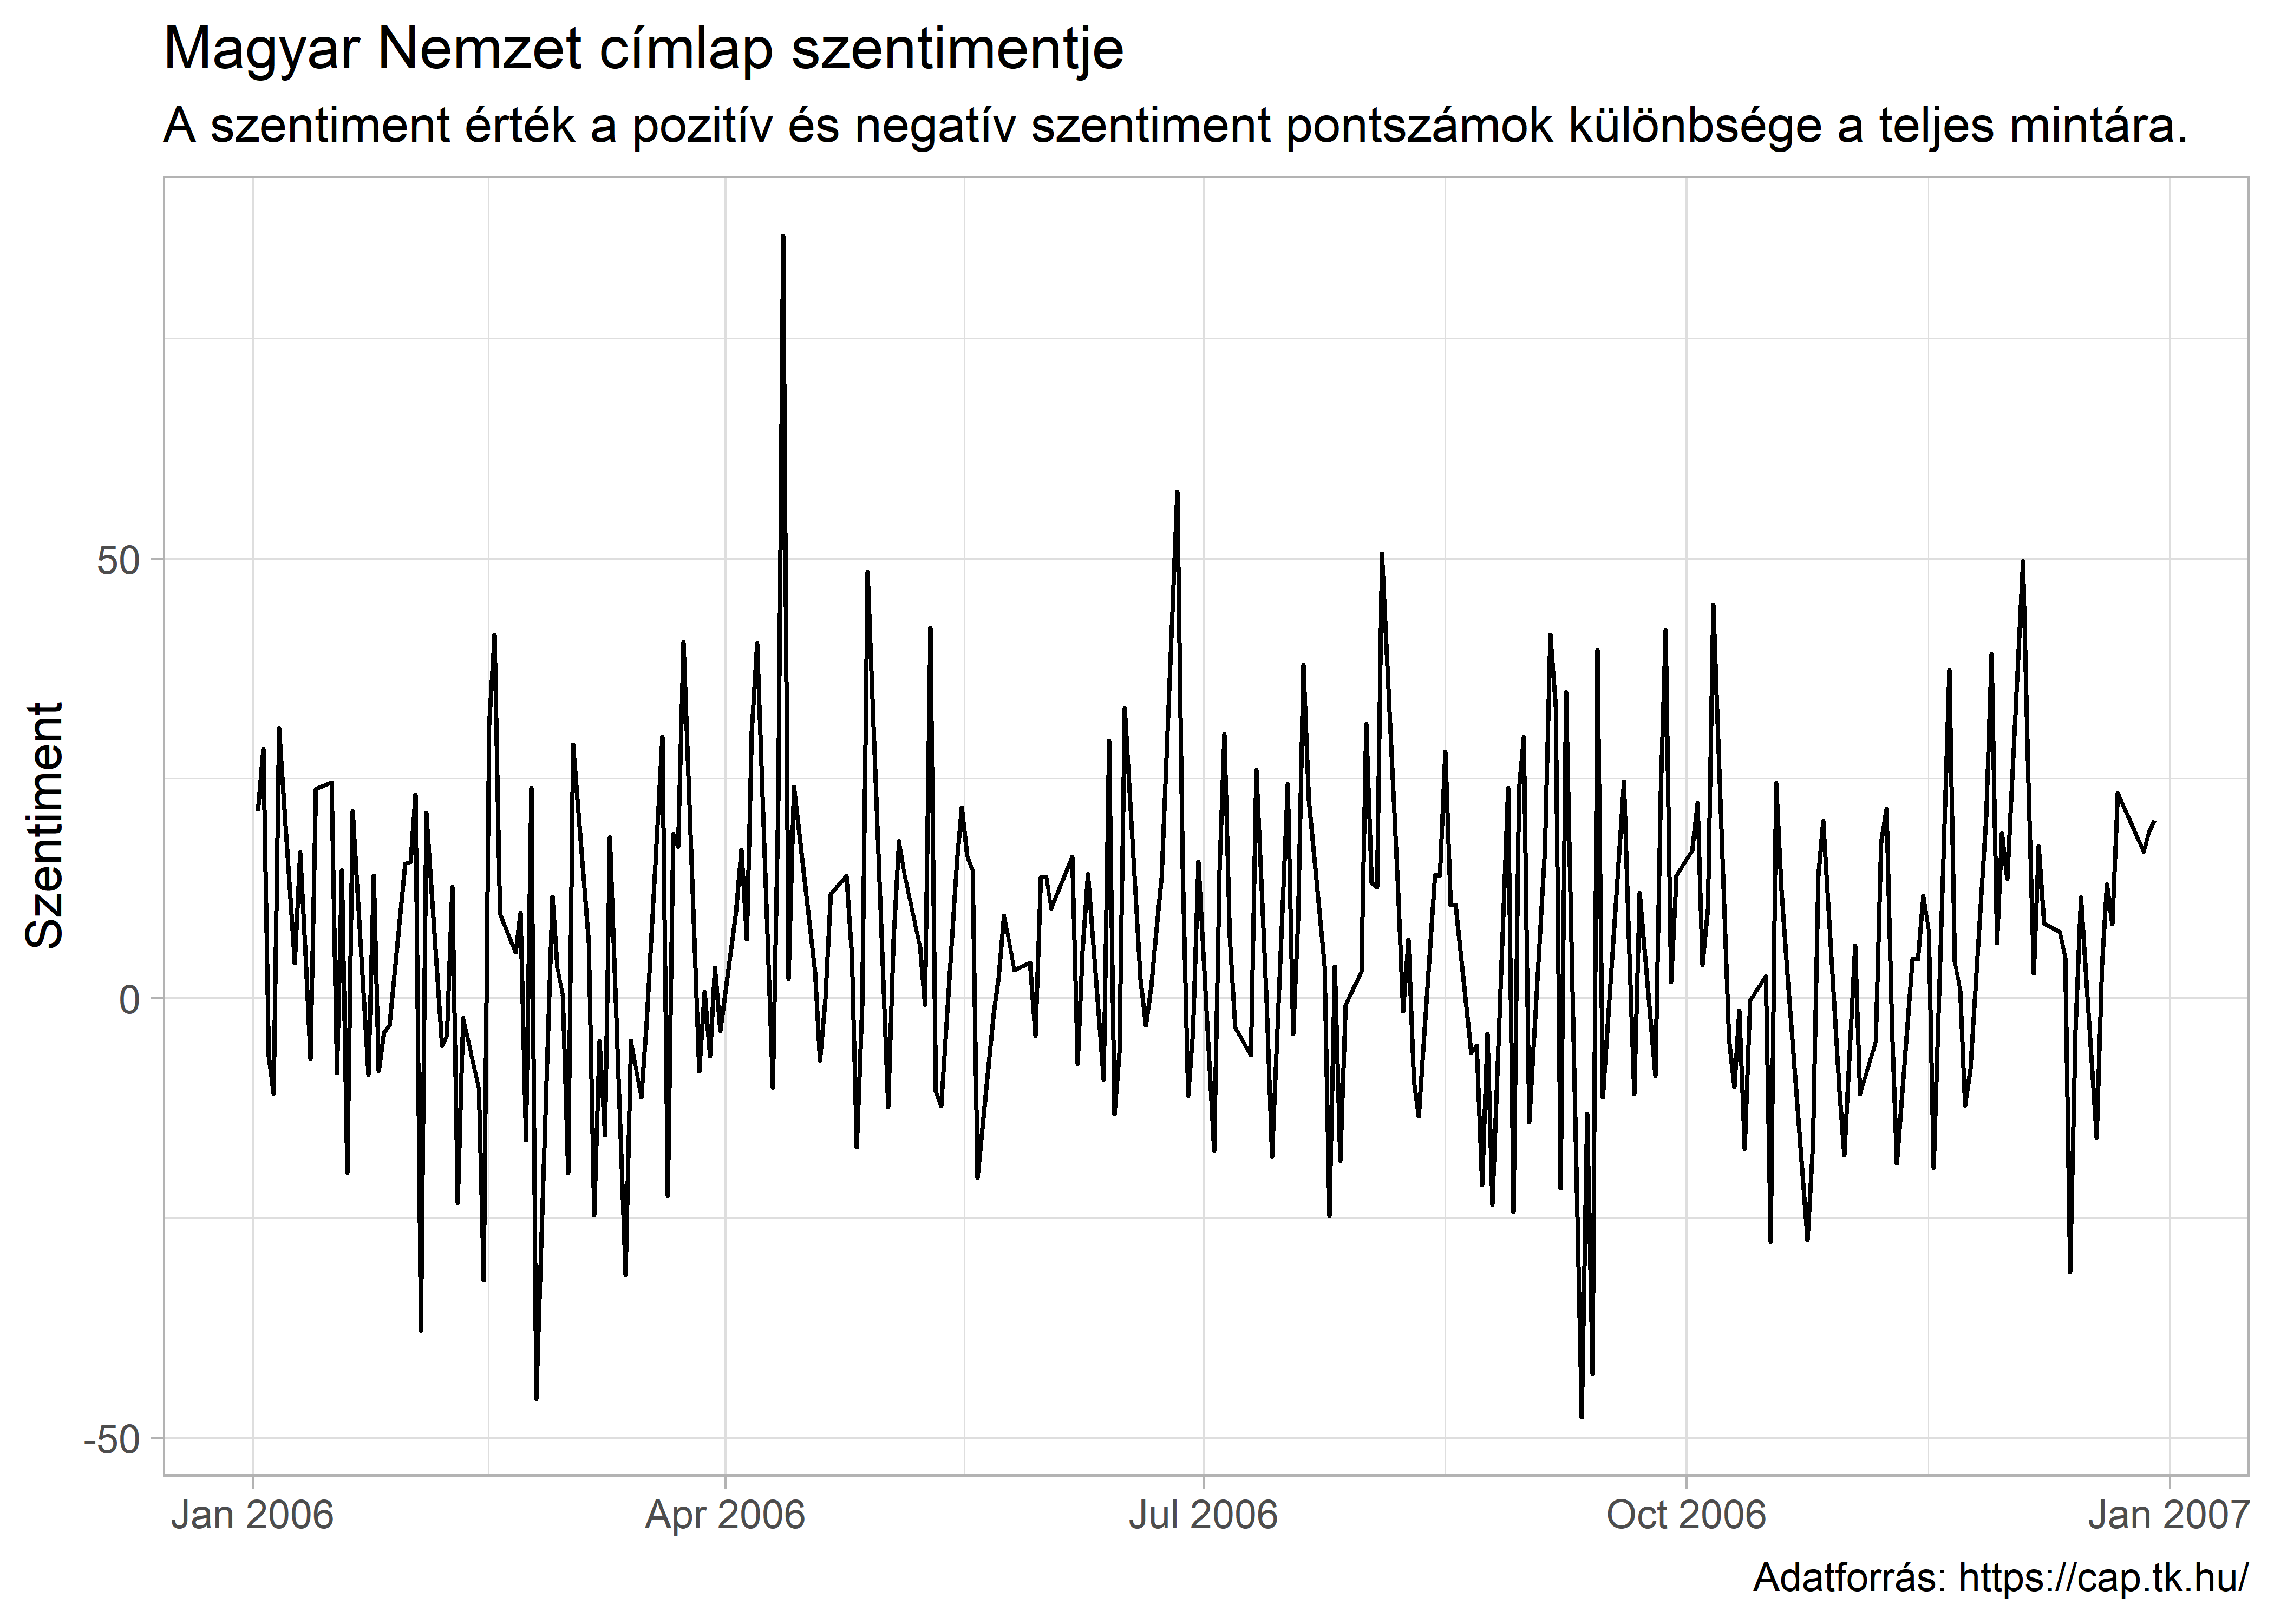
\includegraphics[width=0.9\linewidth]{_main_files/figure-latex/unnamed-chunk-55-1} \end{center}

\hypertarget{mnb-sajtuxf3kuxf6zlemuxe9nyek}{%
\section{MNB sajtóközlemények}\label{mnb-sajtuxf3kuxf6zlemuxe9nyek}}

A második esettanulmányban a kotextuális szótár elemzést mutatjuk be egy
angol nyelvű korpusz és specializált szótár segítségével. A korpusz az
MNB kamatdöntéseit kísérő nemzetközi sajtóközleményei és a szótár pedig
a \protect\hyperlink{ref-loughran2011}{Loughran and McDonald}
(\protect\hyperlink{ref-loughran2011}{2011}) pénzügyi
szentimentszótár.\footnote{A témával részletesebben is foglalkoztunk a
  \protect\hyperlink{ref-muxe1tuxe92021}{Máté, Sebők, and Barczikay}
  (\protect\hyperlink{ref-muxe1tuxe92021}{2021}) tanulmányban, ahol egy
  saját monetáris szentiment szótárt mutatunk be. Az implementáció és a
  hozzá tartozó R forráskód a nyilvános
  \url{https://doi.org/10.6084/m9.figshare.13526156.v1} linken.} A
szótár a \texttt{quanteda.dictionaries} csomag részeként elérhető,
illetve a tankönyv honlapján is megtalálható.

\begin{Shaded}
\begin{Highlighting}[]
\NormalTok{penzugy\_szentiment}
\CommentTok{\#\textgreater{} Dictionary object with 9 key entries.}
\CommentTok{\#\textgreater{} {-} [NEGATIVE]:}
\CommentTok{\#\textgreater{}   {-} abandon, abandoned, abandoning, abandonment, abandonments, abandons, abdicated, abdicates, abdicating, abdication, abdications, aberrant, aberration, aberrational, aberrations, abetting, abnormal, abnormalities, abnormality, abnormally [ ... and 2,335 more ]}
\CommentTok{\#\textgreater{} {-} [POSITIVE]:}
\CommentTok{\#\textgreater{}   {-} able, abundance, abundant, acclaimed, accomplish, accomplished, accomplishes, accomplishing, accomplishment, accomplishments, achieve, achieved, achievement, achievements, achieves, achieving, adequately, advancement, advancements, advances [ ... and 334 more ]}
\CommentTok{\#\textgreater{} {-} [UNCERTAINTY]:}
\CommentTok{\#\textgreater{}   {-} abeyance, abeyances, almost, alteration, alterations, ambiguities, ambiguity, ambiguous, anomalies, anomalous, anomalously, anomaly, anticipate, anticipated, anticipates, anticipating, anticipation, anticipations, apparent, apparently [ ... and 277 more ]}
\CommentTok{\#\textgreater{} {-} [LITIGIOUS]:}
\CommentTok{\#\textgreater{}   {-} abovementioned, abrogate, abrogated, abrogates, abrogating, abrogation, abrogations, absolve, absolved, absolves, absolving, accession, accessions, acquirees, acquirors, acquit, acquits, acquittal, acquittals, acquittance [ ... and 883 more ]}
\CommentTok{\#\textgreater{} {-} [CONSTRAINING]:}
\CommentTok{\#\textgreater{}   {-} abide, abiding, bound, bounded, commit, commitment, commitments, commits, committed, committing, compel, compelled, compelling, compels, comply, compulsion, compulsory, confine, confined, confinement [ ... and 164 more ]}
\CommentTok{\#\textgreater{} {-} [SUPERFLUOUS]:}
\CommentTok{\#\textgreater{}   {-} aegis, amorphous, anticipatory, appertaining, assimilate, assimilating, assimilation, bifurcated, bifurcation, cessions, cognizable, concomitant, correlative, deconsolidation, delineation, demonstrable, demonstrably, derecognized, derecognizes, derivatively [ ... and 36 more ]}
\CommentTok{\#\textgreater{} [ reached max\_nkey ... 3 more keys ]}
\end{Highlighting}
\end{Shaded}

A szentiment szótár 9 kategóriából áll. A legtöbb kulcsszó a negatív
dimenzióhoz van (2355).

A munkamenet hasonló a Magyar Nemzetes példához:

\begin{enumerate}
\def\labelenumi{\arabic{enumi}.}
\tightlist
\item
  adat betöltés
\item
  szövegtisztítás
\item
  korpusz
\item
  tokenek
\item
  kulcs kontextuális tokenek szűrése
\item
  dfm előállítás és szentiment számítás
\item
  az eredmény vizualizálása, további felhasználása
\end{enumerate}

\begin{Shaded}
\begin{Highlighting}[]
\NormalTok{mnb\_pr }\OtherTok{\textless{}{-}} \FunctionTok{read\_csv}\NormalTok{(}\StringTok{"data/mnb\_pr\_corpus.csv"}\NormalTok{)}

\FunctionTok{summary}\NormalTok{(mnb\_pr)}
\CommentTok{\#\textgreater{}       date                text                 id              year     }
\CommentTok{\#\textgreater{}  Min.   :2005{-}01{-}24   Length:180         Min.   :  1.00   Min.   :2005  }
\CommentTok{\#\textgreater{}  1st Qu.:2008{-}10{-}14   Class :character   1st Qu.: 45.75   1st Qu.:2008  }
\CommentTok{\#\textgreater{}  Median :2012{-}07{-}10   Mode  :character   Median : 90.50   Median :2012  }
\CommentTok{\#\textgreater{}  Mean   :2012{-}07{-}08                      Mean   : 90.50   Mean   :2012  }
\CommentTok{\#\textgreater{}  3rd Qu.:2016{-}03{-}30                      3rd Qu.:135.25   3rd Qu.:2016  }
\CommentTok{\#\textgreater{}  Max.   :2019{-}12{-}17                      Max.   :180.00   Max.   :2019}
\end{Highlighting}
\end{Shaded}

Az adatbázisunk 180 megfigyelésből és 4 változóbol áll. Az egyetlen
lényeges dokumentum meta adat itt is a szövegek megjelenési ideje.

A szövegeket ugyanazokkal a standard eszközökkel kezeljük mint a Magyar
Nemzet esetében. Érdemes minden esetben ellenőrízni, hogy az R kód amit
használunk az tényleg azt csinálja-e mint amit szeretnénk hogy
csináljon. Ez hatványozottan igaz abban az esetben, amikor szövegekkel
és regular expressionökkel dolgozunk.

\begin{Shaded}
\begin{Highlighting}[]
\NormalTok{mnb\_tiszta }\OtherTok{\textless{}{-}}\NormalTok{ mnb\_pr }\SpecialCharTok{\%\textgreater{}\%}
  \FunctionTok{mutate}\NormalTok{(}
    \AttributeTok{text =} \FunctionTok{str\_remove\_all}\NormalTok{(}\AttributeTok{string =}\NormalTok{ text, }\AttributeTok{pattern =} \StringTok{"[:cntrl:]"}\NormalTok{),}
    \AttributeTok{text =} \FunctionTok{str\_remove\_all}\NormalTok{(}\AttributeTok{string =}\NormalTok{ text, }\AttributeTok{pattern =} \StringTok{"[:punct:]"}\NormalTok{),}
    \AttributeTok{text =} \FunctionTok{str\_remove\_all}\NormalTok{(}\AttributeTok{string =}\NormalTok{ text, }\AttributeTok{pattern =} \StringTok{"[:digit:]"}\NormalTok{),}
    \AttributeTok{text =} \FunctionTok{str\_to\_lower}\NormalTok{(text),}
    \AttributeTok{text =} \FunctionTok{str\_trim}\NormalTok{(text),}
    \AttributeTok{text =} \FunctionTok{str\_squish}\NormalTok{(text)}
\NormalTok{  )}
\end{Highlighting}
\end{Shaded}

Miután rendelkezésre állnak a tiszta dokumentumaink, egy
karaktervektorba gyüjtjuk azokat a kulcsszavakat amelyek környékén
szeretnénk megfigyelni a szentiment alakulását. A példa kedvéért mi az
\texttt{unemp*}, \texttt{growth}, \texttt{gdp}, \texttt{inflation*}
szótöveket és szavakat választottuk. A \texttt{tokens\_keep()} megtartja
a kulcsszavainkat és egy általunk megadott +/- n tokenes környezetüket
(jelen esetben 10). A szentiment elemzést pedig már ezen a jóval kisebb
mátrixon fogjuk lefuttatni. A \texttt{phrase()} segítségével több szóból
álló kifejezéséket is vizsgálhatunk. Ilyen szókapcsolat például az
\emph{Európai Unió} is, ahol lényeges hogy egyben kezeljük a két szót.

\begin{Shaded}
\begin{Highlighting}[]
\NormalTok{mnb\_corpus }\OtherTok{\textless{}{-}} \FunctionTok{corpus}\NormalTok{(mnb\_tiszta)}

\NormalTok{gazdasag }\OtherTok{\textless{}{-}} \FunctionTok{c}\NormalTok{(}\StringTok{"unemp*"}\NormalTok{, }\StringTok{"growth"}\NormalTok{, }\StringTok{"gdp"}\NormalTok{, }\StringTok{"inflation*"}\NormalTok{, }\StringTok{"inflation expectation*"}\NormalTok{)}

\NormalTok{mnb\_token }\OtherTok{\textless{}{-}} \FunctionTok{tokens}\NormalTok{(mnb\_corpus) }\SpecialCharTok{\%\textgreater{}\%}
  \FunctionTok{tokens\_keep}\NormalTok{(}\AttributeTok{pattern =} \FunctionTok{phrase}\NormalTok{(gazdasag), }\AttributeTok{window =} \DecValTok{10}\NormalTok{)}
\end{Highlighting}
\end{Shaded}

A szentimentet most is egy súlyozott dfm-ből számoljuk. A kész eredményt
hozzáadjuk a korpuszhoz majd data framet hozunk létre belőle. A 9
kategóriából 5-öt adunk választunk csak ki, amelyeknek jegybanki
környezetben értelmezhető tartalma van.

\begin{Shaded}
\begin{Highlighting}[]
\NormalTok{mnb\_szentiment }\OtherTok{\textless{}{-}} \FunctionTok{tokens\_lookup}\NormalTok{(mnb\_token, }\AttributeTok{dictionary =}\NormalTok{ penzugy\_szentiment) }\SpecialCharTok{\%\textgreater{}\%}
  \FunctionTok{dfm}\NormalTok{() }\SpecialCharTok{\%\textgreater{}\%}
  \FunctionTok{dfm\_tfidf}\NormalTok{()}



\FunctionTok{docvars}\NormalTok{(mnb\_corpus, }\StringTok{"negative"}\NormalTok{) }\OtherTok{\textless{}{-}} \FunctionTok{as.numeric}\NormalTok{(mnb\_szentiment[, }\StringTok{"negative"}\NormalTok{])}
\FunctionTok{docvars}\NormalTok{(mnb\_corpus, }\StringTok{"positive"}\NormalTok{) }\OtherTok{\textless{}{-}} \FunctionTok{as.numeric}\NormalTok{(mnb\_szentiment[, }\StringTok{"positive"}\NormalTok{])}
\FunctionTok{docvars}\NormalTok{(mnb\_corpus, }\StringTok{"uncertainty"}\NormalTok{) }\OtherTok{\textless{}{-}} \FunctionTok{as.numeric}\NormalTok{(mnb\_szentiment[, }\StringTok{"uncertainty"}\NormalTok{])}
\FunctionTok{docvars}\NormalTok{(mnb\_corpus, }\StringTok{"constraining"}\NormalTok{) }\OtherTok{\textless{}{-}} \FunctionTok{as.numeric}\NormalTok{(mnb\_szentiment[, }\StringTok{"constraining"}\NormalTok{])}
\FunctionTok{docvars}\NormalTok{(mnb\_corpus, }\StringTok{"superfluous"}\NormalTok{) }\OtherTok{\textless{}{-}} \FunctionTok{as.numeric}\NormalTok{(mnb\_szentiment[, }\StringTok{"superfluous"}\NormalTok{])}


\NormalTok{mnb\_df }\OtherTok{\textless{}{-}} \FunctionTok{convert}\NormalTok{(mnb\_corpus, }\AttributeTok{to =} \StringTok{"data.frame"}\NormalTok{)}
\end{Highlighting}
\end{Shaded}

A célunk hogy szentiment kategóriánkénti bontásban mutassuk be az
elemzésünk eredményét, de előtte egy kicsit alakítani kell a data
frame-n, hogy a második fejezetben is tárgyalt \emph{tidy} formára
hozzuk. A különböző szentiment értékeket tartalmazó oszlopokat fogjuk
átrendezni úgy hogy kreálunk egy ``sent\_type'' változót ahol a
kategória nevet fogjuk eltárolni és egy ``sent\_score'' változót, ahol a
szentiment értéket. Ehhez a \texttt{tidyr}-ben található
\texttt{pivot\_longer()} -t használjuk.

\begin{Shaded}
\begin{Highlighting}[]
\NormalTok{mnb\_df }\OtherTok{\textless{}{-}}\NormalTok{ mnb\_df }\SpecialCharTok{\%\textgreater{}\%}
  \FunctionTok{pivot\_longer}\NormalTok{(}
    \AttributeTok{cols =}\NormalTok{ negative}\SpecialCharTok{:}\NormalTok{superfluous,}
    \AttributeTok{names\_to =} \StringTok{"sent\_type"}\NormalTok{,}
    \AttributeTok{values\_to =} \StringTok{"sent\_score"}
\NormalTok{  )}
\end{Highlighting}
\end{Shaded}

Az átalakítás után már könnyedén tudjuk kategóriákra bontva
megjeleníteni az MNB közlemények különböző látens dimenzióit. Fontos
emlékezni arra, hogy ez az eredmény a kulcsszavaink +/- 10 tokenes
környezetében lévő szavak szentimentjét mérik. Ami érdekes eredmény,
hogy a felesleges ``töltelék'' szövegek (superflous kategória) szinte
soha nem fordulnak elő a kulcsszavaink körül. A többi érték is nagyjából
megfelel a várakozásainknak, habár a 2008-as gazdasági válság nem tűnik
kiugró pontnak. Azonban a 2010 utáni európai válság már láthatóan
megjelnik az idősorainkban.

A szótár amit használtunk az alapvetően az Egyesült Államokban a tőzsdén
kereskedett cégek publikus beszámolóiból készült így elképzelhető, hogy
egyes jegybanki környezetben sokat használt kifejezés nincs benne. A
validálása a kapott eredményeknek ezért is nagyon fontos, illetve
érdemes azzal is tisztában lenni hogy a szótáras módszer nem tökéletes
(ahogy az emberi vagy más gépi kódolás sem).

\begin{Shaded}
\begin{Highlighting}[]
\FunctionTok{ggplot}\NormalTok{(mnb\_df, }\FunctionTok{aes}\NormalTok{(date, sent\_score)) }\SpecialCharTok{+}
  \FunctionTok{geom\_line}\NormalTok{() }\SpecialCharTok{+}
  \FunctionTok{labs}\NormalTok{(}
    \AttributeTok{title =} \StringTok{"Magyar Nemzeti Bank közleményeinek szentimentje"}\NormalTok{,}
    \AttributeTok{y =} \StringTok{"Szentiment"}\NormalTok{,}
    \AttributeTok{x =} \ConstantTok{NULL}
\NormalTok{  ) }\SpecialCharTok{+}
  \FunctionTok{facet\_wrap}\NormalTok{(}\SpecialCharTok{\textasciitilde{}}\NormalTok{sent\_type, }\AttributeTok{ncol =} \DecValTok{2}\NormalTok{)}
\end{Highlighting}
\end{Shaded}

\begin{center}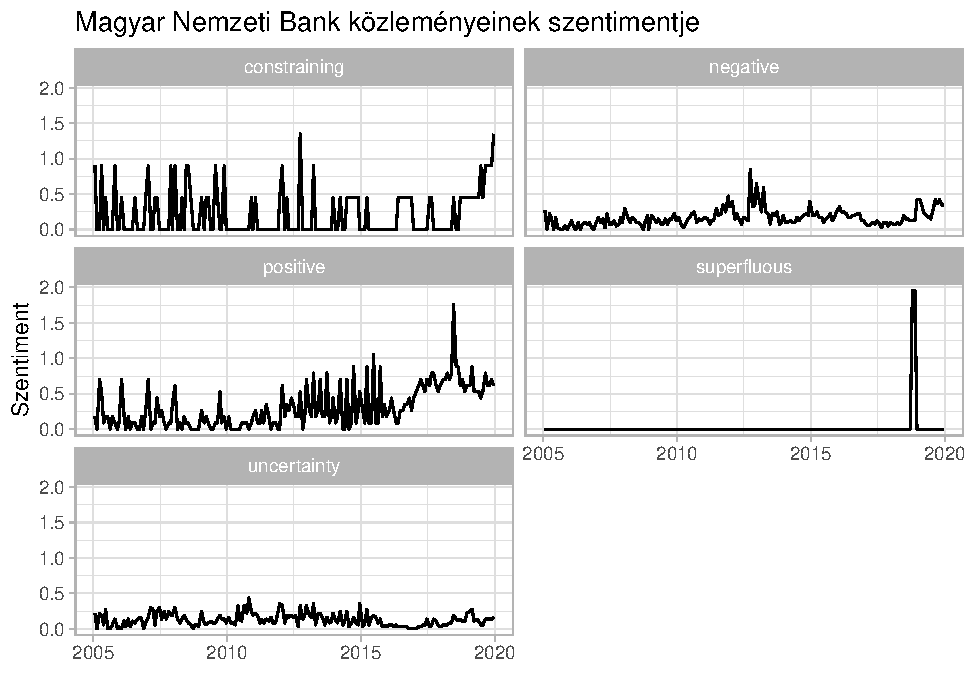
\includegraphics[width=0.9\linewidth]{_main_files/figure-latex/unnamed-chunk-63-1} \end{center}

\hypertarget{feluxfcgyelet-nuxe9lkuxfcli-tanuluxe1s-topik-modellezuxe9s-magyar-tuxf6rvuxe9nyszuxf6vegeken}{%
\chapter{Felügyelet nélküli tanulás: Topik modellezés magyar
törvényszövegeken}\label{feluxfcgyelet-nuxe9lkuxfcli-tanuluxe1s-topik-modellezuxe9s-magyar-tuxf6rvuxe9nyszuxf6vegeken}}

A klaszterezés egy adathalmaz pontjainak, rekordjainak hasonlóság
alapján való csoportosítása, ami szinte minden nagyméretű adathalmaz
leíró modellezésére alkalmas. A klaszterezés során az adatpontokat
diszjunkt halmazokba, azaz klaszterekbe soroljuk, hogy az elemeknek egy
olyan partíciója jöjjön létre, amelyben a közös csoportokba kerülő
elempárok lényegesen hasonlóbbak egymáshoz, mint azok a pontpárok,
melyek két különböző csoportba sorolódtak. Klaszterezés során a
megfelelő csoportok kialakítása nem egyértelmű feladat, mivel a
különböző adatok eltérő jelentése és felhasználása miatt
adathalmazonként más szempontokat kell figyelembe vennünk. Egy
klaszterezési feladat megoldásához ismernünk kell a különböző
algoritmusok alapvető tulajdonságait és mindig szükség van az
eredményként kapott klaszterezés kiértékelésére. Mivel egy klaszterezés
az adatpontok hasonlóságából indul ki, ezért az eljárás során az első
fontos lépés az adatpontok páronkénti hasonlóságát lehető legjobban
megragadó hasonlósági függvény kiválasztása
(\protect\hyperlink{ref-tan2011}{\textbf{tan2011?}}). Számos
klaszterezési eljárás létezik, melyek között az egyik leggyakoribb
különbségtétel, hogy a klaszterek egymásba ágyazottak vagy sem. Ez
alapján beszélhetünk hierarchikus és felosztó klaszterezésről.

A hierarchikus klaszterezés egymásba ágyazott klaszterek egy fába
rendezett halmaza, azaz ahol a klaszterek alklaszterekkel rendelkeznek.
A fa minden csúcsa (klasztere), a levélcsúcsokat kivéve, a gyermekei
(alklaszterei) uniója, és a fa gyökere az összes objektumot tartalmazó
klaszter. Felosztó (partitional) klaszterezés esetén az adathalmazt
olyan, nem átfedő alcsoportokra bontjuk, ahol minden adatobjektum
pontosan egy részhalmazba kerül
(\protect\hyperlink{ref-tikk2007}{\textbf{tikk2007?}};
\protect\hyperlink{ref-tan2011b}{\textbf{tan2011b?}}). A klaszterezési
eljárások között aszerint is különbséget tehetünk, hogy azok egy
objektumot csak egy vagy több klaszterbe is beilleszthetnek. Ez alapján
beszélhetünk kizáró (exclusive), illetve nem-kizáró (non exclusive),
vagy átfedő (overlapping) klaszterezésről. Az előbbi minden objektumot
csak egyetlen klaszterhez rendel hozzá, az utóbbi esetén egy pont több
klaszterbe is beleillik. Fuzzy klaszterezés esetén minden objektum
minden klaszterbe beletartozik egy tagsági súly erejéig, melynek értéke
0 (egyáltalán nem tartozik bele) és 1 (teljesen beletartozik) közé esik.
A klasztereknek is különböző típusai vannak, így beszélhetünk
prototípus-alapú, gráf-alapú vagy sűrűség-alapú klaszterekről.

A prototípus-alapú klaszter olyan objektumokat tartalmazó halmaz,
amelynek mindegyik objektuma jobban hasonlít a klasztert definiáló
objektumhoz, mint bármelyik másik klasztert definiáló objektumhoz. A
prototípus-alapú klaszter klaszterek közül a K-közép klaszter az egyik
leggyakrabban alkalmazott. A K-közép klaszterezési módszer első lépése K
darab kezdő középpontot kijelölése, ahol K a klaszterek kívánt számával
egyenlő. Ezután minden adatpontot a hozzá legközelebb eső középponthoz
rendelünk. Az így képzett csoportok lesznek a kiinduló klaszterek.
Ezután újra meghatározzuk mindegyik klaszter középpontját a klaszterhez
rendelt pontok alapján. A hozzárendelési és frissítési lépéseket
felváltva folytatjuk addig, amíg egyetlen pont sem vált klasztert, vagy
ameddig a középpontok ugyanazok nem maradnak
(\protect\hyperlink{ref-tan2011c}{\textbf{tan2011c?}}).

\hypertarget{k-kuxf6zuxe9p-klaszterezuxe9s-kvalitatuxedv-adatokkal}{%
\section{K közép klaszterezés kvalitatív
adatokkal}\label{k-kuxf6zuxe9p-klaszterezuxe9s-kvalitatuxedv-adatokkal}}

A K közép klaszterezés tehát a dokumentumokat alkotó szavak alapján
keresi meg a felhasználó által megadott számú (K) klasztert, amelyeket a
középpontjaik képviselnek, és így rendezi a dokumentumokat csoportokba.
A klaszterezés vagy csoportosítás egy induktív kategorizálás, ami akkor
hasznos, amikor nem állnak a kutató rendelkezésére előzetesen ismert
csoportok, amelyek szerint a vizsgált dokumentumokat rendezni tudná.
Hiszen ebben az esetben a korpusz elemeinek rendezéséhez nem határozunk
meg előzetesen csoportokat, hanem az eljárás során olyan különálló
csoportokat hozunk létre a dokumentumokból, amelynek tagjai valamilyen
szempontból hasonlítanak egymásra. A csoportosítás legfőbb célja az,
hogy az egy csoportba kerülő szövegek minél inkább hasonlítsanak
egymásra, miközben a különböző csoportba kerülők minél inkább eltérjenek
egymástól. Azaz klaszterezésnél nem egy-egy szöveg jellemzőire vagyunk
kíváncsiak, hanem arra, hogy a szövegek egy-egy csoportja milyen
hasonlóságokkal bír.
(\protect\hyperlink{ref-tikk2007a}{\textbf{tikk2007a?}} ;
\protect\hyperlink{ref-burtejin2016}{\textbf{burtejin2016?}}) A gépi
kódolással végzett klaszterezés egy felügyelet nélküli tanulás, mely a
szöveg tulajdonságaiból tanul, anélkül, hogy előre meghatározott
csoportokat ismerne. Alkalmazása során a dokumentum tulajdonságait és a
modell becsléseit felhasználva jönnek létre a különböző kategóriák,
melyekhez később hozzárendeli a szöveget
(\protect\hyperlink{ref-grimmer2013:15}{\textbf{grimmer2013:15?}}). Az
osztályozással ellentétben a csoportosítás esetén tehát nincs ismert
„címkékkel" ellátott kategóriarendszer vagy olyan minta, mint az
osztályozás esetében a tanítókörnyezet, amiből tanulva a modellt fel
lehet építeni
(\protect\hyperlink{ref-tikk2007b:145}{\textbf{tikk2007b:145?}}). A gépi
kódolással végzett csoportosítás (klaszterezés) esetén a kutató feladata
a megfelelő csoportosító mechanizmus kiválasztása, mely alapján egy
program végzi el a szövegek különböző kategóriákba sorolását. Ezt követi
a hasonló szövegeket tömörítő csoportok elnevezésének lépése. A több
dokumentumból álló korpuszok esetében a gépi klaszterelemzés különösen
eredményes és költséghatékony lehet, mivel egy nagy korpusz vizsgálata
sok erőforrást igényel
(\protect\hyperlink{ref-grimmer2013a:1}{\textbf{grimmer2013a:1?}}).

A klaszterezés bemutatásához a rendszerváltás utáni magyar
miniszterelnökök egy-egy véletlenszerűen kiválasztott beszédét
használjuk.

\begin{Shaded}
\begin{Highlighting}[]

\FunctionTok{library}\NormalTok{(readr)}
\FunctionTok{library}\NormalTok{(dplyr)}
\FunctionTok{library}\NormalTok{(stringr)}
\FunctionTok{library}\NormalTok{(readtext)}
\FunctionTok{library}\NormalTok{(quanteda)}
\FunctionTok{library}\NormalTok{(ggplot2)}
\FunctionTok{library}\NormalTok{(topicmodels)}
\FunctionTok{library}\NormalTok{(factoextra)}
\end{Highlighting}
\end{Shaded}

A beszédek szövege meglehetősen tiszta, ezért az egyszerűség kedvéért a
most kihagyjuk a szövegtisztítás lépéseit. Az elemzés első lépéseként a
\texttt{quanteda} csomaggal egy korpusz kreálunk, majd abból egy
dokumentum-kifejezés mátrixot készítünk a \texttt{dfm()} függvénnyel.

\begin{Shaded}
\begin{Highlighting}[]
\NormalTok{beszedek }\OtherTok{\textless{}{-}} \FunctionTok{read\_csv}\NormalTok{(}\StringTok{"data/miniszterelnokok.csv"}\NormalTok{)}

\NormalTok{beszedek\_corpus }\OtherTok{\textless{}{-}} \FunctionTok{corpus}\NormalTok{(beszedek)}

\NormalTok{beszedek\_dfm }\OtherTok{\textless{}{-}} \FunctionTok{dfm}\NormalTok{(beszedek\_corpus)}
\end{Highlighting}
\end{Shaded}

A beszédek klaszterekbe rendezését az R egyik alapfüggvénye végzi, a
\texttt{kmeans}. Első lépésben 3 klasztert készítünk. A \texttt{table()}
függvénnyel megnézhetjük hogy egy-egy csoportba hány dokumentum került.

\begin{Shaded}
\begin{Highlighting}[]
\NormalTok{beszedek\_klaszter }\OtherTok{\textless{}{-}} \FunctionTok{kmeans}\NormalTok{(beszedek\_dfm, }\AttributeTok{centers =} \DecValTok{2}\NormalTok{)}


\FunctionTok{table}\NormalTok{(beszedek\_klaszter}\SpecialCharTok{$}\NormalTok{cluster)}
\CommentTok{\#\textgreater{} }
\CommentTok{\#\textgreater{} 1 2 }
\CommentTok{\#\textgreater{} 2 5}
\end{Highlighting}
\end{Shaded}

A felügyelet nélküli klasszifikáció nagy kérdése, hogy hány klasztert
készítsünk, hogy megközelítsük a valóságot és ne csak mesterségesen
kreáljunk csoportokat abban az esetben is amikor ténylegesen nem
léteznek. A kvalitatív megközelítések mellett kvantitatív opciók is
vannak. A \texttt{factoextra} csomagban több ilyen módszer is van
implementálva. A lenti ábra azt mutatja hogy a klasztereken belüli
négyzetösszegek hogyan változnak a \emph{k} paraméter változásának
függvényében. A lenti ábra alapján az ideális klaszter szám 2.

\begin{Shaded}
\begin{Highlighting}[]

\FunctionTok{fviz\_nbclust}\NormalTok{(}\FunctionTok{as.matrix}\NormalTok{(beszedek\_dfm), kmeans, }\AttributeTok{method =} \StringTok{"wss"}\NormalTok{, }\AttributeTok{k.max =} \DecValTok{5}\NormalTok{)}
\end{Highlighting}
\end{Shaded}

\begin{center}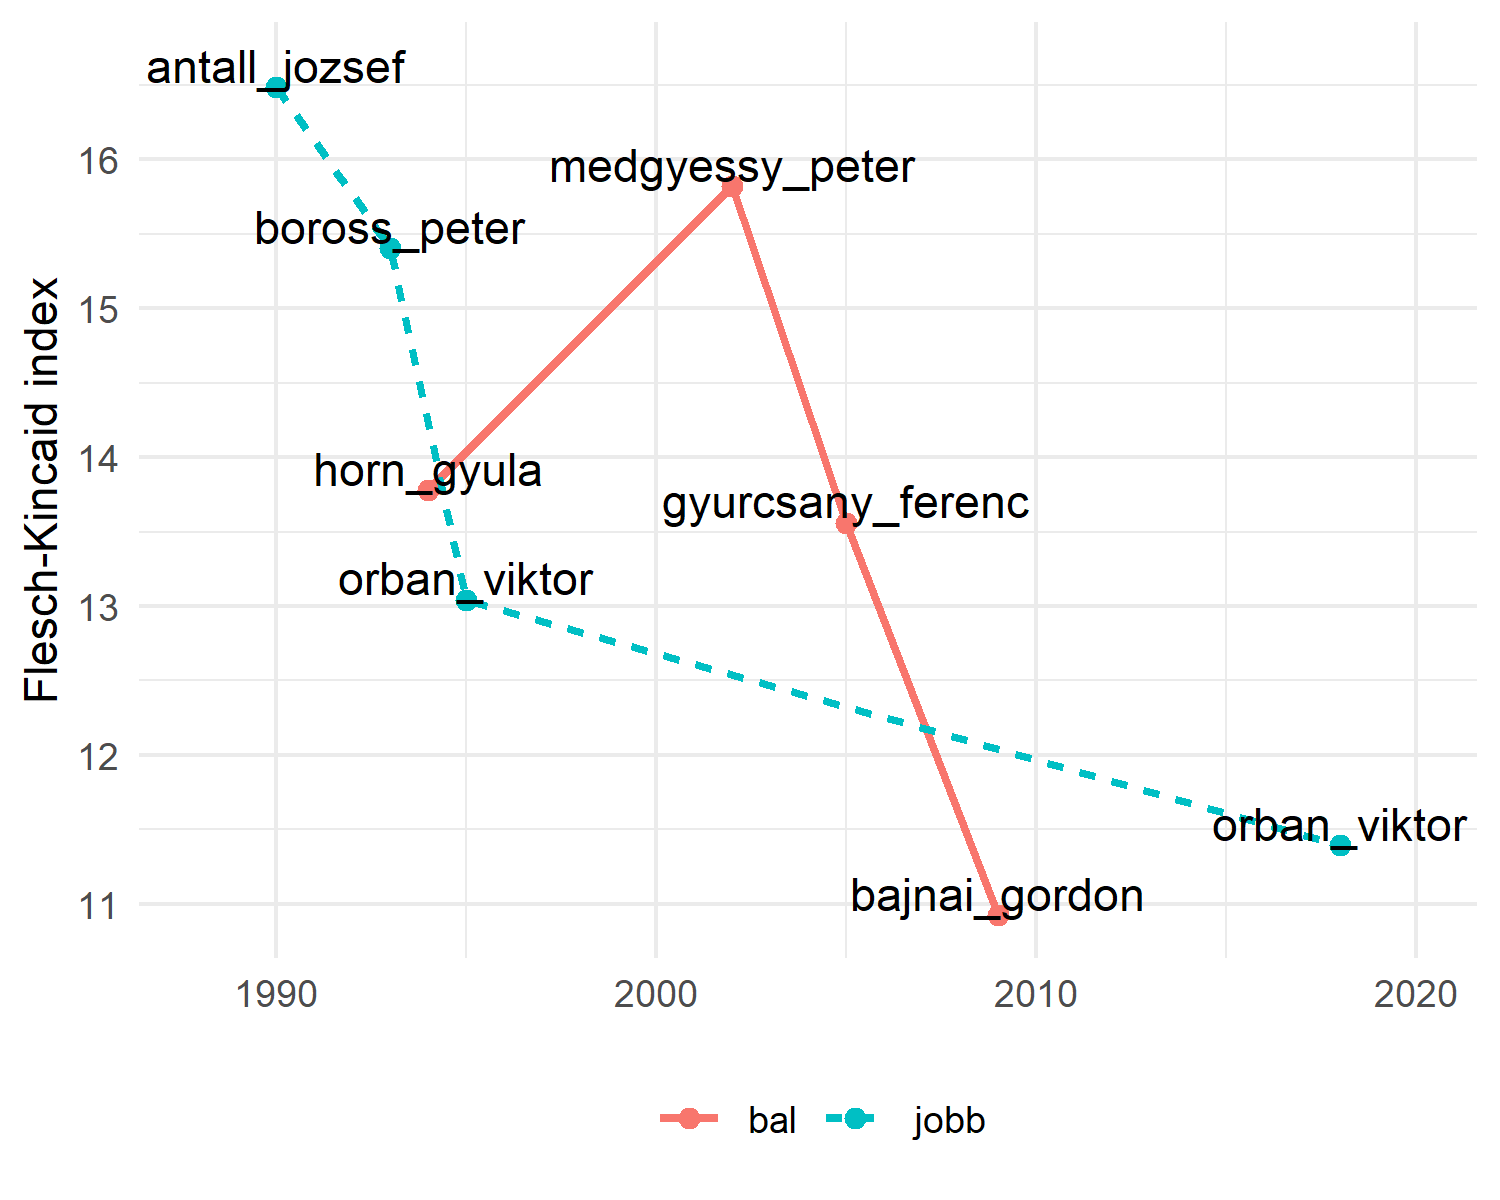
\includegraphics[width=0.9\linewidth]{_main_files/figure-latex/unnamed-chunk-67-1} \end{center}

Vizuálisan is megjeleníthetjük a kialakított csoportokat.

\begin{Shaded}
\begin{Highlighting}[]
\FunctionTok{fviz\_cluster}\NormalTok{(beszedek\_klaszter, }\AttributeTok{data =}\NormalTok{ beszedek\_dfm)}
\end{Highlighting}
\end{Shaded}

\begin{center}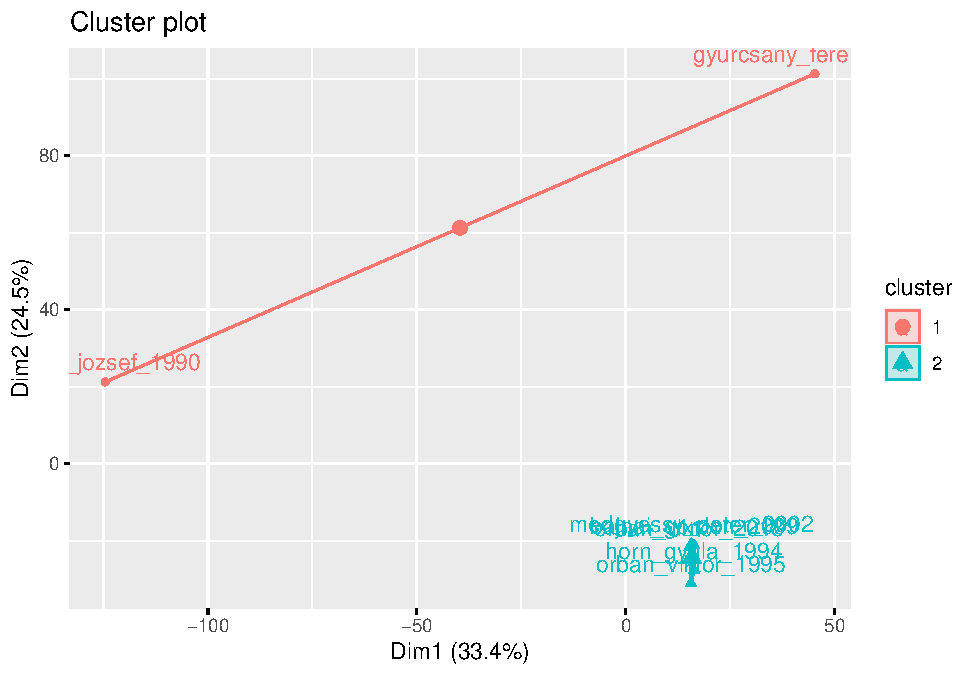
\includegraphics[width=0.9\linewidth]{_main_files/figure-latex/unnamed-chunk-68-1} \end{center}

\hypertarget{luxe1tens-dirichlet-allokuxe1ciuxf3-topik-modellekklasztering_topicmodellek-2}{%
\section[Látens Dirichlet Allokáció topik
modellek]{\texorpdfstring{Látens Dirichlet Allokáció topik
modellek\footnote{a kód részben az alábbiakon alapul:
  tidytextmining.com/topicmodeling.html Az általunk is használt
  \texttt{topicmodels} csomag interfészt biztosít az LDA modellek és a
  korrelált témamodellek (CTM) C kódjához, valamint az LDA modellek
  illesztéséhez szükséges C ++ kódhoz.}}{Látens Dirichlet Allokáció topik modellek}}\label{luxe1tens-dirichlet-allokuxe1ciuxf3-topik-modellekklasztering_topicmodellek-2}}

A topik-modellezés a dokumentumok téma-klasztereinek meghatározására
szolgáló valószínűség-alapú eljárás, amely szó-gyakoriságot állapít meg
minden témához, és minden dokumentumhoz hozzárendeli az adott témák
valószínűségét. A topik modellezés egy felügyelet nélküli tanulási
módszer, amely során az alkalmazott algoritmus a dokumentum
tulajdonságait és a modell becsléseit felhasználva hoz létre különböző
kategóriákat, melyekhez később hozzárendeli a szöveget
(\protect\hyperlink{ref-tikk2007c}{\textbf{tikk2007c?}};
\protect\hyperlink{ref-grimmer2013b}{\textbf{grimmer2013b?}};
\protect\hyperlink{ref-burtejin2016a}{\textbf{burtejin2016a?}}). Az
egyik leggyakrabban alkalmazott topik modellezési eljárás, a Látens
Dirichlet Allokáció (LDA) alapja az a feltételezés, hogy minden korpusz
topikok/témák keverékéből áll, ezen témák pedig statisztikailag a
korpusz szókészlete valószínűségi függvényeinek (eloszlásának)
tekinthetőek (\protect\hyperlink{ref-blei2003}{\textbf{blei2003?}}). Az
LDA a korpusz dokumentumainak csoportosítása során az egyes
dokumentumokhoz topik szavakat rendel, a topikok megbecsléséhez pedig a
szavak együttes megjelenését vizsgálja a dokumentum egészében. Az LDA
algoritmusnak előzetesen meg kell adni a keresett klaszterek (azaz a
keresett topikok) számát, ezt követően a dokumentumhalmazban szereplő
szavak eloszlása alapján az algoritmus azonosítja a kulcsszavakat,
amelyek eloszlása kirajzolja a topikokat
(\protect\hyperlink{ref-blei2003a}{\textbf{blei2003a?}};
\protect\hyperlink{ref-burtejin2016b}{\textbf{burtejin2016b?}};
\protect\hyperlink{ref-jacobi2016}{Jacobi, Van Atteveldt, and Welbers
2016}).

\begin{center}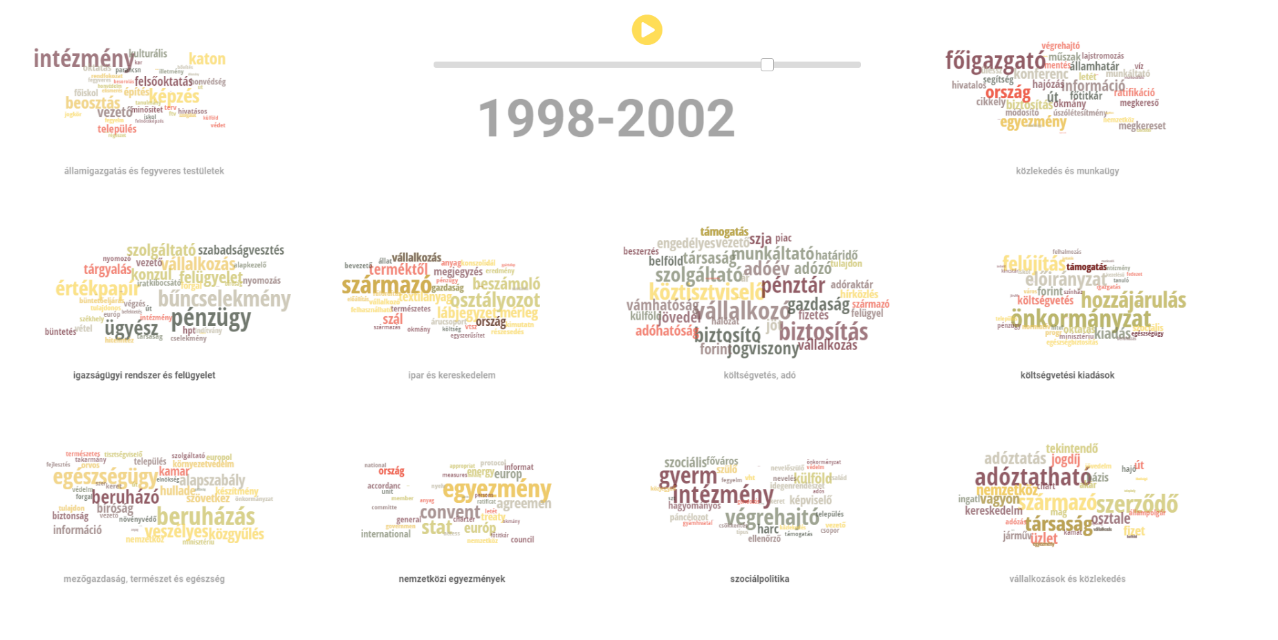
\includegraphics[width=0.9\linewidth]{figures/08-01_topik_modell} \end{center}

A következőkben a magyar törvények korpuszán szemléltetjük a topik
modellezés módszerét, hogy a mesterséges intelligencia segítségével
feltárjuk a korpuszon belüli rejtett összefüggéseket. A korábban leírtak
szerint tehát nincsenek előre meghatározott kategóriáink,
dokumentumainkat a klaszterezés segítségével szeretnénk csoportosítani.
Egy-egy dokumentumban keveredhetnek a témák és az azokat reprezentáló
szavak. Mivel ugyanaz a szó több topikhoz is kapcsolódhat, így az
eljárás komplex elemzési lehetőséget nyújt, az egy szövegen belül témák
és akár azok dokumentumon belüli súlyának azonosítására. Példánkban csak
a korpusz egy részén szemléltetjük a topik modellezést, a teljes korpusz
és annak elemzéséhez szükséges kód elérhető az alábbi github linken:
\url{https://github.com/poltextlab}

Az alábbiakban 1998-2002 és a 2002-2006-os parlamenti ciklus 1032
törvényszövegének topik modellezését és a szükséges előkészítő,
korpusztisztító lépéseket mutatjuk be. Az következőkben használt fájlok
letölthetőek az alábbi github linkről:
\url{https://github.com/poltextlab/text_mining_with_r} A fájlokat
töltsük be az R által használt munkakönyvtárba.\footnote{A teljes
  törvényeket és a metadatokat tartalmazó adatbázisokat a
  \url{https://cap.tk.hu/} honlapról lehet letölteni.}

Töltsük be az elemezni kívánt csv fájlt, megadva az elérési útvonalát.

\begin{Shaded}
\begin{Highlighting}[]
\NormalTok{torvenyek }\OtherTok{\textless{}{-}} \FunctionTok{read\_csv}\NormalTok{(}\StringTok{"data/lawtext\_1998\_2006.csv"}\NormalTok{)}
\end{Highlighting}
\end{Shaded}

Az előző fejezetekben láthattuk hogy hogyan lehet használni a
\texttt{stringr} csomagot a szövegtisztításra. A lépések a már megismert
sztenderd folyamatot követik: számok, központozás, sortörések, extra
szóközök eltávolítása, illetve a szöveg kisbetűsítése. Az eddigieket
további szövegtisztító lépésekkel is kiegészíthetjük. Olyan elemek
esetében, amelyek nem feltétlenül különálló szavak és el akarjuk
távolítani őket a korpuszból szintén az \texttt{str\_remove\_all()} a
legegyszerűbb megoldás.

\begin{Shaded}
\begin{Highlighting}[]
\NormalTok{torvenyek\_tiszta }\OtherTok{\textless{}{-}}\NormalTok{ torvenyek }\SpecialCharTok{\%\textgreater{}\%}
  \FunctionTok{mutate}\NormalTok{(}
    \AttributeTok{text =} \FunctionTok{str\_remove\_all}\NormalTok{(}\AttributeTok{string =}\NormalTok{ text, }\AttributeTok{pattern =} \StringTok{"[:cntrl:]"}\NormalTok{),}
    \AttributeTok{text =} \FunctionTok{str\_remove\_all}\NormalTok{(}\AttributeTok{string =}\NormalTok{ text, }\AttributeTok{pattern =} \StringTok{"[:punct:]"}\NormalTok{),}
    \AttributeTok{text =} \FunctionTok{str\_remove\_all}\NormalTok{(}\AttributeTok{string =}\NormalTok{ text, }\AttributeTok{pattern =} \StringTok{"[:digit:]"}\NormalTok{),}
    \AttributeTok{text =} \FunctionTok{str\_to\_lower}\NormalTok{(text),}
    \AttributeTok{text =} \FunctionTok{str\_trim}\NormalTok{(text),}
    \AttributeTok{text =} \FunctionTok{str\_squish}\NormalTok{(text),}
    \AttributeTok{text =} \FunctionTok{str\_remove\_all}\NormalTok{(}\AttributeTok{string =}\NormalTok{ text, }\AttributeTok{pattern =} \StringTok{"’"}\NormalTok{),}
    \AttributeTok{text =} \FunctionTok{str\_remove\_all}\NormalTok{(}\AttributeTok{string =}\NormalTok{ text, }\AttributeTok{pattern =} \StringTok{"…"}\NormalTok{),}
    \AttributeTok{text =} \FunctionTok{str\_remove\_all}\NormalTok{(}\AttributeTok{string =}\NormalTok{ text, }\AttributeTok{pattern =} \StringTok{"–"}\NormalTok{),}
    \AttributeTok{text =} \FunctionTok{str\_remove\_all}\NormalTok{(}\AttributeTok{string =}\NormalTok{ text, }\AttributeTok{pattern =} \StringTok{"“"}\NormalTok{),}
    \AttributeTok{text =} \FunctionTok{str\_remove\_all}\NormalTok{(}\AttributeTok{string =}\NormalTok{ text, }\AttributeTok{pattern =} \StringTok{"”"}\NormalTok{),}
    \AttributeTok{text =} \FunctionTok{str\_remove\_all}\NormalTok{(}\AttributeTok{string =}\NormalTok{ text, }\AttributeTok{pattern =} \StringTok{"„"}\NormalTok{),}
    \AttributeTok{text =} \FunctionTok{str\_remove\_all}\NormalTok{(}\AttributeTok{string =}\NormalTok{ text, }\AttributeTok{pattern =} \StringTok{"«"}\NormalTok{),}
    \AttributeTok{text =} \FunctionTok{str\_remove\_all}\NormalTok{(}\AttributeTok{string =}\NormalTok{ text, }\AttributeTok{pattern =} \StringTok{"»"}\NormalTok{),}
    \AttributeTok{text =} \FunctionTok{str\_remove\_all}\NormalTok{(}\AttributeTok{string =}\NormalTok{ text, }\AttributeTok{pattern =} \StringTok{"§"}\NormalTok{),}
    \AttributeTok{text =} \FunctionTok{str\_remove\_all}\NormalTok{(}\AttributeTok{string =}\NormalTok{ text, }\AttributeTok{pattern =} \StringTok{"°"}\NormalTok{),}
    \AttributeTok{text =} \FunctionTok{str\_remove\_all}\NormalTok{(}\AttributeTok{string =}\NormalTok{ text, }\AttributeTok{pattern =} \StringTok{"\textless{}U+25A1\textgreater{}"}\NormalTok{),}
    \AttributeTok{text =} \FunctionTok{str\_remove\_all}\NormalTok{(}\AttributeTok{string =}\NormalTok{ text, }\AttributeTok{pattern =} \StringTok{"\textless{}U+25A1\textgreater{}"}\NormalTok{),}
    \AttributeTok{text =} \FunctionTok{str\_remove\_all}\NormalTok{(}\AttributeTok{string =}\NormalTok{ text, }\AttributeTok{pattern =} \StringTok{"@"}\NormalTok{)}
\NormalTok{  )}
\end{Highlighting}
\end{Shaded}

A dokumentum változókat egy külön fájlból adjuk hozzá, ami a törvények
keletkezési évét tartalmazza, illetve hogy melyik kormányzati ciklusban
születtek. Mindkét adatbázisban egy közös egyedi azonosító jelöli az
egyes törvényeket, így ki tudjuk használni a \texttt{dplyr}
\texttt{left\_join()} függvényét, ami hatékonyan és gyorsan kapcsol
össze adatbázisokat közös egyedi azonosító mentén. Jelen esetben ez az
egyedi azonosító a \texttt{txt\_filename} oszlopból fog elkészülni,
amely a torvenyek neveit tartalmazza. Első lépésben betöltjük a meta
adatokat tartalmazó .csv fájlt, majd a \texttt{.txt} rész előtti
törvényneveket tartjuk csak meg a létrehozott \texttt{doc\_id}-
oszlopban. A \texttt{{[}\^{}\textbackslash{}\textbackslash{}.{]}*}
regular expression itt a string elejétől indulva kijelöl mindent az elso
\texttt{.} karakterig. Az \texttt{str\_extract()} pedig ezt a kijelölt
string szakaszt (ami a törvények neve) menti át az új változónkba.

\begin{Shaded}
\begin{Highlighting}[]
\NormalTok{torveny\_meta }\OtherTok{\textless{}{-}} \FunctionTok{read\_csv}\NormalTok{(}\StringTok{"data/cap\_law\_meta.csv"}\NormalTok{)}

\NormalTok{torveny\_meta }\OtherTok{\textless{}{-}}\NormalTok{ torveny\_meta }\SpecialCharTok{\%\textgreater{}\%}
  \FunctionTok{mutate}\NormalTok{(}\AttributeTok{doc\_id =} \FunctionTok{str\_extract}\NormalTok{(txt\_filename, }\StringTok{"[\^{}}\SpecialCharTok{\textbackslash{}\textbackslash{}}\StringTok{.]*"}\NormalTok{)) }\SpecialCharTok{\%\textgreater{}\%}
  \FunctionTok{select}\NormalTok{(}\SpecialCharTok{{-}}\NormalTok{txt\_filename)}

\FunctionTok{head}\NormalTok{(torveny\_meta, }\DecValTok{5}\NormalTok{)}
\CommentTok{\#\textgreater{} \# A tibble: 5 x 4}
\CommentTok{\#\textgreater{}    year electoral\_cycle majortopic doc\_id     }
\CommentTok{\#\textgreater{}   \textless{}dbl\textgreater{} \textless{}chr\textgreater{}                \textless{}dbl\textgreater{} \textless{}chr\textgreater{}      }
\CommentTok{\#\textgreater{} 1  1998 1998{-}2002               13 1998XXXV   }
\CommentTok{\#\textgreater{} 2  1998 1998{-}2002               20 1998XXXVI  }
\CommentTok{\#\textgreater{} 3  1998 1998{-}2002                3 1998XXXVII }
\CommentTok{\#\textgreater{} 4  1998 1998{-}2002                6 1998XXXVIII}
\CommentTok{\#\textgreater{} 5  1998 1998{-}2002               13 1998XXXIX}
\end{Highlighting}
\end{Shaded}

Végül összefűzzük a dokumentumokat és a meta adatokat tartalmazó data
frameket.

\begin{Shaded}
\begin{Highlighting}[]
\NormalTok{torveny\_final }\OtherTok{\textless{}{-}} \FunctionTok{left\_join}\NormalTok{(torvenyek\_tiszta, torveny\_meta, }\AttributeTok{by =} \StringTok{"doc\_id"}\NormalTok{)}
\end{Highlighting}
\end{Shaded}

Majd hozzuk létre a korpuszt és ellenőrizzük azt.

\begin{verbatim}
#>       Text Types Tokens Sentences year electoral_cycle majortopic
#> 1    1998L  2879   9628         1 1998       1998-2002          3
#> 2   1998LI   352    680         1 1998       1998-2002         20
#> 3  1998LII   446    992         1 1998       1998-2002          9
#> 4 1998LIII   126    221         1 1998       1998-2002          9
#> 5  1998LIV   835   2013         1 1998       1998-2002          9
\end{verbatim}

Az RStudio environments fülén láthatjuk, hogy egy 1032 elemből álló
korpusz jött létre, amelynek tartalmát a \texttt{summary()} paranccsal
kiíratva a console ablakban megjelenik a dokumentumok listája és a főbb
leíró statisztikai adatok (egyedi szavak - types; szószám - tokens;
mondatok - sentences). Az előbbi fejezettől eltérően most a tokenizálás
során is végzünk még egy kis tisztítást: a felesleges stop szavakat
kitöröljük a \texttt{tokens\_remove()} és \texttt{stopwords()}
kombinálásával. A \texttt{quanteda} tartalmaz egy beépített magyar
stopszó szótárat. A második lépésben szótövesítjük a tokeneket a
\texttt{tokens\_words()} használatával, ami szintén képes a magyar
nyelvű szövegeket kezelni.

Szükség esetén a beépített magyar nyelvű stopszó szótárat saját
stopszavakkal is kiegészíthetjük. Ehhez először \texttt{csv} fájlba el
kell mentenünk a stopszavakat, majd a \texttt{csv} fájlt be kell
olvasnunk. Az \texttt{pull()} egy karaktervektort fog kreálni a data
frame \texttt{text} oszlopából.

\begin{Shaded}
\begin{Highlighting}[]
\NormalTok{custom\_stopwords }\OtherTok{\textless{}{-}} \FunctionTok{readtext}\NormalTok{(}\StringTok{"data/custom\_legal\_stopwords.csv"}\NormalTok{, }\AttributeTok{encoding =} \StringTok{"UTF8"}\NormalTok{) }\SpecialCharTok{\%\textgreater{}\%}
  \FunctionTok{pull}\NormalTok{(text)}
\end{Highlighting}
\end{Shaded}

Mivel jogi szövegekről van szó, ezért még egy kis extra szószedetet is
készítűnk a felesleges szavakról.

\begin{Shaded}
\begin{Highlighting}[]
\NormalTok{custom\_stopwords\_egyeb }\OtherTok{\textless{}{-}} \FunctionTok{c}\NormalTok{(}\StringTok{"lábjegyzet"}\NormalTok{, }\StringTok{"országgyulés"}\NormalTok{, }\StringTok{"ülésnap"}\NormalTok{)}
\end{Highlighting}
\end{Shaded}

Aztán pedig a pipe használatával elkészítjük a token objektumunkat. A
szótövesített tokeneket egy külön objektumban tároljuk, mert gyakran
előfordul hogy

\begin{Shaded}
\begin{Highlighting}[]
\NormalTok{torvenyek\_tokens }\OtherTok{\textless{}{-}} \FunctionTok{tokens}\NormalTok{(torvenyek\_corpus) }\SpecialCharTok{\%\textgreater{}\%}
  \FunctionTok{tokens\_remove}\NormalTok{(}\FunctionTok{stopwords}\NormalTok{(}\StringTok{"hungarian"}\NormalTok{)) }\SpecialCharTok{\%\textgreater{}\%}
  \FunctionTok{tokens\_remove}\NormalTok{(custom\_stopwords) }\SpecialCharTok{\%\textgreater{}\%}
  \FunctionTok{tokens\_remove}\NormalTok{(custom\_stopwords\_egyeb) }\SpecialCharTok{\%\textgreater{}\%}
  \FunctionTok{tokens\_wordstem}\NormalTok{(}\AttributeTok{language =} \StringTok{"hun"}\NormalTok{)}
\end{Highlighting}
\end{Shaded}

Végül eltávolítjuk a dokumentum kifejezés mátrixból a túl gyakori
kifejezéseket. A \texttt{dfm\_trim()} függvénnyel a nagyon ritka és
nagyon gyakori szavak megjelenését kontrollálhatjuk. A
\texttt{termfreq\_type} opció \texttt{"prop"} akkor 0 és 1.0 közötti
értéket vehetnek fel a \texttt{max\_termfreq/docfreq} és
\texttt{min\_termfreq/docfreq} paraméterek. A lenti példában azokat a
tokeneket tartjuk meg, amelyek legalább egyszer előfordulnak ezer
dokumentumonként (így kizárva a nagyon ritka kifejezéseket).

\begin{Shaded}
\begin{Highlighting}[]
\NormalTok{torvenyek\_dfm }\OtherTok{\textless{}{-}} \FunctionTok{dfm}\NormalTok{(torvenyek\_tokens) }\SpecialCharTok{\%\textgreater{}\%}
  \FunctionTok{dfm\_trim}\NormalTok{(}\AttributeTok{min\_termfreq =} \FloatTok{0.001}\NormalTok{, }\AttributeTok{termfreq\_type =} \StringTok{"prop"}\NormalTok{)}
\end{Highlighting}
\end{Shaded}

A szövegtisztító lépesek eredményét úgy ellenőrizhetjük, hogy az 2.
fejezetben bemutatottak szerint szógyakorisági listát készítünk a
korpuszban maradt kifejezésekről. Itt kihasználhatjuk a korpuszunkban
lévő meta adatokat és megnézhetjük ciklus szerinti bontásban a
szófrekvencia ábrát. Az ábránál figyeljünk arra hogy a tidytext
reorder\_within fuggvenyet használjuk, ami egy nagyon hasznos megoldás a
csoportosított sorrendbe rendezésre a ggplot ábránál.

\begin{Shaded}
\begin{Highlighting}[]
\FunctionTok{library}\NormalTok{(tidytext)}
\end{Highlighting}
\end{Shaded}

\begin{Shaded}
\begin{Highlighting}[]


\NormalTok{top\_tokens }\OtherTok{\textless{}{-}} \FunctionTok{textstat\_frequency}\NormalTok{(torvenyek\_dfm, }\AttributeTok{n =} \DecValTok{15}\NormalTok{, }\AttributeTok{groups =} \FunctionTok{docvars}\NormalTok{(torvenyek\_dfm, }\AttributeTok{field =} \StringTok{"electoral\_cycle"}\NormalTok{))}

\FunctionTok{ggplot}\NormalTok{(top\_tokens, }\FunctionTok{aes}\NormalTok{(}\FunctionTok{reorder\_within}\NormalTok{(feature, frequency, group), frequency)) }\SpecialCharTok{+}
  \FunctionTok{geom\_point}\NormalTok{(}\FunctionTok{aes}\NormalTok{(}\AttributeTok{shape =}\NormalTok{ group), }\AttributeTok{size =} \DecValTok{2}\NormalTok{) }\SpecialCharTok{+}
  \FunctionTok{coord\_flip}\NormalTok{() }\SpecialCharTok{+}
  \FunctionTok{labs}\NormalTok{(}
    \AttributeTok{y =} \ConstantTok{NULL}\NormalTok{,}
    \AttributeTok{x =} \StringTok{"szófrekvencia"}\NormalTok{,}
    \AttributeTok{title =} \StringTok{"A 15 leggyakoribb token a korpuszban"}
\NormalTok{  ) }\SpecialCharTok{+}
  \FunctionTok{facet\_wrap}\NormalTok{(}\SpecialCharTok{\textasciitilde{}}\NormalTok{group, }\AttributeTok{nrow =} \DecValTok{2}\NormalTok{, }\AttributeTok{scales =} \StringTok{"free"}\NormalTok{) }\SpecialCharTok{+}
\NormalTok{  tidytext}\SpecialCharTok{::}\FunctionTok{scale\_x\_reordered}\NormalTok{()}
\end{Highlighting}
\end{Shaded}

\begin{center}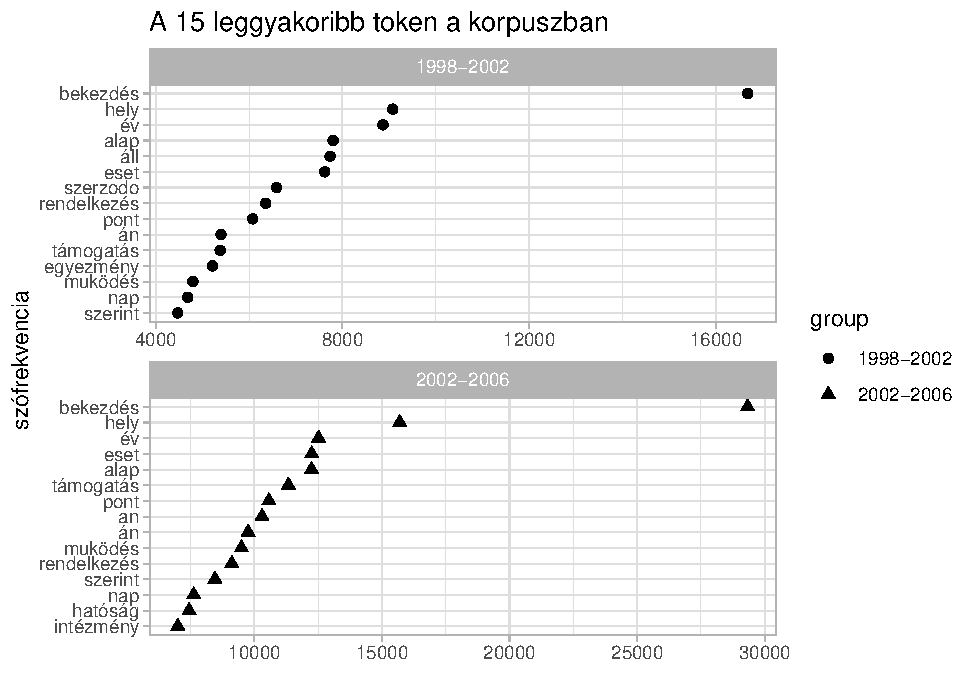
\includegraphics[width=0.9\linewidth]{_main_files/figure-latex/unnamed-chunk-80-1} \end{center}

A szövegtisztító lépéseket később újabbakkal is kiegészíthetjük, ha
észrevesszük, hogy az elemzést zavaró tisztítási lépés maradt ki. Ilyen
esetben tovább tisztíthatjuk a korpuszt, majd újra lefuttathatjuk az
elemzést. Például, ha szükséges, további stopszavak eltávolítását is
elvégezhetjük egy újabb stopszólista hozzáadásával. Ilyenkor ugyanúgy
járunk el, mint az előző stopszólista esetén, vagyis beolvassuk a
munkakönyvtárban elhelyezett a \texttt{csv} fájlt, a beolvasott
stopszólistából karakter vektort majd objektumot hozunk létre, végezetül
pedig ezeket a szavakat is eltávolítjuk a kopuszból.

\begin{Shaded}
\begin{Highlighting}[]
\NormalTok{custom\_stopwords2 }\OtherTok{\textless{}{-}} \FunctionTok{readtext}\NormalTok{(}\StringTok{"data/custom\_stopwords2.csv"}\NormalTok{, }\AttributeTok{encoding =} \StringTok{"UTF8"}\NormalTok{) }\SpecialCharTok{\%\textgreater{}\%}
  \FunctionTok{pull}\NormalTok{(text)}

\NormalTok{torvenyek\_tokens\_final }\OtherTok{\textless{}{-}}\NormalTok{ torvenyek\_tokens }\SpecialCharTok{\%\textgreater{}\%}
  \FunctionTok{tokens\_remove}\NormalTok{(custom\_stopwords2)}
\end{Highlighting}
\end{Shaded}

Ezután újra ellenőrízzük az eredményt.

\begin{Shaded}
\begin{Highlighting}[]
\NormalTok{torvenyek\_dfm\_final }\OtherTok{\textless{}{-}} \FunctionTok{dfm}\NormalTok{(torvenyek\_tokens\_final) }\SpecialCharTok{\%\textgreater{}\%}
  \FunctionTok{dfm\_trim}\NormalTok{(}\AttributeTok{min\_termfreq =} \FloatTok{0.001}\NormalTok{, }\AttributeTok{termfreq\_type =} \StringTok{"prop"}\NormalTok{)}

\NormalTok{top\_tokens\_final }\OtherTok{\textless{}{-}} \FunctionTok{textstat\_frequency}\NormalTok{(torvenyek\_dfm\_final, }\AttributeTok{n =} \DecValTok{15}\NormalTok{, }\AttributeTok{groups =} \FunctionTok{docvars}\NormalTok{(torvenyek\_dfm, }\AttributeTok{field =} \StringTok{"electoral\_cycle"}\NormalTok{))}

\FunctionTok{ggplot}\NormalTok{(top\_tokens\_final, }\FunctionTok{aes}\NormalTok{(}\FunctionTok{reorder\_within}\NormalTok{(feature, frequency, group), frequency)) }\SpecialCharTok{+}
  \FunctionTok{geom\_point}\NormalTok{(}\FunctionTok{aes}\NormalTok{(}\AttributeTok{shape =}\NormalTok{ group), }\AttributeTok{size =} \DecValTok{2}\NormalTok{) }\SpecialCharTok{+}
  \FunctionTok{coord\_flip}\NormalTok{() }\SpecialCharTok{+}
  \FunctionTok{labs}\NormalTok{(}
    \AttributeTok{y =} \ConstantTok{NULL}\NormalTok{,}
    \AttributeTok{x =} \StringTok{"szófrekvencia"}\NormalTok{,}
    \AttributeTok{title =} \StringTok{"A 15 leggyakoribb token a korpuszban"}\NormalTok{,}
    \AttributeTok{subtitle =} \StringTok{"Eredmény a bovített stop szó listával"}
\NormalTok{  ) }\SpecialCharTok{+}
  \FunctionTok{facet\_wrap}\NormalTok{(}\SpecialCharTok{\textasciitilde{}}\NormalTok{group, }\AttributeTok{nrow =} \DecValTok{2}\NormalTok{, }\AttributeTok{scales =} \StringTok{"free"}\NormalTok{) }\SpecialCharTok{+}
\NormalTok{  tidytext}\SpecialCharTok{::}\FunctionTok{scale\_x\_reordered}\NormalTok{()}
\end{Highlighting}
\end{Shaded}

\begin{center}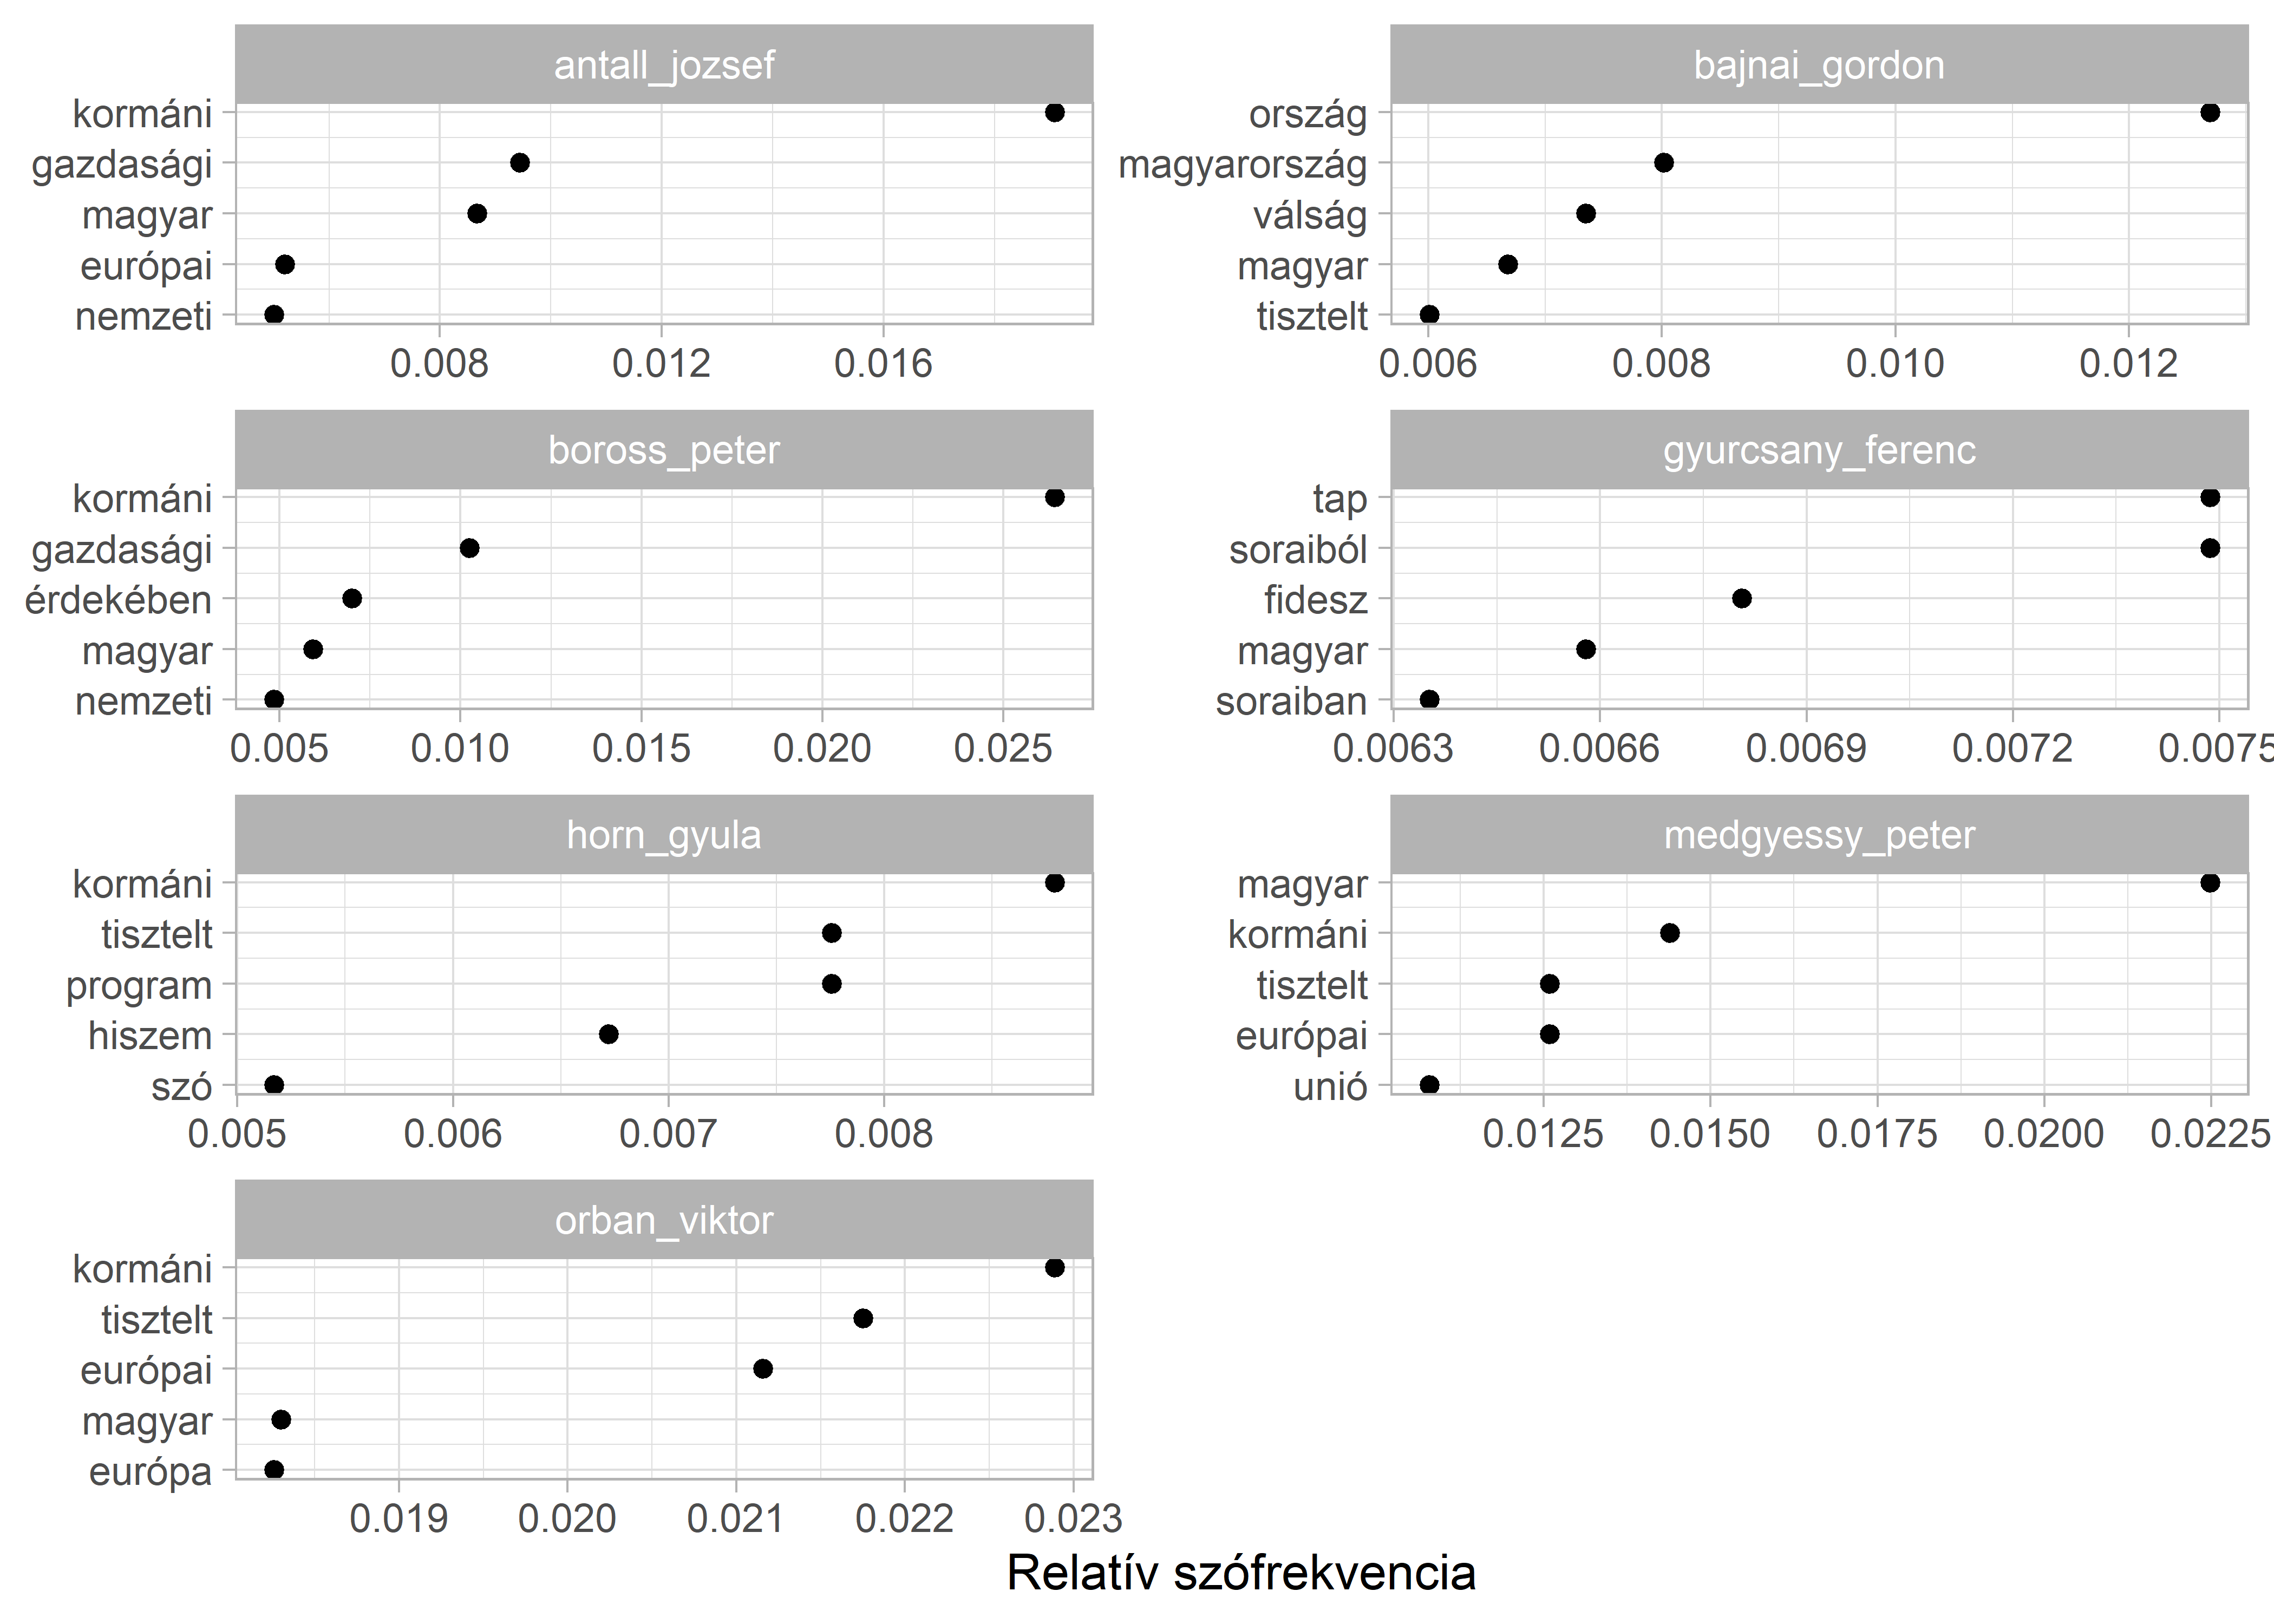
\includegraphics[width=0.9\linewidth]{_main_files/figure-latex/unnamed-chunk-82-1} \end{center}

A szövegtisztító és korpusz előkészítő műveletek után következhet az LDA
illesztése. Az alábbiakban az LDA illesztés két módszerét a
\texttt{VEM}-et és a \texttt{Gibbs}-et mutatjuk be. A modell minkét
módszer esetén ugyanaz, a különbség a következtetés módjában van. A
\texttt{VEM} módszer variációs következtetés, míg a \texttt{Gibbs}
mintavételen alapuló következtetés.
(\protect\hyperlink{ref-blei2003}{\textbf{blei2003?}};
\protect\hyperlink{ref-Griffiths2002}{\textbf{Griffiths2002?}};
\protect\hyperlink{ref-Phan2008}{\textbf{Phan2008?}})

A két modell illesztése nagyon hasonló, meg kell adnunk, az elemezni
kívánt \texttt{dfm} nevét, majd a \emph{„k"} értékét, ami egyenlő az
általunk létrehozni kívánt topikok számával, ezt követően meg kell
jelölnünk, hogy a \texttt{VEM} vagy a \texttt{Gibbs} módszert
alkalmazzuk. A \texttt{set.seed()} a funkció az R véletlen szám
generátor magjának beállítására szolgál, ami ahhoz kell, hogy az
eredmény, ábra, stb. pontosan reprodukálható legyen. A
\texttt{set.seed()} bármilyen tetszőleges egész szám lehet.
Kihasználhatjuk hogy minden dokumentumhoz tartozik egy kormányzati
ciklus azonosító, mivel ésszerű lehet a feltételezés, hogy különböző
parlamentek és kormányok más-más jogalkotási fokusszal rendelkeznek. A
dokumentum változók alapján a \texttt{dfm\_subset()}-el tudjuk
feldarabolni a már elkészült és tisztított mátrixunkat.

\begin{Shaded}
\begin{Highlighting}[]
\NormalTok{dfm\_98\_02 }\OtherTok{\textless{}{-}} \FunctionTok{dfm\_subset}\NormalTok{(torvenyek\_dfm\_final, electoral\_cycle }\SpecialCharTok{==} \StringTok{"1998{-}2002"}\NormalTok{)}

\NormalTok{dfm\_02\_06 }\OtherTok{\textless{}{-}} \FunctionTok{dfm\_subset}\NormalTok{(torvenyek\_dfm\_final, electoral\_cycle }\SpecialCharTok{==} \StringTok{"2002{-}2006"}\NormalTok{)}
\end{Highlighting}
\end{Shaded}

\hypertarget{a-vem-muxf3dszer-alkalmazuxe1sa-a-magyar-tuxf6rvuxe9nyek-korpuszuxe1n}{%
\subsection{A „VEM" módszer alkalmazása a magyar törvények
korpuszán}\label{a-vem-muxf3dszer-alkalmazuxe1sa-a-magyar-tuxf6rvuxe9nyek-korpuszuxe1n}}

Saját korpuszunkon először a \texttt{VEM} a módszert alkalmazzuk, ahol
\texttt{k\ =\ 10} azaz a modell 10 témacsoportot alakít ki. Mint arról
korábban már volt szó a \texttt{k} értékét szabadon változtathatjuk,
aszerint hogy hány topik kialakítását szeretnénk. Bár a \texttt{k}
értékének meghatározása kutatói döntésen alapul, és a modell futtatása
során bevett gyakorlat a különböző \emph{„k"} értékekkel való
kísérletezés, miután elkészült az elemzés a \texttt{perplexity()}
funkció segítségével -- ahol a \emph{theta} az adott topikhoz való
tartozás valószínűsége -- lehetőségünk van az elkészült modell
kiértékelésére. A függvény a topikok által reprezentált elméleti
szóeloszlásokat hasonlítja össze a szavak tényleges eloszlásával a
dokumentumokban. A függvény értéke nem önmagában értelmezendő, hanem két
modell összehasonlításában, ahol a legalacsonyabb \emph{perplexity}
(zavarodottság) értékkel rendelkező modellt tekintik a
legjobbnak.{[}\^{}klaszeterzes-2{]} Az illusztráció kedvéért
lefuttatunk5 LDA modellt az 1998-2002 kormánzyati ciklushoz tartozó
dfm-en. Az iterációhoz a \texttt{purrr} csomag \texttt{map} függvényét
használjuk (ez a \texttt{lapply} \emph{tidyverse} ekvivalense). Fontos
emlékezni arra, hogy minél nagyobb a korpuszunk annál több számítási
kapacitásra van szükség (és annál tovább tart a számítás).

{[}\^{}klaszeterzes-2{]}
\url{http://brooksandrew.github.io/simpleblog/articles/latent-dirichlet-allocation-under-the-hood/}

\begin{Shaded}
\begin{Highlighting}[]
\FunctionTok{library}\NormalTok{(purrr)}
\end{Highlighting}
\end{Shaded}

\begin{Shaded}
\begin{Highlighting}[]
\NormalTok{k\_topics }\OtherTok{\textless{}{-}} \FunctionTok{c}\NormalTok{(}\DecValTok{5}\NormalTok{, }\DecValTok{10}\NormalTok{, }\DecValTok{15}\NormalTok{, }\DecValTok{20}\NormalTok{, }\DecValTok{25}\NormalTok{)}

\NormalTok{lda\_98\_02 }\OtherTok{\textless{}{-}}\NormalTok{ k\_topics }\SpecialCharTok{\%\textgreater{}\%}
  \FunctionTok{map}\NormalTok{(LDA, }\AttributeTok{x =}\NormalTok{ dfm\_98\_02, }\AttributeTok{control =} \FunctionTok{list}\NormalTok{(}\AttributeTok{seed =} \DecValTok{1234}\NormalTok{))}


\FunctionTok{tibble}\NormalTok{(}
  \AttributeTok{k =}\NormalTok{ k\_topics,}
  \AttributeTok{perplexity =} \FunctionTok{map\_dbl}\NormalTok{(lda\_98\_02, perplexity)}
\NormalTok{) }\SpecialCharTok{\%\textgreater{}\%}
  \FunctionTok{ggplot}\NormalTok{(}\FunctionTok{aes}\NormalTok{(k, perplexity)) }\SpecialCharTok{+}
  \FunctionTok{geom\_point}\NormalTok{() }\SpecialCharTok{+}
  \FunctionTok{geom\_line}\NormalTok{() }\SpecialCharTok{+}
  \FunctionTok{labs}\NormalTok{(}
    \AttributeTok{title =} \StringTok{"Mekkora k?"}\NormalTok{,}
    \AttributeTok{subtitle =} \StringTok{"Perplexity változása a k függvényében"}\NormalTok{,}
    \AttributeTok{x =} \StringTok{"k"}\NormalTok{,}
    \AttributeTok{y =} \StringTok{"Perplexity"}
\NormalTok{  )}
\end{Highlighting}
\end{Shaded}

\begin{center}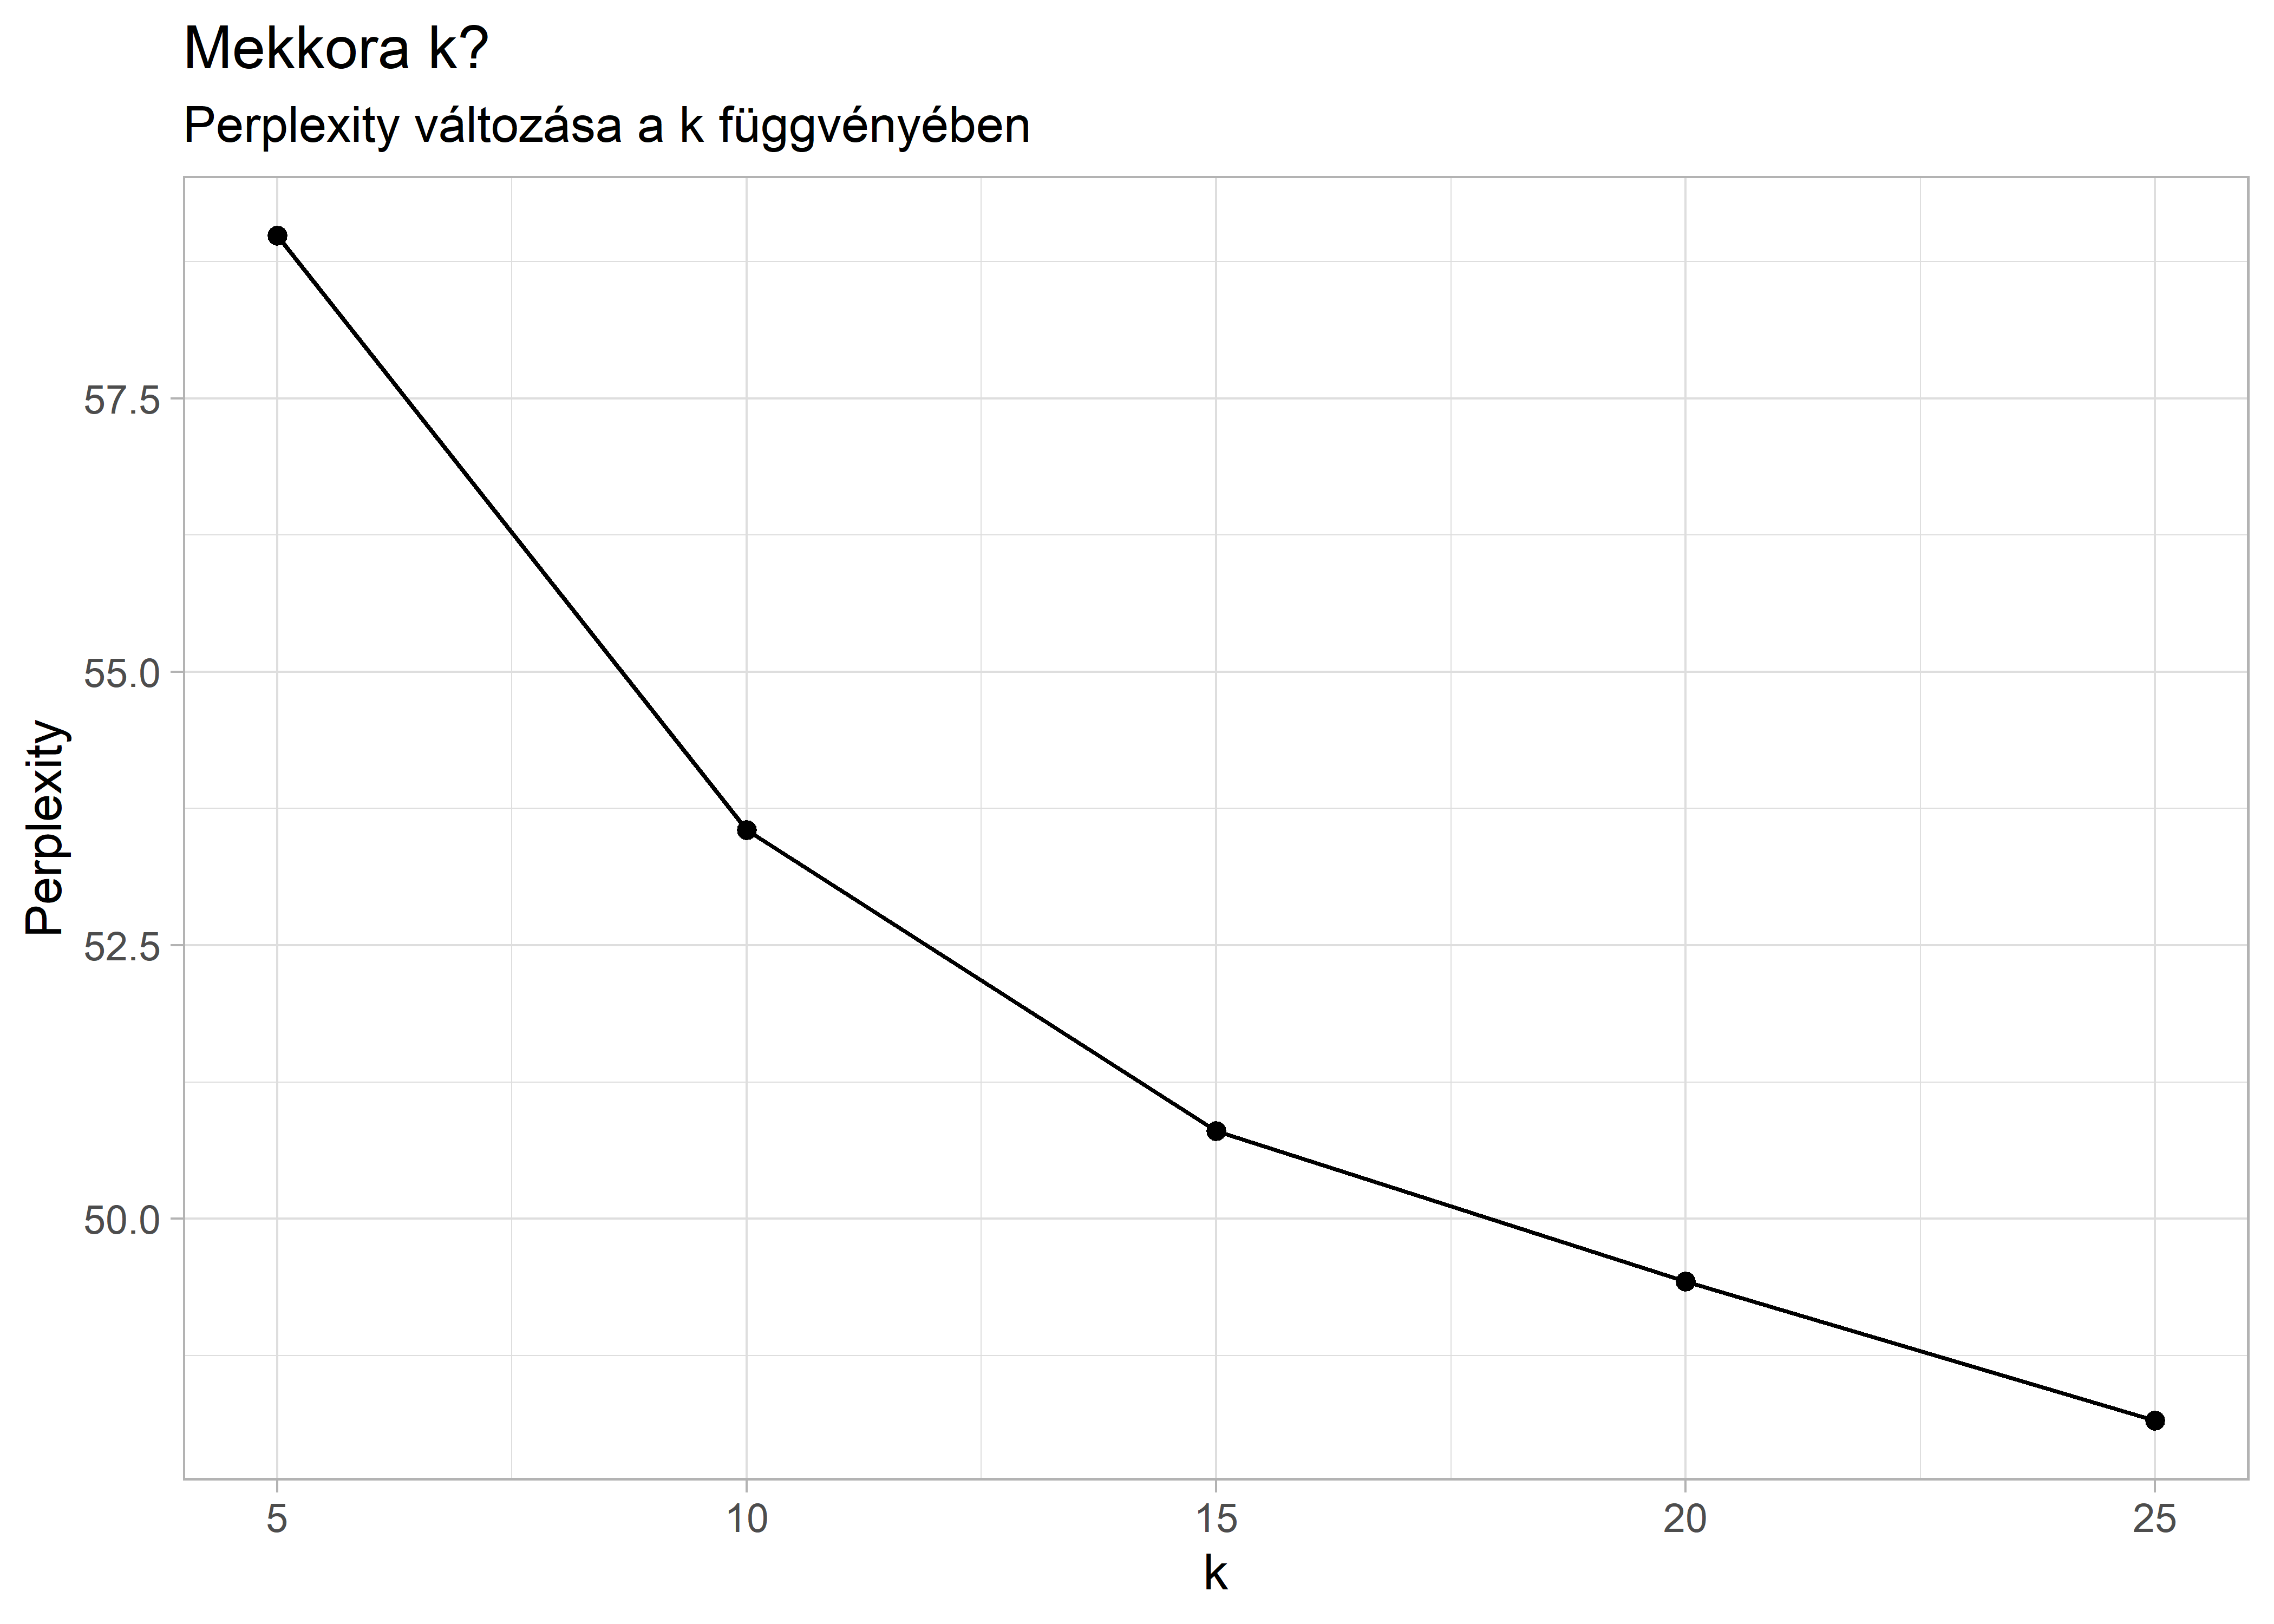
\includegraphics[width=0.9\linewidth]{_main_files/figure-latex/unnamed-chunk-85-1} \end{center}

A perplexity pontszám alapján a 25 topikos modell szerepel a legjobban,
de fontos emlékezni arra hogy a megfelelő \emph{k} kiválasztása a kutató
kvalitatív döntésén múlik. Ehhez természetesen kvantitatív szempontokat
is figyelembe vehetünk, mint például a perplexity indikátor.\footnote{A
  \texttt{ldatuning} R csomagban további indikátor implementációja
  található, ami a perplexityhez hasonlóan minimalizásra alapoz
  (\protect\hyperlink{ref-arun2010finding}{Arun et al.}
  (\protect\hyperlink{ref-arun2010finding}{2010}),
  \protect\hyperlink{ref-cao2009density}{Cao et al.}
  (\protect\hyperlink{ref-cao2009density}{2009})), illetve
  maximalizálásra (\protect\hyperlink{ref-deveaud2014accurate}{Deveaud,
  SanJuan, and Bellot}
  (\protect\hyperlink{ref-deveaud2014accurate}{2014}),
  \protect\hyperlink{ref-griffiths2004}{Griffiths and Steyvers}
  (\protect\hyperlink{ref-griffiths2004}{2004}))}

A reprodukálhatóság és futási sebesség érdekében a fejezet további
részeiben a \emph{k} paraméternek 10-es értéket adunk. Ezzel
lefututtatunk egy-egy modellt a két ciklusra.

\begin{Shaded}
\begin{Highlighting}[]
\NormalTok{vem\_98\_02 }\OtherTok{\textless{}{-}} \FunctionTok{LDA}\NormalTok{(dfm\_98\_02, }\AttributeTok{k =} \DecValTok{10}\NormalTok{, }\AttributeTok{method =} \StringTok{"VEM"}\NormalTok{, }\AttributeTok{control =} \FunctionTok{list}\NormalTok{(}\AttributeTok{seed =} \DecValTok{1234}\NormalTok{))}

\NormalTok{vem\_02\_06 }\OtherTok{\textless{}{-}} \FunctionTok{LDA}\NormalTok{(dfm\_02\_06, }\AttributeTok{k =} \DecValTok{10}\NormalTok{, }\AttributeTok{method =} \StringTok{"VEM"}\NormalTok{, }\AttributeTok{control =} \FunctionTok{list}\NormalTok{(}\AttributeTok{seed =} \DecValTok{1234}\NormalTok{))}
\end{Highlighting}
\end{Shaded}

Ezt követően a modell által létrehozott topic-okat tidy formátumba
tesszük és egyesítjük egy data frameben.\footnote{a tidy formátumról
  bővebben:
  \url{https://cran.r-project.org/web/packages/tidyr/vignettes/tidy-data.html}}

\begin{Shaded}
\begin{Highlighting}[]
\FunctionTok{library}\NormalTok{(tidytext)}
\end{Highlighting}
\end{Shaded}

\begin{Shaded}
\begin{Highlighting}[]
\NormalTok{topics\_98\_02 }\OtherTok{\textless{}{-}} \FunctionTok{tidy}\NormalTok{(vem\_98\_02, }\AttributeTok{matrix =} \StringTok{"beta"}\NormalTok{) }\SpecialCharTok{\%\textgreater{}\%}
  \FunctionTok{mutate}\NormalTok{(}\AttributeTok{electoral\_cycle =} \StringTok{"1998{-}2002"}\NormalTok{)}

\NormalTok{topics\_02\_06 }\OtherTok{\textless{}{-}} \FunctionTok{tidy}\NormalTok{(vem\_02\_06, }\AttributeTok{matrix =} \StringTok{"beta"}\NormalTok{) }\SpecialCharTok{\%\textgreater{}\%}
  \FunctionTok{mutate}\NormalTok{(}\AttributeTok{electoral\_cycle =} \StringTok{"2002{-}2006"}\NormalTok{)}

\NormalTok{lda\_vem }\OtherTok{\textless{}{-}} \FunctionTok{bind\_rows}\NormalTok{(topics\_98\_02, topics\_02\_06)}
\end{Highlighting}
\end{Shaded}

Majd listázzuk az egyes topikokhoz tartozó leggyakoribb kifejezéseket.

\begin{Shaded}
\begin{Highlighting}[]

\NormalTok{top\_terms }\OtherTok{\textless{}{-}}\NormalTok{ lda\_vem }\SpecialCharTok{\%\textgreater{}\%}
  \FunctionTok{group\_by}\NormalTok{(electoral\_cycle, topic) }\SpecialCharTok{\%\textgreater{}\%}
  \FunctionTok{top\_n}\NormalTok{(}\DecValTok{5}\NormalTok{, beta) }\SpecialCharTok{\%\textgreater{}\%}
  \FunctionTok{top\_n}\NormalTok{(}\DecValTok{5}\NormalTok{, term) }\SpecialCharTok{\%\textgreater{}\%}
  \FunctionTok{ungroup}\NormalTok{() }\SpecialCharTok{\%\textgreater{}\%}
  \FunctionTok{arrange}\NormalTok{(topic, }\SpecialCharTok{{-}}\NormalTok{beta)}
\end{Highlighting}
\end{Shaded}

Majd a \texttt{ggplot2} csomag segítségével ábrán is megjeleníthetjük az
egyes topikok 10 legfontosabb kifejezését.

\begin{Shaded}
\begin{Highlighting}[]
\NormalTok{top\_terms }\SpecialCharTok{\%\textgreater{}\%}
  \FunctionTok{filter}\NormalTok{(electoral\_cycle }\SpecialCharTok{==} \StringTok{"1998{-}2002"}\NormalTok{) }\SpecialCharTok{\%\textgreater{}\%}
  \FunctionTok{ggplot}\NormalTok{(}\FunctionTok{aes}\NormalTok{(}\FunctionTok{reorder\_within}\NormalTok{(term, beta, topic), beta)) }\SpecialCharTok{+}
  \FunctionTok{geom\_col}\NormalTok{(}\AttributeTok{show.legend =} \ConstantTok{FALSE}\NormalTok{) }\SpecialCharTok{+}
  \FunctionTok{facet\_wrap}\NormalTok{(}\SpecialCharTok{\textasciitilde{}}\NormalTok{topic, }\AttributeTok{scales =} \StringTok{"free"}\NormalTok{, }\AttributeTok{ncol =} \DecValTok{2}\NormalTok{) }\SpecialCharTok{+}
  \FunctionTok{coord\_flip}\NormalTok{() }\SpecialCharTok{+}
  \FunctionTok{labs}\NormalTok{(}
    \AttributeTok{title =} \StringTok{"1998{-}2002 ciklus topikok és kifejezések"}\NormalTok{,}
    \AttributeTok{x =} \ConstantTok{NULL}\NormalTok{,}
    \AttributeTok{y =} \FunctionTok{expression}\NormalTok{(beta)}
\NormalTok{  ) }\SpecialCharTok{+}
\NormalTok{  tidytext}\SpecialCharTok{::}\FunctionTok{scale\_x\_reordered}\NormalTok{()}
\end{Highlighting}
\end{Shaded}

\begin{center}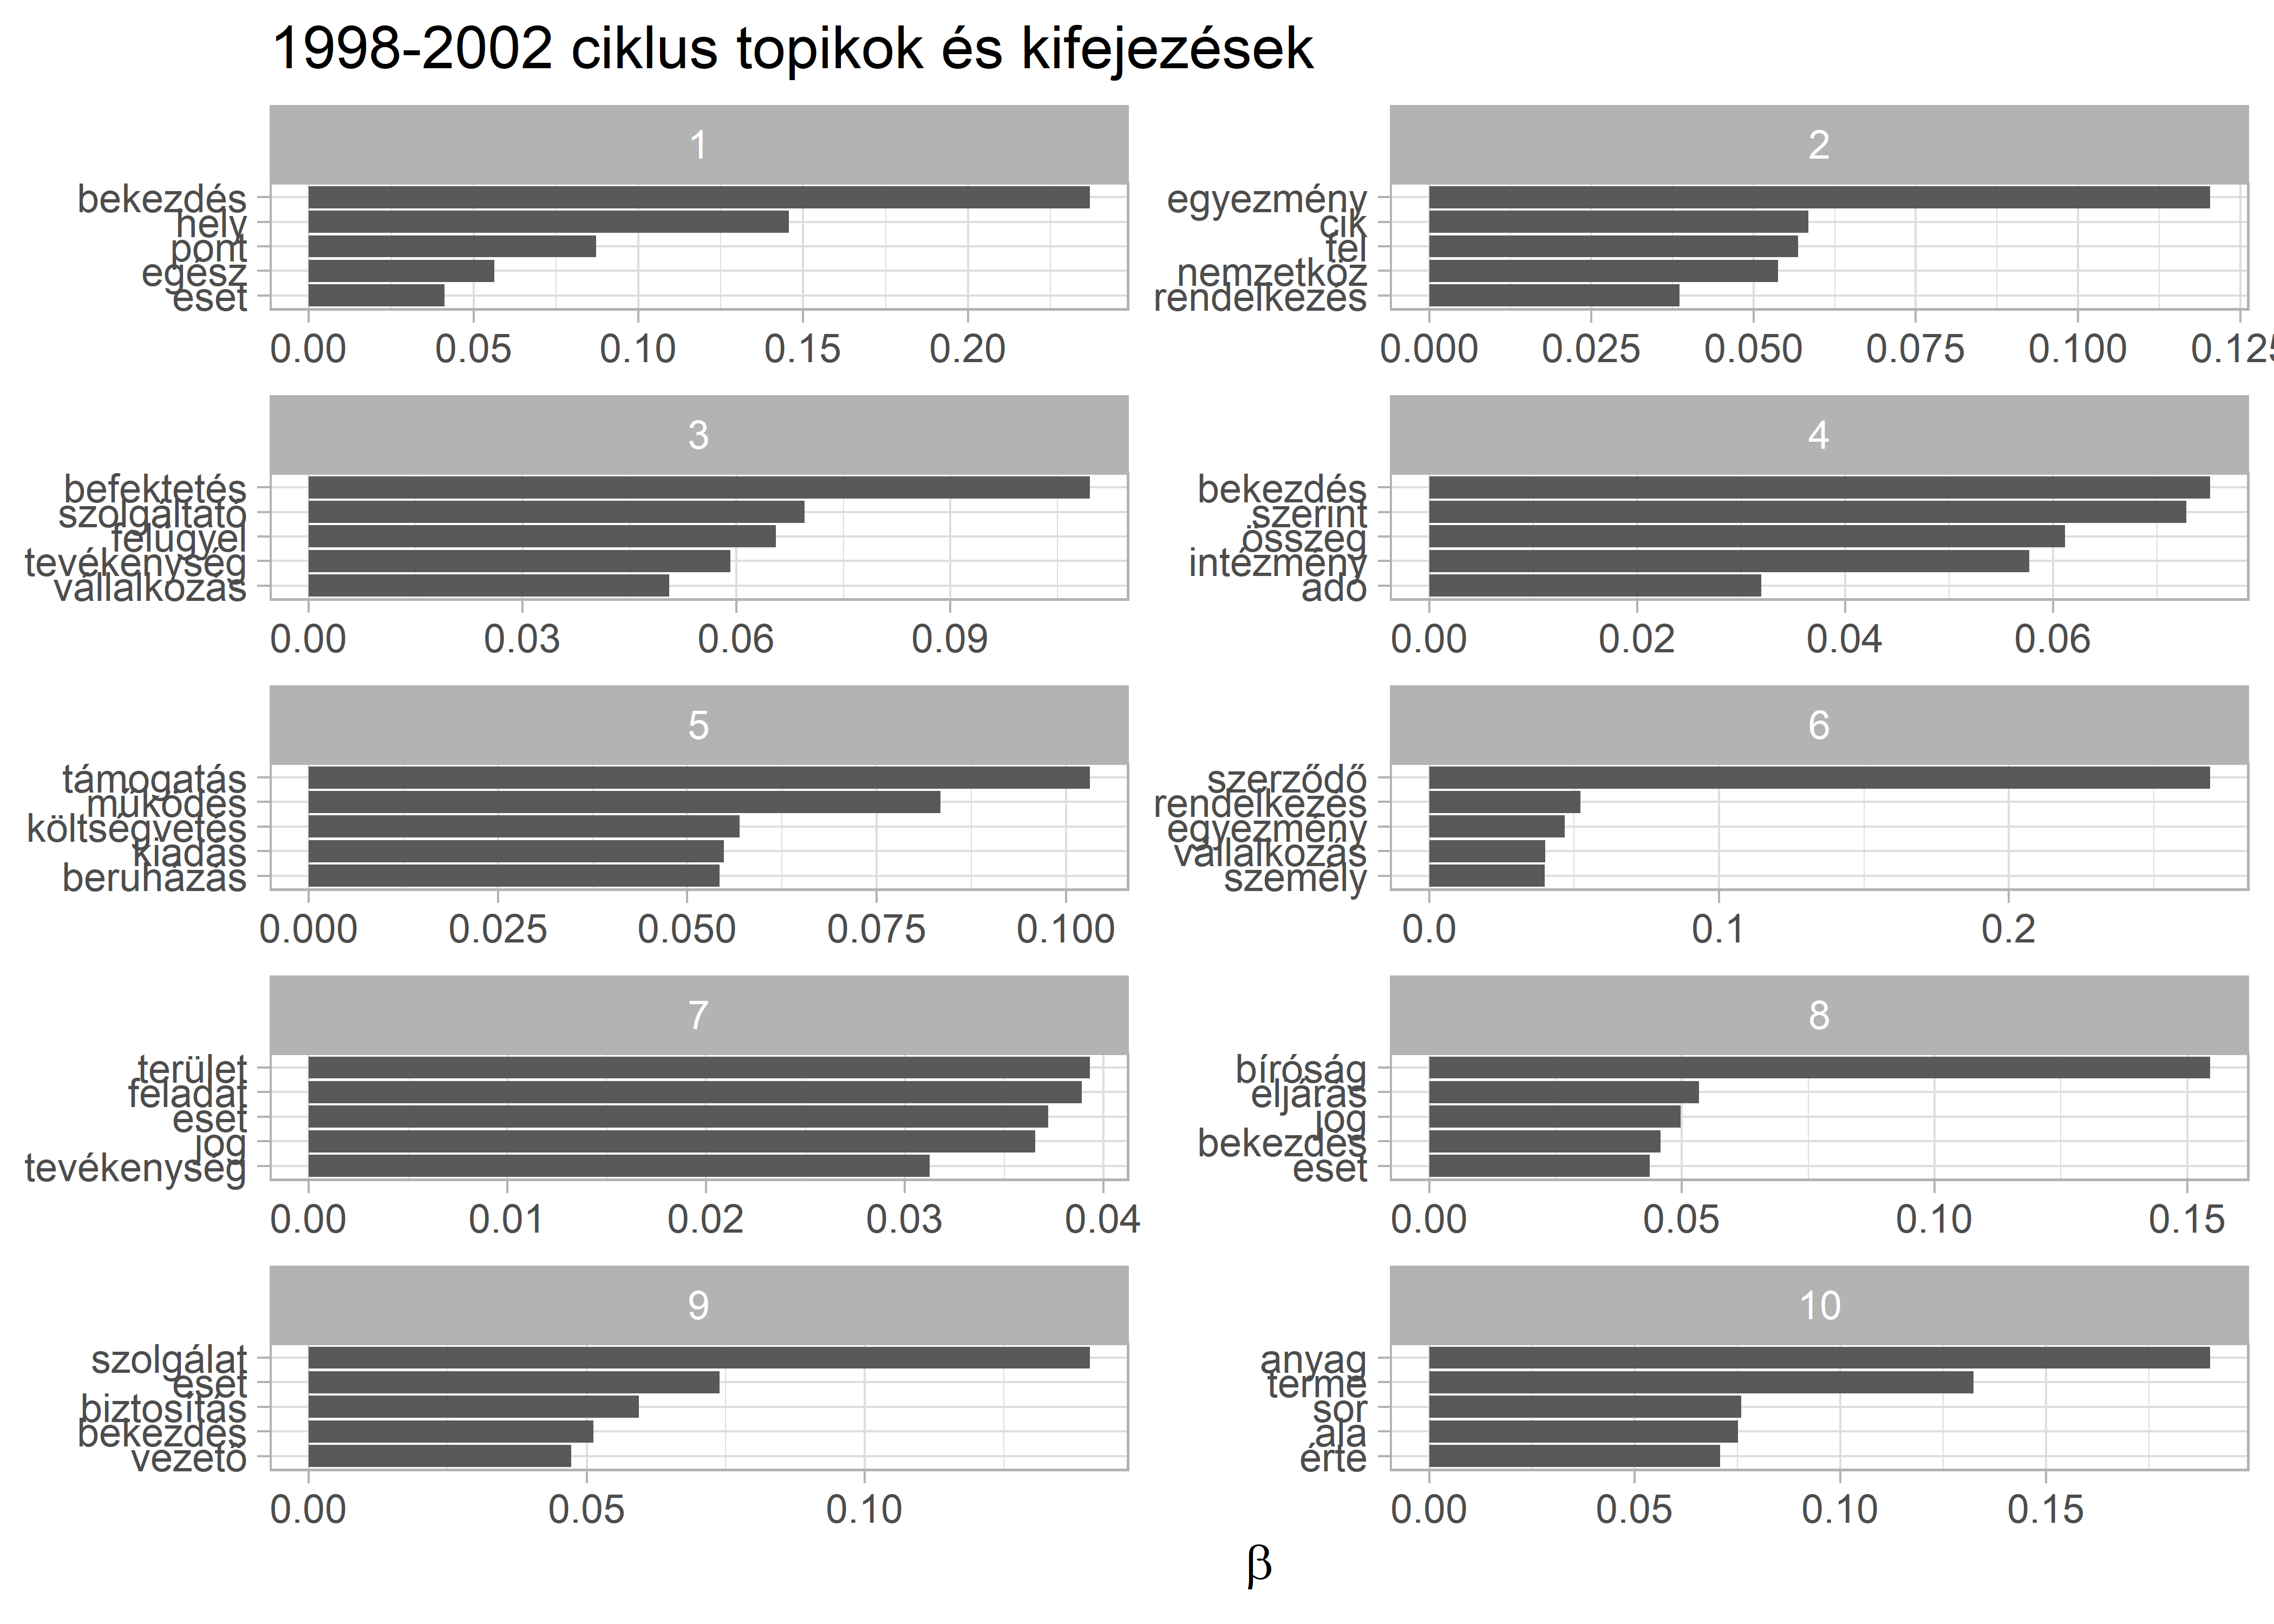
\includegraphics[width=0.9\linewidth]{_main_files/figure-latex/unnamed-chunk-90-1} \end{center}

\begin{Shaded}
\begin{Highlighting}[]
\NormalTok{top\_terms }\SpecialCharTok{\%\textgreater{}\%}
  \FunctionTok{filter}\NormalTok{(electoral\_cycle }\SpecialCharTok{==} \StringTok{"2002{-}2006"}\NormalTok{) }\SpecialCharTok{\%\textgreater{}\%}
  \FunctionTok{ggplot}\NormalTok{(}\FunctionTok{aes}\NormalTok{(}\FunctionTok{reorder\_within}\NormalTok{(term, beta, topic), beta)) }\SpecialCharTok{+}
  \FunctionTok{geom\_col}\NormalTok{(}\AttributeTok{show.legend =} \ConstantTok{FALSE}\NormalTok{) }\SpecialCharTok{+}
  \FunctionTok{facet\_wrap}\NormalTok{(}\SpecialCharTok{\textasciitilde{}}\NormalTok{topic, }\AttributeTok{scales =} \StringTok{"free"}\NormalTok{, }\AttributeTok{ncol =} \DecValTok{2}\NormalTok{) }\SpecialCharTok{+}
  \FunctionTok{coord\_flip}\NormalTok{() }\SpecialCharTok{+}
  \FunctionTok{labs}\NormalTok{(}
    \AttributeTok{title =} \StringTok{"2002{-}2006 ciklus topikok és kifejezések"}\NormalTok{,}
    \AttributeTok{x =} \ConstantTok{NULL}\NormalTok{,}
    \AttributeTok{y =} \FunctionTok{expression}\NormalTok{(beta)}
\NormalTok{  ) }\SpecialCharTok{+}
\NormalTok{  tidytext}\SpecialCharTok{::}\FunctionTok{scale\_x\_reordered}\NormalTok{()}
\end{Highlighting}
\end{Shaded}

\begin{center}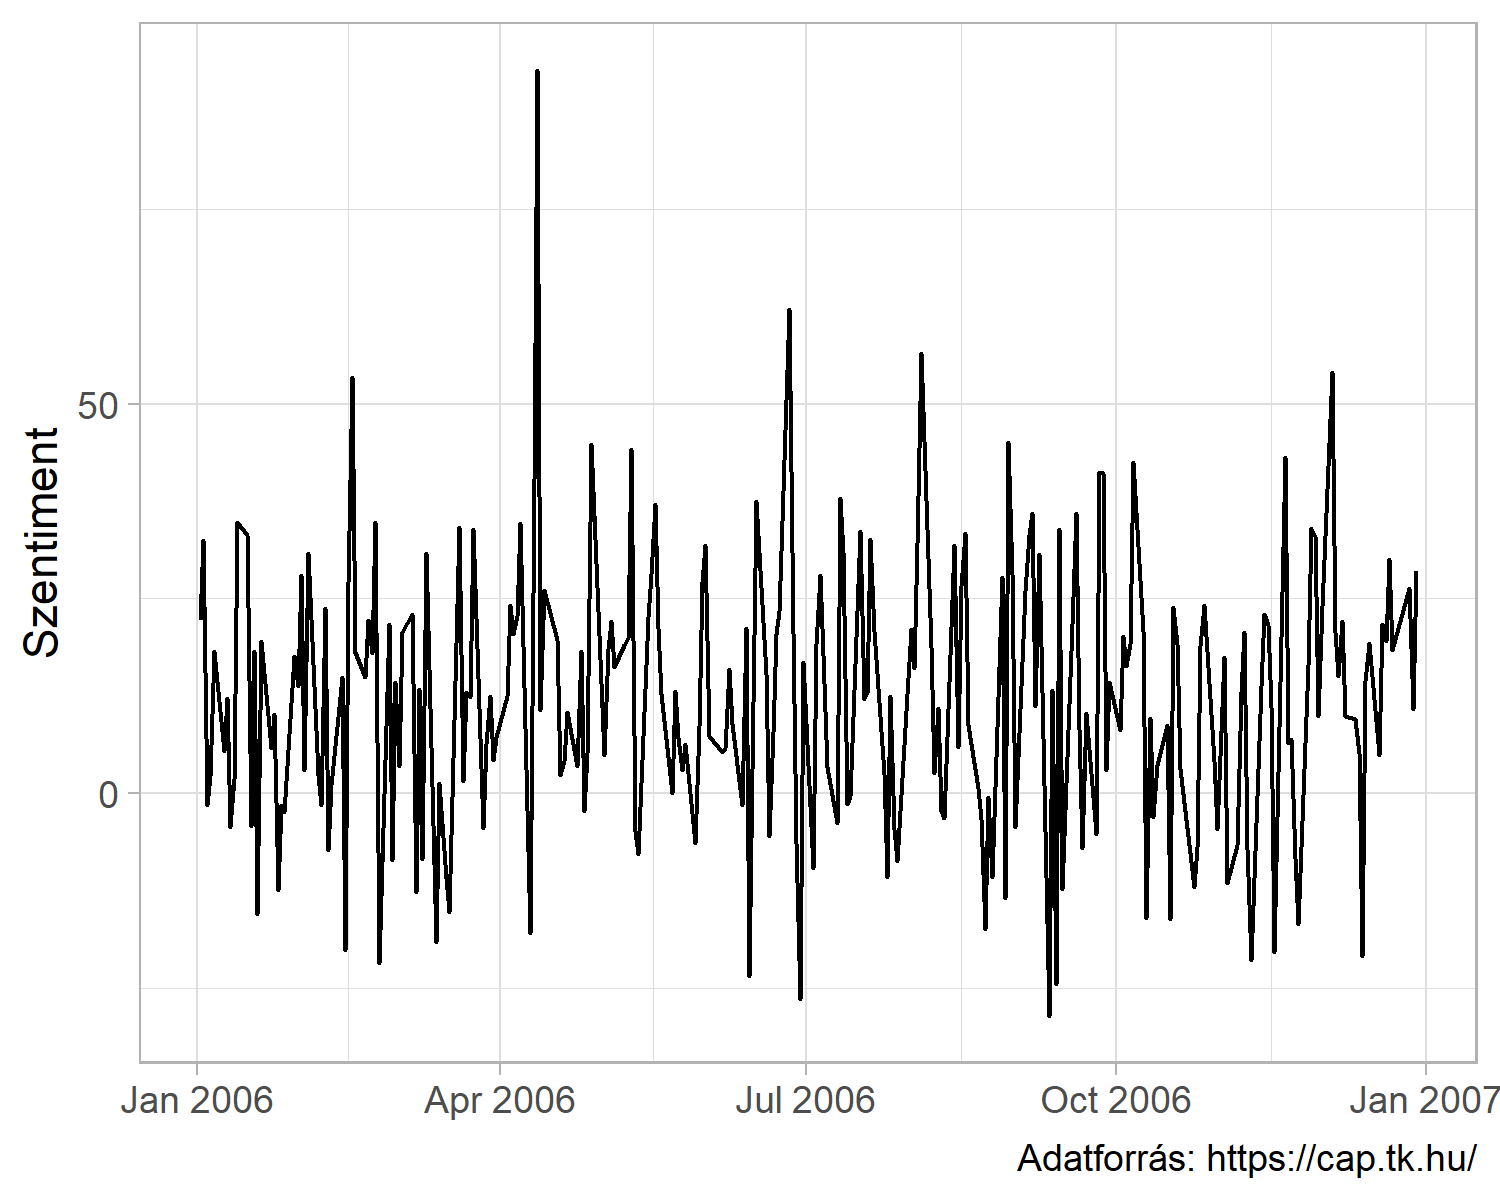
\includegraphics[width=0.9\linewidth]{_main_files/figure-latex/unnamed-chunk-91-1} \end{center}

\hypertarget{az-lda-gibbs-muxf3dszer-alkalmazuxe1sa-a-magyar-tuxf6rvuxe9nyek-korpuszuxe1n}{%
\subsection{Az „LDA Gibbs" módszer alkalmazása a magyar törvények
korpuszán}\label{az-lda-gibbs-muxf3dszer-alkalmazuxe1sa-a-magyar-tuxf6rvuxe9nyek-korpuszuxe1n}}

A következőkben ugyanazon a korpuszon az LDA Gibbs módszert alkalmazzuk.
A szövegelőkészítő és tisztító lépések ennél a módszernél is ugyanazok
mint a fentebb bemutatott ``VEM'' módszer esetében, így itt most csak a
modell illesztését mutatjuk be.

\begin{Shaded}
\begin{Highlighting}[]

\NormalTok{gibbs\_98\_02 }\OtherTok{\textless{}{-}} \FunctionTok{LDA}\NormalTok{(dfm\_98\_02, }\AttributeTok{k =} \DecValTok{10}\NormalTok{, }\AttributeTok{method =} \StringTok{"Gibbs"}\NormalTok{, }\AttributeTok{control =} \FunctionTok{list}\NormalTok{(}\AttributeTok{seed =} \DecValTok{1234}\NormalTok{))}

\NormalTok{gibbs\_02\_06 }\OtherTok{\textless{}{-}} \FunctionTok{LDA}\NormalTok{(dfm\_02\_06, }\AttributeTok{k =} \DecValTok{10}\NormalTok{, }\AttributeTok{method =} \StringTok{"Gibbs"}\NormalTok{, }\AttributeTok{control =} \FunctionTok{list}\NormalTok{(}\AttributeTok{seed =} \DecValTok{1234}\NormalTok{))}
\end{Highlighting}
\end{Shaded}

Itt is elvégezzük a topikok tidy formátumra alakítását.

\begin{Shaded}
\begin{Highlighting}[]
\NormalTok{topics\_g98\_02 }\OtherTok{\textless{}{-}} \FunctionTok{tidy}\NormalTok{(gibbs\_98\_02, }\AttributeTok{matrix =} \StringTok{"beta"}\NormalTok{) }\SpecialCharTok{\%\textgreater{}\%}
  \FunctionTok{mutate}\NormalTok{(}\AttributeTok{electoral\_cycle =} \StringTok{"1998{-}2002"}\NormalTok{)}

\NormalTok{topics\_g02\_06 }\OtherTok{\textless{}{-}} \FunctionTok{tidy}\NormalTok{(gibbs\_02\_06, }\AttributeTok{matrix =} \StringTok{"beta"}\NormalTok{) }\SpecialCharTok{\%\textgreater{}\%}
  \FunctionTok{mutate}\NormalTok{(}\AttributeTok{electoral\_cycle =} \StringTok{"2002{-}2006"}\NormalTok{)}

\NormalTok{lda\_gibbs }\OtherTok{\textless{}{-}} \FunctionTok{bind\_rows}\NormalTok{(topics\_g98\_02, topics\_g02\_06)}
\end{Highlighting}
\end{Shaded}

Majd listázzuk az egyes topikokhoz tartozó leggyakoribb kifejezéseket.

\begin{Shaded}
\begin{Highlighting}[]
\NormalTok{top\_terms\_gibbs }\OtherTok{\textless{}{-}}\NormalTok{ lda\_gibbs }\SpecialCharTok{\%\textgreater{}\%}
  \FunctionTok{group\_by}\NormalTok{(electoral\_cycle, topic) }\SpecialCharTok{\%\textgreater{}\%}
  \FunctionTok{top\_n}\NormalTok{(}\DecValTok{5}\NormalTok{, beta) }\SpecialCharTok{\%\textgreater{}\%}
  \FunctionTok{top\_n}\NormalTok{(}\DecValTok{5}\NormalTok{, term) }\SpecialCharTok{\%\textgreater{}\%}
  \FunctionTok{ungroup}\NormalTok{() }\SpecialCharTok{\%\textgreater{}\%}
  \FunctionTok{arrange}\NormalTok{(topic, }\SpecialCharTok{{-}}\NormalTok{beta)}
\end{Highlighting}
\end{Shaded}

Majd a \texttt{ggplot2} csomag segítségével ábrán is megjeleníthetjük.

\begin{Shaded}
\begin{Highlighting}[]
\NormalTok{top\_terms\_gibbs }\SpecialCharTok{\%\textgreater{}\%}
  \FunctionTok{filter}\NormalTok{(electoral\_cycle }\SpecialCharTok{==} \StringTok{"1998{-}2002"}\NormalTok{) }\SpecialCharTok{\%\textgreater{}\%}
  \FunctionTok{ggplot}\NormalTok{(}\FunctionTok{aes}\NormalTok{(}\FunctionTok{reorder\_within}\NormalTok{(term, beta, topic), beta)) }\SpecialCharTok{+}
  \FunctionTok{geom\_col}\NormalTok{(}\AttributeTok{show.legend =} \ConstantTok{FALSE}\NormalTok{) }\SpecialCharTok{+}
  \FunctionTok{facet\_wrap}\NormalTok{(}\SpecialCharTok{\textasciitilde{}}\NormalTok{topic, }\AttributeTok{scales =} \StringTok{"free"}\NormalTok{, }\AttributeTok{ncol =} \DecValTok{2}\NormalTok{) }\SpecialCharTok{+}
  \FunctionTok{coord\_flip}\NormalTok{() }\SpecialCharTok{+}
  \FunctionTok{labs}\NormalTok{(}
    \AttributeTok{title =} \StringTok{"1998{-}2002 ciklus topikok és kifejezések"}\NormalTok{,}
    \AttributeTok{x =} \ConstantTok{NULL}\NormalTok{,}
    \AttributeTok{y =} \FunctionTok{expression}\NormalTok{(beta)}
\NormalTok{  ) }\SpecialCharTok{+}
\NormalTok{  tidytext}\SpecialCharTok{::}\FunctionTok{scale\_x\_reordered}\NormalTok{()}
\end{Highlighting}
\end{Shaded}

\begin{center}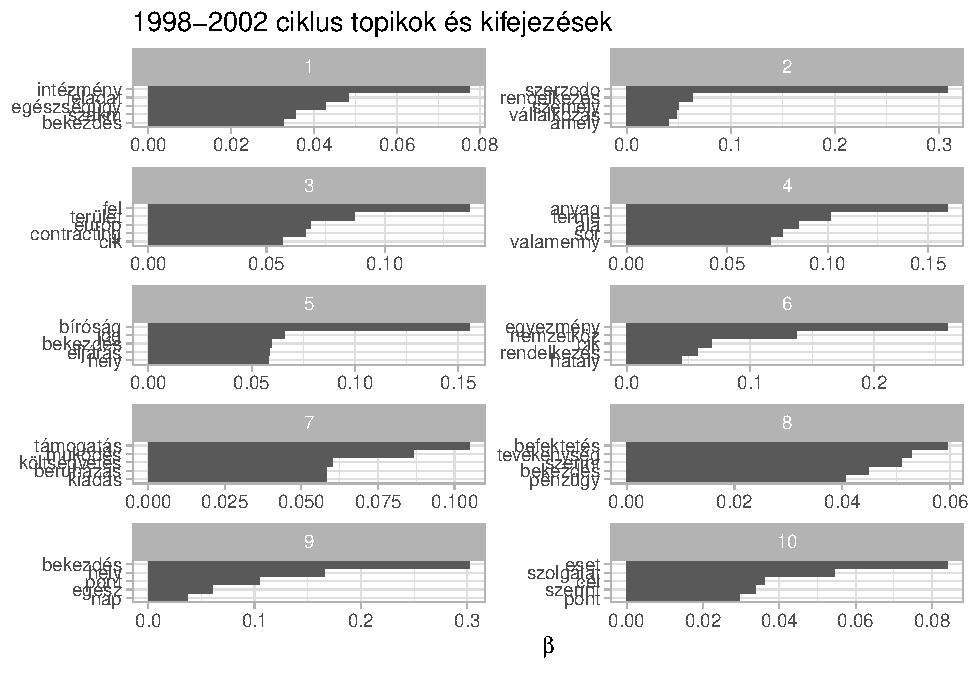
\includegraphics[width=0.9\linewidth]{_main_files/figure-latex/unnamed-chunk-95-1} \end{center}

\begin{Shaded}
\begin{Highlighting}[]
\NormalTok{top\_terms\_gibbs }\SpecialCharTok{\%\textgreater{}\%}
  \FunctionTok{filter}\NormalTok{(electoral\_cycle }\SpecialCharTok{==} \StringTok{"2002{-}2006"}\NormalTok{) }\SpecialCharTok{\%\textgreater{}\%}
  \FunctionTok{ggplot}\NormalTok{(}\FunctionTok{aes}\NormalTok{(}\FunctionTok{reorder\_within}\NormalTok{(term, beta, topic), beta)) }\SpecialCharTok{+}
  \FunctionTok{geom\_col}\NormalTok{(}\AttributeTok{show.legend =} \ConstantTok{FALSE}\NormalTok{) }\SpecialCharTok{+}
  \FunctionTok{facet\_wrap}\NormalTok{(}\SpecialCharTok{\textasciitilde{}}\NormalTok{topic, }\AttributeTok{scales =} \StringTok{"free"}\NormalTok{, }\AttributeTok{ncol =} \DecValTok{2}\NormalTok{) }\SpecialCharTok{+}
  \FunctionTok{coord\_flip}\NormalTok{() }\SpecialCharTok{+}
  \FunctionTok{labs}\NormalTok{(}
    \AttributeTok{title =} \StringTok{"2002{-}2006 ciklus topikok és kifejezések"}\NormalTok{,}
    \AttributeTok{x =} \ConstantTok{NULL}\NormalTok{,}
    \AttributeTok{y =} \FunctionTok{expression}\NormalTok{(beta)}
\NormalTok{  ) }\SpecialCharTok{+}
  \FunctionTok{scale\_x\_reordered}\NormalTok{()}
\end{Highlighting}
\end{Shaded}

\begin{center}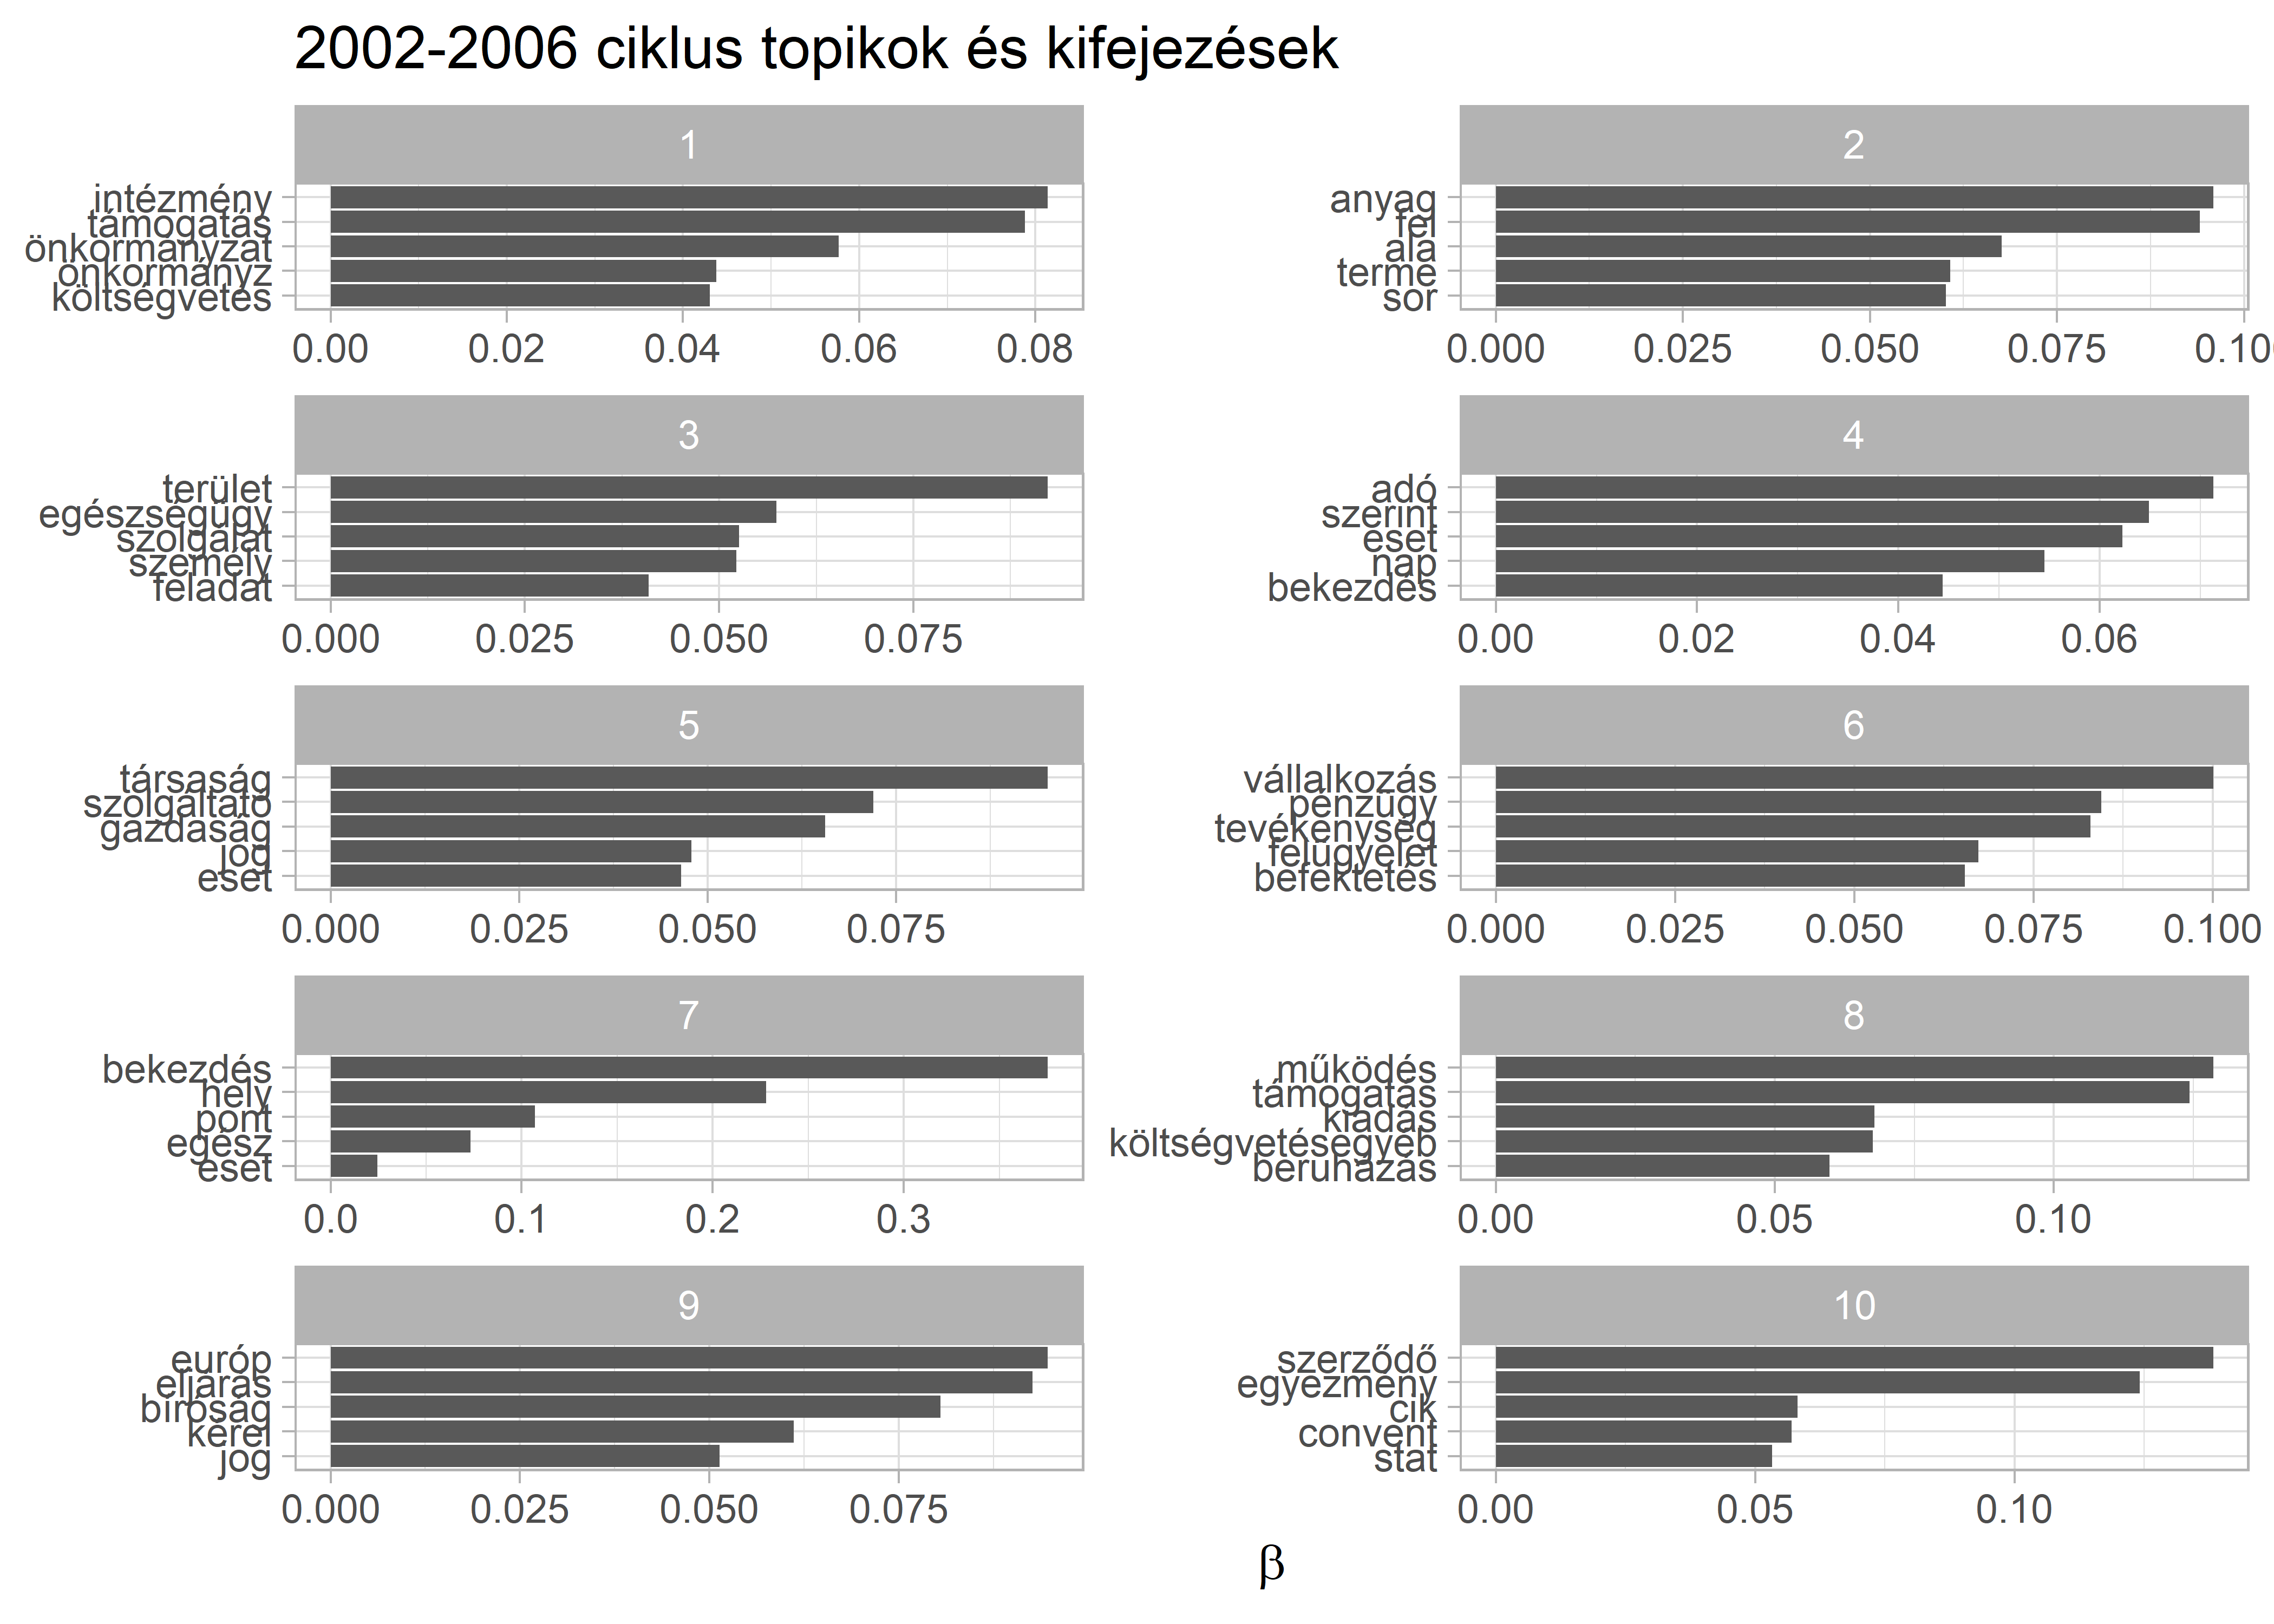
\includegraphics[width=0.9\linewidth]{_main_files/figure-latex/unnamed-chunk-96-1} \end{center}

\hypertarget{struktuxfaruxe1lis-topik-modellek}{%
\section{Struktúrális topik
modellek}\label{struktuxfaruxe1lis-topik-modellek}}

A kvantitatív szövegelemzés elterjedésével együtt megjelentek a
módszertani innovációk is és a probabilisztikus topic modellek esetében
ez a politikatudomány területéről érkezett.
\protect\hyperlink{ref-roberts2014structural}{Roberts et al.}
(\protect\hyperlink{ref-roberts2014structural}{2014}) egy kíváló cikkben
mutatta be a struktúrális topic modelleket (structural topic models,
stm) ahol a fő újítás az az hogy a dokumentumok metaadatai kovariánsként
tudják befolyásolni hogy egy-egy kifejezés mekkora valószínűséggel lesz
egy-egy téma része. A kovariánsok egyrészről megmagyarázhatják hogy
egy-egy dokumentum mennyire függ össze egy-egy témával (\emph{topical
prevalence}), illetve hogy egy-egy szó mennyire függ össze egy-egy témán
belül (t\emph{opical content}).

Az stm modell becslése során mindkét típusú kovariánst használhatjuk,
illetve hogyha nem adunk meg dokumentum meta adatot akkor az
\texttt{stm} csomag \texttt{stm} függvénye a Korrelált Topic Modell-t
fogja becsülni.

Az stm modelleket az R-ben az \texttt{stm} csomaggal tudjuk kivitelezni.
A csomag fejlesztői között van a módszer kidolgozója is, ami nem ritka
az R csomagok esetében.

\begin{Shaded}
\begin{Highlighting}[]
\FunctionTok{library}\NormalTok{(stm)}
\end{Highlighting}
\end{Shaded}

A lenti lépésekben a csomag dokumentációjában szereplő ajánlásokat
követjük, habár a könyv írásakor a \texttt{stm} már képes volt a
\texttt{quanteda}-ban létrehozott dfm-ek kezelésére is. A kiinduló
adatbázisunk a \texttt{törvény\_final} amit a fejezet elején hoztunk
létre a dokuemntumokból és a metaadatokból. A javasolt munkafolyamat a
\texttt{textProcessor()}-használatával indul, ami szintén tartalmazza az
alap szöveg előkészítési lépéseket. Az egyszerűség és futási sebesség
érdekében itt most ezek többségétől eltekintünk, mivel a fejezet korábbi
részeiben részletesen tárgyaltuk őket.

Az előkészítés utolsó szakaszában az \texttt{out} objektumban tároljuk
el a dokumentumokat, egyedi szavakat, illetve a meta adatokat
(kovariánsokat).

\begin{Shaded}
\begin{Highlighting}[]

\NormalTok{data\_stm }\OtherTok{\textless{}{-}}\NormalTok{ torveny\_final}

\NormalTok{processed\_stm }\OtherTok{\textless{}{-}} \FunctionTok{textProcessor}\NormalTok{(}
\NormalTok{  torveny\_final}\SpecialCharTok{$}\NormalTok{text,}
  \AttributeTok{metadata =}\NormalTok{ torveny\_final,}
  \AttributeTok{lowercase =} \ConstantTok{FALSE}\NormalTok{,}
  \AttributeTok{removestopwords =} \ConstantTok{FALSE}\NormalTok{,}
  \AttributeTok{removenumbers =} \ConstantTok{FALSE}\NormalTok{,}
  \AttributeTok{removepunctuation =} \ConstantTok{FALSE}\NormalTok{,}
  \AttributeTok{ucp =} \ConstantTok{FALSE}\NormalTok{,}
  \AttributeTok{stem =} \ConstantTok{TRUE}\NormalTok{,}
  \AttributeTok{language =} \StringTok{"hungarian"}\NormalTok{,}
  \AttributeTok{verbose =} \ConstantTok{FALSE}
\NormalTok{)}


\NormalTok{out }\OtherTok{\textless{}{-}} \FunctionTok{prepDocuments}\NormalTok{(processed\_stm}\SpecialCharTok{$}\NormalTok{documents, processed\_stm}\SpecialCharTok{$}\NormalTok{vocab, processed\_stm}\SpecialCharTok{$}\NormalTok{meta)}
\CommentTok{\#\textgreater{} Removing 96264 of 180243 terms (96264 of 1252793 tokens) due to frequency }
\CommentTok{\#\textgreater{} Your corpus now has 1032 documents, 83979 terms and 1156529 tokens.}
\end{Highlighting}
\end{Shaded}

A struktúrális topic modellünket az \texttt{stm} függvénnyel becsüljük
és a kovariánsokat a \texttt{prevalence} opciónál tudjuk formulaként
megadni. A lenti példában a Comparative Agendas Projekt kategóriáit
(pl.: gazdaság, egészségügy, stb.) és a kormányciklusokat használjuk. A
futási idő kicsit hosszabb mint az LDA modellek esetében.

\begin{Shaded}
\begin{Highlighting}[]
\NormalTok{stm\_fit }\OtherTok{\textless{}{-}} \FunctionTok{stm}\NormalTok{(}
\NormalTok{  out}\SpecialCharTok{$}\NormalTok{documents,}
\NormalTok{  out}\SpecialCharTok{$}\NormalTok{vocab,}
  \AttributeTok{K =} \DecValTok{10}\NormalTok{,}
  \AttributeTok{prevalence =} \SpecialCharTok{\textasciitilde{}}\NormalTok{ majortopic }\SpecialCharTok{+}\NormalTok{ electoral\_cycle,}
  \AttributeTok{data =}\NormalTok{ out}\SpecialCharTok{$}\NormalTok{meta,}
  \AttributeTok{init.type =} \StringTok{"Spectral"}\NormalTok{,}
  \AttributeTok{seed =} \DecValTok{1234}
\NormalTok{)}
\CommentTok{\#\textgreater{} Beginning Spectral Initialization }
\CommentTok{\#\textgreater{}   Calculating the gram matrix...}
\CommentTok{\#\textgreater{}   Using only 10000 most frequent terms during initialization...}
\CommentTok{\#\textgreater{}   Finding anchor words...}
\CommentTok{\#\textgreater{}      ..........}
\CommentTok{\#\textgreater{}   Recovering initialization...}
\CommentTok{\#\textgreater{}      ....................................................................................................}
\CommentTok{\#\textgreater{} Initialization complete.}
\CommentTok{\#\textgreater{} .......................................................................................................}
\CommentTok{\#\textgreater{} Completed E{-}Step (4 seconds). }
\CommentTok{\#\textgreater{} Completed M{-}Step. }
\CommentTok{\#\textgreater{} Completing Iteration 1 (approx. per word bound = {-}9.208) }
\CommentTok{\#\textgreater{} .......................................................................................................}
\CommentTok{\#\textgreater{} Completed E{-}Step (3 seconds). }
\CommentTok{\#\textgreater{} Completed M{-}Step. }
\CommentTok{\#\textgreater{} Completing Iteration 2 (approx. per word bound = {-}8.098, relative change = 1.205e{-}01) }
\CommentTok{\#\textgreater{} .......................................................................................................}
\CommentTok{\#\textgreater{} Completed E{-}Step (2 seconds). }
\CommentTok{\#\textgreater{} Completed M{-}Step. }
\CommentTok{\#\textgreater{} Completing Iteration 3 (approx. per word bound = {-}8.039, relative change = 7.395e{-}03) }
\CommentTok{\#\textgreater{} .......................................................................................................}
\CommentTok{\#\textgreater{} Completed E{-}Step (2 seconds). }
\CommentTok{\#\textgreater{} Completed M{-}Step. }
\CommentTok{\#\textgreater{} Completing Iteration 4 (approx. per word bound = {-}8.019, relative change = 2.411e{-}03) }
\CommentTok{\#\textgreater{} .......................................................................................................}
\CommentTok{\#\textgreater{} Completed E{-}Step (2 seconds). }
\CommentTok{\#\textgreater{} Completed M{-}Step. }
\CommentTok{\#\textgreater{} Completing Iteration 5 (approx. per word bound = {-}8.007, relative change = 1.480e{-}03) }
\CommentTok{\#\textgreater{} Topic 1: vagi, szerzodo, fél, egyezméni, államban }
\CommentTok{\#\textgreater{}  Topic 2: muködési, célú, támogatások, felhalmozási, intézményi }
\CommentTok{\#\textgreater{}  Topic 3: muködési, célú, támogatások, törvéni, évi }
\CommentTok{\#\textgreater{}  Topic 4: vagi, nem, más, meg, valamennyi }
\CommentTok{\#\textgreater{}  Topic 5: vagi, nem, kell, szolgálati, törvéni }
\CommentTok{\#\textgreater{}  Topic 6: következo, helyéb, törvéni, ának, rendelkezé }
\CommentTok{\#\textgreater{}  Topic 7: törvéni, vagi, nem, kell, valamint }
\CommentTok{\#\textgreater{}  Topic 8: vagi, nem, következo, kell, illetv }
\CommentTok{\#\textgreater{}  Topic 9: the, and, shall, vagi, parti }
\CommentTok{\#\textgreater{}  Topic 10: nem, vagi, kell, törvéni, szerinti }
\CommentTok{\#\textgreater{} .......................................................................................................}
\CommentTok{\#\textgreater{} Completed E{-}Step (2 seconds). }
\CommentTok{\#\textgreater{} Completed M{-}Step. }
\CommentTok{\#\textgreater{} Completing Iteration 6 (approx. per word bound = {-}7.999, relative change = 1.006e{-}03) }
\CommentTok{\#\textgreater{} .......................................................................................................}
\CommentTok{\#\textgreater{} Completed E{-}Step (1 seconds). }
\CommentTok{\#\textgreater{} Completed M{-}Step. }
\CommentTok{\#\textgreater{} Completing Iteration 7 (approx. per word bound = {-}7.993, relative change = 7.504e{-}04) }
\CommentTok{\#\textgreater{} .......................................................................................................}
\CommentTok{\#\textgreater{} Completed E{-}Step (1 seconds). }
\CommentTok{\#\textgreater{} Completed M{-}Step. }
\CommentTok{\#\textgreater{} Completing Iteration 8 (approx. per word bound = {-}7.989, relative change = 5.475e{-}04) }
\CommentTok{\#\textgreater{} .......................................................................................................}
\CommentTok{\#\textgreater{} Completed E{-}Step (1 seconds). }
\CommentTok{\#\textgreater{} Completed M{-}Step. }
\CommentTok{\#\textgreater{} Completing Iteration 9 (approx. per word bound = {-}7.985, relative change = 4.234e{-}04) }
\CommentTok{\#\textgreater{} .......................................................................................................}
\CommentTok{\#\textgreater{} Completed E{-}Step (1 seconds). }
\CommentTok{\#\textgreater{} Completed M{-}Step. }
\CommentTok{\#\textgreater{} Completing Iteration 10 (approx. per word bound = {-}7.983, relative change = 3.574e{-}04) }
\CommentTok{\#\textgreater{} Topic 1: vagi, szerzodo, fél, egyezméni, államban }
\CommentTok{\#\textgreater{}  Topic 2: muködési, célú, támogatások, felhalmozási, költségvetésegyéb }
\CommentTok{\#\textgreater{}  Topic 3: muködési, törvéni, támogatások, célú, nem }
\CommentTok{\#\textgreater{}  Topic 4: vagi, nem, más, meg, valamennyi }
\CommentTok{\#\textgreater{}  Topic 5: vagi, kell, nem, törvéni, meghatározott }
\CommentTok{\#\textgreater{}  Topic 6: következo, helyéb, törvéni, ának, rendelkezé }
\CommentTok{\#\textgreater{}  Topic 7: vagi, törvéni, nem, kell, valamint }
\CommentTok{\#\textgreater{}  Topic 8: vagi, nem, következo, kell, illetv }
\CommentTok{\#\textgreater{}  Topic 9: the, and, shall, vagi, parti }
\CommentTok{\#\textgreater{}  Topic 10: nem, vagi, kell, törvéni, szerinti }
\CommentTok{\#\textgreater{} .......................................................................................................}
\CommentTok{\#\textgreater{} Completed E{-}Step (1 seconds). }
\CommentTok{\#\textgreater{} Completed M{-}Step. }
\CommentTok{\#\textgreater{} Completing Iteration 11 (approx. per word bound = {-}7.980, relative change = 3.136e{-}04) }
\CommentTok{\#\textgreater{} .......................................................................................................}
\CommentTok{\#\textgreater{} Completed E{-}Step (1 seconds). }
\CommentTok{\#\textgreater{} Completed M{-}Step. }
\CommentTok{\#\textgreater{} Completing Iteration 12 (approx. per word bound = {-}7.978, relative change = 2.986e{-}04) }
\CommentTok{\#\textgreater{} .......................................................................................................}
\CommentTok{\#\textgreater{} Completed E{-}Step (1 seconds). }
\CommentTok{\#\textgreater{} Completed M{-}Step. }
\CommentTok{\#\textgreater{} Completing Iteration 13 (approx. per word bound = {-}7.976, relative change = 2.765e{-}04) }
\CommentTok{\#\textgreater{} .......................................................................................................}
\CommentTok{\#\textgreater{} Completed E{-}Step (2 seconds). }
\CommentTok{\#\textgreater{} Completed M{-}Step. }
\CommentTok{\#\textgreater{} Completing Iteration 14 (approx. per word bound = {-}7.973, relative change = 2.550e{-}04) }
\CommentTok{\#\textgreater{} .......................................................................................................}
\CommentTok{\#\textgreater{} Completed E{-}Step (1 seconds). }
\CommentTok{\#\textgreater{} Completed M{-}Step. }
\CommentTok{\#\textgreater{} Completing Iteration 15 (approx. per word bound = {-}7.971, relative change = 2.569e{-}04) }
\CommentTok{\#\textgreater{} Topic 1: vagi, szerzodo, fél, egyezméni, államban }
\CommentTok{\#\textgreater{}  Topic 2: muködési, célú, támogatások, felhalmozási, költségvetésegyéb }
\CommentTok{\#\textgreater{}  Topic 3: muködési, törvéni, nem, évi, támogatások }
\CommentTok{\#\textgreater{}  Topic 4: vagi, nem, más, részes, meg }
\CommentTok{\#\textgreater{}  Topic 5: vagi, nem, kell, törvéni, meghatározott }
\CommentTok{\#\textgreater{}  Topic 6: következo, helyéb, törvéni, ának, rendelkezé }
\CommentTok{\#\textgreater{}  Topic 7: vagi, nem, törvéni, kell, valamint }
\CommentTok{\#\textgreater{}  Topic 8: vagi, nem, következo, illetv, kell }
\CommentTok{\#\textgreater{}  Topic 9: the, and, shall, vagi, parti }
\CommentTok{\#\textgreater{}  Topic 10: nem, vagi, kell, törvéni, szerinti }
\CommentTok{\#\textgreater{} .......................................................................................................}
\CommentTok{\#\textgreater{} Completed E{-}Step (1 seconds). }
\CommentTok{\#\textgreater{} Completed M{-}Step. }
\CommentTok{\#\textgreater{} Completing Iteration 16 (approx. per word bound = {-}7.969, relative change = 2.704e{-}04) }
\CommentTok{\#\textgreater{} .......................................................................................................}
\CommentTok{\#\textgreater{} Completed E{-}Step (1 seconds). }
\CommentTok{\#\textgreater{} Completed M{-}Step. }
\CommentTok{\#\textgreater{} Completing Iteration 17 (approx. per word bound = {-}7.967, relative change = 2.647e{-}04) }
\CommentTok{\#\textgreater{} .......................................................................................................}
\CommentTok{\#\textgreater{} Completed E{-}Step (1 seconds). }
\CommentTok{\#\textgreater{} Completed M{-}Step. }
\CommentTok{\#\textgreater{} Completing Iteration 18 (approx. per word bound = {-}7.965, relative change = 2.463e{-}04) }
\CommentTok{\#\textgreater{} .......................................................................................................}
\CommentTok{\#\textgreater{} Completed E{-}Step (1 seconds). }
\CommentTok{\#\textgreater{} Completed M{-}Step. }
\CommentTok{\#\textgreater{} Completing Iteration 19 (approx. per word bound = {-}7.963, relative change = 2.195e{-}04) }
\CommentTok{\#\textgreater{} .......................................................................................................}
\CommentTok{\#\textgreater{} Completed E{-}Step (1 seconds). }
\CommentTok{\#\textgreater{} Completed M{-}Step. }
\CommentTok{\#\textgreater{} Completing Iteration 20 (approx. per word bound = {-}7.962, relative change = 1.905e{-}04) }
\CommentTok{\#\textgreater{} Topic 1: szerzodo, vagi, fél, egyezméni, államban }
\CommentTok{\#\textgreater{}  Topic 2: muködési, célú, támogatások, felhalmozási, költségvetésegyéb }
\CommentTok{\#\textgreater{}  Topic 3: törvéni, nem, muködési, évi, alapján }
\CommentTok{\#\textgreater{}  Topic 4: vagi, nem, részes, más, valamennyi }
\CommentTok{\#\textgreater{}  Topic 5: vagi, nem, kell, bíróság, következo }
\CommentTok{\#\textgreater{}  Topic 6: következo, törvéni, helyéb, ának, évi }
\CommentTok{\#\textgreater{}  Topic 7: vagi, nem, törvéni, kell, illetv }
\CommentTok{\#\textgreater{}  Topic 8: vagi, nem, következo, illetv, meghatározott }
\CommentTok{\#\textgreater{}  Topic 9: the, and, shall, vagi, parti }
\CommentTok{\#\textgreater{}  Topic 10: nem, vagi, kell, törvéni, szerinti }
\CommentTok{\#\textgreater{} .......................................................................................................}
\CommentTok{\#\textgreater{} Completed E{-}Step (1 seconds). }
\CommentTok{\#\textgreater{} Completed M{-}Step. }
\CommentTok{\#\textgreater{} Completing Iteration 21 (approx. per word bound = {-}7.961, relative change = 1.611e{-}04) }
\CommentTok{\#\textgreater{} .......................................................................................................}
\CommentTok{\#\textgreater{} Completed E{-}Step (1 seconds). }
\CommentTok{\#\textgreater{} Completed M{-}Step. }
\CommentTok{\#\textgreater{} Completing Iteration 22 (approx. per word bound = {-}7.959, relative change = 1.442e{-}04) }
\CommentTok{\#\textgreater{} .......................................................................................................}
\CommentTok{\#\textgreater{} Completed E{-}Step (1 seconds). }
\CommentTok{\#\textgreater{} Completed M{-}Step. }
\CommentTok{\#\textgreater{} Completing Iteration 23 (approx. per word bound = {-}7.958, relative change = 1.388e{-}04) }
\CommentTok{\#\textgreater{} .......................................................................................................}
\CommentTok{\#\textgreater{} Completed E{-}Step (1 seconds). }
\CommentTok{\#\textgreater{} Completed M{-}Step. }
\CommentTok{\#\textgreater{} Completing Iteration 24 (approx. per word bound = {-}7.957, relative change = 1.355e{-}04) }
\CommentTok{\#\textgreater{} .......................................................................................................}
\CommentTok{\#\textgreater{} Completed E{-}Step (1 seconds). }
\CommentTok{\#\textgreater{} Completed M{-}Step. }
\CommentTok{\#\textgreater{} Completing Iteration 25 (approx. per word bound = {-}7.956, relative change = 1.351e{-}04) }
\CommentTok{\#\textgreater{} Topic 1: szerzodo, vagi, egyezméni, fél, államban }
\CommentTok{\#\textgreater{}  Topic 2: muködési, célú, támogatások, felhalmozási, költségvetésegyéb }
\CommentTok{\#\textgreater{}  Topic 3: törvéni, nem, muködési, helyi, alapján }
\CommentTok{\#\textgreater{}  Topic 4: vagi, nem, részes, más, valamennyi }
\CommentTok{\#\textgreater{}  Topic 5: vagi, nem, kell, következo, bíróság }
\CommentTok{\#\textgreater{}  Topic 6: törvéni, következo, helyéb, ának, nem }
\CommentTok{\#\textgreater{}  Topic 7: vagi, nem, törvéni, kell, illetv }
\CommentTok{\#\textgreater{}  Topic 8: vagi, nem, illetv, meghatározott, következo }
\CommentTok{\#\textgreater{}  Topic 9: the, and, shall, vagi, parti }
\CommentTok{\#\textgreater{}  Topic 10: nem, vagi, kell, törvéni, következo }
\CommentTok{\#\textgreater{} .......................................................................................................}
\CommentTok{\#\textgreater{} Completed E{-}Step (1 seconds). }
\CommentTok{\#\textgreater{} Completed M{-}Step. }
\CommentTok{\#\textgreater{} Completing Iteration 26 (approx. per word bound = {-}7.955, relative change = 1.335e{-}04) }
\CommentTok{\#\textgreater{} .......................................................................................................}
\CommentTok{\#\textgreater{} Completed E{-}Step (1 seconds). }
\CommentTok{\#\textgreater{} Completed M{-}Step. }
\CommentTok{\#\textgreater{} Completing Iteration 27 (approx. per word bound = {-}7.954, relative change = 1.306e{-}04) }
\CommentTok{\#\textgreater{} .......................................................................................................}
\CommentTok{\#\textgreater{} Completed E{-}Step (1 seconds). }
\CommentTok{\#\textgreater{} Completed M{-}Step. }
\CommentTok{\#\textgreater{} Completing Iteration 28 (approx. per word bound = {-}7.953, relative change = 1.362e{-}04) }
\CommentTok{\#\textgreater{} .......................................................................................................}
\CommentTok{\#\textgreater{} Completed E{-}Step (1 seconds). }
\CommentTok{\#\textgreater{} Completed M{-}Step. }
\CommentTok{\#\textgreater{} Completing Iteration 29 (approx. per word bound = {-}7.952, relative change = 1.348e{-}04) }
\CommentTok{\#\textgreater{} .......................................................................................................}
\CommentTok{\#\textgreater{} Completed E{-}Step (1 seconds). }
\CommentTok{\#\textgreater{} Completed M{-}Step. }
\CommentTok{\#\textgreater{} Completing Iteration 30 (approx. per word bound = {-}7.951, relative change = 1.236e{-}04) }
\CommentTok{\#\textgreater{} Topic 1: szerzodo, vagi, egyezméni, fél, államban }
\CommentTok{\#\textgreater{}  Topic 2: muködési, célú, támogatások, költségvetésegyéb, felhalmozási }
\CommentTok{\#\textgreater{}  Topic 3: törvéni, nem, helyi, alapján, szóló }
\CommentTok{\#\textgreater{}  Topic 4: vagi, nem, részes, más, valamennyi }
\CommentTok{\#\textgreater{}  Topic 5: vagi, nem, következo, kell, bíróság }
\CommentTok{\#\textgreater{}  Topic 6: törvéni, következo, helyéb, ának, nem }
\CommentTok{\#\textgreater{}  Topic 7: vagi, nem, törvéni, kell, illetv }
\CommentTok{\#\textgreater{}  Topic 8: vagi, nem, illetv, kell, meghatározott }
\CommentTok{\#\textgreater{}  Topic 9: the, and, shall, vagi, parti }
\CommentTok{\#\textgreater{}  Topic 10: nem, vagi, kell, törvéni, következo }
\CommentTok{\#\textgreater{} .......................................................................................................}
\CommentTok{\#\textgreater{} Completed E{-}Step (1 seconds). }
\CommentTok{\#\textgreater{} Completed M{-}Step. }
\CommentTok{\#\textgreater{} Completing Iteration 31 (approx. per word bound = {-}7.950, relative change = 1.025e{-}04) }
\CommentTok{\#\textgreater{} .......................................................................................................}
\CommentTok{\#\textgreater{} Completed E{-}Step (1 seconds). }
\CommentTok{\#\textgreater{} Completed M{-}Step. }
\CommentTok{\#\textgreater{} Completing Iteration 32 (approx. per word bound = {-}7.949, relative change = 8.923e{-}05) }
\CommentTok{\#\textgreater{} .......................................................................................................}
\CommentTok{\#\textgreater{} Completed E{-}Step (1 seconds). }
\CommentTok{\#\textgreater{} Completed M{-}Step. }
\CommentTok{\#\textgreater{} Completing Iteration 33 (approx. per word bound = {-}7.949, relative change = 8.413e{-}05) }
\CommentTok{\#\textgreater{} .......................................................................................................}
\CommentTok{\#\textgreater{} Completed E{-}Step (1 seconds). }
\CommentTok{\#\textgreater{} Completed M{-}Step. }
\CommentTok{\#\textgreater{} Completing Iteration 34 (approx. per word bound = {-}7.948, relative change = 7.261e{-}05) }
\CommentTok{\#\textgreater{} .......................................................................................................}
\CommentTok{\#\textgreater{} Completed E{-}Step (1 seconds). }
\CommentTok{\#\textgreater{} Completed M{-}Step. }
\CommentTok{\#\textgreater{} Completing Iteration 35 (approx. per word bound = {-}7.948, relative change = 7.164e{-}05) }
\CommentTok{\#\textgreater{} Topic 1: szerzodo, vagi, egyezméni, fél, államban }
\CommentTok{\#\textgreater{}  Topic 2: muködési, célú, támogatások, költségvetésegyéb, felhalmozási }
\CommentTok{\#\textgreater{}  Topic 3: törvéni, nem, helyi, szóló, alapján }
\CommentTok{\#\textgreater{}  Topic 4: vagi, nem, részes, más, valamennyi }
\CommentTok{\#\textgreater{}  Topic 5: vagi, nem, következo, kell, bíróság }
\CommentTok{\#\textgreater{}  Topic 6: törvéni, következo, helyéb, ának, nem }
\CommentTok{\#\textgreater{}  Topic 7: vagi, nem, törvéni, kell, illetv }
\CommentTok{\#\textgreater{}  Topic 8: vagi, nem, illetv, kell, meghatározott }
\CommentTok{\#\textgreater{}  Topic 9: the, and, shall, vagi, parti }
\CommentTok{\#\textgreater{}  Topic 10: nem, vagi, kell, törvéni, következo }
\CommentTok{\#\textgreater{} .......................................................................................................}
\CommentTok{\#\textgreater{} Completed E{-}Step (1 seconds). }
\CommentTok{\#\textgreater{} Completed M{-}Step. }
\CommentTok{\#\textgreater{} Completing Iteration 36 (approx. per word bound = {-}7.947, relative change = 5.604e{-}05) }
\CommentTok{\#\textgreater{} .......................................................................................................}
\CommentTok{\#\textgreater{} Completed E{-}Step (1 seconds). }
\CommentTok{\#\textgreater{} Completed M{-}Step. }
\CommentTok{\#\textgreater{} Completing Iteration 37 (approx. per word bound = {-}7.947, relative change = 4.236e{-}05) }
\CommentTok{\#\textgreater{} .......................................................................................................}
\CommentTok{\#\textgreater{} Completed E{-}Step (1 seconds). }
\CommentTok{\#\textgreater{} Completed M{-}Step. }
\CommentTok{\#\textgreater{} Completing Iteration 38 (approx. per word bound = {-}7.947, relative change = 3.844e{-}05) }
\CommentTok{\#\textgreater{} .......................................................................................................}
\CommentTok{\#\textgreater{} Completed E{-}Step (1 seconds). }
\CommentTok{\#\textgreater{} Completed M{-}Step. }
\CommentTok{\#\textgreater{} Completing Iteration 39 (approx. per word bound = {-}7.946, relative change = 3.543e{-}05) }
\CommentTok{\#\textgreater{} .......................................................................................................}
\CommentTok{\#\textgreater{} Completed E{-}Step (1 seconds). }
\CommentTok{\#\textgreater{} Completed M{-}Step. }
\CommentTok{\#\textgreater{} Completing Iteration 40 (approx. per word bound = {-}7.946, relative change = 3.214e{-}05) }
\CommentTok{\#\textgreater{} Topic 1: szerzodo, vagi, egyezméni, fél, államban }
\CommentTok{\#\textgreater{}  Topic 2: muködési, célú, támogatások, költségvetésegyéb, felhalmozási }
\CommentTok{\#\textgreater{}  Topic 3: törvéni, nem, helyi, szóló, alapján }
\CommentTok{\#\textgreater{}  Topic 4: vagi, nem, részes, más, valamennyi }
\CommentTok{\#\textgreater{}  Topic 5: vagi, nem, következo, kell, bíróság }
\CommentTok{\#\textgreater{}  Topic 6: törvéni, következo, helyéb, ának, nem }
\CommentTok{\#\textgreater{}  Topic 7: vagi, nem, törvéni, kell, illetv }
\CommentTok{\#\textgreater{}  Topic 8: vagi, nem, illetv, kell, meghatározott }
\CommentTok{\#\textgreater{}  Topic 9: the, and, shall, vagi, parti }
\CommentTok{\#\textgreater{}  Topic 10: nem, vagi, kell, törvéni, következo }
\CommentTok{\#\textgreater{} .......................................................................................................}
\CommentTok{\#\textgreater{} Completed E{-}Step (1 seconds). }
\CommentTok{\#\textgreater{} Completed M{-}Step. }
\CommentTok{\#\textgreater{} Completing Iteration 41 (approx. per word bound = {-}7.946, relative change = 3.036e{-}05) }
\CommentTok{\#\textgreater{} .......................................................................................................}
\CommentTok{\#\textgreater{} Completed E{-}Step (1 seconds). }
\CommentTok{\#\textgreater{} Completed M{-}Step. }
\CommentTok{\#\textgreater{} Completing Iteration 42 (approx. per word bound = {-}7.946, relative change = 2.929e{-}05) }
\CommentTok{\#\textgreater{} .......................................................................................................}
\CommentTok{\#\textgreater{} Completed E{-}Step (1 seconds). }
\CommentTok{\#\textgreater{} Completed M{-}Step. }
\CommentTok{\#\textgreater{} Completing Iteration 43 (approx. per word bound = {-}7.945, relative change = 3.259e{-}05) }
\CommentTok{\#\textgreater{} .......................................................................................................}
\CommentTok{\#\textgreater{} Completed E{-}Step (1 seconds). }
\CommentTok{\#\textgreater{} Completed M{-}Step. }
\CommentTok{\#\textgreater{} Completing Iteration 44 (approx. per word bound = {-}7.945, relative change = 3.274e{-}05) }
\CommentTok{\#\textgreater{} .......................................................................................................}
\CommentTok{\#\textgreater{} Completed E{-}Step (1 seconds). }
\CommentTok{\#\textgreater{} Completed M{-}Step. }
\CommentTok{\#\textgreater{} Completing Iteration 45 (approx. per word bound = {-}7.945, relative change = 2.418e{-}05) }
\CommentTok{\#\textgreater{} Topic 1: szerzodo, vagi, egyezméni, fél, államban }
\CommentTok{\#\textgreater{}  Topic 2: muködési, célú, támogatások, költségvetésegyéb, felhalmozási }
\CommentTok{\#\textgreater{}  Topic 3: törvéni, nem, helyi, szóló, alapján }
\CommentTok{\#\textgreater{}  Topic 4: vagi, nem, részes, más, valamennyi }
\CommentTok{\#\textgreater{}  Topic 5: vagi, nem, következo, kell, bíróság }
\CommentTok{\#\textgreater{}  Topic 6: törvéni, következo, helyéb, ának, nem }
\CommentTok{\#\textgreater{}  Topic 7: vagi, nem, törvéni, kell, illetv }
\CommentTok{\#\textgreater{}  Topic 8: nem, vagi, illetv, kell, meghatározott }
\CommentTok{\#\textgreater{}  Topic 9: the, and, shall, vagi, parti }
\CommentTok{\#\textgreater{}  Topic 10: nem, vagi, kell, törvéni, következo }
\CommentTok{\#\textgreater{} .......................................................................................................}
\CommentTok{\#\textgreater{} Completed E{-}Step (1 seconds). }
\CommentTok{\#\textgreater{} Completed M{-}Step. }
\CommentTok{\#\textgreater{} Completing Iteration 46 (approx. per word bound = {-}7.945, relative change = 1.928e{-}05) }
\CommentTok{\#\textgreater{} .......................................................................................................}
\CommentTok{\#\textgreater{} Completed E{-}Step (1 seconds). }
\CommentTok{\#\textgreater{} Completed M{-}Step. }
\CommentTok{\#\textgreater{} Completing Iteration 47 (approx. per word bound = {-}7.945, relative change = 1.847e{-}05) }
\CommentTok{\#\textgreater{} .......................................................................................................}
\CommentTok{\#\textgreater{} Completed E{-}Step (1 seconds). }
\CommentTok{\#\textgreater{} Completed M{-}Step. }
\CommentTok{\#\textgreater{} Completing Iteration 48 (approx. per word bound = {-}7.944, relative change = 2.003e{-}05) }
\CommentTok{\#\textgreater{} .......................................................................................................}
\CommentTok{\#\textgreater{} Completed E{-}Step (1 seconds). }
\CommentTok{\#\textgreater{} Completed M{-}Step. }
\CommentTok{\#\textgreater{} Completing Iteration 49 (approx. per word bound = {-}7.944, relative change = 2.081e{-}05) }
\CommentTok{\#\textgreater{} .......................................................................................................}
\CommentTok{\#\textgreater{} Completed E{-}Step (1 seconds). }
\CommentTok{\#\textgreater{} Completed M{-}Step. }
\CommentTok{\#\textgreater{} Completing Iteration 50 (approx. per word bound = {-}7.944, relative change = 2.015e{-}05) }
\CommentTok{\#\textgreater{} Topic 1: szerzodo, vagi, egyezméni, fél, államban }
\CommentTok{\#\textgreater{}  Topic 2: muködési, célú, támogatások, költségvetésegyéb, felhalmozási }
\CommentTok{\#\textgreater{}  Topic 3: törvéni, nem, helyi, szóló, alapján }
\CommentTok{\#\textgreater{}  Topic 4: vagi, nem, részes, más, valamennyi }
\CommentTok{\#\textgreater{}  Topic 5: vagi, nem, következo, kell, bíróság }
\CommentTok{\#\textgreater{}  Topic 6: törvéni, következo, helyéb, nem, ának }
\CommentTok{\#\textgreater{}  Topic 7: vagi, nem, törvéni, kell, illetv }
\CommentTok{\#\textgreater{}  Topic 8: nem, vagi, illetv, kell, meghatározott }
\CommentTok{\#\textgreater{}  Topic 9: the, and, shall, vagi, parti }
\CommentTok{\#\textgreater{}  Topic 10: nem, vagi, kell, törvéni, következo }
\CommentTok{\#\textgreater{} .......................................................................................................}
\CommentTok{\#\textgreater{} Completed E{-}Step (1 seconds). }
\CommentTok{\#\textgreater{} Completed M{-}Step. }
\CommentTok{\#\textgreater{} Completing Iteration 51 (approx. per word bound = {-}7.944, relative change = 1.924e{-}05) }
\CommentTok{\#\textgreater{} .......................................................................................................}
\CommentTok{\#\textgreater{} Completed E{-}Step (1 seconds). }
\CommentTok{\#\textgreater{} Completed M{-}Step. }
\CommentTok{\#\textgreater{} Completing Iteration 52 (approx. per word bound = {-}7.944, relative change = 1.757e{-}05) }
\CommentTok{\#\textgreater{} .......................................................................................................}
\CommentTok{\#\textgreater{} Completed E{-}Step (1 seconds). }
\CommentTok{\#\textgreater{} Completed M{-}Step. }
\CommentTok{\#\textgreater{} Completing Iteration 53 (approx. per word bound = {-}7.944, relative change = 1.808e{-}05) }
\CommentTok{\#\textgreater{} .......................................................................................................}
\CommentTok{\#\textgreater{} Completed E{-}Step (1 seconds). }
\CommentTok{\#\textgreater{} Completed M{-}Step. }
\CommentTok{\#\textgreater{} Completing Iteration 54 (approx. per word bound = {-}7.943, relative change = 1.908e{-}05) }
\CommentTok{\#\textgreater{} .......................................................................................................}
\CommentTok{\#\textgreater{} Completed E{-}Step (1 seconds). }
\CommentTok{\#\textgreater{} Completed M{-}Step. }
\CommentTok{\#\textgreater{} Completing Iteration 55 (approx. per word bound = {-}7.943, relative change = 1.895e{-}05) }
\CommentTok{\#\textgreater{} Topic 1: szerzodo, vagi, egyezméni, fél, államban }
\CommentTok{\#\textgreater{}  Topic 2: muködési, célú, támogatások, költségvetésegyéb, felhalmozási }
\CommentTok{\#\textgreater{}  Topic 3: törvéni, nem, helyi, szóló, alapján }
\CommentTok{\#\textgreater{}  Topic 4: vagi, nem, részes, más, meg }
\CommentTok{\#\textgreater{}  Topic 5: vagi, nem, következo, kell, bíróság }
\CommentTok{\#\textgreater{}  Topic 6: törvéni, következo, nem, helyéb, ának }
\CommentTok{\#\textgreater{}  Topic 7: vagi, nem, törvéni, kell, illetv }
\CommentTok{\#\textgreater{}  Topic 8: nem, vagi, illetv, kell, meghatározott }
\CommentTok{\#\textgreater{}  Topic 9: the, and, shall, vagi, parti }
\CommentTok{\#\textgreater{}  Topic 10: nem, vagi, kell, törvéni, következo }
\CommentTok{\#\textgreater{} .......................................................................................................}
\CommentTok{\#\textgreater{} Completed E{-}Step (1 seconds). }
\CommentTok{\#\textgreater{} Completed M{-}Step. }
\CommentTok{\#\textgreater{} Completing Iteration 56 (approx. per word bound = {-}7.943, relative change = 1.725e{-}05) }
\CommentTok{\#\textgreater{} .......................................................................................................}
\CommentTok{\#\textgreater{} Completed E{-}Step (1 seconds). }
\CommentTok{\#\textgreater{} Completed M{-}Step. }
\CommentTok{\#\textgreater{} Completing Iteration 57 (approx. per word bound = {-}7.943, relative change = 1.752e{-}05) }
\CommentTok{\#\textgreater{} .......................................................................................................}
\CommentTok{\#\textgreater{} Completed E{-}Step (1 seconds). }
\CommentTok{\#\textgreater{} Completed M{-}Step. }
\CommentTok{\#\textgreater{} Completing Iteration 58 (approx. per word bound = {-}7.943, relative change = 1.794e{-}05) }
\CommentTok{\#\textgreater{} .......................................................................................................}
\CommentTok{\#\textgreater{} Completed E{-}Step (1 seconds). }
\CommentTok{\#\textgreater{} Completed M{-}Step. }
\CommentTok{\#\textgreater{} Completing Iteration 59 (approx. per word bound = {-}7.943, relative change = 1.734e{-}05) }
\CommentTok{\#\textgreater{} .......................................................................................................}
\CommentTok{\#\textgreater{} Completed E{-}Step (1 seconds). }
\CommentTok{\#\textgreater{} Completed M{-}Step. }
\CommentTok{\#\textgreater{} Completing Iteration 60 (approx. per word bound = {-}7.943, relative change = 1.739e{-}05) }
\CommentTok{\#\textgreater{} Topic 1: szerzodo, vagi, egyezméni, fél, államban }
\CommentTok{\#\textgreater{}  Topic 2: muködési, célú, támogatások, költségvetésegyéb, felhalmozási }
\CommentTok{\#\textgreater{}  Topic 3: törvéni, nem, helyi, szóló, alapján }
\CommentTok{\#\textgreater{}  Topic 4: vagi, nem, részes, más, meg }
\CommentTok{\#\textgreater{}  Topic 5: vagi, nem, következo, kell, bíróság }
\CommentTok{\#\textgreater{}  Topic 6: törvéni, következo, nem, helyéb, ának }
\CommentTok{\#\textgreater{}  Topic 7: vagi, nem, törvéni, kell, illetv }
\CommentTok{\#\textgreater{}  Topic 8: nem, vagi, illetv, kell, meghatározott }
\CommentTok{\#\textgreater{}  Topic 9: the, and, shall, vagi, parti }
\CommentTok{\#\textgreater{}  Topic 10: nem, vagi, kell, törvéni, következo }
\CommentTok{\#\textgreater{} .......................................................................................................}
\CommentTok{\#\textgreater{} Completed E{-}Step (1 seconds). }
\CommentTok{\#\textgreater{} Completed M{-}Step. }
\CommentTok{\#\textgreater{} Completing Iteration 61 (approx. per word bound = {-}7.943, relative change = 1.459e{-}05) }
\CommentTok{\#\textgreater{} .......................................................................................................}
\CommentTok{\#\textgreater{} Completed E{-}Step (1 seconds). }
\CommentTok{\#\textgreater{} Completed M{-}Step. }
\CommentTok{\#\textgreater{} Completing Iteration 62 (approx. per word bound = {-}7.942, relative change = 1.407e{-}05) }
\CommentTok{\#\textgreater{} .......................................................................................................}
\CommentTok{\#\textgreater{} Completed E{-}Step (1 seconds). }
\CommentTok{\#\textgreater{} Completed M{-}Step. }
\CommentTok{\#\textgreater{} Completing Iteration 63 (approx. per word bound = {-}7.942, relative change = 1.342e{-}05) }
\CommentTok{\#\textgreater{} .......................................................................................................}
\CommentTok{\#\textgreater{} Completed E{-}Step (1 seconds). }
\CommentTok{\#\textgreater{} Completed M{-}Step. }
\CommentTok{\#\textgreater{} Completing Iteration 64 (approx. per word bound = {-}7.942, relative change = 1.328e{-}05) }
\CommentTok{\#\textgreater{} .......................................................................................................}
\CommentTok{\#\textgreater{} Completed E{-}Step (1 seconds). }
\CommentTok{\#\textgreater{} Completed M{-}Step. }
\CommentTok{\#\textgreater{} Completing Iteration 65 (approx. per word bound = {-}7.942, relative change = 1.414e{-}05) }
\CommentTok{\#\textgreater{} Topic 1: szerzodo, vagi, egyezméni, fél, államban }
\CommentTok{\#\textgreater{}  Topic 2: muködési, célú, támogatások, költségvetésegyéb, felhalmozási }
\CommentTok{\#\textgreater{}  Topic 3: törvéni, nem, helyi, szóló, alapján }
\CommentTok{\#\textgreater{}  Topic 4: vagi, nem, részes, más, hogi }
\CommentTok{\#\textgreater{}  Topic 5: vagi, nem, következo, kell, bíróság }
\CommentTok{\#\textgreater{}  Topic 6: törvéni, következo, nem, helyéb, ának }
\CommentTok{\#\textgreater{}  Topic 7: vagi, nem, törvéni, kell, illetv }
\CommentTok{\#\textgreater{}  Topic 8: nem, vagi, illetv, kell, meghatározott }
\CommentTok{\#\textgreater{}  Topic 9: the, and, shall, vagi, parti }
\CommentTok{\#\textgreater{}  Topic 10: nem, vagi, kell, törvéni, következo }
\CommentTok{\#\textgreater{} .......................................................................................................}
\CommentTok{\#\textgreater{} Completed E{-}Step (1 seconds). }
\CommentTok{\#\textgreater{} Completed M{-}Step. }
\CommentTok{\#\textgreater{} Completing Iteration 66 (approx. per word bound = {-}7.942, relative change = 1.318e{-}05) }
\CommentTok{\#\textgreater{} .......................................................................................................}
\CommentTok{\#\textgreater{} Completed E{-}Step (1 seconds). }
\CommentTok{\#\textgreater{} Completed M{-}Step. }
\CommentTok{\#\textgreater{} Completing Iteration 67 (approx. per word bound = {-}7.942, relative change = 1.203e{-}05) }
\CommentTok{\#\textgreater{} .......................................................................................................}
\CommentTok{\#\textgreater{} Completed E{-}Step (1 seconds). }
\CommentTok{\#\textgreater{} Completed M{-}Step. }
\CommentTok{\#\textgreater{} Completing Iteration 68 (approx. per word bound = {-}7.942, relative change = 1.077e{-}05) }
\CommentTok{\#\textgreater{} .......................................................................................................}
\CommentTok{\#\textgreater{} Completed E{-}Step (1 seconds). }
\CommentTok{\#\textgreater{} Completed M{-}Step. }
\CommentTok{\#\textgreater{} Model Converged}
\end{Highlighting}
\end{Shaded}

Amennyiben a kutatási kérdés megkívánja, akkor megvizsálhatjuk hogy a
kategórikus változóinknak milyen hatása volt egyes topikok esetében.
Ehhez az \texttt{estimateEffect()} függvénnyel lefuttatunk egy lineáris
regressziót és a \texttt{summary()} használatával láthatjuk az egyes
kovariánsok koefficienseit. Itt az első topikkal illusztráljuk az
eredményt, ami azt mutatja hogy (a kategórikus változóink első
kategoriájához mérten) statisztikailag szignifikáns mint a téma mind
pedig a kormányzati ciklusok abban hogy egyes dokumentumok milyen
témákból épülnek fel.

\begin{Shaded}
\begin{Highlighting}[]

\NormalTok{out}\SpecialCharTok{$}\NormalTok{meta}\SpecialCharTok{$}\NormalTok{electoral\_cycle }\OtherTok{\textless{}{-}} \FunctionTok{as.factor}\NormalTok{(out}\SpecialCharTok{$}\NormalTok{meta}\SpecialCharTok{$}\NormalTok{electoral\_cycle)}
\NormalTok{out}\SpecialCharTok{$}\NormalTok{meta}\SpecialCharTok{$}\NormalTok{majortopic }\OtherTok{\textless{}{-}} \FunctionTok{as.factor}\NormalTok{(out}\SpecialCharTok{$}\NormalTok{meta}\SpecialCharTok{$}\NormalTok{majortopic)}

\NormalTok{cov\_estimate }\OtherTok{\textless{}{-}} \FunctionTok{estimateEffect}\NormalTok{(}\DecValTok{1}\SpecialCharTok{:}\DecValTok{10} \SpecialCharTok{\textasciitilde{}}\NormalTok{ majortopic }\SpecialCharTok{+}\NormalTok{ electoral\_cycle, stm\_fit, }\AttributeTok{meta =}\NormalTok{ out}\SpecialCharTok{$}\NormalTok{meta, }\AttributeTok{uncertainty =} \StringTok{"Global"}\NormalTok{)}

\FunctionTok{summary}\NormalTok{(cov\_estimate, }\AttributeTok{topics =} \DecValTok{1}\NormalTok{)}
\CommentTok{\#\textgreater{} }
\CommentTok{\#\textgreater{} Call:}
\CommentTok{\#\textgreater{} estimateEffect(formula = 1:10 \textasciitilde{} majortopic + electoral\_cycle, }
\CommentTok{\#\textgreater{}     stmobj = stm\_fit, metadata = out$meta, uncertainty = "Global")}
\CommentTok{\#\textgreater{} }
\CommentTok{\#\textgreater{} }
\CommentTok{\#\textgreater{} Topic 1:}
\CommentTok{\#\textgreater{} }
\CommentTok{\#\textgreater{} Coefficients:}
\CommentTok{\#\textgreater{}                          Estimate Std. Error t value Pr(\textgreater{}|t|)    }
\CommentTok{\#\textgreater{} (Intercept)               0.30340    0.03100   9.787  \textless{} 2e{-}16 ***}
\CommentTok{\#\textgreater{} majortopic2              {-}0.20400    0.06769  {-}3.014 0.002646 ** }
\CommentTok{\#\textgreater{} majortopic3              {-}0.20439    0.05955  {-}3.432 0.000623 ***}
\CommentTok{\#\textgreater{} majortopic4              {-}0.22113    0.05892  {-}3.753 0.000185 ***}
\CommentTok{\#\textgreater{} majortopic5               0.10304    0.04720   2.183 0.029280 *  }
\CommentTok{\#\textgreater{} majortopic6              {-}0.22311    0.05868  {-}3.802 0.000152 ***}
\CommentTok{\#\textgreater{} majortopic7              {-}0.15568    0.06809  {-}2.286 0.022436 *  }
\CommentTok{\#\textgreater{} majortopic8              {-}0.21569    0.07288  {-}2.959 0.003155 ** }
\CommentTok{\#\textgreater{} majortopic9               0.52502    0.08761   5.992 2.87e{-}09 ***}
\CommentTok{\#\textgreater{} majortopic10             {-}0.10869    0.05491  {-}1.979 0.048045 *  }
\CommentTok{\#\textgreater{} majortopic12             {-}0.17410    0.04066  {-}4.281 2.03e{-}05 ***}
\CommentTok{\#\textgreater{} majortopic13             {-}0.13579    0.05597  {-}2.426 0.015432 *  }
\CommentTok{\#\textgreater{} majortopic14             {-}0.21725    0.07553  {-}2.876 0.004107 ** }
\CommentTok{\#\textgreater{} majortopic15             {-}0.14752    0.04267  {-}3.457 0.000568 ***}
\CommentTok{\#\textgreater{} majortopic16             {-}0.09594    0.05308  {-}1.807 0.071004 .  }
\CommentTok{\#\textgreater{} majortopic17             {-}0.22433    0.05805  {-}3.864 0.000118 ***}
\CommentTok{\#\textgreater{} majortopic18              0.21036    0.05727   3.673 0.000252 ***}
\CommentTok{\#\textgreater{} majortopic19              0.07385    0.05122   1.442 0.149659    }
\CommentTok{\#\textgreater{} majortopic20             {-}0.21048    0.03923  {-}5.366 1.00e{-}07 ***}
\CommentTok{\#\textgreater{} majortopic21             {-}0.22473    0.06975  {-}3.222 0.001314 ** }
\CommentTok{\#\textgreater{} majortopic23             {-}0.16701    0.09392  {-}1.778 0.075662 .  }
\CommentTok{\#\textgreater{} electoral\_cycle2002{-}2006 {-}0.10358    0.02097  {-}4.939 9.17e{-}07 ***}
\CommentTok{\#\textgreater{} {-}{-}{-}}
\CommentTok{\#\textgreater{} Signif. codes:  0 \textquotesingle{}***\textquotesingle{} 0.001 \textquotesingle{}**\textquotesingle{} 0.01 \textquotesingle{}*\textquotesingle{} 0.05 \textquotesingle{}.\textquotesingle{} 0.1 \textquotesingle{} \textquotesingle{} 1}
\end{Highlighting}
\end{Shaded}

Az LDA modelleknél már bemutatott munkafolyamat az stm modellünk
esetében is alkalmazható, hogy vizuálisan is megjelenítsük az
eredményeinket. A \texttt{tidy()} data frammé alakítja az stm
objektumot, amit aztán a már ismerős \texttt{dplyr} csomagban lévő
fügvényekkel tudunk átalakítani és végül vizualizálni a \texttt{ggplot2}
csomaggal. A lenti ábrán az egyes témákhoz tartozó 5 legvalószűbb szót
mutatjuk be.

\begin{Shaded}
\begin{Highlighting}[]

\NormalTok{tidy\_stm }\OtherTok{\textless{}{-}} \FunctionTok{tidy}\NormalTok{(stm\_fit)}

\NormalTok{tidy\_stm }\SpecialCharTok{\%\textgreater{}\%}
  \FunctionTok{group\_by}\NormalTok{(topic) }\SpecialCharTok{\%\textgreater{}\%}
  \FunctionTok{top\_n}\NormalTok{(}\DecValTok{5}\NormalTok{, beta) }\SpecialCharTok{\%\textgreater{}\%}
  \FunctionTok{ungroup}\NormalTok{() }\SpecialCharTok{\%\textgreater{}\%}
  \FunctionTok{mutate}\NormalTok{(}
    \AttributeTok{topic =} \FunctionTok{paste0}\NormalTok{(}\StringTok{"Topic "}\NormalTok{, topic),}
    \AttributeTok{term =} \FunctionTok{reorder\_within}\NormalTok{(term, beta, topic)}
\NormalTok{  ) }\SpecialCharTok{\%\textgreater{}\%}
  \FunctionTok{ggplot}\NormalTok{(}\FunctionTok{aes}\NormalTok{(term, beta)) }\SpecialCharTok{+}
  \FunctionTok{geom\_col}\NormalTok{() }\SpecialCharTok{+}
  \FunctionTok{facet\_wrap}\NormalTok{(}\SpecialCharTok{\textasciitilde{}}\NormalTok{topic, }\AttributeTok{scales =} \StringTok{"free\_y"}\NormalTok{, }\AttributeTok{ncol =} \DecValTok{3}\NormalTok{) }\SpecialCharTok{+}
  \FunctionTok{coord\_flip}\NormalTok{() }\SpecialCharTok{+}
  \FunctionTok{scale\_x\_reordered}\NormalTok{() }\SpecialCharTok{+}
  \FunctionTok{labs}\NormalTok{(}
    \AttributeTok{x =} \ConstantTok{NULL}\NormalTok{,}
    \AttributeTok{y =} \FunctionTok{expression}\NormalTok{(beta),}
    \AttributeTok{title =} \StringTok{"Topikonkénti legmagasabb valószínuségu szavak"}
\NormalTok{  )}
\end{Highlighting}
\end{Shaded}

\begin{center}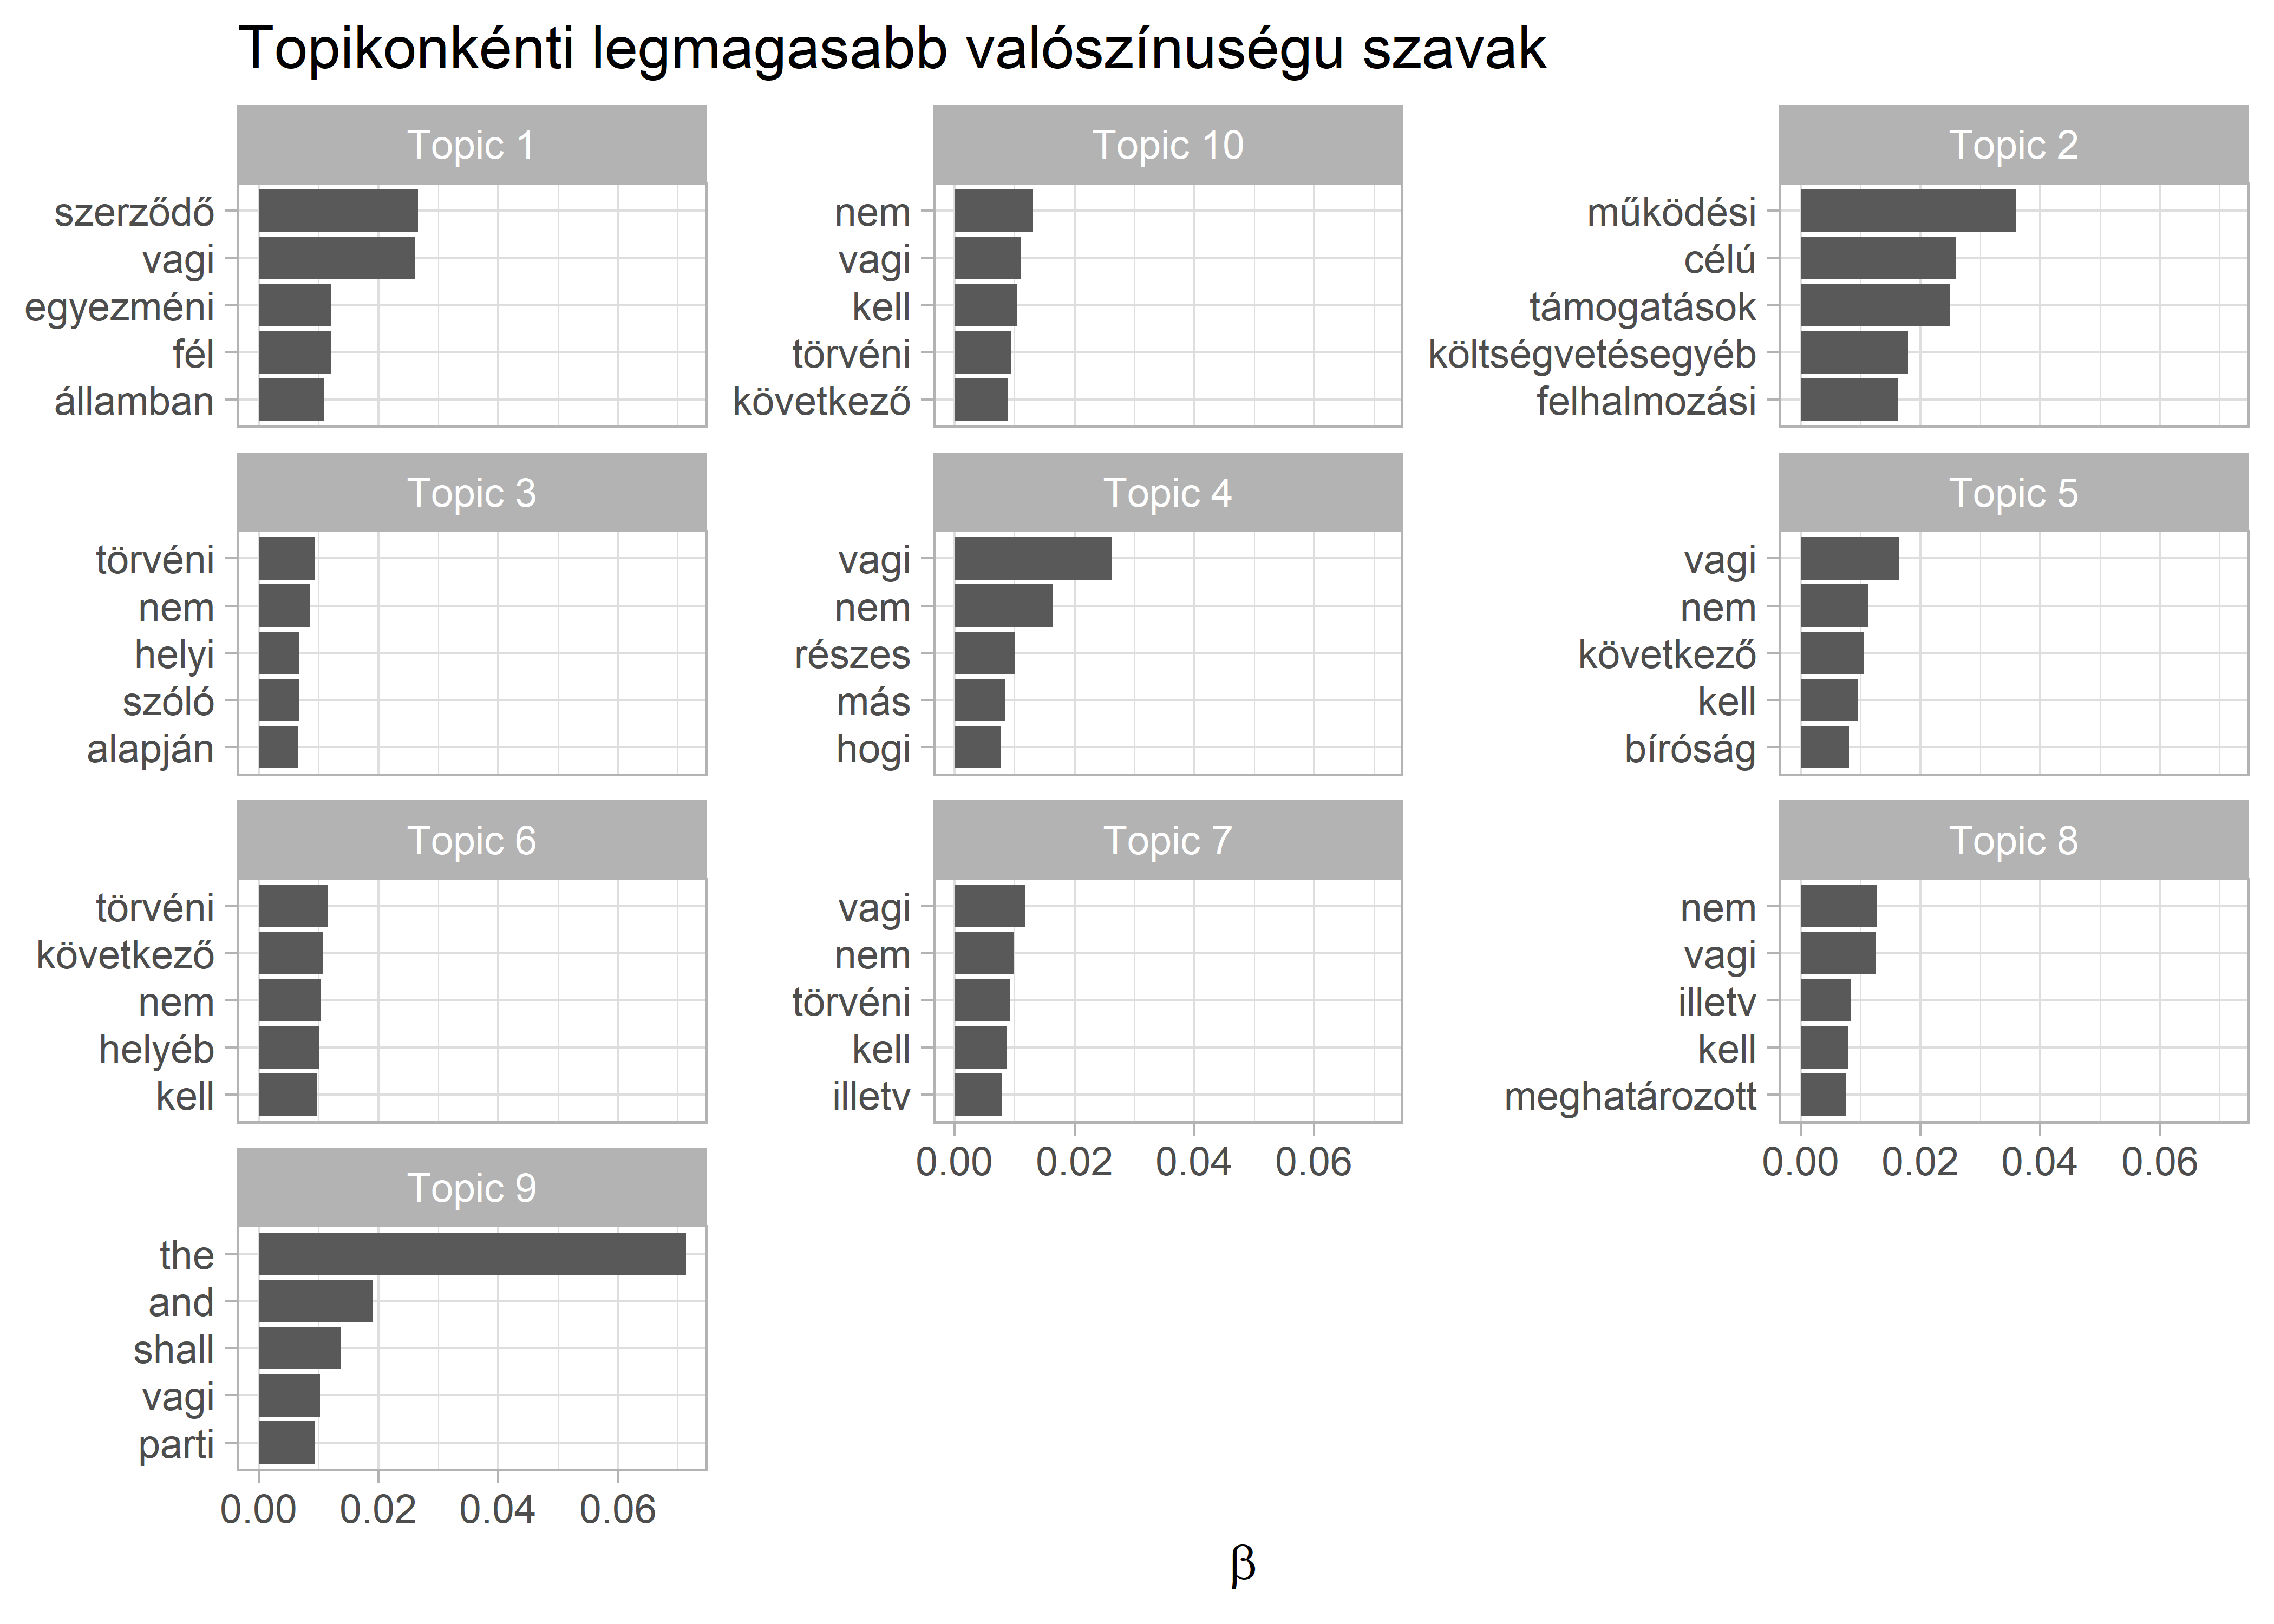
\includegraphics[width=0.9\linewidth]{_main_files/figure-latex/unnamed-chunk-101-1} \end{center}

Egy-egy topichoz tartozó meghatározó szavak annak függvényében
változhatnak hogy milyen algoritmust használunk. A
\texttt{labelTopics()} a már becsült stm modellünket alapul véve kínál 4
féle alternatív opciót. Az egyes algoritmusok részletes magyarázatáért
érdemes elolvasni a csomag részletes leírását.\footnote{Az `stm`
  csomaghoz tartozó leírás:
  \url{https://cran.r-project.org/web/packages/stm/vignettes/stmVignette.pdf}}

\begin{Shaded}
\begin{Highlighting}[]
\FunctionTok{labelTopics}\NormalTok{(stm\_fit, }\FunctionTok{c}\NormalTok{(}\DecValTok{1}\SpecialCharTok{:}\DecValTok{2}\NormalTok{))}
\CommentTok{\#\textgreater{} Topic 1 Top Words:}
\CommentTok{\#\textgreater{}       Highest Prob: szerzodo, vagi, egyezméni, fél, államban, nem, másik }
\CommentTok{\#\textgreater{}       FREX: megadóztatható, haszonhúzója, beruházóinak, segélycsapatok, adóztatást, jövedelemadók, kijelölések }
\CommentTok{\#\textgreater{}       Lift: árucikkeket, átalányösszegben, átléphetik, átszállítást, beruházóikat, célországban, cikktanulók }
\CommentTok{\#\textgreater{}       Score: szerzodo, államban, illetoségu, egyezméni, megadóztatható, adóztatható, cikka }
\CommentTok{\#\textgreater{} Topic 2 Top Words:}
\CommentTok{\#\textgreater{}       Highest Prob: muködési, célú, támogatások, költségvetésegyéb, felhalmozási, terhelo, beruházási }
\CommentTok{\#\textgreater{}       FREX: kiadásokfelújításegyéb, kiadásokintézményi, kiadásokközponti, költségvetésfelhalmozási, kiadásokkormányzati, felújításegyéb, rek }
\CommentTok{\#\textgreater{}       Lift: a+b+c, a+b+c+d, adago, adódóa, adósságállományából, adósságrendezésr, adótartozásának }
\CommentTok{\#\textgreater{}       Score: költségvetésegyéb, költségvetésszemélyi, kiadásokfelhalmozási, járulékokdolog, költségvetésintézményi, kiadásokegyéb, juttatásokmunkaadókat}
\end{Highlighting}
\end{Shaded}

A korpuszunkon belüli témák megoszlását a \texttt{plot.STM()}-el tudjuk
ábrázolni. Jól látszik hogy a Topic 2-be tartozó szavak vannak jelen a
legnagyobb arányban a dokumentumaink között.

\begin{Shaded}
\begin{Highlighting}[]
\FunctionTok{plot.STM}\NormalTok{(stm\_fit, }\StringTok{"summary"}\NormalTok{)}
\end{Highlighting}
\end{Shaded}

\begin{center}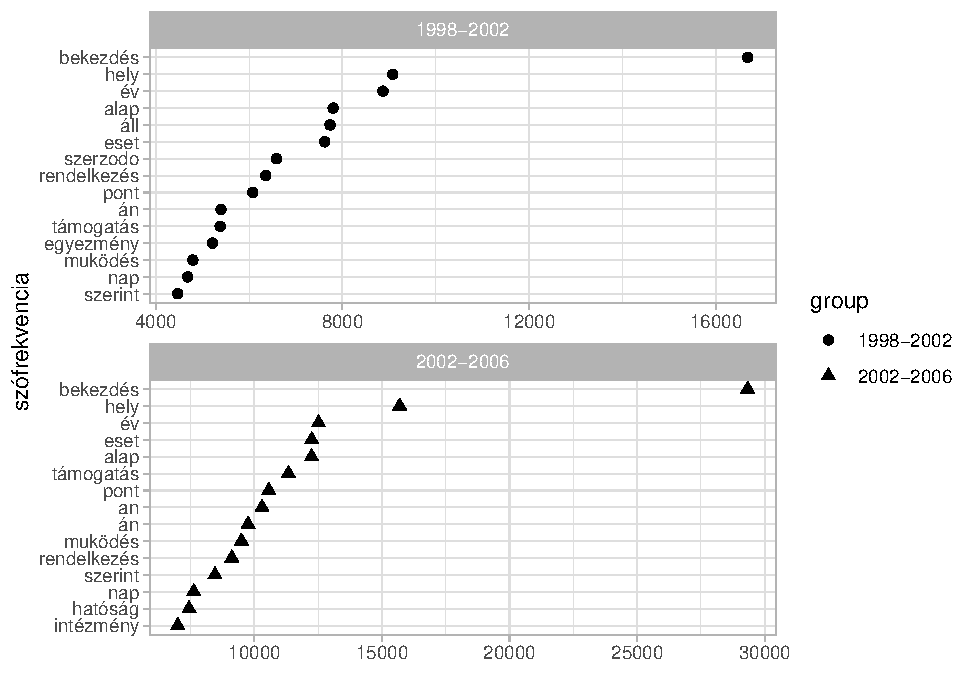
\includegraphics[width=0.9\linewidth]{_main_files/figure-latex/unnamed-chunk-103-1} \end{center}

Végezetül, a témák közötti korrelációt a \texttt{topicCorr} függvénnyel
becsülhetjük és az \texttt{igraph} csomagot betöltve a \texttt{plot()}
paranccsal tudjuk vizualizálni. Az eredmény egy hálózat lesz amit
gráfként ábrázolunk. Az élei a gráfoknak a témák közötti összefüggést
jelölik.

\begin{Shaded}
\begin{Highlighting}[]

\FunctionTok{library}\NormalTok{(igraph)}

\FunctionTok{plot}\NormalTok{(}\FunctionTok{topicCorr}\NormalTok{(stm\_fit))}
\end{Highlighting}
\end{Shaded}

\begin{center}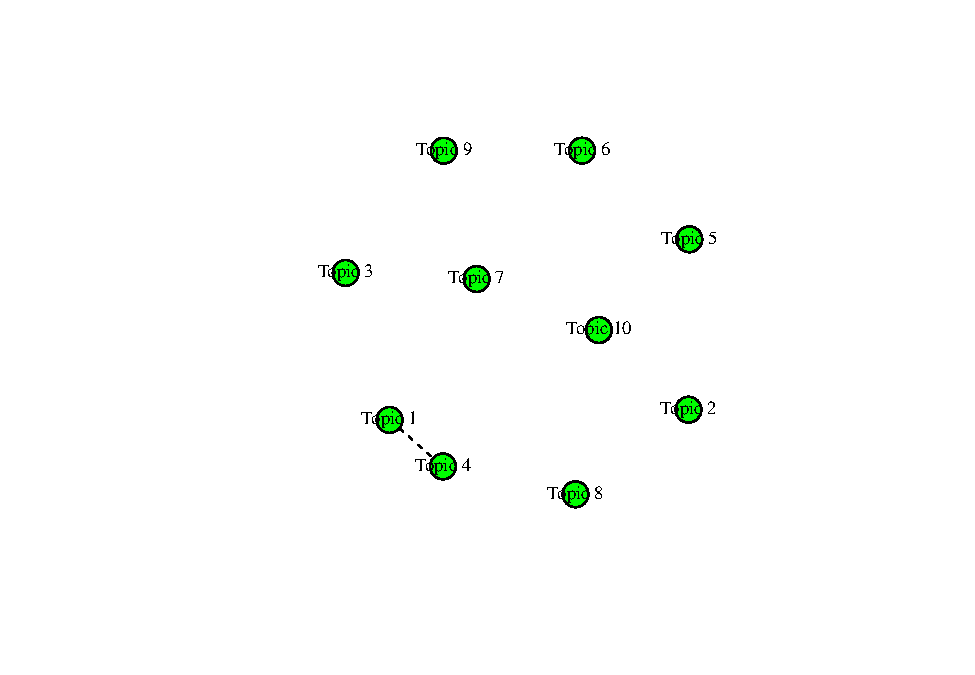
\includegraphics[width=0.9\linewidth]{_main_files/figure-latex/unnamed-chunk-104-1} \end{center}

\hypertarget{szuxf3beuxe1gyazuxe1sok}{%
\chapter{Szóbeágyazások}\label{szuxf3beuxe1gyazuxe1sok}}

kilencedik fejezet

\hypertarget{szuxf6veguxf6sszehasonluxedtuxe1s}{%
\chapter{Szövegösszehasonlítás}\label{szuxf6veguxf6sszehasonluxedtuxe1s}}

tizedik fejezet

\hypertarget{termuxe9szetes-nyelv-feldolgozuxe1s-nlp}{%
\chapter{Természetes-nyelv feldolgozás
(NLP)}\label{termuxe9szetes-nyelv-feldolgozuxe1s-nlp}}

tizenegyedik fejezet

\hypertarget{osztuxe1lyozuxe1s-uxe9s-feluxfcgyelt-tanuluxe1s}{%
\chapter{Osztályozás és felügyelt
tanulás}\label{osztuxe1lyozuxe1s-uxe9s-feluxfcgyelt-tanuluxe1s}}

tizenkeddik fejezet

\hypertarget{fuxfcggeluxe9k}{%
\chapter{Függelék}\label{fuxfcggeluxe9k}}

\hypertarget{az-r-uxe9s-az-rstudio-hasznuxe1lata}{%
\section{Az R és az RStudio
használata}\label{az-r-uxe9s-az-rstudio-hasznuxe1lata}}

Az R egy programozási nyelv, amely alkalmas statisztikai számítások
elvégzésére és ezek eredményeinek grafikus megjelenítésére. Az R
ingyenes, nyílt forráskódú szoftver, mely telepíthető mind Windows, mind
Linux, mind MacOS operációs rendszerek alatt, az alábbi oldalról:
\url{https://cran.r-project.org/} Az RStudio az R integrált fejlesztői
környezete (\emph{integrated development environment, IDE}), mely egy
olyan felhasználóbarát felületet biztosít, ami egyszerűbb és átláthatóbb
munkát tesz lehetővé. Az RStudio az alábbi oldalról tölthető le:
\url{https://rstudio.com/products/rstudio/download/}

A „point and click" szoftverekkel szemben az R használata során kódot
kell írni, ami bizonyos programozási jártasságot feltételez, de a
későbbiekben lehetővé teszi azt adott kutatási kérdéshez maximálisan
illeszkedő kódok összeállítását, melyek segítségével az elemzések mások
számára is megbízhatóan reprodukálhatóak lesznek. Ugyancsak az R
használata mellett szól, hogy komoly fejlesztői és felhasználói
közösséggel rendelkezik, így a használat során felmerülő problémákra
általában gyorsan megoldást találhatunk.

\hypertarget{az-rstudio-kezdux151feluxfclete}{%
\subsection{Az RStudio
kezdőfelülete}\label{az-rstudio-kezdux151feluxfclete}}

Az RStudio kezdőfelülete négy panelből, eszközsorból és menüsorból áll:

\begin{figure}

{\centering \includegraphics[width=0.9\linewidth]{figures/13-01_layout} 

}

\caption{RStudio felhasználói felület}\label{fig:unnamed-chunk-105}
\end{figure}

Az \textbf{\emph{(1) editor}} ablak szolgál a kód beírására, futtatására
és mentésére. A \textbf{\emph{(2) console}} ablakban jelenik meg a
lefuttatott kód és az eredmények. A jobb felső ablak \textbf{\emph{(3)
environment}} fülén láthatóak a memóriában tárolt adatállományok,
változók és felhasználói függvények. A \textbf{\emph{history}} fül
mutatja a korábban lefuttatott utasításokat. A jobb alsó ablak
\textbf{\emph{(4) files}} fülén az aktuális munkakönyvtárban levő
mappákat és fájlok találjuk, míg a \textbf{\emph{plot}} fülön az
elemzéseink során elkészített ábrák jelennek meg. A
\textbf{\emph{packages}} fülön frissíthetjük a meglévő r csomagokat és
telepíthetünk újakat. A \textbf{\emph{help}} fülön a különböző
függvények, parancsok leírását, és használatát találjuk meg. A
\texttt{Tools\ -\textgreater{}\ Global\ Options} menüpont végezhetjük el
az RStudio testreszabását. Így például beállíthatjuk az ablaktér
elrendezését (\emph{Pane layout}), vagy a színvilágot
(\emph{Appearance}), illetve azt hogy a kódok ne fussanak ki az ablakból
(\texttt{Code\ -\textgreater{}\ Editing\ -\textgreater{}\ Soft\ wrap\ R\ source\ files})

\hypertarget{projektmunka}{%
\subsection{Projekt alapú munka}\label{projektmunka}}

Bár nem kötelező, de javasolt, hogy az RStudio-ban projekt alapon
dolgozzunk, mivel így az összes -- az adott projekttel kapcsolatos fájlt
-- egy mappában tárolhatjuk. Új projekt beállítását a
\texttt{File-\textgreater{}New\ Project} menüben tehetjük meg, ahol a
saját gépünk egy könyvtárát kell kiválasztani, ahová az R scripteket, az
adat- és előzményfájlokat menti. Ezenkívül a
\texttt{Tools-\textgreater{}Global\ Options-\textgreater{}General}
menüpont alatt le kell tiltani a \emph{„Restore most recently opened
project at startup''} és a \emph{„Restore .RData ino workspace at
startup''} beállítást, valamint \emph{„Save workspace to .RData on
exit''} értékre be kell állítani a \emph{„Never''} értéket.

\begin{figure}

{\centering \includegraphics[width=0.9\linewidth]{figures/13-02_project_options} 

}

\caption{RStudio projekt beállítások}\label{fig:unnamed-chunk-106}
\end{figure}

A szükséges beállítások után a
\texttt{File\ -\textgreater{}\ New\ Project} menüben hozhatjuk létre a
projektet. Itt arra is lehetőségünk van, hogy kiválasszuk, hogy a
projektünket egy teljesen új könyvtárba, vagy egy meglévőbe kívánjuk
menteni, esetleg egy meglévő projekt új verzióját szeretnénk létrehozni.
Ha sikeresen létrehoztuk a projektet, az RStudio jobb felső sarkában
látnunk kell annak nevét.

\hypertarget{scriptek-szerkesztuxe9se-fuxfcggvuxe9nyek-hasznuxe1lata}{%
\subsection{Scriptek szerkesztése, függvények
használata}\label{scriptek-szerkesztuxe9se-fuxfcggvuxe9nyek-hasznuxe1lata}}

Új script a
\texttt{File\ -\textgreater{}\ New\ -\textgreater{}\ File\ -\textgreater{}\ R}
Script menüpontban hozható létre, mentésére a File-\textgreater Save
menüpontban egy korábbi script megnyitására
\texttt{File\ -\textgreater{}\ Open} menüpontban van lehetőségünk.
Script bármilyen szövegszerkesztővel írható és beilleszthető az editor
ablakba. A scripteket érdemes magyarázatokkal (kommentekkel) ellátni,
hogy a későbbiekben pontosan követhető legyen, hogy melyik parancs
segítségével pontosan milyen lépéseket hajtottunk végre. A
magyarázatokat vagy más néven kommenteket kettőskereszt (\texttt{\#})
karakterrel vezetjük be. A scriptbeli utasítások az azokat tartalmazó
sorokra állva vagy több sort kijelölve a Run feliratra kattintva vagy a
\texttt{Ctrl+Enter} billentyűparanccsal futtathatók le. A lefuttatott
parancsok és azok eredményei ezután a bal alsó sarokban lévő console
ablakban jelennek meg és ugyanitt kapunk hibaüzenetet is, ha valamilyen
hibát vétettünk a scriptben.

A munkafolyamat során létrehozott állományok (ábrák, fájlok) ebbe az ún.
munkakönyvtárba (\emph{working directory}) mentődnek. Az aktuális
munkakönyvtár neve, elérési útja a \texttt{getwd()} utasítással
jeleníthető meg. A könyvtárban található állományok listázására a
\texttt{list.files()} utasítással van lehetőségünk. Ha a korábbiaktól
eltérő munkakönyvtárat akarunk megadni, azt a \texttt{setwd()}
függvénnyel tehetjük meg, ahol a ()-ben az adott mappa elérési útját
kell megadnunk. Az elérési útban a meghajtó azonosítóját, majd a mappák,
almappák nevét vagy egy normál irányú perjel (\texttt{/}), vagy két
fordított perjel (\texttt{\textbackslash{}\textbackslash{}}) választja
el, mivel az elérési út karakterlánc, ezért azt idézőjelek vagy
aposztrófok közé kell tennünk. Az aktuális munkakönyvtárba beléphetünk a
jobb alsó ablak file lapján a
\texttt{„More\ -\textgreater{}\ Go\ To\ Working\ Directory”}
segítségével. Ugyanitt a \texttt{„Set\ Working\ Directory”}-val
munkakönyvtárnak állíthatjuk be az a mappát, amelyben épp benne vagyunk.

\begin{figure}

{\centering \includegraphics[width=0.9\linewidth]{figures/13-03_working_directory} 

}

\caption{Working directory beállítások}\label{fig:unnamed-chunk-107}
\end{figure}

A munkafolyamat befejezésére a \texttt{q()} vagy \texttt{quit()}
függvényel van lehetőségünk. A munkafolyamat során különböző
objektumokat hozunk létre, melyek az RStudio jobb felső ablakának
environment fülén jelennek meg, a mentett objektumokat a fent látható
seprű ikonra kattintva törölhetjük a memóriából. Az environment ablakra
érdemes úgy gondolni hogy ott jelennek meg a memóriában tárolt értékek.
Az R-ben objektumokkal dolgozunk, amik a teljesség igénye nélkül
lehetnek egyszerű szám vektortok, vagy akár komplex listák, illetve
függvények, ábrák.

Az RStudio jobb alsó ablakának plots fülén láthatjuk azon parancsok
eredményét, melyek kimenete valamilyen ábra. A packages fülnél a már
telepített és a letölthető kiegészítő csomagokat jeleníthetjük meg. A
help fülön a korábban említettek szerint a súgó érhető el. Az
RStudio-ban használható billentyűparancsok teljes listáját Alt+Shift+K
billentyűkombinációval tekinthetjük meg. Néhány gyakrabban használt,
hasznos billentyűparancs:

\begin{itemize}
\tightlist
\item
  \texttt{Ctrl+Enter}: futtassa a kódot az aktuális sorban
\item
  \texttt{Ctrl+Alt+B}: futtassa a kódot az elejétől az aktuális sorig
\item
  \texttt{Ctrl+Alt+E}: futtassa a kódot az aktuális sortól a forrásfájl
  végéig
\item
  \texttt{Ctrl+D}: törölje az aktuális sort
\end{itemize}

Az R-ben beépített \textbf{függvények (function)} állnak
rendelkezésünkre a számítások végrehajtására, emellett több
\textbf{csomag (package)} is letölthető, amelyek különböző függvényeket
tartalmaznak. A függvények a következőképpen épülnek fel:
\texttt{függvénynév(paraméter)}. Például tartalom képernyőre való
kiíratását a \texttt{print()} függvénnyel tehetjük, amelynek gömbölyű
zárójelekkel határolt részébe írhatjuk a megjelenítendő szöveget. A
\texttt{citation()} függvénnyel lekérdezhetjük az egyes beépített
csomagokra való hivatkozást is: a \texttt{citation(quanteda)} függvény a
quanteda csomag hivatkozását adja meg. Az R súgórendszere a
\texttt{help.start()} utasítással indítható el. Egy adott függvényre
vonatkozó súgórészlet a függvények neve elé kérdőjel írásával, vagy a
\texttt{help()} argumentumába a kérdéses függvény nevének beírásával
jeleníthető meg (pl.: \texttt{help(sum)}).

\hypertarget{packages}{%
\subsection{R csomagok}\label{packages}}

Az R-ben telepíthetők kiegészítő csomagok (packages), amelyek
alapértelmezetten el nem érhető algoritmusokat, függvényeket
tartalmaznak. A csomagok saját dokumentációval rendelkeznek, amelyeket
fel kell tüntetni a használatukkal készült publikációink
hivatkozáslistájában. A csomagok telepítésre több lehetőségünk is van:
használhatjuk a menüsor
\texttt{Tools\ -\textgreater{}\ Install\ Packages} menüpontját, vagy a
jobb alsó ablak \emph{Packages} fül Install menüpontját, illetve az
editor ablakban az \texttt{install.packages()} parancsot futtatva, ahol
a ()-be a telepíteni kívánt csomag nevét kell beírnunk (pl.:
\texttt{install.packages(dplyr)}).

\begin{figure}

{\centering \includegraphics[width=0.9\linewidth]{figures/13-04_packages} 

}

\caption{Packages fül}\label{fig:unnamed-chunk-108}
\end{figure}

\hypertarget{objektumok-tuxe1roluxe1sa-uxe9rtuxe9kaduxe1s}{%
\subsection{Objektumok tárolása,
értékadás}\label{objektumok-tuxe1roluxe1sa-uxe9rtuxe9kaduxe1s}}

Az objektumok lehetnek például \emph{vektorok}, \emph{mátrixok}
(matrix), \emph{tömbök} (array), \emph{adat táblák} (data frame).
Értékadás nélkül az R csak megjeleníti a műveletek eredményét, de nem
tárolja el azokat. Az eredmények eltárolásához azokat egy objektumba
kell elmentenünk. Ehhez meg kell adnunk az objektum nevét majd az
\texttt{\textless{}-} után adjuk meg annak értékét:
\texttt{a\ \textless{}-\ 12\ +\ 3}.Futtatás után az environments fülön
megjelenik az a objektum, melynek értéke \texttt{15}. Az objektumok
elnevezésénél figyelnünk kell arra, hogy az R különbséget tesz a kis és
nagybetűk között, valamint, hogy az ugyanolyan nevű objektumokat kérdés
nélkül felülírja és ezt a felülírást nem lehet visszavonni.

\hypertarget{vektorok}{%
\subsection{Vektorok}\label{vektorok}}

Az R-ben kétféle típusú vektort különböztetünk meg:

\begin{itemize}
\tightlist
\item
  egyedüli vektor (atomic vector)
\item
  lista (list)
\end{itemize}

Az egyedüli vektornak hat típusa van, \textbf{logikai} (logical),
\textbf{egész szám} (integer), \textbf{természetes szám} (double),
\textbf{karakter} (character), \textbf{komplex szám} (complex) és
\textbf{nyers adat} (raw). A leggyakrabban valamilyen numerikus, logikai
vagy karakter vektorral használjuk. Az egyedüli vektorok onnan kapták a
nevüket hogy csak egy féle adattípust tudnak tárolni. A listák ezzel
szemben gyakorlatilag bármit tudnak tárolni, akár több listát is
egybeágyazhatunk.

A vektorok és listák azok az építőelemek amikből felépülnek az R
objektumaink. Több érték vagy azonos típusú objektum összefűzését a
\texttt{c()} függvénnyel végezhetjük el. A lenti példában három
különböző objektumot kreálunk, egy numerikusat, egy karaktert és egy
logikait. A karakter vektorban az elemeket időzőjellel és vesszővel
szeparáljuk. A logikai vektor csak \texttt{TRUE}, illetve \texttt{FALSE}
értékeket tartalmazhat.

\begin{Shaded}
\begin{Highlighting}[]
\NormalTok{numerikus }\OtherTok{\textless{}{-}} \FunctionTok{c}\NormalTok{(}\DecValTok{1}\NormalTok{, }\DecValTok{2}\NormalTok{, }\DecValTok{3}\NormalTok{, }\DecValTok{4}\NormalTok{, }\DecValTok{5}\NormalTok{)}

\NormalTok{karakter }\OtherTok{\textless{}{-}} \FunctionTok{c}\NormalTok{(}\StringTok{"kutya"}\NormalTok{, }\StringTok{"macska"}\NormalTok{, }\StringTok{"ló"}\NormalTok{)}

\NormalTok{logikai }\OtherTok{\textless{}{-}} \FunctionTok{c}\NormalTok{(}\ConstantTok{TRUE}\NormalTok{, }\ConstantTok{TRUE}\NormalTok{, }\ConstantTok{FALSE}\NormalTok{)}
\end{Highlighting}
\end{Shaded}

A létrehozott vektorokkal különböző műveleteket végezhetünk el, például
összeadhatjuk numerikus vektorainkat. Ebben az esetben az első vektor
első eleme a második vektor első eleméhez adódik.

\begin{Shaded}
\begin{Highlighting}[]
\FunctionTok{c}\NormalTok{(}\DecValTok{1}\SpecialCharTok{:}\DecValTok{4}\NormalTok{) }\SpecialCharTok{+} \FunctionTok{c}\NormalTok{(}\DecValTok{10}\NormalTok{, }\DecValTok{20}\NormalTok{, }\DecValTok{30}\NormalTok{, }\DecValTok{40}\NormalTok{)}
\CommentTok{\#\textgreater{} [1] 11 22 33 44}
\end{Highlighting}
\end{Shaded}

A karaktervektorokat összefűzhetjük egymással. Itt egy új objektumot is
létrehoztunk, a jobb felső ablakban, az environment fülön láthatjuk,
hogy a létrejött karakter\_kombinalt objektum egy négy elemű
(hosszúságú) karaktervektor (\texttt{chr\ {[}1:4{]}}), melynek elemei a
\texttt{"kutya","macska","ló","nyúl"}. Az objektumként tárolt vektorok
tartalmát a lefuttatva írathatjuk ki a console ablakba. Habár van
\texttt{print()} függvény az R-ben, azt ilyenkor nem szükséges
használni.

\begin{Shaded}
\begin{Highlighting}[]
\NormalTok{karakter1 }\OtherTok{\textless{}{-}} \FunctionTok{c}\NormalTok{(}\StringTok{"kutya"}\NormalTok{, }\StringTok{"macska"}\NormalTok{, }\StringTok{"ló"}\NormalTok{)}
\NormalTok{karakter2 }\OtherTok{\textless{}{-}} \FunctionTok{c}\NormalTok{(}\StringTok{"nyúl"}\NormalTok{)}

\NormalTok{karakter\_kombinalt }\OtherTok{\textless{}{-}} \FunctionTok{c}\NormalTok{(karakter1, karakter2)}

\NormalTok{karakter\_kombinalt}
\CommentTok{\#\textgreater{} [1] "kutya"  "macska" "ló"     "nyúl"}
\end{Highlighting}
\end{Shaded}

Ha egy vektorról szeretnénk megtudni, hogy milyen típusú azt a
\texttt{typeof()} vagy a \texttt{class()} paranccsal tehetjük meg, ahol
()-ben az adott objektumként tárolt vektor nevét kell megadnunk:
\texttt{typeof(karakter1)}. A vektor hosszúságát (benne tárolt elemek
száma vektorok esetén) a \texttt{lenght()} függvénnyel tudhatjuk meg.

\begin{Shaded}
\begin{Highlighting}[]
\FunctionTok{typeof}\NormalTok{(karakter1)}
\CommentTok{\#\textgreater{} [1] "character"}

\FunctionTok{length}\NormalTok{(karakter1)}
\CommentTok{\#\textgreater{} [1] 3}
\end{Highlighting}
\end{Shaded}

\hypertarget{faktorok}{%
\subsection{Faktorok}\label{faktorok}}

A faktorok a kategórikus adatok tárolására szolgálnak. Faktor típusú
változó a \texttt{factor()} függvénnyel hozható létre. A faktor
szintjeit (igen, semleges, nem), a \texttt{levels()} függvénnyel
kaphatjuk meg míg az adatok címkéit (tehát a kapott válaszok száma), a
\texttt{labels()} paranccsal érhetjük el.

\begin{Shaded}
\begin{Highlighting}[]
\NormalTok{survey\_response }\OtherTok{\textless{}{-}} \FunctionTok{factor}\NormalTok{(}\FunctionTok{c}\NormalTok{(}\StringTok{"igen"}\NormalTok{, }\StringTok{"semleges"}\NormalTok{, }\StringTok{"nem"}\NormalTok{, }\StringTok{"semleges"}\NormalTok{, }\StringTok{"nem"}\NormalTok{, }\StringTok{"nem"}\NormalTok{, }\StringTok{"igen"}\NormalTok{), }\AttributeTok{ordered =} \ConstantTok{TRUE}\NormalTok{)}


\FunctionTok{levels}\NormalTok{(survey\_response)}
\CommentTok{\#\textgreater{} [1] "igen"     "nem"      "semleges"}

\FunctionTok{labels}\NormalTok{(survey\_response)}
\CommentTok{\#\textgreater{} [1] "1" "2" "3" "4" "5" "6" "7"}
\end{Highlighting}
\end{Shaded}

\hypertarget{data-frame}{%
\subsection{Data frame}\label{data-frame}}

Az adat táblák (data frame) a statisztikai és adatelemzési folyamatok
egyik leggyakrabban használt adattárolási formája. Amikor lehetséges
akkor a `hosszú' formátumban használjuk (az R közösség a `tidy' jelzővel
illeti), aholtéglalap alakú adatszerkezetek, ahol minden sor egy
megfigyelés és minden oszlop egy változó {[}TIDY CITATION{]}. Egy data
frame többféle típusú adatot tartalmazhat. A data frame-k különféle
oszlopokból állhatnak, amelyek különféle típusú adatokat
tartalmazhatnak, de egy oszlop csak egy típusú adatból állhat. A lent
bemutatott data frame 7 megfigyelést és 4 féle változót tartalmaz (id,
country, pop, continent).

\begin{verbatim}
#>   id      orszag nepesseg     kontinens
#> 1  1    Thailand     68.7          Asia
#> 2  2      Norway      5.2        Europe
#> 3  3 North Korea     24.0          Asia
#> 4  4      Canada     47.8 North America
#> 5  5    Slovenia      2.0        Europe
#> 6  6      France     63.6        Europe
#> 7  7   Venezuela     31.6 South America
\end{verbatim}

A data frame-be rendezett adatokhoz különböző módon férhetünk hozzá,
például a data frame nevének majd {[}{]}-ben a kívánt sor megadásával,
kiírathatjuk a console ablakba annak tetszőleges sorát ás oszlopát:
\texttt{orszag\_adatok{[}1,\ 1{]}}. Az R több különböző módot kínál a
data frame sorainak és oszlopainak eléréséhez. A \texttt{{[}} általános
használata: \texttt{data\_frame{[}sor,\ oszlop{]}}. Egy másik megoldás a
\texttt{\$} haszálata: \texttt{data\_frame\$oszlop}.

\begin{Shaded}
\begin{Highlighting}[]
\NormalTok{orszag\_adatok[}\DecValTok{1}\NormalTok{, }\DecValTok{4}\NormalTok{]}
\CommentTok{\#\textgreater{} [1] Asia}
\CommentTok{\#\textgreater{} Levels: Asia Europe North America South America}

\NormalTok{orszag\_adatok}\SpecialCharTok{$}\NormalTok{orszag}
\CommentTok{\#\textgreater{} [1] "Thailand"    "Norway"      "North Korea" "Canada"      "Slovenia"   }
\CommentTok{\#\textgreater{} [6] "France"      "Venezuela"}
\end{Highlighting}
\end{Shaded}

\hypertarget{vizualizuxe1ciuxf3}{%
\section{Vizualizáció}\label{vizualizuxe1ciuxf3}}

\begin{Shaded}
\begin{Highlighting}[]
\FunctionTok{library}\NormalTok{(ggplot2)}
\FunctionTok{library}\NormalTok{(gapminder)}
\end{Highlighting}
\end{Shaded}

Az elemzéseinkhez használt data frame adatainak alapján a
\texttt{ggplot2} csomag segítségével lehetőségünk van különböző
vizualizációk készítésére is.

A \texttt{ggplot2} használata során különböző témákat alkalmazhatunk,
melyek részletes leírása megtalálható:
\url{https://ggplot2.tidyverse.org/reference/ggtheme.html}

Abban az esetben, ha nem választunk témát, a \texttt{ggplot2} a
következő ábrán is látható alaptémát használja. Ha például a szürke
helyett fehér hátteret szeretnénk, alkalmazhatjuk a
\texttt{theme\_minmal()}parancsot. Szintén gyakran alkalmazott ábra alap
a \texttt{thema\_bw()}, ami az előzőtől az ábra keretezésében
különbözik. Ha fehér alapon, de a beosztások vonalait feketén szeretnénk
megjeleníteni, alkalmazhatjuk a \texttt{theme\_linedraw()} függvényt, a
\texttt{theme\_void()} segítségével pedig egy fehér alapon,
beosztásoktól mentes alapot kapunk, a \texttt{theme\_dark()} pedig sötét
hátteret eredményez. A \texttt{theme\_classic()} segítségével az x és y
tengelyt jeleníthetjük meg fehér alapon.

Egy ábra készítésének alapja mindig a használni kívánt adatkészlet
beolvasása, illetve az ábrázolni kiíván változtót vagy változók
megadása.

Ezt követi a megfelelő alakzat kiválasztása, attól függően például, hogy
eloszlást, változást, adatok közötti kapcsolatot, vagy elétéseket
akarunk ábrázolni. A \texttt{geom} az a geometriai objektum, a mit a
diagram az adatok megjelenítésére használ. A\texttt{gglpot2} több mint
40 féle alakzat alkalmazására ad lehetőséget, ezek közül néhány
gyakoribbat mutatunk be az alábbiakban. Az alakzatokról részletes
leírása található például az alábbi linken:
\url{https://r4ds.had.co.nz/data-visualisation.html}

A következőkben a már korábban is használt \texttt{gapminder} adatok
segítségével, személetetjük az adatok vizualizálásának alapjait. Először
egyszerű alapbeállítások mellett egy histogram típusú vizualizációt
készítünk.

\begin{Shaded}
\begin{Highlighting}[]
\FunctionTok{ggplot}\NormalTok{(}
  \AttributeTok{data =}\NormalTok{ gapminder,}
  \AttributeTok{mapping =} \FunctionTok{aes}\NormalTok{(}\AttributeTok{x =}\NormalTok{ gdpPercap)}
\NormalTok{) }\SpecialCharTok{+}
  \FunctionTok{geom\_histogram}\NormalTok{()}
\end{Highlighting}
\end{Shaded}

\begin{center}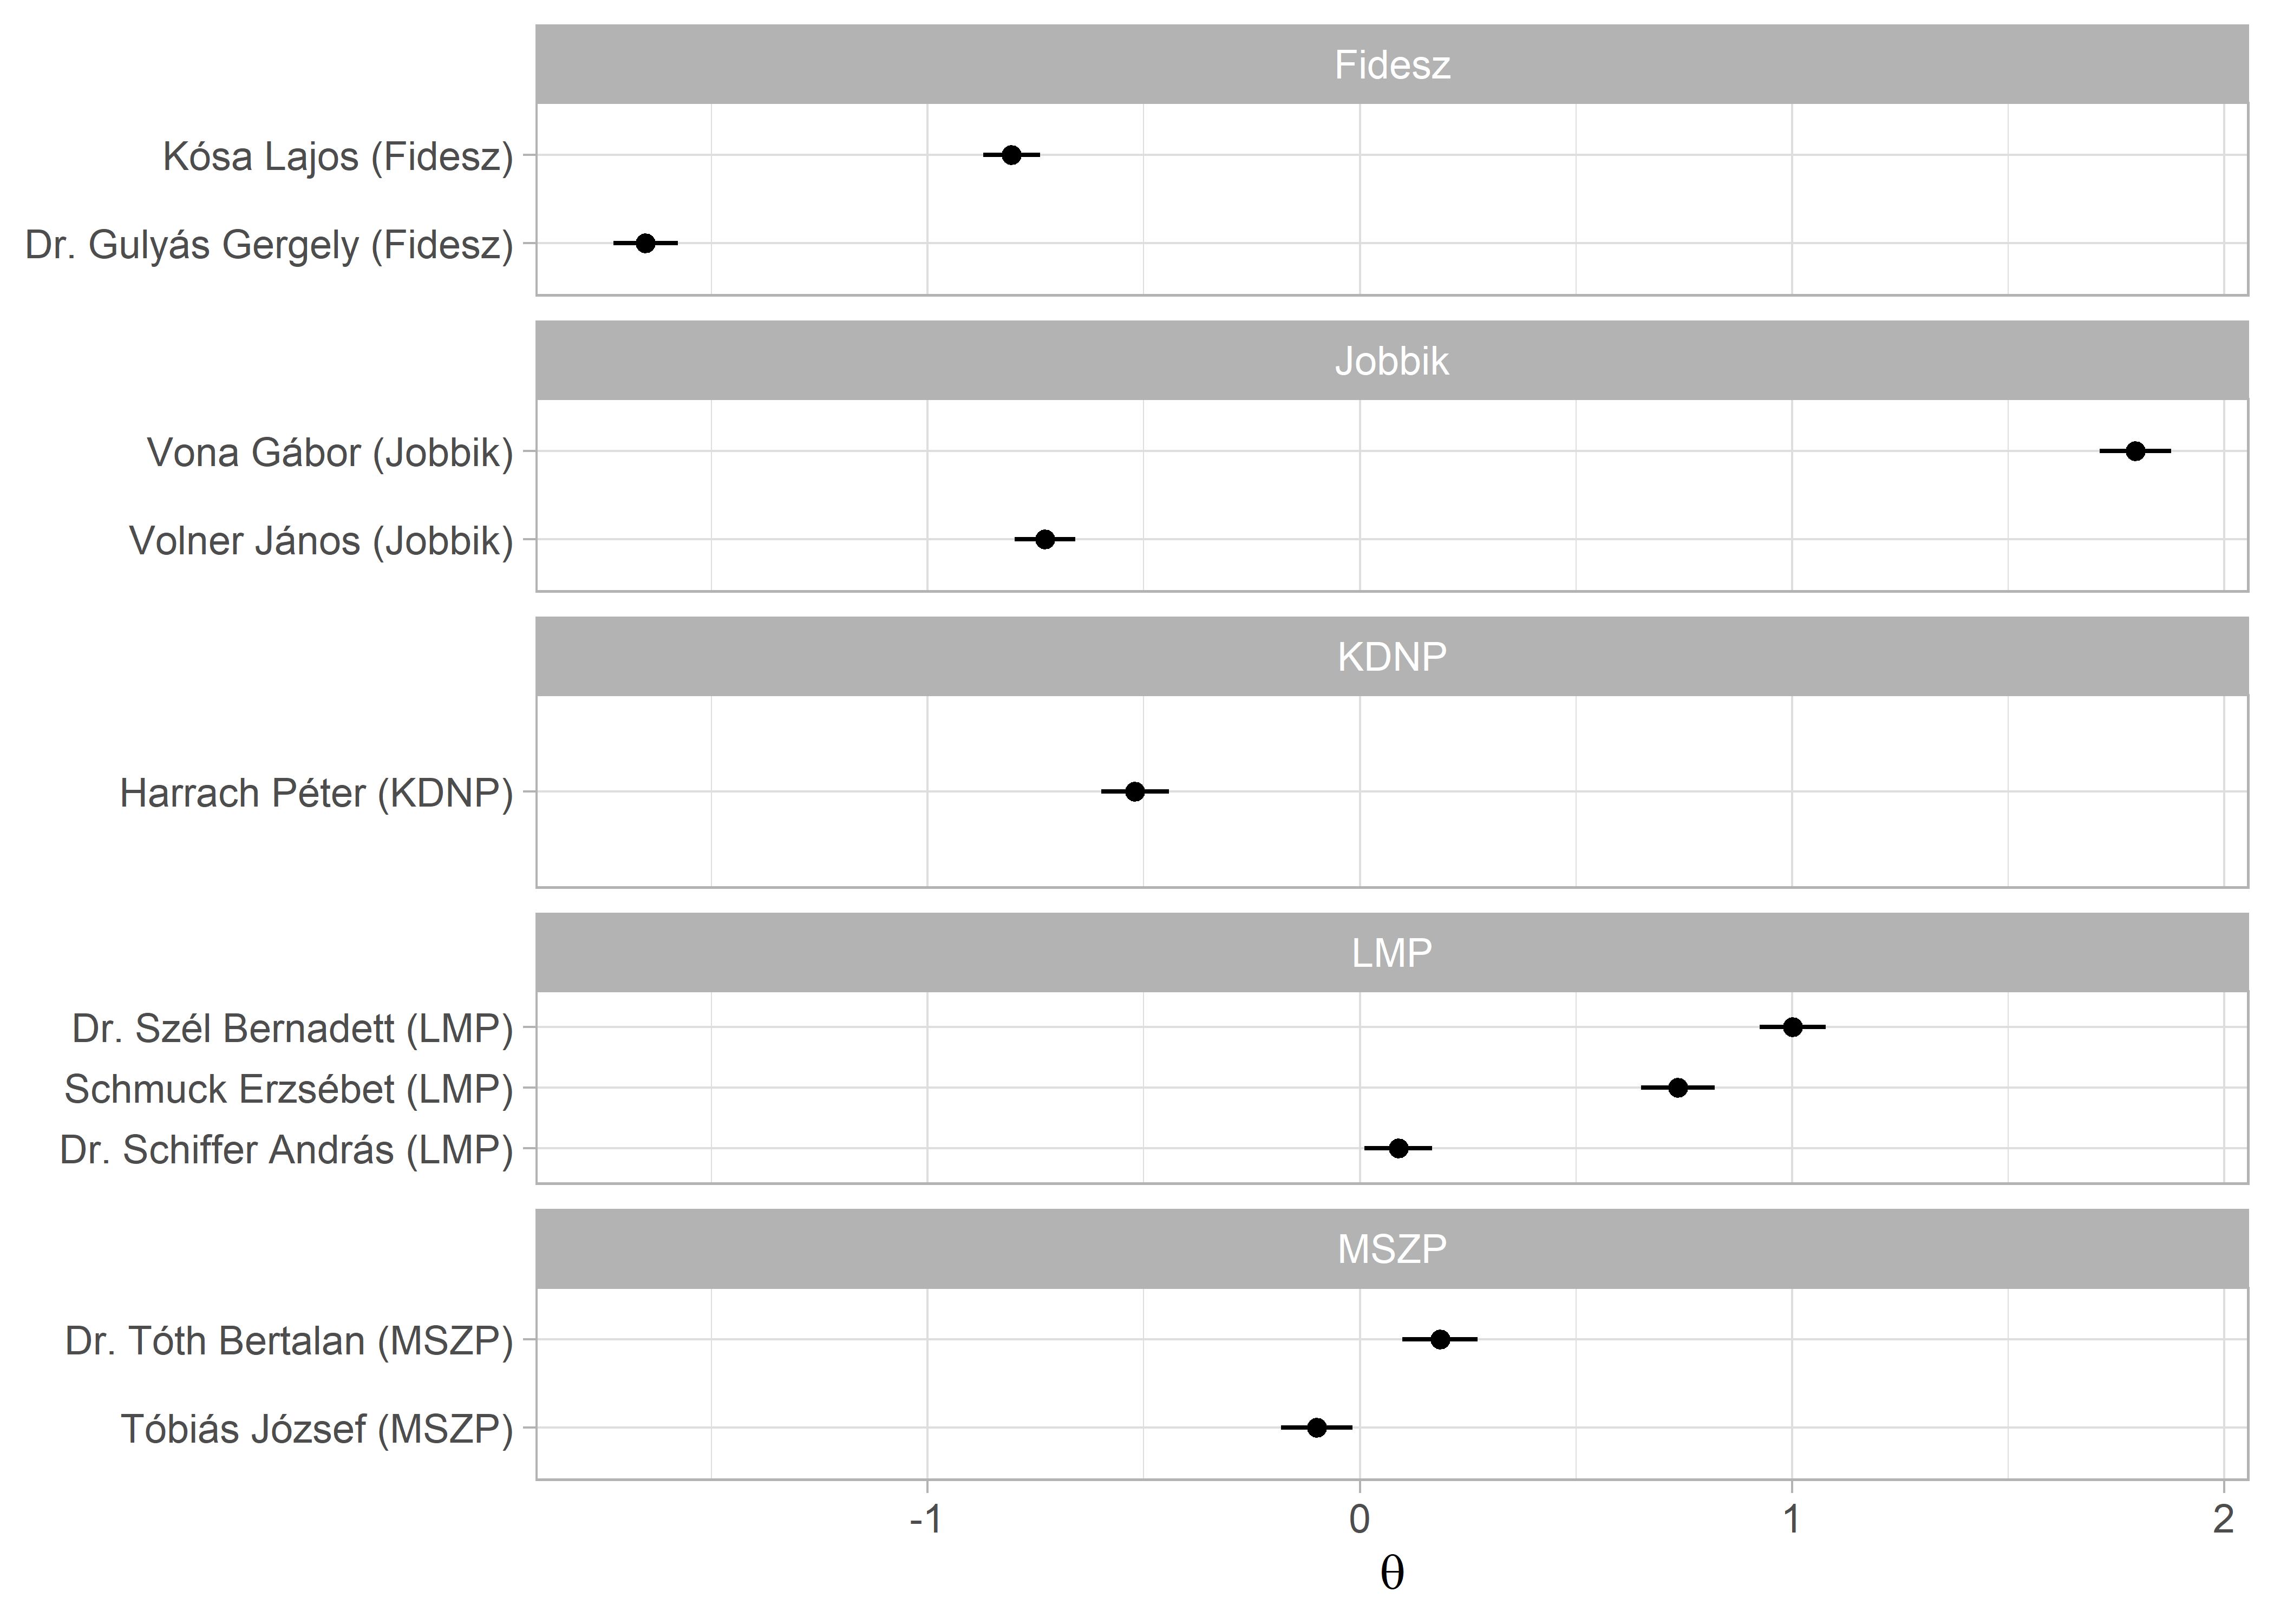
\includegraphics[width=0.9\linewidth]{_main_files/figure-latex/unnamed-chunk-118-1} \end{center}

Lehetőségünk van arra, hogy az alakzat színét megváltoztatássuk. A
használható színek és színkódok megtalálhatóak a \texttt{ggplot2}
leírásában: \url{https://ggplot2-book.org/scale-colour.html}

\begin{Shaded}
\begin{Highlighting}[]
\FunctionTok{ggplot}\NormalTok{(}
  \AttributeTok{data =}\NormalTok{ gapminder,}
  \AttributeTok{mapping =} \FunctionTok{aes}\NormalTok{(}\AttributeTok{x =}\NormalTok{ gdpPercap)}
\NormalTok{) }\SpecialCharTok{+}
  \FunctionTok{geom\_histogram}\NormalTok{(}\AttributeTok{fill =} \StringTok{"yellow"}\NormalTok{, }\AttributeTok{colour =} \StringTok{"green"}\NormalTok{)}
\end{Highlighting}
\end{Shaded}

\begin{center}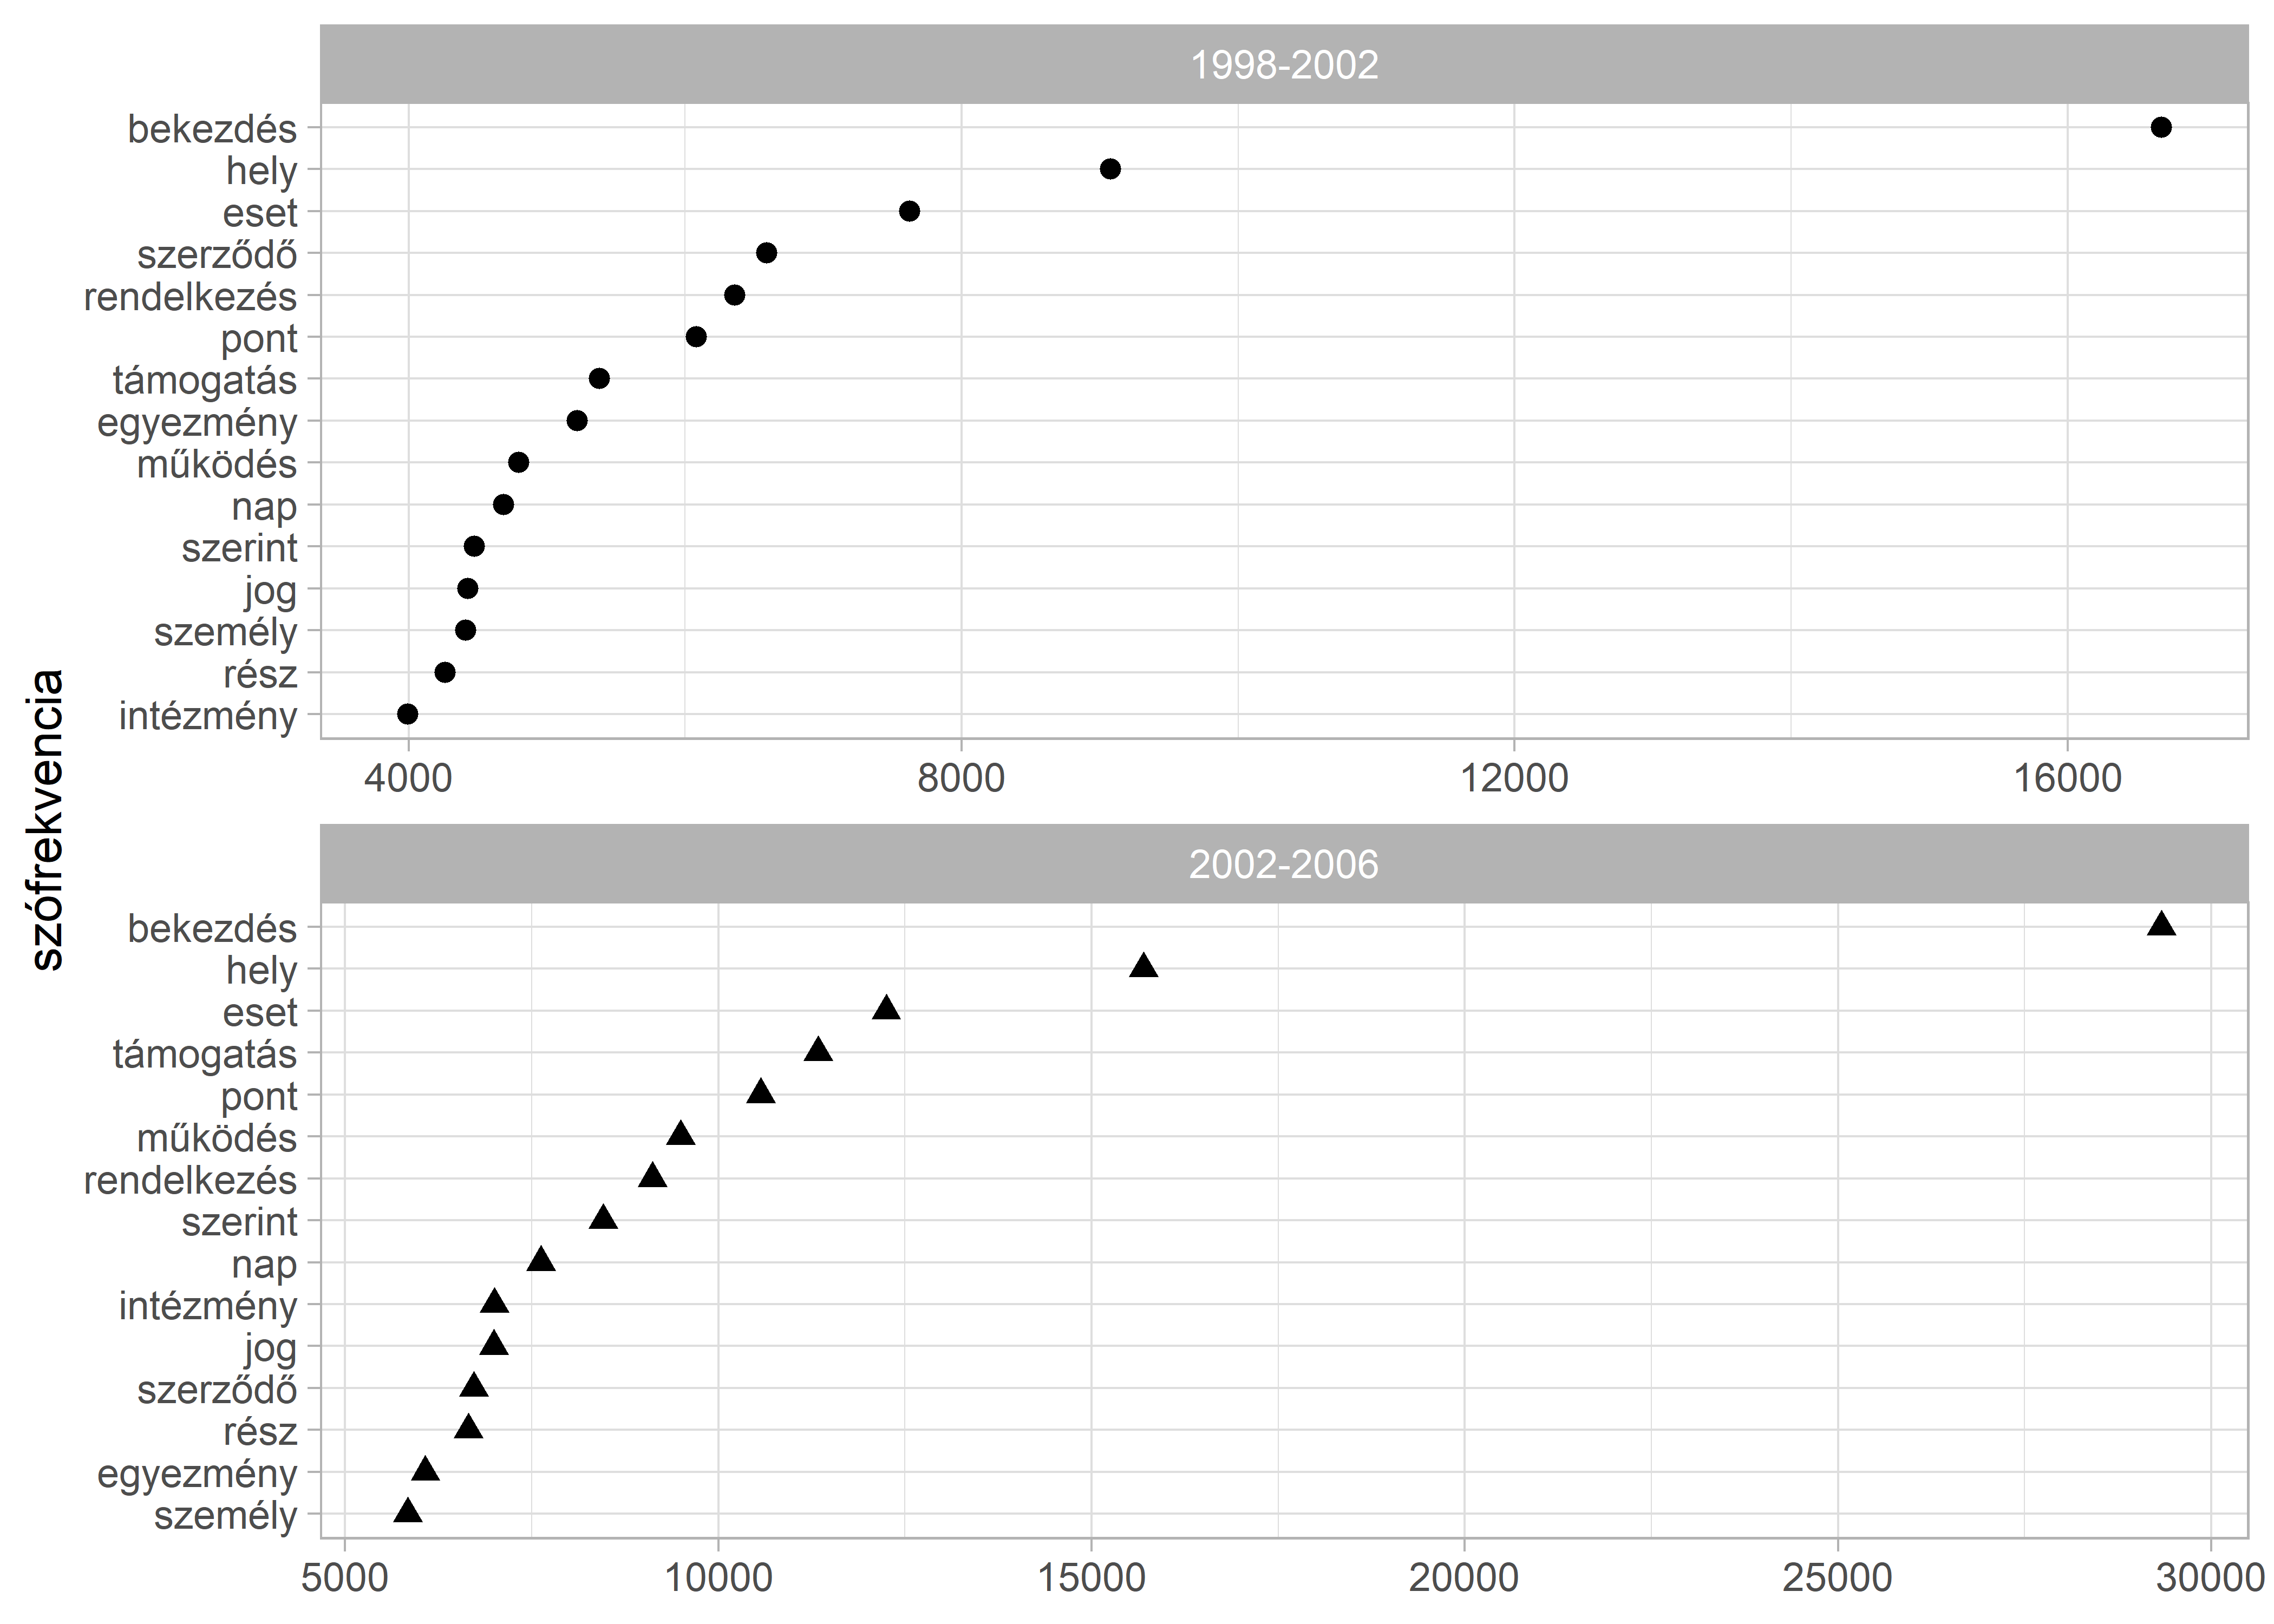
\includegraphics[width=0.9\linewidth]{_main_files/figure-latex/unnamed-chunk-119-1} \end{center}

Meghatározhatjuk külön-külön a histogram x és y tengelyén ábrázolni
kívánt adatokat és választhatjuk azok pontszerű ábrázolását is.

\begin{Shaded}
\begin{Highlighting}[]
\FunctionTok{ggplot}\NormalTok{(}
  \AttributeTok{data =}\NormalTok{ gapminder,}
  \AttributeTok{mapping =} \FunctionTok{aes}\NormalTok{(}
    \AttributeTok{x =}\NormalTok{ gdpPercap,}
    \AttributeTok{y =}\NormalTok{ lifeExp}
\NormalTok{  )}
\NormalTok{) }\SpecialCharTok{+}
  \FunctionTok{geom\_point}\NormalTok{()}
\end{Highlighting}
\end{Shaded}

\begin{center}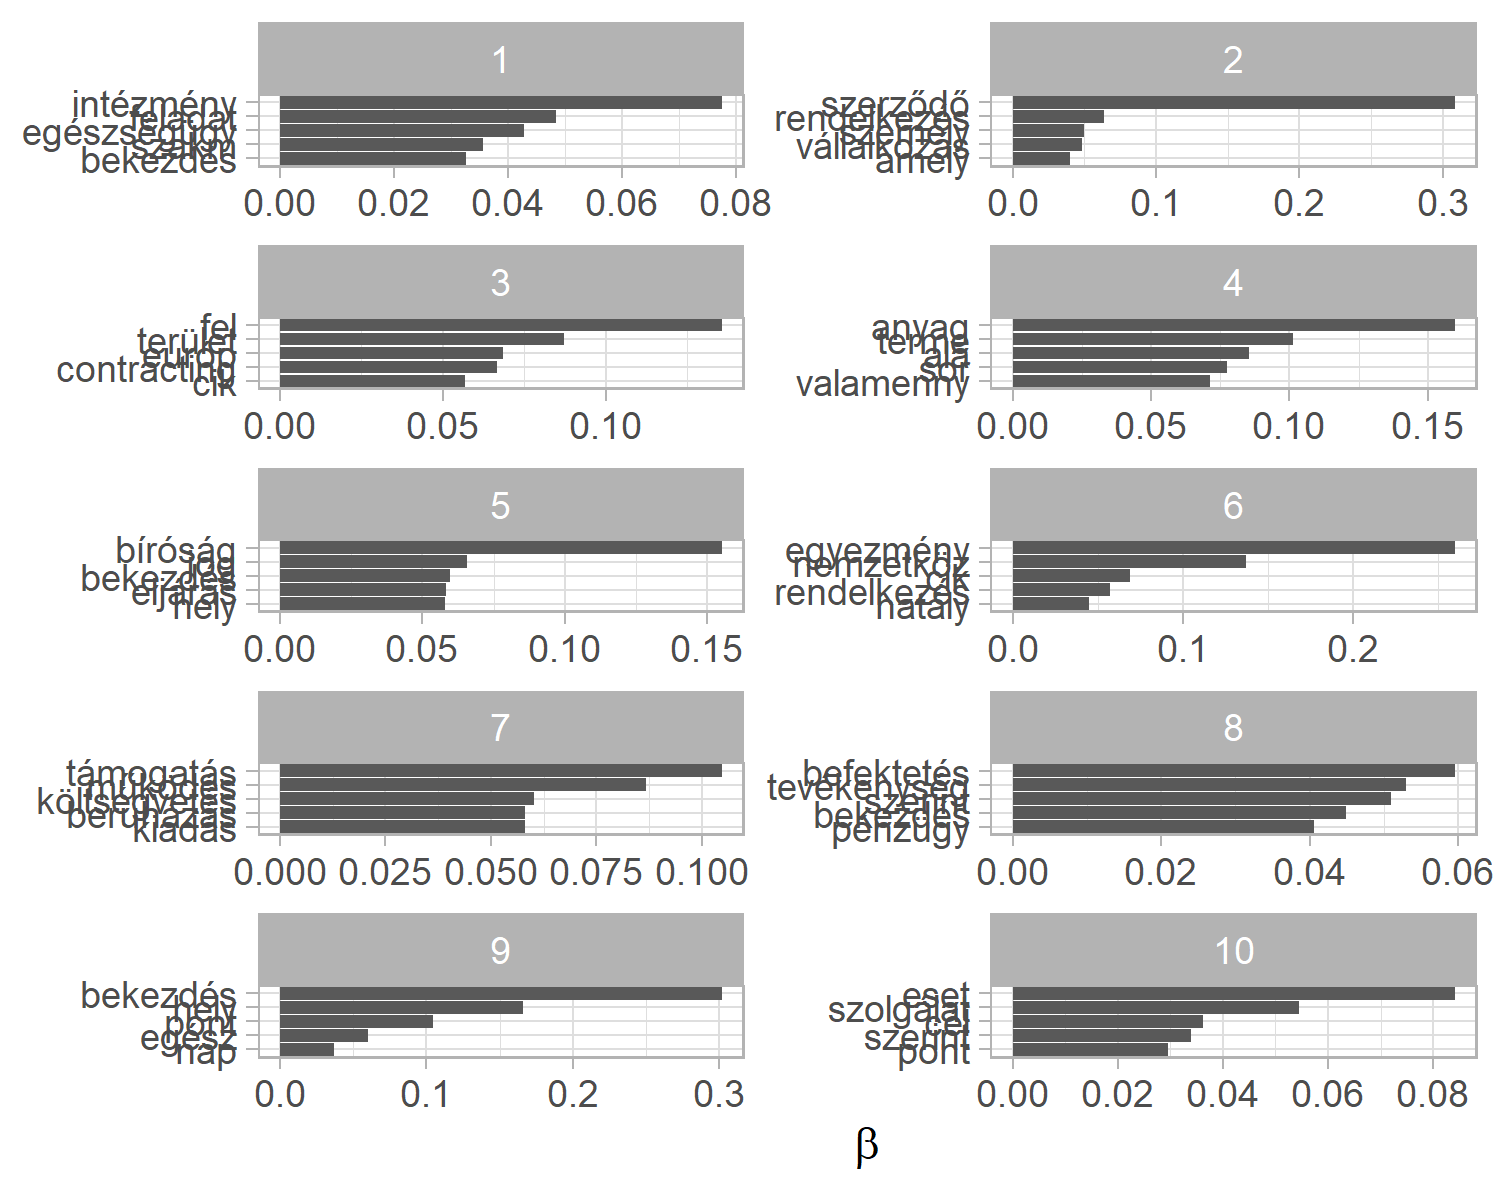
\includegraphics[width=0.9\linewidth]{_main_files/figure-latex/unnamed-chunk-120-1} \end{center}

Ahogy az előzőekben, itt is megváltoztathatjuk az ábra színét.

\begin{Shaded}
\begin{Highlighting}[]
\FunctionTok{ggplot}\NormalTok{(}
  \AttributeTok{data =}\NormalTok{ gapminder,}
  \AttributeTok{mapping =} \FunctionTok{aes}\NormalTok{(}
    \AttributeTok{x =}\NormalTok{ gdpPercap,}
    \AttributeTok{y =}\NormalTok{ lifeExp}
\NormalTok{  )}
\NormalTok{) }\SpecialCharTok{+}
  \FunctionTok{geom\_point}\NormalTok{(}\AttributeTok{colour =} \StringTok{"blue"}\NormalTok{)}
\end{Highlighting}
\end{Shaded}

\begin{center}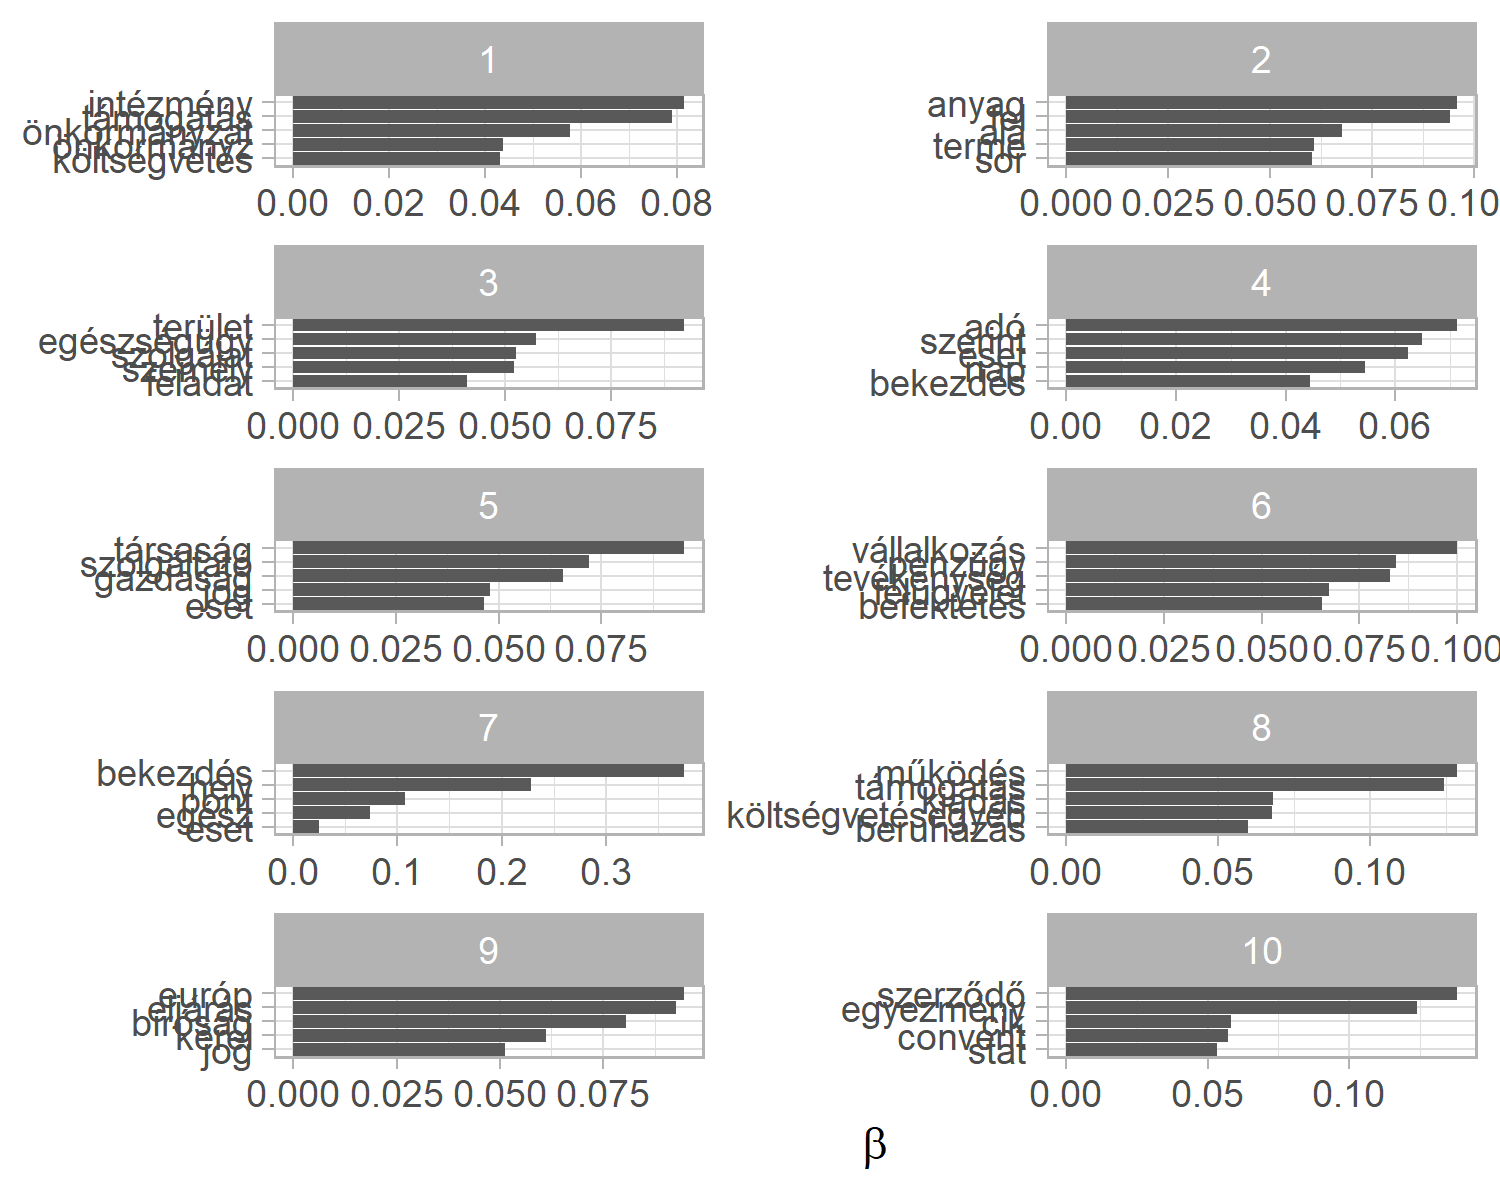
\includegraphics[width=0.9\linewidth]{_main_files/figure-latex/unnamed-chunk-121-1} \end{center}

Az fenti script kibővítésével az egyes kontinensek adatait különböző
színnel ábrázolhatjuk, az x és y tengelyt elnevezhetjük, a histogramnak
címet és alcímet adhatunk, illetve az adataink forrását is
feltüntethetjük az alábbi módon:

\begin{Shaded}
\begin{Highlighting}[]
\FunctionTok{ggplot}\NormalTok{(}
  \AttributeTok{data =}\NormalTok{ gapminder,}
  \AttributeTok{mapping =} \FunctionTok{aes}\NormalTok{(}
    \AttributeTok{x =}\NormalTok{ gdpPercap,}
    \AttributeTok{y =}\NormalTok{ lifeExp,}
    \AttributeTok{color =}\NormalTok{ continent}
\NormalTok{  )}
\NormalTok{) }\SpecialCharTok{+}
  \FunctionTok{geom\_point}\NormalTok{() }\SpecialCharTok{+}
  \FunctionTok{labs}\NormalTok{(}
    \AttributeTok{x =} \StringTok{"GDP per capita (log $)"}\NormalTok{,}
    \AttributeTok{y =} \StringTok{"Life expectancy"}\NormalTok{,}
    \AttributeTok{title =} \StringTok{"Connection between GDP and Life expectancy"}\NormalTok{,}
    \AttributeTok{subtitle =} \StringTok{"Points are country{-}years"}\NormalTok{,}
    \AttributeTok{caption =} \StringTok{"Source: Gapminder dataset"}
\NormalTok{  )}
\end{Highlighting}
\end{Shaded}

\begin{center}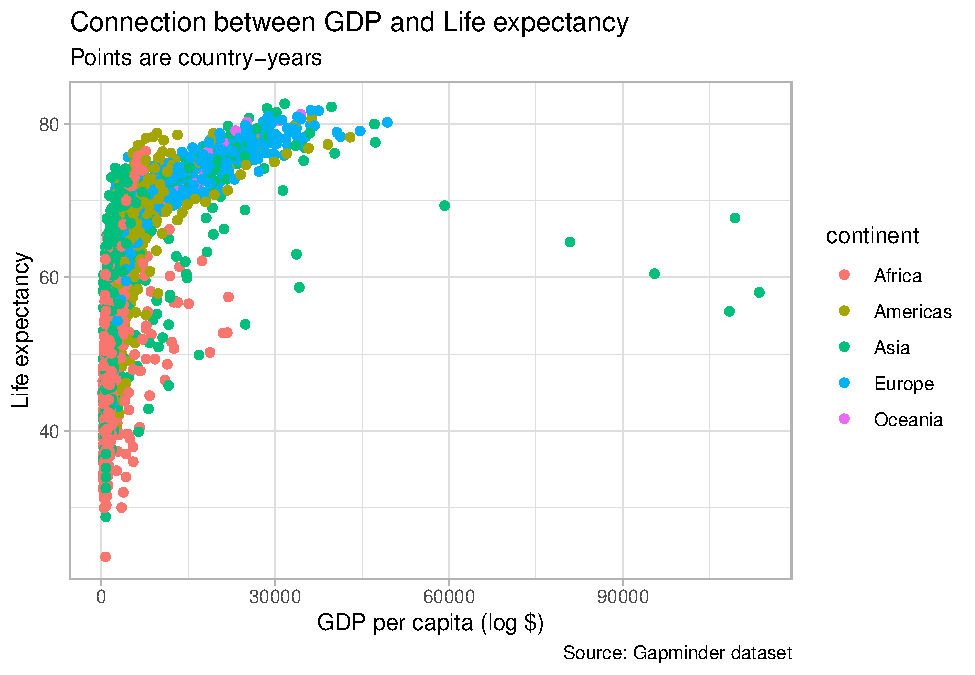
\includegraphics[width=0.9\linewidth]{_main_files/figure-latex/unnamed-chunk-122-1} \end{center}

Az ábrán található feliratok méretének, betűtípusának és betűszínének
megválasztásra is lehetőségünk van.

\begin{Shaded}
\begin{Highlighting}[]
\FunctionTok{ggplot}\NormalTok{(}
  \AttributeTok{data =}\NormalTok{ gapminder,}
  \AttributeTok{mapping =} \FunctionTok{aes}\NormalTok{(}
    \AttributeTok{x =}\NormalTok{ gdpPercap,}
    \AttributeTok{y =}\NormalTok{ lifeExp,}
    \AttributeTok{color =}\NormalTok{ continent}
\NormalTok{  )}
\NormalTok{) }\SpecialCharTok{+}
  \FunctionTok{geom\_point}\NormalTok{() }\SpecialCharTok{+}
  \FunctionTok{labs}\NormalTok{(}
    \AttributeTok{x =} \StringTok{"GDP per capita (log $)"}\NormalTok{,}
    \AttributeTok{y =} \StringTok{"Life expectancy"}\NormalTok{,}
    \AttributeTok{title =} \StringTok{"Connection between GDP and Life expectancy"}\NormalTok{,}
    \AttributeTok{subtitle =} \StringTok{"Points are country{-}years"}\NormalTok{,}
    \AttributeTok{caption =} \StringTok{"Source: Gapminder dataset"}
\NormalTok{  ) }\SpecialCharTok{+}
  \FunctionTok{theme}\NormalTok{(}\AttributeTok{plot.title =} \FunctionTok{element\_text}\NormalTok{(}
    \AttributeTok{size =} \DecValTok{12}\NormalTok{,}
    \AttributeTok{colour =} \StringTok{"red"}
\NormalTok{  ))}
\end{Highlighting}
\end{Shaded}

\begin{center}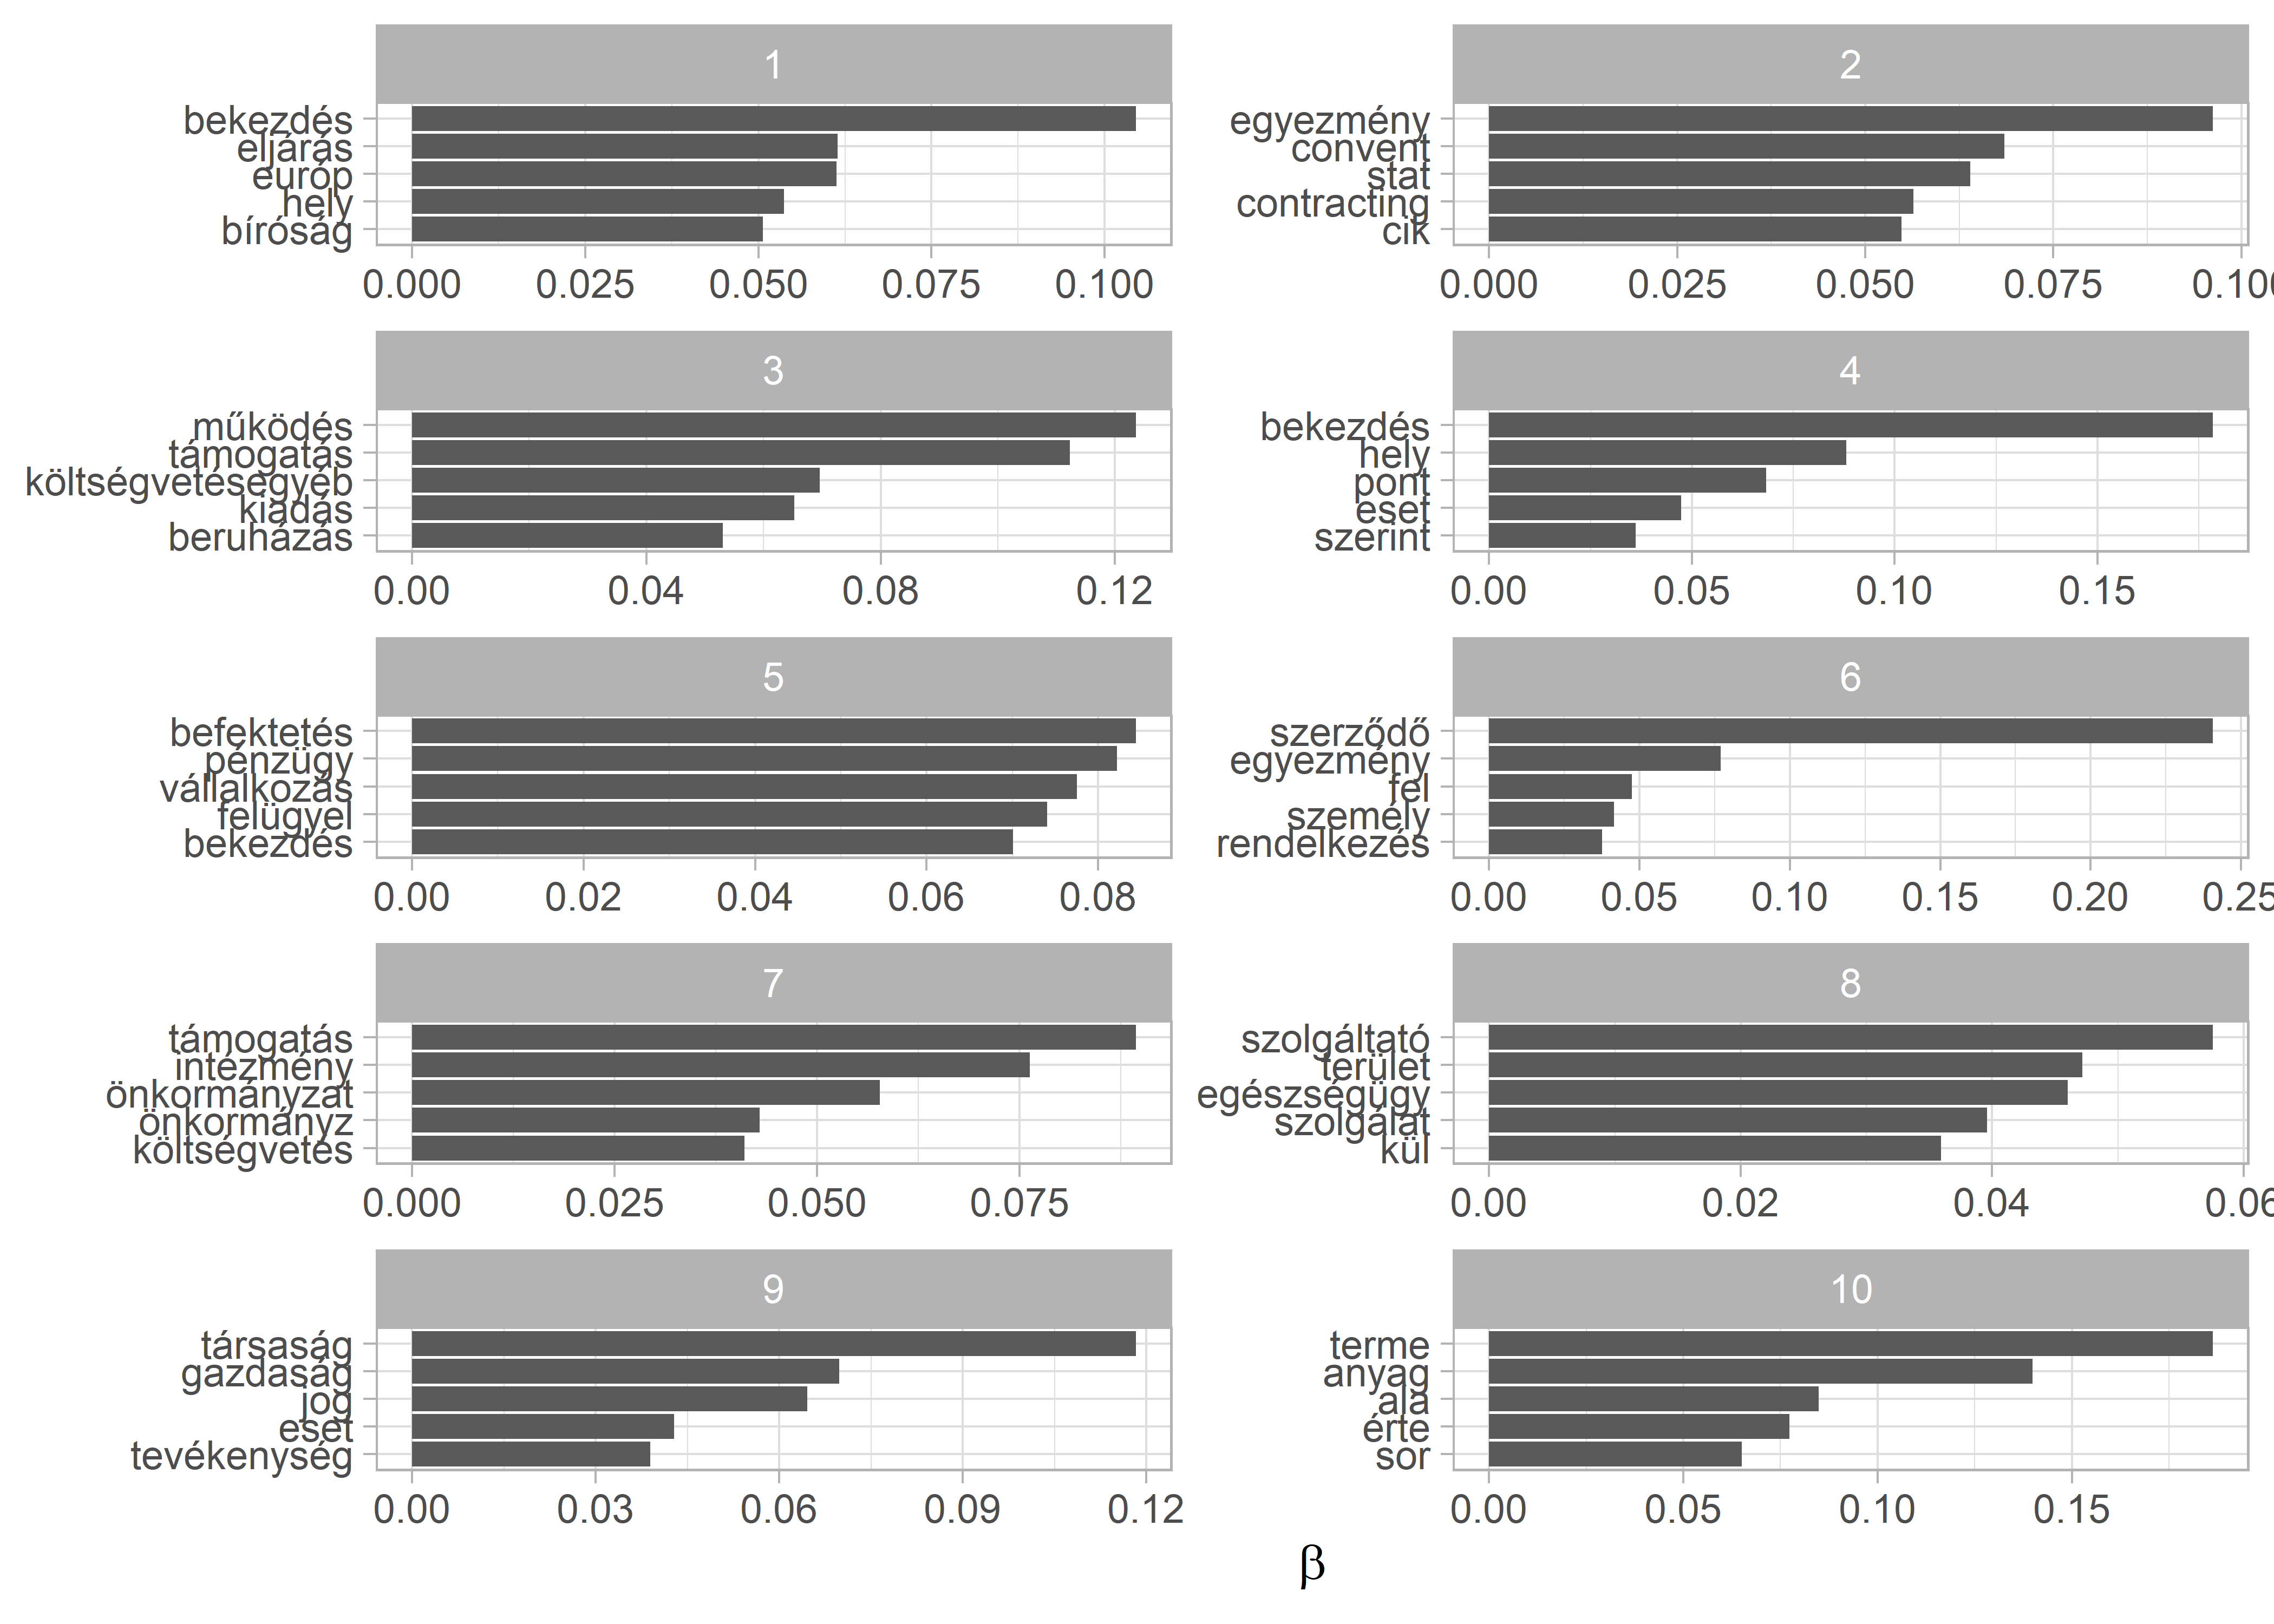
\includegraphics[width=0.9\linewidth]{_main_files/figure-latex/unnamed-chunk-123-1} \end{center}

Készíthetünk oszlopdiagramot is, amit a \texttt{ggplot2} diamonds
adatkészletén személtetünk

\begin{Shaded}
\begin{Highlighting}[]
\FunctionTok{ggplot}\NormalTok{(}\AttributeTok{data =}\NormalTok{ diamonds) }\SpecialCharTok{+}
  \FunctionTok{geom\_bar}\NormalTok{(}\AttributeTok{mapping =} \FunctionTok{aes}\NormalTok{(}\AttributeTok{x =}\NormalTok{ cut))}
\end{Highlighting}
\end{Shaded}

\begin{center}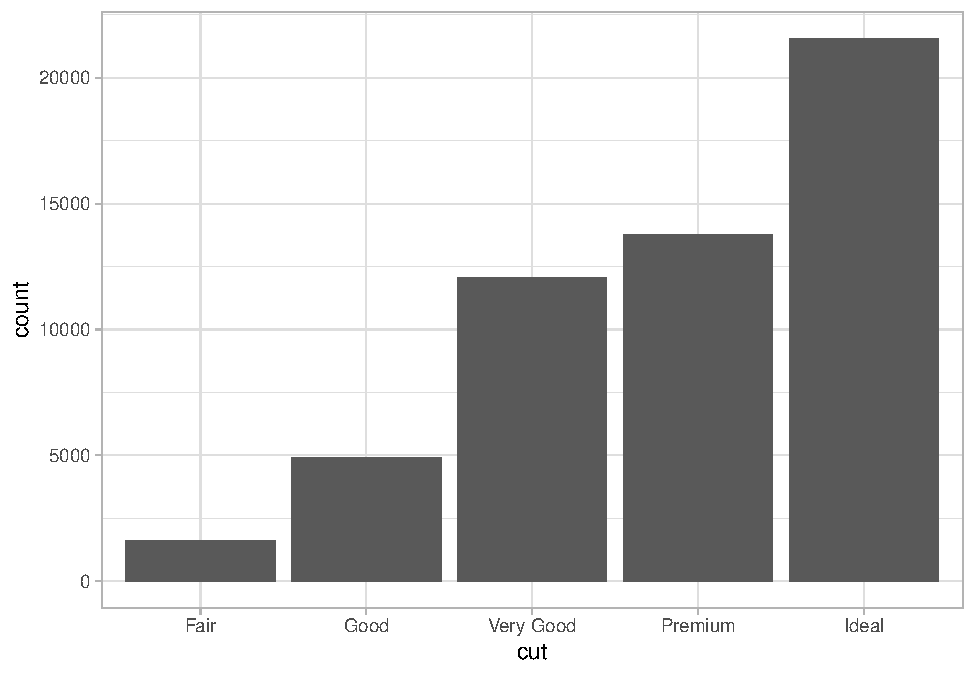
\includegraphics[width=0.9\linewidth]{_main_files/figure-latex/unnamed-chunk-124-1} \end{center}

Itt is lehetőségünk van arra, hogy a diagram színét megváltoztassuk.

\begin{Shaded}
\begin{Highlighting}[]
\FunctionTok{ggplot}\NormalTok{(}\AttributeTok{data =}\NormalTok{ diamonds) }\SpecialCharTok{+}
  \FunctionTok{geom\_bar}\NormalTok{(}\AttributeTok{mapping =} \FunctionTok{aes}\NormalTok{(}\AttributeTok{x =}\NormalTok{ cut), }\AttributeTok{fill =} \StringTok{"darkgreen"}\NormalTok{)}
\end{Highlighting}
\end{Shaded}

\begin{center}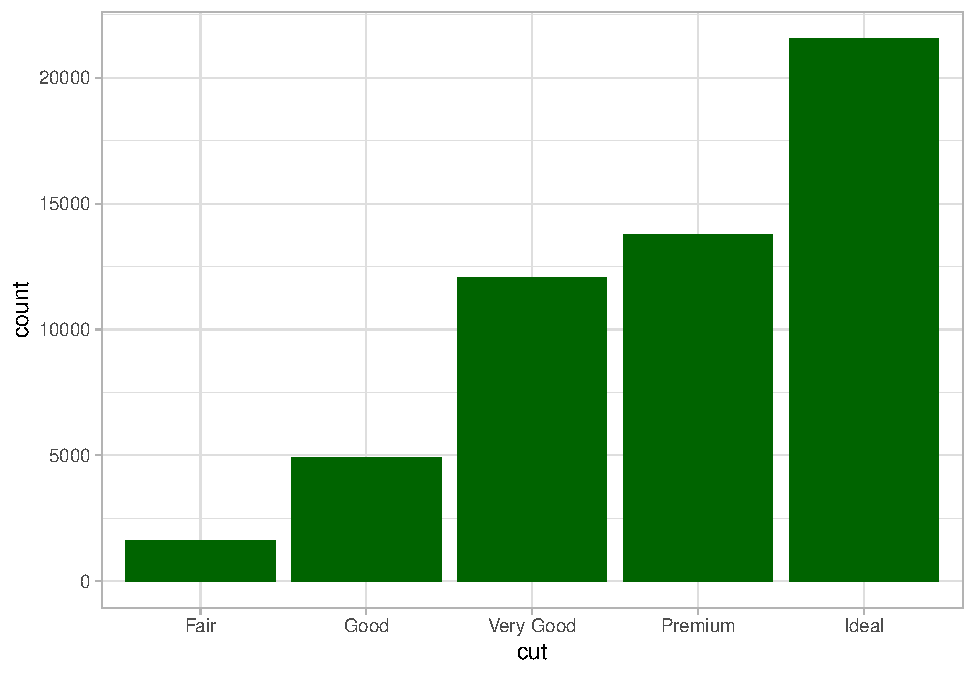
\includegraphics[width=0.9\linewidth]{_main_files/figure-latex/unnamed-chunk-125-1} \end{center}

De arra is lehetőségünk van, hogy az egyes oszlopok eltérő színűek
legyenek.

\begin{Shaded}
\begin{Highlighting}[]
\FunctionTok{ggplot}\NormalTok{(}\AttributeTok{data =}\NormalTok{ diamonds) }\SpecialCharTok{+}
  \FunctionTok{geom\_bar}\NormalTok{(}\AttributeTok{mapping =} \FunctionTok{aes}\NormalTok{(}\AttributeTok{x =}\NormalTok{ cut, }\AttributeTok{fill =}\NormalTok{ cut))}
\end{Highlighting}
\end{Shaded}

\begin{center}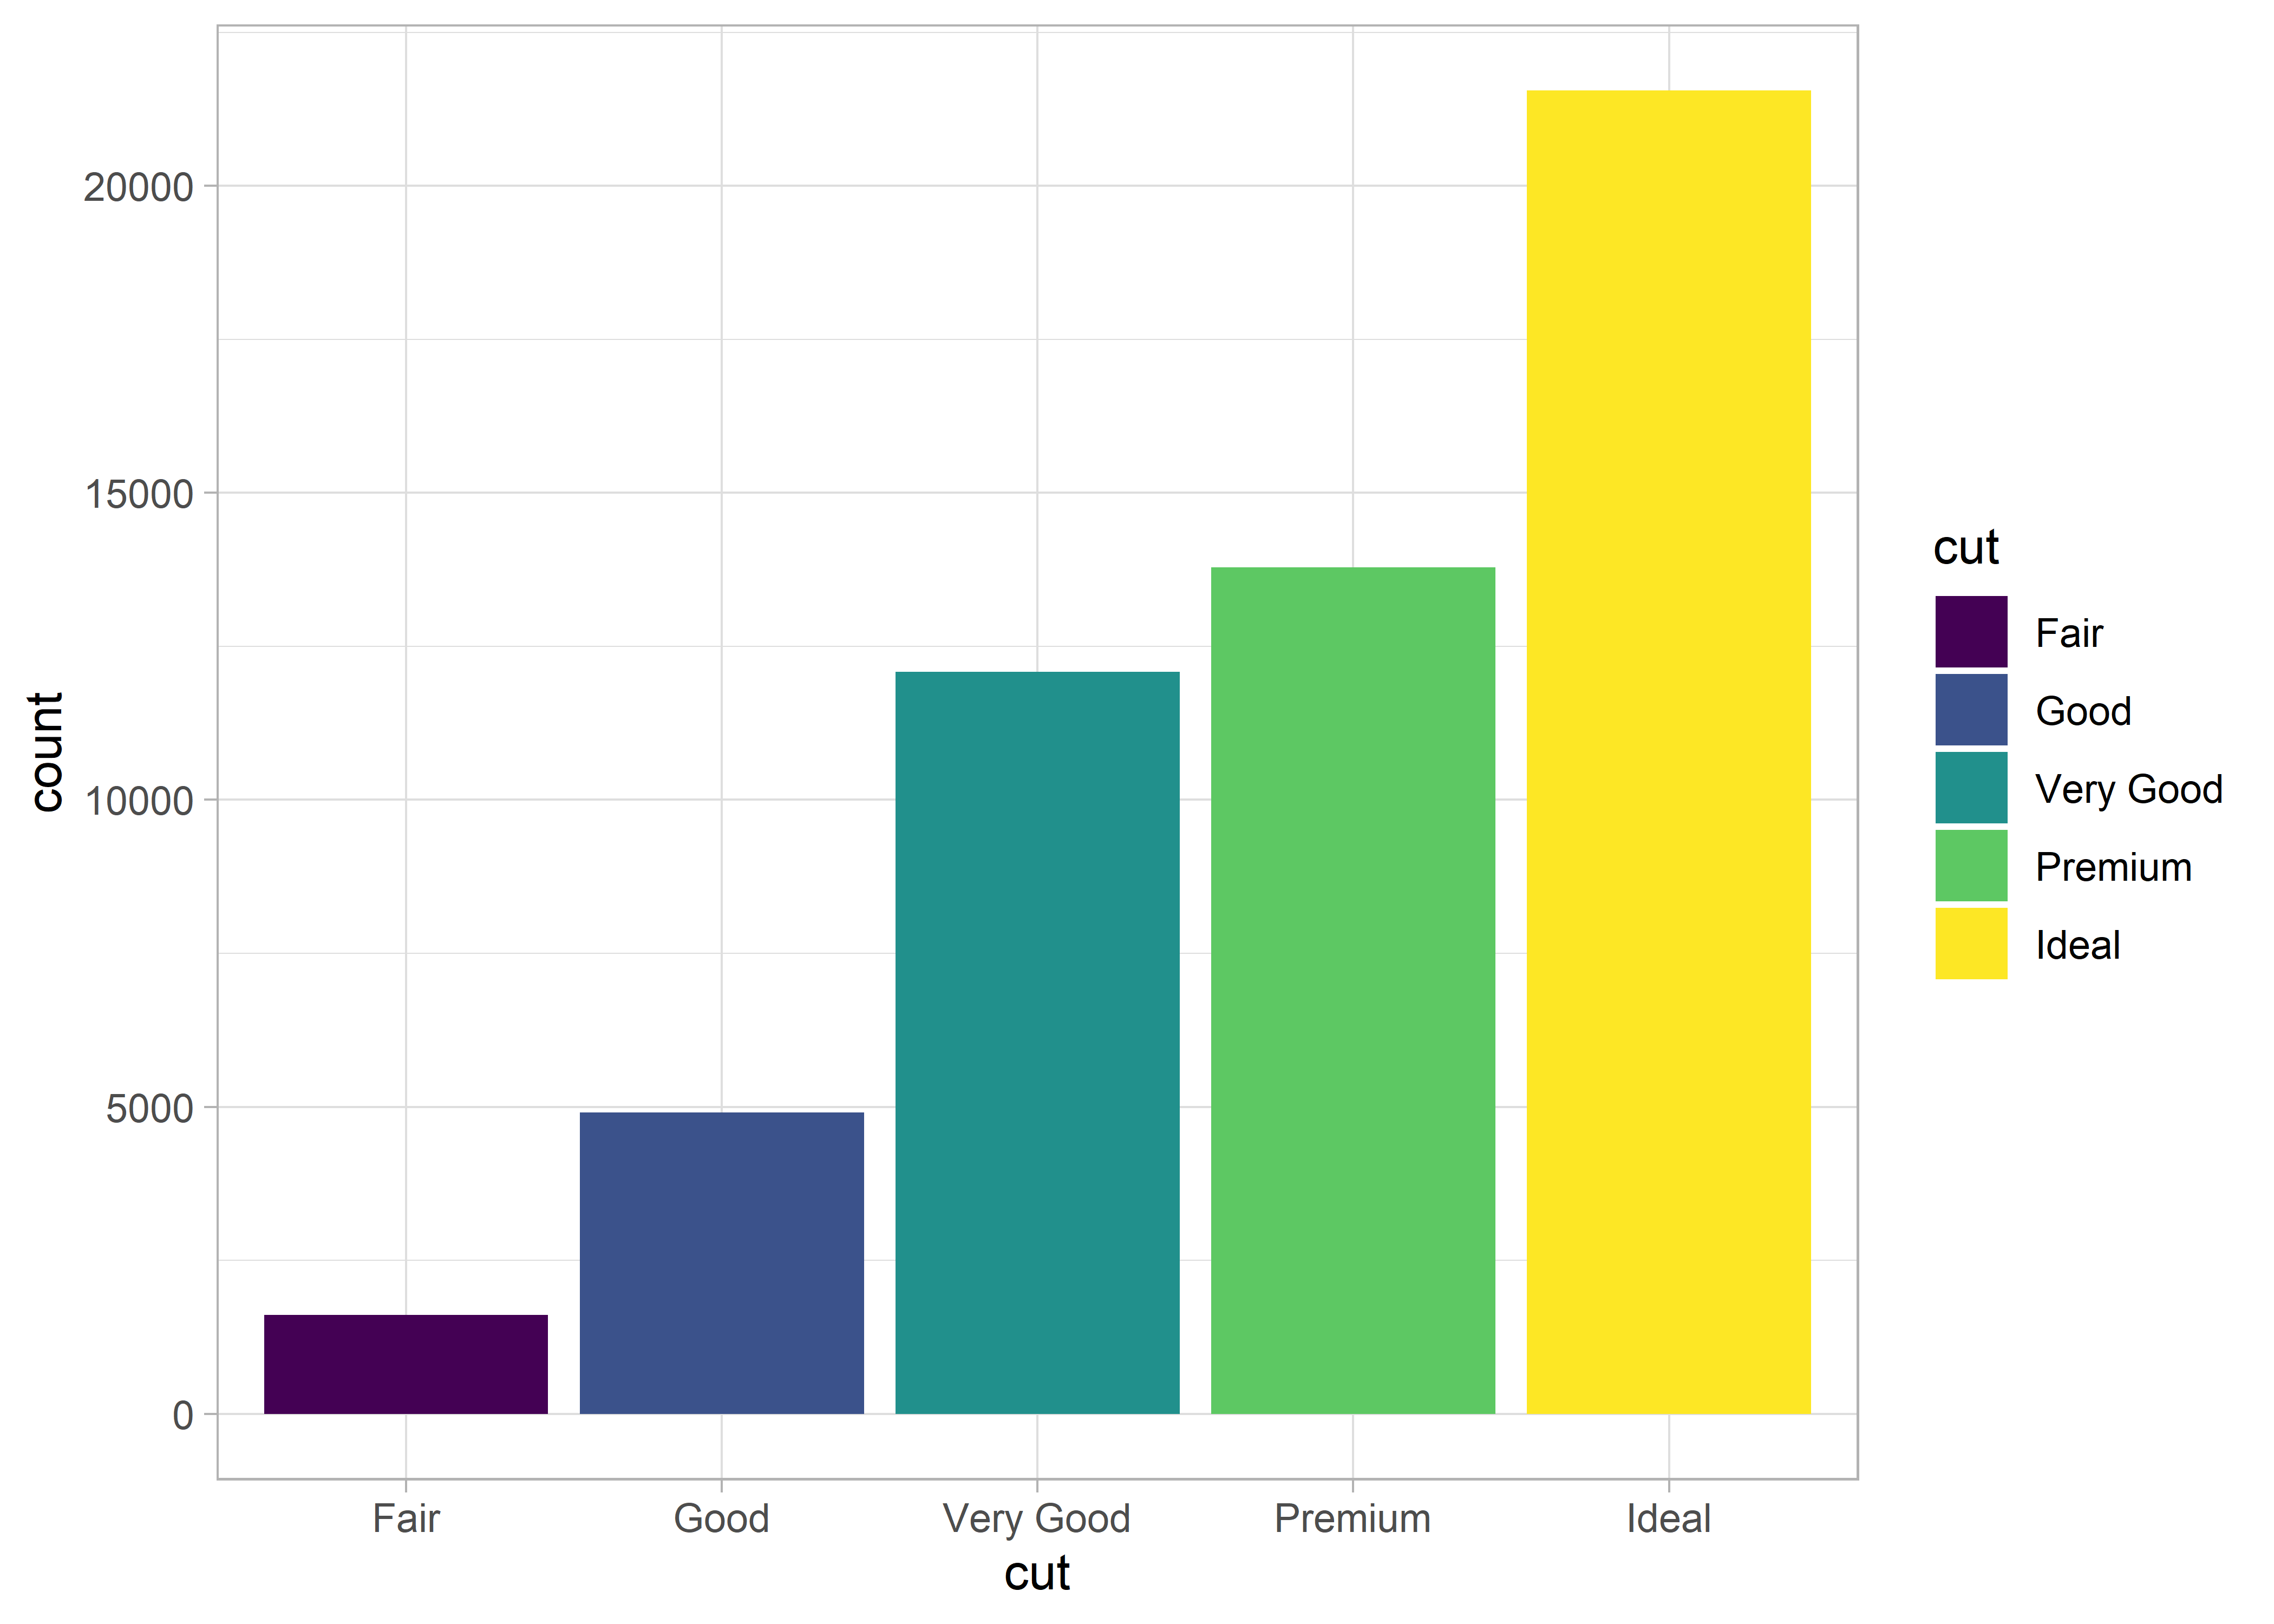
\includegraphics[width=0.9\linewidth]{_main_files/figure-latex/unnamed-chunk-126-1} \end{center}

Arra is van lehetőségünk, hogy egyszerre több változót is ábrázoljunk.

\begin{Shaded}
\begin{Highlighting}[]
\FunctionTok{ggplot}\NormalTok{(}\AttributeTok{data =}\NormalTok{ diamonds) }\SpecialCharTok{+}
  \FunctionTok{geom\_bar}\NormalTok{(}\AttributeTok{mapping =} \FunctionTok{aes}\NormalTok{(}\AttributeTok{x =}\NormalTok{ cut, }\AttributeTok{fill =}\NormalTok{ clarity))}
\end{Highlighting}
\end{Shaded}

\begin{center}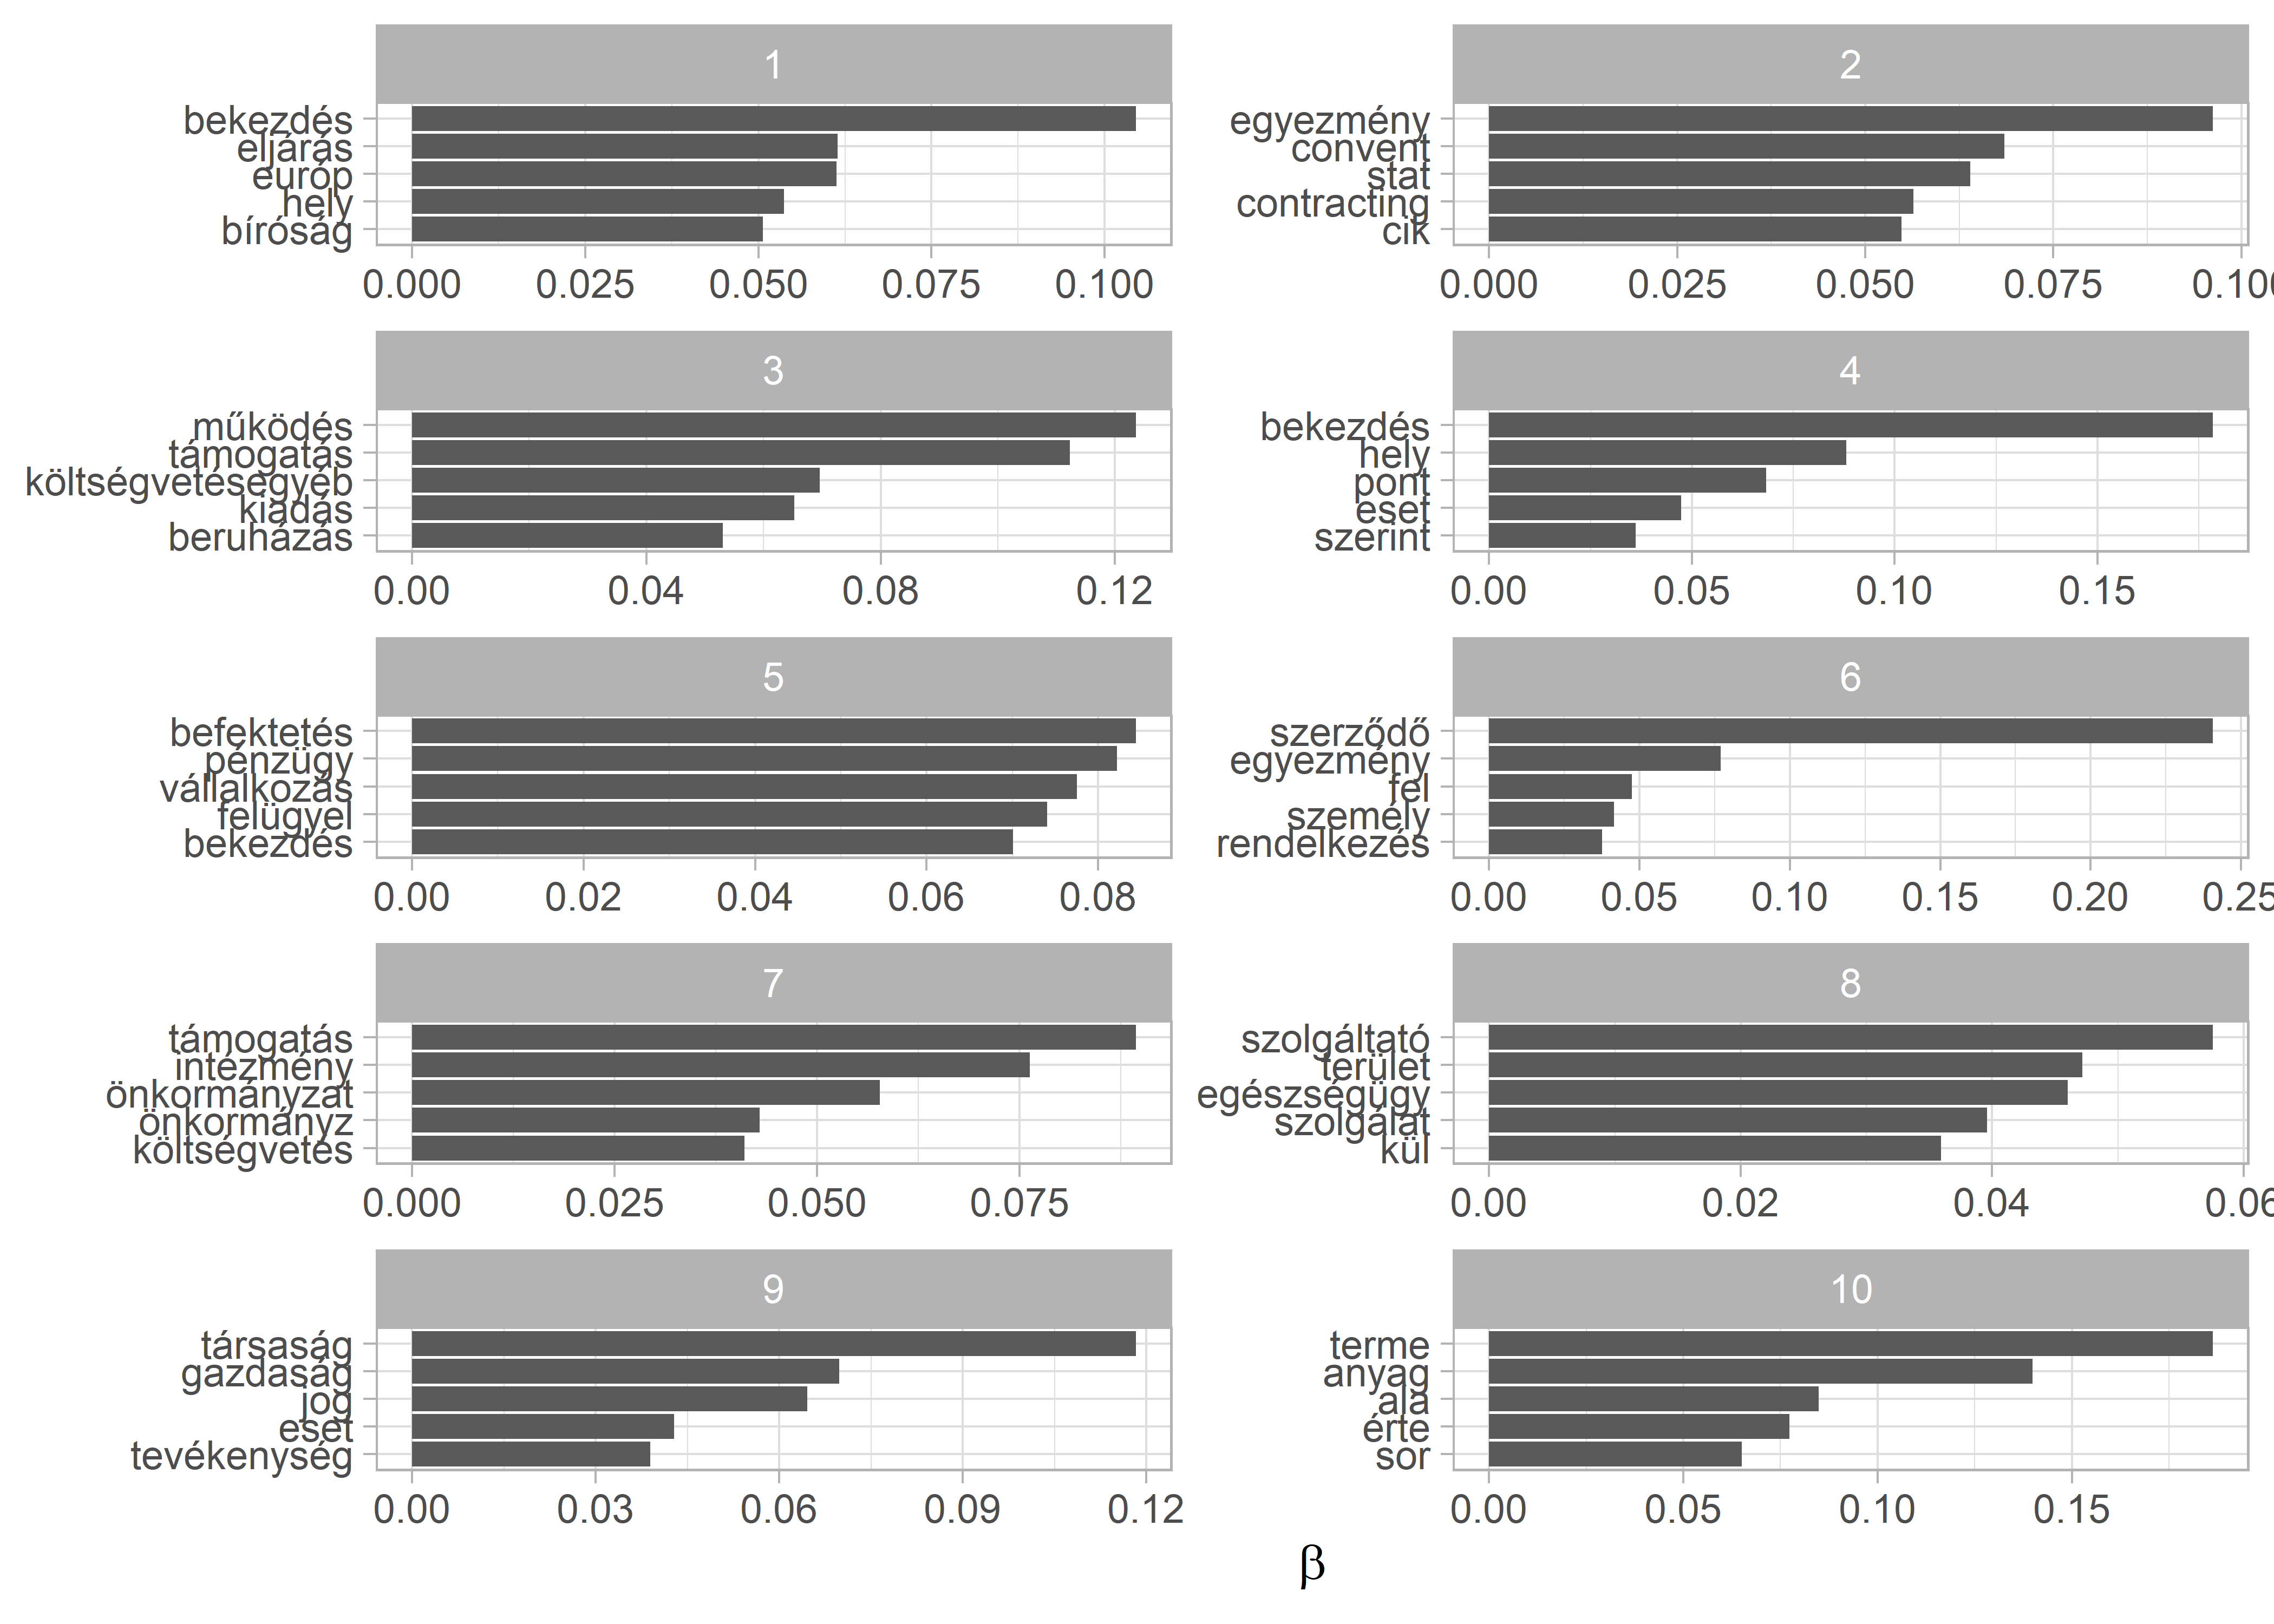
\includegraphics[width=0.9\linewidth]{_main_files/figure-latex/unnamed-chunk-127-1} \end{center}

Arra ggplot2 segítségével arra is lehetőségünk van, hogy csv-ből
beolvasott adatainkat vizualizáljuk.

\begin{Shaded}
\begin{Highlighting}[]
\NormalTok{plot\_cap\_1 }\OtherTok{\textless{}{-}} \FunctionTok{read.csv}\NormalTok{(}\StringTok{"data/plot\_cap\_1.csv"}\NormalTok{, }\AttributeTok{head =} \ConstantTok{TRUE}\NormalTok{, }\AttributeTok{sep =} \StringTok{";"}\NormalTok{)}
\FunctionTok{ggplot}\NormalTok{(plot\_cap\_1, }\FunctionTok{aes}\NormalTok{(Year, }\AttributeTok{fill =}\NormalTok{ Subtopic)) }\SpecialCharTok{+}
  \FunctionTok{scale\_x\_discrete}\NormalTok{(}\AttributeTok{limits =} \FunctionTok{c}\NormalTok{(}\DecValTok{1957}\NormalTok{, }\DecValTok{1958}\NormalTok{, }\DecValTok{1959}\NormalTok{, }\DecValTok{1960}\NormalTok{, }\DecValTok{1961}\NormalTok{, }\DecValTok{1962}\NormalTok{, }\DecValTok{1963}\NormalTok{)) }\SpecialCharTok{+}
  \FunctionTok{geom\_bar}\NormalTok{(}\AttributeTok{position =} \StringTok{"dodge"}\NormalTok{) }\SpecialCharTok{+}
  \FunctionTok{labs}\NormalTok{(}
    \AttributeTok{x =} \ConstantTok{NULL}\NormalTok{, }\AttributeTok{y =} \ConstantTok{NULL}\NormalTok{,}
    \AttributeTok{title =} \StringTok{"A Magyar Közlönyben kihirdetett agrárpolitikai jogszabályok"}\NormalTok{,}
    \AttributeTok{subtitle =} \StringTok{"N=445"}
\NormalTok{  ) }\SpecialCharTok{+}
  \FunctionTok{coord\_flip}\NormalTok{() }\SpecialCharTok{+} \CommentTok{\# az ábra tipusa}
  \FunctionTok{theme\_minimal}\NormalTok{() }\SpecialCharTok{+}
  \FunctionTok{theme}\NormalTok{(}\AttributeTok{plot.title =} \FunctionTok{element\_text}\NormalTok{(}\AttributeTok{size =} \DecValTok{12}\NormalTok{))}
\end{Highlighting}
\end{Shaded}

A csv-ből belolvasott adatainból kördiagramot is készíthetünk

\begin{Shaded}
\begin{Highlighting}[]
\NormalTok{pie }\OtherTok{\textless{}{-}} \FunctionTok{read.csv}\NormalTok{(}\StringTok{"data/pie.csv"}\NormalTok{, }\AttributeTok{head =} \ConstantTok{TRUE}\NormalTok{, }\AttributeTok{sep =} \StringTok{";"}\NormalTok{)}

\FunctionTok{ggplot}\NormalTok{(pie, }\FunctionTok{aes}\NormalTok{(}\AttributeTok{x =} \StringTok{""}\NormalTok{, }\AttributeTok{y =}\NormalTok{ value, }\AttributeTok{fill =}\NormalTok{ Type)) }\SpecialCharTok{+}
  \FunctionTok{geom\_bar}\NormalTok{(}\AttributeTok{stat =} \StringTok{"identity"}\NormalTok{, }\AttributeTok{width =} \DecValTok{1}\NormalTok{) }\SpecialCharTok{+}
  \FunctionTok{coord\_polar}\NormalTok{(}\StringTok{"y"}\NormalTok{, }\AttributeTok{start =} \DecValTok{0}\NormalTok{) }\SpecialCharTok{+}
  \FunctionTok{scale\_fill\_brewer}\NormalTok{(}\AttributeTok{palette =} \StringTok{"GnBu"}\NormalTok{) }\SpecialCharTok{+}
  \FunctionTok{labs}\NormalTok{(}
    \AttributeTok{title =} \StringTok{"A Magyar Közlönyben megjelent jogszabályok típusai"}\NormalTok{,}
    \AttributeTok{subtitle =} \StringTok{"N = 445"}
\NormalTok{  ) }\SpecialCharTok{+}
  \FunctionTok{theme\_void}\NormalTok{()}
\end{Highlighting}
\end{Shaded}

\hypertarget{refs}{}
\begin{CSLReferences}{1}{0}
\leavevmode\hypertarget{ref-arun2010finding}{}%
Arun, Rajkumar, Venkatasubramaniyan Suresh, CE Veni Madhavan, and MN
Narasimha Murthy. 2010. {``On Finding the Natural Number of Topics with
Latent Dirichlet Allocation: Some Observations.''} In, 391402.

\leavevmode\hypertarget{ref-cao2009density}{}%
Cao, Juan, Tian Xia, Jintao Li, Yongdong Zhang, and Sheng Tang. 2009.
{``A Density-Based Method for Adaptive LDA Model Selection.''}
\emph{Neurocomputing} 72 (7-9): 17751781.

\leavevmode\hypertarget{ref-deveaud2014accurate}{}%
Deveaud, Romain, Eric SanJuan, and Patrice Bellot. 2014. {``Accurate and
Effective Latent Concept Modeling for Ad Hoc Information Retrieval.''}
\emph{Document Numérique} 17 (1): 6184.

\leavevmode\hypertarget{ref-griffiths2004}{}%
Griffiths, T. L., and M. Steyvers. 2004. {``Finding Scientific
Topics.''} \emph{Proceedings of the National Academy of Sciences} 101
(Supplement 1): 5228--35. \url{https://doi.org/10.1073/pnas.0307752101}.

\leavevmode\hypertarget{ref-grimmer2013text}{}%
Grimmer, Justin, and Brandon M Stewart. 2013. {``Text as Data: The
Promise and Pitfalls of Automatic Content Analysis Methods for Political
Texts.''} \emph{Political Analysis} 21 (3): 267297.

\leavevmode\hypertarget{ref-jacobi2016}{}%
Jacobi, Carina, Wouter Van Atteveldt, and Kasper Welbers. 2016.
{``Quantitative Analysis of Large Amounts of Journalistic Texts Using
Topic Modelling.''} \emph{Digital Journalism} 4 (1): 89--106.

\leavevmode\hypertarget{ref-laver2000estimating}{}%
Laver, Michael, and John Garry. 2000. {``Estimating Policy Positions
from Political Texts.''} \emph{American Journal of Political Science},
619634.

\leavevmode\hypertarget{ref-loughran2011}{}%
Loughran, Tim, and Bill McDonald. 2011. {``When Is a Liability Not a
Liability? Textual Analysis, Dictionaries, and 10-Ks.''} \emph{The
Journal of Finance} 66 (1): 35--65.

\leavevmode\hypertarget{ref-muxe1tuxe92021}{}%
Máté, Ákos, Miklós Sebők, and Tamás Barczikay. 2021. {``The Effect of
Central Bank Communication on Sovereign Bond Yields: The Case of
Hungary.''} Edited by Hiranya K. Nath. \emph{PLOS ONE} 16 (2): e0245515.
\url{https://doi.org/10.1371/journal.pone.0245515}.

\leavevmode\hypertarget{ref-roberts2014structural}{}%
Roberts, Margaret E, Brandon M Stewart, Dustin Tingley, Christopher
Lucas, Jetson Leder-Luis, Shana Kushner Gadarian, Bethany Albertson, and
David G Rand. 2014. {``Structural Topic Models for Open-Ended Survey
Responses.''} \emph{American Journal of Political Science} 58 (4):
10641082.

\leavevmode\hypertarget{ref-silge2017text}{}%
Silge, Julia, and David Robinson. 2017. \emph{Text Mining with r: A Tidy
Approach}. {"} O'Reilly Media, Inc.{"}.

\leavevmode\hypertarget{ref-wickham2016r}{}%
Wickham, Hadley, and Garrett Grolemund. 2016. \emph{R for Data Science:
Import, Tidy, Transform, Visualize, and Model Data}. {"} O'Reilly Media,
Inc.{"}.

\leavevmode\hypertarget{ref-young2012affective}{}%
Young, Lori, and Stuart Soroka. 2012. {``Affective News: The Automated
Coding of Sentiment in Political Texts.''} \emph{Political
Communication} 29 (2): 205231.

\end{CSLReferences}

\backmatter
\end{document}
